%&preformat-disser
\RequirePackage[l2tabu,orthodox]{nag} % Раскомментировав, можно в логе получать рекомендации относительно правильного использования пакетов и предупреждения об устаревших и нерекомендуемых пакетах
% Формат А4, 14pt (ГОСТ Р 7.0.11-2011, 5.3.6)
\documentclass[a4paper,14pt,oneside,openany]{memoir}

%% Режим черновика
\makeatletter
\@ifundefined{c@draft}{
  \newcounter{draft}
  \setcounter{draft}{0}  % 0 --- чистовик (максимальное соблюдение ГОСТ)
                         % 1 --- черновик (отклонения от ГОСТ, но быстрая сборка итоговых PDF)
}{}
\makeatother

%% Использование в pdflatex шрифтов не по-умолчанию
\makeatletter
\@ifundefined{c@usealtfont}{
  \newcounter{usealtfont}
  \setcounter{usealtfont}{1}    % 0 --- шрифты на базе Computer Modern
                                % 1 --- использовать пакет pscyr, при его наличии
                                % 2 --- использовать пакет XCharter, при наличии подходящей версии
}{}
\makeatother

%% Библиография

%% Внимание! При использовании bibtex8 необходимо удалить все
%% цитирования из  ../common/characteristic.tex
\makeatletter
\@ifundefined{c@bibliosel}{
  \newcounter{bibliosel}
  \setcounter{bibliosel}{1}           % 0 --- встроенная реализация с загрузкой файла через движок bibtex8; 1 --- реализация пакетом biblatex через движок biber
}{}
\makeatother

%%% Предкомпиляция tikz рисунков для ускорения работы %%%
\makeatletter
\@ifundefined{c@imgprecompile}{
  \newcounter{imgprecompile}
  \setcounter{imgprecompile}{0}   % 0 --- без предкомпиляции;
                                  % 1 --- пользоваться предварительно скомпилированными pdf вместо генерации заново из tikz
}{}
\makeatother
               % общие настройки шаблона
%%% Проверка используемого TeX-движка %%%
\RequirePackage{ifxetex, ifluatex}
\newif\ifxetexorluatex   % определяем новый условный оператор (http://tex.stackexchange.com/a/47579)
\ifxetex
    \xetexorluatextrue
\else
    \ifluatex
        \xetexorluatextrue
    \else
        \xetexorluatexfalse
    \fi
\fi

\newif\ifsynopsis           % Условие, проверяющее, что документ --- автореферат

\RequirePackage{etoolbox}[2015/08/02]               % Для продвинутой проверки разных условий

%%% Поля и разметка страницы %%%
\usepackage{pdflscape}                              % Для включения альбомных страниц
\usepackage{geometry}                               % Для последующего задания полей

%%% Математические пакеты %%%
\usepackage{amsthm,amsmath,amscd}       % Математические дополнения от AMS
\ifxetexorluatex
    \usepackage{amsfonts,amssymb}       % Математические дополнения от AMS
\else
    \ifnumequal{\value{usealtfont}}{2}{}{
        \usepackage{amsfonts,amssymb}       % Математические дополнения от AMS
    }
\fi
\usepackage{mathtools}                  % Добавляет окружение multlined

%%%% Установки для размера шрифта 14 pt %%%%
%% Формирование переменных и констант для сравнения (один раз для всех подключаемых файлов)%%
%% должно располагаться до вызова пакета fontspec или polyglossia, потому что они сбивают его работу
\newlength{\curtextsize}
\newlength{\bigtextsize}
\setlength{\bigtextsize}{13.9pt}

\makeatletter
%\show\f@size                                       % неплохо для отслеживания, но вызывает стопорение процесса, если документ компилируется без команды  -interaction=nonstopmode 
\setlength{\curtextsize}{\f@size pt}
\makeatother

%%% Кодировки и шрифты %%%
\ifxetexorluatex
    \usepackage{polyglossia}[2014/05/21]            % Поддержка многоязычности (fontspec подгружается автоматически)
\else
   %%% Решение проблемы копирования текста в буфер кракозябрами
    \ifnumequal{\value{usealtfont}}{1}{% Используется pscyr, при наличии
        \IfFileExists{pscyr.sty}{% вероятно, без pscyr нет необходимости в этом коде
            \input glyphtounicode.tex
            \input glyphtounicode-cmr.tex %from pdfx package
            \pdfgentounicode=1
        }{}
    }{}
    \usepackage{cmap}                               % Улучшенный поиск русских слов в полученном pdf-файле
    \defaulthyphenchar=127                          % Если стоит до fontenc, то переносы не впишутся в выделяемый текст при копировании его в буфер обмена 
    \usepackage[T1,T2A]{fontenc}                    % Поддержка русских букв
    \ifnumequal{\value{usealtfont}}{1}{% Используется pscyr, при наличии
        \IfFileExists{pscyr.sty}{\usepackage{pscyr}}{}  % Подключение pscyr
    }{}
    \usepackage[utf8]{inputenc}[2014/04/30]         % Кодировка utf8
    \usepackage[english, russian]{babel}[2014/03/24]% Языки: русский, английский
    \ifnumequal{\value{usealtfont}}{2}{
        % http://dxdy.ru/post1238763.html#p1238763
        \usepackage[scaled=0.925]{XCharter}[2017/06/25] % Подключение русифицированных шрифтов XCharter
        \usepackage[bitstream-charter]{mathdesign} % Согласование математических шрифтов
    }{}
\fi

%%% Оформление абзацев %%%
\usepackage{indentfirst}                            % Красная строка

%%% Цвета %%%
\usepackage[dvipsnames, table, hyperref, cmyk]{xcolor} % Совместимо с tikz. Конвертация всех цветов в cmyk заложена как удовлетворение возможного требования типографий. Возможно конвертирование и в rgb.

%%% Таблицы %%%
\usepackage{longtable,ltcaption}                    % Длинные таблицы
\usepackage{multirow,makecell}                      % Улучшенное форматирование таблиц

%%% Общее форматирование
\usepackage{soulutf8}                               % Поддержка переносоустойчивых подчёркиваний и зачёркиваний
\usepackage{icomma}                                 % Запятая в десятичных дробях
\usepackage[hyphenation, lastparline]{impnattypo}   % Оптимизация расстановки переносов и длины последней строки абзаца

%%% Гиперссылки %%%
\usepackage{hyperref}[2012/11/06]

%%% Изображения %%%
\usepackage{graphicx}[2014/04/25]                   % Подключаем пакет работы с графикой

%%% Списки %%%
\usepackage{enumitem}

%%% Счётчики %%%
\usepackage[figure,table]{totalcount}               % Счётчик рисунков и таблиц
\usepackage{totcount}                               % Пакет создания счётчиков на основе последнего номера подсчитываемого элемента (может требовать дважды компилировать документ)
\usepackage{totpages}                               % Счётчик страниц, совместимый с hyperref (ссылается на номер последней страницы). Желательно ставить последним пакетом в преамбуле

%%% Продвинутое управление групповыми ссылками (пока только формулами) %%%
\ifxetexorluatex
    \usepackage{cleveref}                           % cleveref корректно считывает язык из настроек polyglossia
\else
    \usepackage[russian]{cleveref}                  % cleveref имеет сложности со считыванием языка из babel. Такое решение русификации вывода выбрано вместо определения в documentclass из опасности что-то лишнее передать во все остальные пакеты, включая библиографию.
\fi
\creflabelformat{equation}{#2#1#3}                  % Формат по умолчанию ставил круглые скобки вокруг каждого номера ссылки, теперь просто номера ссылок без какого-либо дополнительного оформления
\crefrangelabelformat{equation}{#3#1#4\cyrdash#5#2#6}   % Интервалы в русском языке принято делать через тире, если иное не оговорено


\ifnumequal{\value{draft}}{1}{% Черновик
    \usepackage[firstpage]{draftwatermark}
    \SetWatermarkText{DRAFT}
    \SetWatermarkFontSize{14pt}
    \SetWatermarkScale{15}
    \SetWatermarkAngle{45}
}{}

%%% Цитата, не приводимая в автореферате:
% возможно, актуальна только для biblatex
%\newcommand{\citeinsynopsis}[1]{\ifsynopsis\else ~\cite{#1} \fi}
  % Пакеты общие для диссертации и автореферата
\synopsisfalse                           % Этот документ --- не автореферат
%%% Прикладные пакеты %%% 
%\usepackage{calc}               % Пакет для расчётов параметров, например длины

%%% Для добавления Стр. над номерами страниц в оглавлении
%%% http://tex.stackexchange.com/a/306950
\usepackage{afterpage}

\usepackage{tikz}                   % Продвинутый пакет векторной графики
\usetikzlibrary{chains}             % Для примера tikz рисунка
\usetikzlibrary{shapes.geometric}   % Для примера tikz рисунка
\usetikzlibrary{shapes.symbols}     % Для примера tikz рисунка
\usetikzlibrary{arrows}             % Для примера tikz рисунка
\ifnumequal{\value{imgprecompile}}{1}{% Только если у нас включена предкомпиляция
    \usetikzlibrary{external}   % подключение возможности предкомпиляции
    \tikzexternalize[prefix=Dissertation/images/] % activate! % здесь можно указать отдельную папку для скомпилированных файлов
}{}
         % Пакеты для диссертации
\usepackage{tabu, tabulary}  %таблицы с автоматически подбирающейся шириной столбцов
\usepackage{fr-longtable}    %ради \endlasthead

% Листинги с исходным кодом программ
\usepackage{fancyvrb}
\usepackage{listings}
\lccode`\~=0\relax %Без этого хака из-за особенностей пакета listings перестают работать конструкции с \MakeLowercase и т. п. в (xe|lua)latex

% Русская традиция начертания греческих букв
\usepackage{upgreek} % прямые греческие ради русской традиции

% Микротипографика
%\ifnumequal{\value{draft}}{0}{% Только если у нас режим чистовика
%    \usepackage[final]{microtype}[2016/05/14] % улучшает представление букв и слов в строках, может помочь при наличии отдельно висящих слов
%}{}

% Отметка о версии черновика на каждой странице
% Чтобы работало надо в своей локальной копии по инструкции
% https://www.ctan.org/pkg/gitinfo2 создать небходимые файлы в папке
% ./git/hooks
% If you’re familiar with tweaking git, you can probably work it out for
% yourself. If not, I suggest you follow these steps:
% 1. First, you need a git repository and working tree. For this example,
% let’s suppose that the root of the working tree is in ~/compsci
% 2. Copy the file post-xxx-sample.txt (which is in the same folder of
% your TEX distribution as this pdf) into the git hooks directory in your
% working copy. In our example case, you should end up with a file called
% ~/compsci/.git/hooks/post-checkout
% 3. If you’re using a unix-like system, don’t forget to make the file executable.
% Just how you do this is outside the scope of this manual, but one
% possible way is with commands such as this:
% chmod g+x post-checkout.
% 4. Test your setup with “git checkout master” (or another suitable branch
% name). This should generate copies of gitHeadInfo.gin in the directories
% you intended.
% 5. Now make two more copies of this file in the same directory (hooks),
% calling them post-commit and post-merge, and you’re done. As before,
% users of unix-like systems should ensure these files are marked as
% executable.
\ifnumequal{\value{draft}}{1}{% Черновик
   \IfFileExists{.git/gitHeadInfo.gin}{                                        
      \usepackage[mark,pcount]{gitinfo2}
      \renewcommand{\gitMark}{rev.\gitAbbrevHash\quad\gitCommitterEmail\quad\gitAuthorIsoDate}
      \renewcommand{\gitMarkFormat}{\rmfamily\color{Gray}\small\bfseries}
   }{}
}{}        % Пакеты для специфических пользовательских задач

%%%%%%%%%%%%%%%%%%%%%%%%%%%%%%%%%%%%%%%%%%%%%%%%%%%%%%
%%%% Файл упрощённых настроек шаблона диссертации %%%%
%%%%%%%%%%%%%%%%%%%%%%%%%%%%%%%%%%%%%%%%%%%%%%%%%%%%%%

%%% Инициализирование переменных, не трогать!  %%%
\newcounter{intvl}
\newcounter{otstup}
\newcounter{contnumeq}
\newcounter{contnumfig}
\newcounter{contnumtab}
\newcounter{pgnum}
\newcounter{chapstyle}
\newcounter{headingdelim}
\newcounter{headingalign}
\newcounter{headingsize}
\newcounter{tabcap}
\newcounter{tablaba}
\newcounter{tabtita}
\newcounter{usefootcite}
%%%%%%%%%%%%%%%%%%%%%%%%%%%%%%%%%%%%%%%%%%%%%%%%%%

%%% Область упрощённого управления оформлением %%%

%% Интервал между заголовками и между заголовком и текстом
% Заголовки отделяют от текста сверху и снизу тремя интервалами (ГОСТ Р 7.0.11-2011, 5.3.5)
\setcounter{intvl}{3}               % Коэффициент кратности к размеру шрифта

%% Отступы у заголовков в тексте
\setcounter{otstup}{0}              % 0 --- без отступа; 1 --- абзацный отступ

%% Нумерация формул, таблиц и рисунков
\setcounter{contnumeq}{0}           % Нумерация формул: 0 --- пораздельно (во введении подряд, без номера раздела); 1 --- сквозная нумерация по всей диссертации
\setcounter{contnumfig}{0}          % Нумерация рисунков: 0 --- пораздельно (во введении подряд, без номера раздела); 1 --- сквозная нумерация по всей диссертации
\setcounter{contnumtab}{1}          % Нумерация таблиц: 0 --- пораздельно (во введении подряд, без номера раздела); 1 --- сквозная нумерация по всей диссертации

%% Оглавление
\setcounter{pgnum}{1}               % 0 --- номера страниц никак не обозначены; 1 --- Стр. над номерами страниц (дважды компилировать после изменения)
\settocdepth{subsection}            % до какого уровня подразделов выносить в оглавление
\setsecnumdepth{subsection}         % до какого уровня нумеровать подразделы


%% Текст и форматирование заголовков
\setcounter{chapstyle}{1}           % 0 --- разделы только под номером; 1 --- разделы с названием "Глава" перед номером
\setcounter{headingdelim}{1}        % 0 --- номер отделен пропуском в 1em или \quad; 1 --- номера разделов и приложений отделены точкой с пробелом, подразделы пропуском без точки; 2 --- номера разделов, подразделов и приложений отделены точкой с пробелом.

%% Выравнивание заголовков в тексте
\setcounter{headingalign}{0}        % 0 --- по центру; 1 --- по левому краю

%% Размеры заголовков в тексте
\setcounter{headingsize}{0}         % 0 --- по ГОСТ, все всегда 14 пт; 1 --- пропорционально изменяющийся размер в зависимости от базового шрифта

%% Подпись таблиц
\setcounter{tabcap}{0}              % 0 --- по ГОСТ, номер таблицы и название разделены тире, выровнены по левому краю, при необходимости на нескольких строках; 1 --- подпись таблицы не по ГОСТ, на двух и более строках, дальнейшие настройки: 
%Выравнивание первой строки, с подписью и номером
\setcounter{tablaba}{2}             % 0 --- по левому краю; 1 --- по центру; 2 --- по правому краю
%Выравнивание строк с самим названием таблицы
\setcounter{tabtita}{1}             % 0 --- по левому краю; 1 --- по центру; 2 --- по правому краю
%Разделитель записи «Таблица #» и названия таблицы
\newcommand{\tablabelsep}{ }

%% Подпись рисунков
%Разделитель записи «Рисунок #» и названия рисунка
\newcommand{\figlabelsep}{~\cyrdash\ } % (ГОСТ 2.105, 4.3.1) % "--- здесь не работает

%%% Цвета гиперссылок %%%
% Latex color definitions: http://latexcolor.com/
\definecolor{linkcolor}{rgb}{0.9,0,0}
\definecolor{citecolor}{rgb}{0,0.6,0}
\definecolor{urlcolor}{rgb}{0,0,1}
%\definecolor{linkcolor}{rgb}{0,0,0} %black
%\definecolor{citecolor}{rgb}{0,0,0} %black
%\definecolor{urlcolor}{rgb}{0,0,0} %black
               % Упрощённые настройки шаблона

%%% Переопределение именований, чтобы можно было и в преамбуле использовать %%%
\renewcommand{\chaptername}{Глава}
\renewcommand{\appendixname}{Приложение} % (ГОСТ Р 7.0.11-2011, 5.7)
       % Переопределение именований, чтобы можно было и в преамбуле использовать
% Новые переменные, которые могут использоваться во всём проекте
% ГОСТ 7.0.11-2011
% 9.2 Оформление текста автореферата диссертации
% 9.2.1 Общая характеристика работы включает в себя следующие основные структурные
% элементы:
% актуальность темы исследования;
\newcommand{\actualityTXT}{Актуальность темы.}
% степень ее разработанности;
\newcommand{\progressTXT}{Степень разработанности темы.}
% цели и задачи;
\newcommand{\aimTXT}{Целью}
\newcommand{\tasksTXT}{задачи}
% научную новизну;
\newcommand{\noveltyTXT}{Научная новизна:}
% теоретическую и практическую значимость работы;
%\newcommand{\influenceTXT}{Теоретическая и практическая значимость}
% или чаще используют просто
\newcommand{\influenceTXT}{Практическая значимость}
% методологию и методы исследования;
\newcommand{\methodsTXT}{Mетодология и методы исследования.}
% положения, выносимые на защиту;
\newcommand{\defpositionsTXT}{Основные положения, выносимые на~защиту:}
% степень достоверности и апробацию результатов.
\newcommand{\reliabilityTXT}{Достоверность}
\newcommand{\probationTXT}{Апробация работы.}

\newcommand{\contributionTXT}{Личный вклад.}
\newcommand{\publicationsTXT}{Публикации.}


\newcommand{\authorbibtitle}{Публикации автора по теме диссертации}
\newcommand{\vakbibtitle}{В изданиях из списка ВАК РФ}
\newcommand{\notvakbibtitle}{В прочих изданиях}
\newcommand{\confbibtitle}{В сборниках трудов конференций}
\newcommand{\fullbibtitle}{Список литературы} % (ГОСТ Р 7.0.11-2011, 4)

\newcommand{\Cp}[1]{\mathbf{C}^{\mathbf{#1 #1}}} % кросс-спектр
\newcommand{\Tf}[1]{\hat{\mathbf{#1}}} %
\newcommand*\conj[1]{#1^*}
\newcommand*\Expect[1]{\mathbf{E}\Big\{#1\Big\}}
% \newcommand*\abs[1]{\lvert#1\rvert}

\DeclarePairedDelimiter\abs{\lvert}{\rvert}%
\makeatletter
\let\oldabs\abs
\def\abs{\@ifstar{\oldabs}{\oldabs*}}
\makeatother

% \newcommand*\def[1]{\stackrel{def}{#1}}
\newcommand\defeq{\mathrel{\overset{\makebox[0pt]{\mbox{\normalfont\tiny\sffamily def}}}{=}}}
% \newcommand*\Laplace{\mathop{}\!\mathbin\bigtriangleup}
\newcommand*\Laplace{\Delta}

\newcommand{\norm}[1]{\left\lVert#1\right\rVert}
\DeclarePairedDelimiter\set\{\}
\DeclareMathOperator{\tr}{tr}
\DeclareMathOperator{\coh}{coh}
\DeclareMathOperator{\sign}{sign}
\DeclareMathOperator*{\argmin}{arg\,min}
\DeclareMathOperator{\prox}{prox}
\DeclareMathOperator{\diag}{diag}
\DeclareMathOperator*{\argmax}{arg\,max}
\DeclareMathOperator*{\trace}{Tr}

\def\D{\mathrm{d}}  % differential

% matrices and vectors typesetting
\newcommand{\mG}{\mathbf{G}} % matrix G
\newcommand{\vs}{\mathbf{s}} % vector s
\newcommand{\vx}{\mathbf{x}} % vector x
\newcommand{\vomega}{\boldsymbol{\omega}} % vector omega

\renewcommand{\vec}[1]{\mathbf{#1}}
\newcommand{\matr}[1]{\mathbf{#1}}
  % Новые переменные, которые могут использоваться во всём проекте

%%% Основные сведения %%%
\newcommand{\thesisAuthorLastName}{\todo{Алтухов}}
\newcommand{\thesisAuthorOtherNames}{\todo{Дмитрий Игоревич}}
\newcommand{\thesisAuthorInitials}{\todo{Д.\,И.}}
\newcommand{\thesisAuthor}             % Диссертация, ФИО автора
{%
    \texorpdfstring{% \texorpdfstring takes two arguments and uses the first for (La)TeX and the second for pdf
        \thesisAuthorLastName~\thesisAuthorOtherNames% так будет отображаться на титульном листе или в тексте, где будет использоваться переменная
    }{%
        \thesisAuthorLastName, \thesisAuthorOtherNames% эта запись для свойств pdf-файла. В таком виде, если pdf будет обработан программами для сбора библиографических сведений, будет правильно представлена фамилия.
    }
}
\newcommand{\thesisAuthorShort}        % Диссертация, ФИО автора инициалами
{\thesisAuthorInitials~\thesisAuthorLastName}
%\newcommand{\thesisUdk}                % Диссертация, УДК
%{\todo{xxx.xxx}}
\newcommand{\thesisTitle}              % Диссертация, название
{\todo{ Использование методов глобальной разреженной оптимизации для обнаружения функционально-синхронных участков коры головного мозга на основании неинвазивных МЭГ данных.}}
\newcommand{\thesisSpecialtyNumber}    % Диссертация, специальность, номер
{\todo{05.13.01}}
\newcommand{\thesisSpecialtyTitle}     % Диссертация, специальность, название
{\todo{Системный анализ, управление и обработка информации}}
\newcommand{\thesisDegree}             % Диссертация, ученая степень
{\todo{кандидата физико-математических наук}}
\newcommand{\thesisDegreeShort}        % Диссертация, ученая степень, краткая запись
{\todo{канд. физ.-мат. наук}}
\newcommand{\thesisCity}               % Диссертация, город написания диссертации
{\todo{Москва}}
\newcommand{\thesisYear}               % Диссертация, год написания диссертации
{\todo{2017}}
\newcommand{\thesisOrganization}       % Диссертация, организация
{\todo{Национальный Исследоваетельский Университет Высшая Школа Экономики}}
\newcommand{\thesisOrganizationShort}  % Диссертация, краткое название организации для доклада
{\todo{НИУ ВШЭ}}

\newcommand{\thesisInOrganization}     % Диссертация, организация в предложном падеже: Работа выполнена в ...
{\todo{Национальном Исследовательском Унивеситете Высшая Школа Экономики}}

\newcommand{\supervisorFio}            % Научный руководитель, ФИО
{\todo{Осадчий Алексей Евгениевич}}
\newcommand{\supervisorRegalia}        % Научный руководитель, регалии
{\todo{PhD, проофессор}}
\newcommand{\supervisorFioShort}       % Научный руководитель, ФИО
{\todo{А.\,Е.~Осадчий}}
\newcommand{\supervisorRegaliaShort}   % Научный руководитель, регалии
{\todo{PhD.,~проф.}}


\newcommand{\opponentOneFio}           % Оппонент 1, ФИО
{\todo{Фамилия Имя Отчество}}
\newcommand{\opponentOneRegalia}       % Оппонент 1, регалии
{\todo{доктор физико-математических наук, профессор}}
\newcommand{\opponentOneJobPlace}      % Оппонент 1, место работы
{\todo{Не очень длинное название для места работы}}
\newcommand{\opponentOneJobPost}       % Оппонент 1, должность
{\todo{старший научный сотрудник}}

\newcommand{\opponentTwoFio}           % Оппонент 2, ФИО
{\todo{Фамилия Имя Отчество}}
\newcommand{\opponentTwoRegalia}       % Оппонент 2, регалии
{\todo{кандидат физико-математических наук}}
\newcommand{\opponentTwoJobPlace}      % Оппонент 2, место работы
{\todo{Основное место работы c длинным длинным длинным длинным названием}}
\newcommand{\opponentTwoJobPost}       % Оппонент 2, должность
{\todo{старший научный сотрудник}}

\newcommand{\leadingOrganizationTitle} % Ведущая организация, дополнительные строки
{\todo{Федеральное государственное бюджетное образовательное учреждение высшего профессионального образования с~длинным длинным длинным длинным названием}}

\newcommand{\defenseDate}              % Защита, дата
{\todo{DD mmmmmmmm YYYY~г.~в~XX часов}}
\newcommand{\defenseCouncilNumber}     % Защита, номер диссертационного совета
{\todo{Д\,123.456.78}}
\newcommand{\defenseCouncilTitle}      % Защита, учреждение диссертационного совета
{\todo{Название учреждения}}
\newcommand{\defenseCouncilAddress}    % Защита, адрес учреждение диссертационного совета
{\todo{Адрес}}
\newcommand{\defenseCouncilPhone}      % Телефон для справок
{\todo{+7~(0000)~00-00-00}}

\newcommand{\defenseSecretaryFio}      % Секретарь диссертационного совета, ФИО
{\todo{Фамилия Имя Отчество}}
\newcommand{\defenseSecretaryRegalia}  % Секретарь диссертационного совета, регалии
{\todo{д-р~физ.-мат. наук}}            % Для сокращений есть ГОСТы, например: ГОСТ Р 7.0.12-2011 + http://base.garant.ru/179724/#block_30000

\newcommand{\synopsisLibrary}          % Автореферат, название библиотеки
{\todo{Название библиотеки}}
\newcommand{\synopsisDate}             % Автореферат, дата рассылки
{\todo{DD mmmmmmmm YYYY года}}

% To avoid conflict with beamer class use \providecommand
\providecommand{\keywords}%            % Ключевые слова для метаданных PDF диссертации и автореферата
{}
      % Основные сведения
%%% Шаблон %%%
\DeclareRobustCommand{\todo}{\textcolor{red}}       % решаем проблему превращения названия цвета в результате \MakeUppercase, http://tex.stackexchange.com/a/187930/79756 , \DeclareRobustCommand protects \todo from expanding inside \MakeUppercase
\AtBeginDocument{%
    \setlength{\parindent}{2.5em}                   % Абзацный отступ. Должен быть одинаковым по всему тексту и равен пяти знакам (ГОСТ Р 7.0.11-2011, 5.3.7).
}

%%% Кодировки и шрифты %%%
\ifxetexorluatex
    \setmainlanguage[babelshorthands=true]{russian}  % Язык по-умолчанию русский с поддержкой приятных команд пакета babel
    \setotherlanguage{english}                       % Дополнительный язык = английский (в американской вариации по-умолчанию)
    \setmonofont{Courier New}                        % моноширинный шрифт
    \newfontfamily\cyrillicfonttt{Courier New}       % моноширинный шрифт для кириллицы
    \defaultfontfeatures{Ligatures=TeX}              % стандартные лигатуры TeX, замены нескольких дефисов на тире и т. п. Настройки моноширинного шрифта должны идти до этой строки, чтобы при врезках кода программ в коде не применялись лигатуры и замены дефисов
    \setmainfont{Times New Roman}                    % Шрифт с засечками
    \newfontfamily\cyrillicfont{Times New Roman}     % Шрифт с засечками для кириллицы
    \setsansfont{Arial}                              % Шрифт без засечек
    \newfontfamily\cyrillicfontsf{Arial}             % Шрифт без засечек для кириллицы
\else
    \ifnumequal{\value{usealtfont}}{1}{% Используется pscyr, при наличии
        \IfFileExists{pscyr.sty}{\renewcommand{\rmdefault}{ftm}}{}
    }{}
\fi

%%% Подписи %%%
\setlength{\abovecaptionskip}{0pt}   % Отбивка над подписью
\setlength{\belowcaptionskip}{0pt}   % Отбивка под подписью
\captionwidth{\linewidth}
\normalcaptionwidth

%%% Таблицы %%%
\ifnumequal{\value{tabcap}}{0}{%
    \newcommand{\tabcapalign}{\raggedright}  % по левому краю страницы или аналога parbox
    \renewcommand{\tablabelsep}{~\cyrdash\ } % тире как разделитель идентификатора с номером от наименования
    \newcommand{\tabtitalign}{}
}{%
    \ifnumequal{\value{tablaba}}{0}{%
        \newcommand{\tabcapalign}{\raggedright}  % по левому краю страницы или аналога parbox
    }{}

    \ifnumequal{\value{tablaba}}{1}{%
        \newcommand{\tabcapalign}{\centering}    % по центру страницы или аналога parbox
    }{}

    \ifnumequal{\value{tablaba}}{2}{%
        \newcommand{\tabcapalign}{\raggedleft}   % по правому краю страницы или аналога parbox
    }{}

    \ifnumequal{\value{tabtita}}{0}{%
        \newcommand{\tabtitalign}{\par\raggedright}  % по левому краю страницы или аналога parbox
    }{}

    \ifnumequal{\value{tabtita}}{1}{%
        \newcommand{\tabtitalign}{\par\centering}    % по центру страницы или аналога parbox
    }{}

    \ifnumequal{\value{tabtita}}{2}{%
        \newcommand{\tabtitalign}{\par\raggedleft}   % по правому краю страницы или аналога parbox
    }{}
}

\precaption{\tabcapalign} % всегда идет перед подписью или \legend
\captionnamefont{\normalfont\normalsize} % Шрифт надписи «Таблица #»; также определяет шрифт у \legend
\captiondelim{\tablabelsep} % разделитель идентификатора с номером от наименования
\captionstyle[\tabtitalign]{\tabtitalign}
\captiontitlefont{\normalfont\normalsize} % Шрифт с текстом подписи

%%% Рисунки %%%
\setfloatadjustment{figure}{%
    \setlength{\abovecaptionskip}{0pt}   % Отбивка над подписью
    \setlength{\belowcaptionskip}{0pt}   % Отбивка под подписью
    \precaption{} % всегда идет перед подписью или \legend
    \captionnamefont{\normalfont\normalsize} % Шрифт надписи «Рисунок #»; также определяет шрифт у \legend
    \captiondelim{\figlabelsep} % разделитель идентификатора с номером от наименования
    \captionstyle[\centering]{\centering} % Центрирование подписей, заданных командой \caption и \legend
    \captiontitlefont{\normalfont\normalsize} % Шрифт с текстом подписи
    \postcaption{} % всегда идет после подписи или \legend, и с новой строки
}

%%% Подписи подрисунков %%%
\newsubfloat{figure} % Включает возможность использовать подрисунки у окружений figure
\renewcommand{\thesubfigure}{\asbuk{subfigure}}           % Буквенные номера подрисунков
\subcaptionsize{\normalsize} % Шрифт подписи названий подрисунков (не отличается от основного)
\subcaptionlabelfont{\normalfont}
\subcaptionfont{\!\!) \normalfont} % Вот так тут добавили скобку после буквы.
\subcaptionstyle{\centering}
%\subcaptionsize{\fontsize{12pt}{13pt}\selectfont} % объявляем шрифт 12pt для использования в подписях, тут же надо интерлиньяж объявлять, если не наследуется

%%% Настройки гиперссылок %%%
\ifluatex
    \hypersetup{
        unicode,                % Unicode encoded PDF strings
    }
\fi

\hypersetup{
    linktocpage=true,           % ссылки с номера страницы в оглавлении, списке таблиц и списке рисунков
%    linktoc=all,                % both the section and page part are links
%    pdfpagelabels=false,        % set PDF page labels (true|false)
    plainpages=false,           % Forces page anchors to be named by the Arabic form  of the page number, rather than the formatted form
    colorlinks,                 % ссылки отображаются раскрашенным текстом, а не раскрашенным прямоугольником, вокруг текста
    linkcolor={linkcolor},      % цвет ссылок типа ref, eqref и подобных
    citecolor={citecolor},      % цвет ссылок-цитат
    urlcolor={urlcolor},        % цвет гиперссылок
%    hidelinks,                  % Hide links (removing color and border)
    pdftitle={\thesisTitle},    % Заголовок
    pdfauthor={\thesisAuthor},  % Автор
    pdfsubject={\thesisSpecialtyNumber\ \thesisSpecialtyTitle},      % Тема
%    pdfcreator={Создатель},     % Создатель, Приложение
%    pdfproducer={Производитель},% Производитель, Производитель PDF
    pdfkeywords={\keywords},    % Ключевые слова
    pdflang={ru},
}
\ifnumequal{\value{draft}}{1}{% Черновик
    \hypersetup{
        draft,
    }
}{}

%%% Списки %%%
% Используем короткое тире (endash) для ненумерованных списков (ГОСТ 2.105-95, пункт 4.1.7, требует дефиса, но так лучше смотрится)
\renewcommand{\labelitemi}{\normalfont\bfseries{--}}

% Перечисление строчными буквами латинского алфавита (ГОСТ 2.105-95, 4.1.7)
%\renewcommand{\theenumi}{\alph{enumi}}
%\renewcommand{\labelenumi}{\theenumi)} 

% Перечисление строчными буквами русского алфавита (ГОСТ 2.105-95, 4.1.7)
\makeatletter
\AddEnumerateCounter{\asbuk}{\russian@alph}{щ}      % Управляем списками/перечислениями через пакет enumitem, а он 'не знает' про asbuk, потому 'учим' его
\makeatother
%\renewcommand{\theenumi}{\asbuk{enumi}} %первый уровень нумерации
%\renewcommand{\labelenumi}{\theenumi)} %первый уровень нумерации 
\renewcommand{\theenumii}{\asbuk{enumii}} %второй уровень нумерации
\renewcommand{\labelenumii}{\theenumii)} %второй уровень нумерации 
\renewcommand{\theenumiii}{\arabic{enumiii}} %третий уровень нумерации
\renewcommand{\labelenumiii}{\theenumiii)} %третий уровень нумерации 

\setlist{nosep,%                                    % Единый стиль для всех списков (пакет enumitem), без дополнительных интервалов.
    labelindent=\parindent,leftmargin=*%            % Каждый пункт, подпункт и перечисление записывают с абзацного отступа (ГОСТ 2.105-95, 4.1.8)
}
    % Стили общие для диссертации и автореферата
%%% Изображения %%%
\graphicspath{{images/}{Dissertation/images/}}         % Пути к изображениям

%%% Макет страницы %%%
% Выставляем значения полей (ГОСТ 7.0.11-2011, 5.3.7)
\geometry{a4paper,top=2cm,bottom=2cm,left=2.5cm,right=1cm,nofoot,nomarginpar} %,showframe
\setlength{\topskip}{0pt}   %размер дополнительного верхнего поля
\setlength{\footskip}{12.3pt} % снимет warning, согласно https://tex.stackexchange.com/a/334346

%%% Интервалы %%%
%% По ГОСТ Р 7.0.11-2011, пункту 5.3.6 требуется полуторный интервал
%% Реализация средствами класса (на основе setspace) ближе к типографской классике.
%% И правит сразу и в таблицах (если со звёздочкой) 
%\DoubleSpacing*     % Двойной интервал
\OnehalfSpacing*    % Полуторный интервал
%\setSpacing{1.42}   % Полуторный интервал, подобный Ворду (возможно, стоит включать вместе с предыдущей строкой)

%%% Выравнивание и переносы %%%
%% http://tex.stackexchange.com/questions/241343/what-is-the-meaning-of-fussy-sloppy-emergencystretch-tolerance-hbadness
%% http://www.latex-community.org/forum/viewtopic.php?p=70342#p70342
\tolerance 1414
\hbadness 1414
\emergencystretch 1.5em % В случае проблем регулировать в первую очередь
\hfuzz 0.3pt
\vfuzz \hfuzz
%\raggedbottom
%\sloppy                 % Избавляемся от переполнений
\clubpenalty=10000      % Запрещаем разрыв страницы после первой строки абзаца
\widowpenalty=10000     % Запрещаем разрыв страницы после последней строки абзаца

%%% Блок управления параметрами для выравнивания заголовков в тексте %%%
\newlength{\otstuplen}
\setlength{\otstuplen}{\theotstup\parindent}
\ifnumequal{\value{headingalign}}{0}{% выравнивание заголовков в тексте
    \newcommand{\hdngalign}{\centering}                % по центру
    \newcommand{\hdngaligni}{}% по центру
    \setlength{\otstuplen}{0pt}
}{%
    \newcommand{\hdngalign}{}                 % по левому краю
    \newcommand{\hdngaligni}{\hspace{\otstuplen}}      % по левому краю
} % В обоих случаях вроде бы без переноса, как и надо (ГОСТ Р 7.0.11-2011, 5.3.5)

%%% Оглавление %%%
\renewcommand{\cftchapterdotsep}{\cftdotsep}                % отбивка точками до номера страницы начала главы/раздела

%% Переносить слова в заголовке не допускается (ГОСТ Р 7.0.11-2011, 5.3.5). Заголовки в оглавлении должны точно повторять заголовки в тексте (ГОСТ Р 7.0.11-2011, 5.2.3). Прямого указания на запрет переносов в оглавлении нет, но по той же логике невнесения искажений в смысл, лучше в оглавлении не переносить:
\setrmarg{2.55em plus1fil}                             %To have the (sectional) titles in the ToC, etc., typeset ragged right with no hyphenation
\renewcommand{\cftchapterpagefont}{\normalfont}        % нежирные номера страниц у глав в оглавлении
\renewcommand{\cftchapterleader}{\cftdotfill{\cftchapterdotsep}}% нежирные точки до номеров страниц у глав в оглавлении
%\renewcommand{\cftchapterfont}{}                       % нежирные названия глав в оглавлении

\ifnumgreater{\value{headingdelim}}{0}{%
    \renewcommand\cftchapteraftersnum{.\space}       % добавляет точку с пробелом после номера раздела в оглавлении
}{}
\ifnumgreater{\value{headingdelim}}{1}{%
    \renewcommand\cftsectionaftersnum{.\space}       % добавляет точку с пробелом после номера подраздела в оглавлении
    \renewcommand\cftsubsectionaftersnum{.\space}    % добавляет точку с пробелом после номера подподраздела в оглавлении
    \renewcommand\cftsubsubsectionaftersnum{.\space} % добавляет точку с пробелом после номера подподподраздела в оглавлении
    \AtBeginDocument{% без этого polyglossia сама всё переопределяет
        \setsecnumformat{\csname the#1\endcsname.\space}
    }
}{%
    \AtBeginDocument{% без этого polyglossia сама всё переопределяет
        \setsecnumformat{\csname the#1\endcsname\quad}
    }
}

\renewcommand*{\cftappendixname}{\appendixname\space} % Слово Приложение в оглавлении

%%% Колонтитулы %%%
% Порядковый номер страницы печатают на середине верхнего поля страницы (ГОСТ Р 7.0.11-2011, 5.3.8)
\makeevenhead{plain}{}{\thepage}{}
\makeoddhead{plain}{}{\thepage}{}
\makeevenfoot{plain}{}{}{}
\makeoddfoot{plain}{}{}{}
\pagestyle{plain}

%%% добавить Стр. над номерами страниц в оглавлении
%%% http://tex.stackexchange.com/a/306950
\newif\ifendTOC

\newcommand*{\tocheader}{
\ifnumequal{\value{pgnum}}{1}{%
    \ifendTOC\else\hbox to \linewidth%
      {\noindent{}~\hfill{Стр.}}\par%
      \ifnumless{\value{page}}{3}{}{%
        \vspace{0.5\onelineskip}
      }
      \afterpage{\tocheader}
    \fi%
}{}%
}%

%%% Оформление заголовков глав, разделов, подразделов %%%
%% Работа должна быть выполнена ... размером шрифта 12-14 пунктов (ГОСТ Р 7.0.11-2011, 5.3.8). То есть не должно быть надписей шрифтом более 14. Так и поставим.
%% Эти установки будут давать одинаковый результат независимо от выбора базовым шрифтом 12 пт или 14 пт
\newcommand{\basegostsectionfont}{\fontsize{14pt}{16pt}\selectfont\bfseries}

\makechapterstyle{thesisgost}{%
    \chapterstyle{default}
    \setlength{\beforechapskip}{0pt}
    \setlength{\midchapskip}{0pt}
    \setlength{\afterchapskip}{\theintvl\curtextsize}
    \renewcommand*{\chapnamefont}{\basegostsectionfont}
    \renewcommand*{\chapnumfont}{\basegostsectionfont}
    \renewcommand*{\chaptitlefont}{\basegostsectionfont}
    \renewcommand*{\chapterheadstart}{}
    \ifnumgreater{\value{headingdelim}}{0}{%
        \renewcommand*{\afterchapternum}{.\space}   % добавляет точку с пробелом после номера раздела
    }{%
        \renewcommand*{\afterchapternum}{\quad}     % добавляет \quad после номера раздела
    }
    \renewcommand*{\printchapternum}{\hdngaligni\hdngalign\chapnumfont \thechapter}
    \renewcommand*{\printchaptername}{}
    \renewcommand*{\printchapternonum}{\hdngaligni\hdngalign}
}

\makeatletter
\makechapterstyle{thesisgostchapname}{%
    \chapterstyle{thesisgost}
    \renewcommand*{\printchapternum}{\chapnumfont \thechapter}
    \renewcommand*{\printchaptername}{\hdngaligni\hdngalign\chapnamefont \@chapapp} %
}
\makeatother

\chapterstyle{thesisgost}

\setsecheadstyle{\basegostsectionfont\hdngalign}
\setsecindent{\otstuplen}

\setsubsecheadstyle{\basegostsectionfont\hdngalign}
\setsubsecindent{\otstuplen}

\setsubsubsecheadstyle{\basegostsectionfont\hdngalign}
\setsubsubsecindent{\otstuplen}

\sethangfrom{\noindent #1} %все заголовки подразделов центрируются с учетом номера, как block 

\ifnumequal{\value{chapstyle}}{1}{%
    \chapterstyle{thesisgostchapname}
    \renewcommand*{\cftchaptername}{\chaptername\space} % будет вписано слово Глава перед каждым номером раздела в оглавлении
}{}%

%%% Интервалы между заголовками
\setbeforesecskip{\theintvl\curtextsize}% Заголовки отделяют от текста сверху и снизу тремя интервалами (ГОСТ Р 7.0.11-2011, 5.3.5).
\setaftersecskip{\theintvl\curtextsize}
\setbeforesubsecskip{\theintvl\curtextsize}
\setaftersubsecskip{\theintvl\curtextsize}
\setbeforesubsubsecskip{\theintvl\curtextsize}
\setaftersubsubsecskip{\theintvl\curtextsize}

%%% Блок дополнительного управления размерами заголовков
\ifnumequal{\value{headingsize}}{1}{% Пропорциональные заголовки и базовый шрифт 14 пт
    \renewcommand{\basegostsectionfont}{\large\bfseries}
    \renewcommand*{\chapnamefont}{\Large\bfseries}
    \renewcommand*{\chapnumfont}{\Large\bfseries}
    \renewcommand*{\chaptitlefont}{\Large\bfseries}
}{}

%%% Счётчики %%%

%% Упрощённые настройки шаблона диссертации: нумерация формул, таблиц, рисунков
\ifnumequal{\value{contnumeq}}{1}{%
    \counterwithout{equation}{chapter} % Убираем связанность номера формулы с номером главы/раздела
}{}
\ifnumequal{\value{contnumfig}}{1}{%
    \counterwithout{figure}{chapter}   % Убираем связанность номера рисунка с номером главы/раздела
}{}
\ifnumequal{\value{contnumtab}}{1}{%
    \counterwithout{table}{chapter}    % Убираем связанность номера таблицы с номером главы/раздела
}{}


%%http://www.linux.org.ru/forum/general/6993203#comment-6994589 (используется totcount)
\makeatletter
\def\formbytotal#1#2#3#4#5{%
    \newcount\@c
    \@c\totvalue{#1}\relax
    \newcount\@last
    \newcount\@pnul
    \@last\@c\relax
    \divide\@last 10
    \@pnul\@last\relax
    \divide\@pnul 10
    \multiply\@pnul-10
    \advance\@pnul\@last
    \multiply\@last-10
    \advance\@last\@c
    \total{#1}~#2%
    \ifnum\@pnul=1#5\else%
    \ifcase\@last#5\or#3\or#4\or#4\or#4\else#5\fi
    \fi
}
\makeatother

\AtBeginDocument{
%% регистрируем счётчики в системе totcounter
    \regtotcounter{totalcount@figure}
    \regtotcounter{totalcount@table}       % Если иным способом поставить в преамбуле то ошибка в числе таблиц
    \regtotcounter{TotPages}               % Если иным способом поставить в преамбуле то ошибка в числе страниц
}

%%% Правильная нумерация приложений %%%
%% По ГОСТ 2.105, п. 4.3.8 Приложения обозначают заглавными буквами русского алфавита,
%% начиная с А, за исключением букв Ё, З, Й, О, Ч, Ь, Ы, Ъ.
%% Здесь также переделаны все нумерации русскими буквами.
\ifxetexorluatex
    \makeatletter
    \def\russian@Alph#1{\ifcase#1\or
       А\or Б\or В\or Г\or Д\or Е\or Ж\or
       И\or К\or Л\or М\or Н\or
       П\or Р\or С\or Т\or У\or Ф\or Х\or
       Ц\or Ш\or Щ\or Э\or Ю\or Я\else\xpg@ill@value{#1}{russian@Alph}\fi}
    \def\russian@alph#1{\ifcase#1\or
       а\or б\or в\or г\or д\or е\or ж\or
       и\or к\or л\or м\or н\or
       п\or р\or с\or т\or у\or ф\or х\or
       ц\or ш\or щ\or э\or ю\or я\else\xpg@ill@value{#1}{russian@alph}\fi}
    \makeatother
\else
    \makeatletter
    \if@uni@ode
      \def\russian@Alph#1{\ifcase#1\or
        А\or Б\or В\or Г\or Д\or Е\or Ж\or
        И\or К\or Л\or М\or Н\or
        П\or Р\or С\or Т\or У\or Ф\or Х\or
        Ц\or Ш\or Щ\or Э\or Ю\or Я\else\@ctrerr\fi}
    \else
      \def\russian@Alph#1{\ifcase#1\or
        \CYRA\or\CYRB\or\CYRV\or\CYRG\or\CYRD\or\CYRE\or\CYRZH\or
        \CYRI\or\CYRK\or\CYRL\or\CYRM\or\CYRN\or
        \CYRP\or\CYRR\or\CYRS\or\CYRT\or\CYRU\or\CYRF\or\CYRH\or
        \CYRC\or\CYRSH\or\CYRSHCH\or\CYREREV\or\CYRYU\or
        \CYRYA\else\@ctrerr\fi}
    \fi
    \if@uni@ode
      \def\russian@alph#1{\ifcase#1\or
        а\or б\or в\or г\or д\or е\or ж\or
        и\or к\or л\or м\or н\or
        п\or р\or с\or т\or у\or ф\or х\or
        ц\or ш\or щ\or э\or ю\or я\else\@ctrerr\fi}
    \else
      \def\russian@alph#1{\ifcase#1\or
        \cyra\or\cyrb\or\cyrv\or\cyrg\or\cyrd\or\cyre\or\cyrzh\or
        \cyri\or\cyrk\or\cyrl\or\cyrm\or\cyrn\or
        \cyrp\or\cyrr\or\cyrs\or\cyrt\or\cyru\or\cyrf\or\cyrh\or
        \cyrc\or\cyrsh\or\cyrshch\or\cyrerev\or\cyryu\or
        \cyrya\else\@ctrerr\fi}
    \fi
    \makeatother
\fi           % Стили для диссертации
% для вертикального центрирования ячеек в tabulary
\def\zz{\ifx\[$\else\aftergroup\zzz\fi}
%$ \] % <-- чиним подсветку синтаксиса в некоторых редакторах
\def\zzz{\setbox0\lastbox
\dimen0\dimexpr\extrarowheight + \ht0-\dp0\relax
\setbox0\hbox{\raise-.5\dimen0\box0}%
\ht0=\dimexpr\ht0+\extrarowheight\relax
\dp0=\dimexpr\dp0+\extrarowheight\relax 
\box0
}



\lstdefinelanguage{Renhanced}%
{keywords={abbreviate,abline,abs,acos,acosh,action,add1,add,%
        aggregate,alias,Alias,alist,all,anova,any,aov,aperm,append,apply,%
        approx,approxfun,apropos,Arg,args,array,arrows,as,asin,asinh,%
        atan,atan2,atanh,attach,attr,attributes,autoload,autoloader,ave,%
        axis,backsolve,barplot,basename,besselI,besselJ,besselK,besselY,%
        beta,binomial,body,box,boxplot,break,browser,bug,builtins,bxp,by,%
        c,C,call,Call,case,cat,category,cbind,ceiling,character,char,%
        charmatch,check,chol,chol2inv,choose,chull,class,close,cm,codes,%
        coef,coefficients,co,col,colnames,colors,colours,commandArgs,%
        comment,complete,complex,conflicts,Conj,contents,contour,%
        contrasts,contr,control,helmert,contrib,convolve,cooks,coords,%
        distance,coplot,cor,cos,cosh,count,fields,cov,covratio,wt,CRAN,%
        create,crossprod,cummax,cummin,cumprod,cumsum,curve,cut,cycle,D,%
        data,dataentry,date,dbeta,dbinom,dcauchy,dchisq,de,debug,%
        debugger,Defunct,default,delay,delete,deltat,demo,de,density,%
        deparse,dependencies,Deprecated,deriv,description,detach,%
        dev2bitmap,dev,cur,deviance,off,prev,,dexp,df,dfbetas,dffits,%
        dgamma,dgeom,dget,dhyper,diag,diff,digamma,dim,dimnames,dir,%
        dirname,dlnorm,dlogis,dnbinom,dnchisq,dnorm,do,dotplot,double,%
        download,dpois,dput,drop,drop1,dsignrank,dt,dummy,dump,dunif,%
        duplicated,dweibull,dwilcox,dyn,edit,eff,effects,eigen,else,%
        emacs,end,environment,env,erase,eval,equal,evalq,example,exists,%
        exit,exp,expand,expression,External,extract,extractAIC,factor,%
        fail,family,fft,file,filled,find,fitted,fivenum,fix,floor,for,%
        For,formals,format,formatC,formula,Fortran,forwardsolve,frame,%
        frequency,ftable,ftable2table,function,gamma,Gamma,gammaCody,%
        gaussian,gc,gcinfo,gctorture,get,getenv,geterrmessage,getOption,%
        getwd,gl,glm,globalenv,gnome,GNOME,graphics,gray,grep,grey,grid,%
        gsub,hasTsp,hat,heat,help,hist,home,hsv,httpclient,I,identify,if,%
        ifelse,Im,image,\%in\%,index,influence,measures,inherits,install,%
        installed,integer,interaction,interactive,Internal,intersect,%
        inverse,invisible,IQR,is,jitter,kappa,kronecker,labels,lapply,%
        layout,lbeta,lchoose,lcm,legend,length,levels,lgamma,library,%
        licence,license,lines,list,lm,load,local,locator,log,log10,log1p,%
        log2,logical,loglin,lower,lowess,ls,lsfit,lsf,ls,machine,Machine,%
        mad,mahalanobis,make,link,margin,match,Math,matlines,mat,matplot,%
        matpoints,matrix,max,mean,median,memory,menu,merge,methods,min,%
        missing,Mod,mode,model,response,mosaicplot,mtext,mvfft,na,nan,%
        names,omit,nargs,nchar,ncol,NCOL,new,next,NextMethod,nextn,%
        nlevels,nlm,noquote,NotYetImplemented,NotYetUsed,nrow,NROW,null,%
        numeric,\%o\%,objects,offset,old,on,Ops,optim,optimise,optimize,%
        options,or,order,ordered,outer,package,packages,page,pairlist,%
        pairs,palette,panel,par,parent,parse,paste,path,pbeta,pbinom,%
        pcauchy,pchisq,pentagamma,persp,pexp,pf,pgamma,pgeom,phyper,pico,%
        pictex,piechart,Platform,plnorm,plogis,plot,pmatch,pmax,pmin,%
        pnbinom,pnchisq,pnorm,points,poisson,poly,polygon,polyroot,pos,%
        postscript,power,ppoints,ppois,predict,preplot,pretty,Primitive,%
        print,prmatrix,proc,prod,profile,proj,prompt,prop,provide,%
        psignrank,ps,pt,ptukey,punif,pweibull,pwilcox,q,qbeta,qbinom,%
        qcauchy,qchisq,qexp,qf,qgamma,qgeom,qhyper,qlnorm,qlogis,qnbinom,%
        qnchisq,qnorm,qpois,qqline,qqnorm,qqplot,qr,Q,qty,qy,qsignrank,%
        qt,qtukey,quantile,quasi,quit,qunif,quote,qweibull,qwilcox,%
        rainbow,range,rank,rbeta,rbind,rbinom,rcauchy,rchisq,Re,read,csv,%
        csv2,fwf,readline,socket,real,Recall,rect,reformulate,regexpr,%
        relevel,remove,rep,repeat,replace,replications,report,require,%
        resid,residuals,restart,return,rev,rexp,rf,rgamma,rgb,rgeom,R,%
        rhyper,rle,rlnorm,rlogis,rm,rnbinom,RNGkind,rnorm,round,row,%
        rownames,rowsum,rpois,rsignrank,rstandard,rstudent,rt,rug,runif,%
        rweibull,rwilcox,sample,sapply,save,scale,scan,scan,screen,sd,se,%
        search,searchpaths,segments,seq,sequence,setdiff,setequal,set,%
        setwd,show,sign,signif,sin,single,sinh,sink,solve,sort,source,%
        spline,splinefun,split,sqrt,stars,start,stat,stem,step,stop,%
        storage,strstrheight,stripplot,strsplit,structure,strwidth,sub,%
        subset,substitute,substr,substring,sum,summary,sunflowerplot,svd,%
        sweep,switch,symbol,symbols,symnum,sys,status,system,t,table,%
        tabulate,tan,tanh,tapply,tempfile,terms,terrain,tetragamma,text,%
        time,title,topo,trace,traceback,transform,tri,trigamma,trunc,try,%
        ts,tsp,typeof,unclass,undebug,undoc,union,unique,uniroot,unix,%
        unlink,unlist,unname,untrace,update,upper,url,UseMethod,var,%
        variable,vector,Version,vi,warning,warnings,weighted,weights,%
        which,while,window,write,\%x\%,x11,X11,xedit,xemacs,xinch,xor,%
        xpdrows,xy,xyinch,yinch,zapsmall,zip},%
    otherkeywords={!,!=,~,$,*,\%,\&,\%/\%,\%*\%,\%\%,<-,<<-},%$
    alsoother={._$},%$
    sensitive,%
    morecomment=[l]\#,%
    morestring=[d]",%
    morestring=[d]'% 2001 Robert Denham
}%

%решаем проблему с кириллицей в комментариях (в pdflatex) https://tex.stackexchange.com/a/103712/79756
\lstset{extendedchars=true,literate={Ö}{{\"O}}1
    {Ä}{{\"A}}1
    {Ü}{{\"U}}1
    {ß}{{\ss}}1
    {ü}{{\"u}}1
    {ä}{{\"a}}1
    {ö}{{\"o}}1
    {~}{{\textasciitilde}}1
    {а}{{\selectfont\char224}}1
    {б}{{\selectfont\char225}}1
    {в}{{\selectfont\char226}}1
    {г}{{\selectfont\char227}}1
    {д}{{\selectfont\char228}}1
    {е}{{\selectfont\char229}}1
    {ё}{{\"e}}1
    {ж}{{\selectfont\char230}}1
    {з}{{\selectfont\char231}}1
    {и}{{\selectfont\char232}}1
    {й}{{\selectfont\char233}}1
    {к}{{\selectfont\char234}}1
    {л}{{\selectfont\char235}}1
    {м}{{\selectfont\char236}}1
    {н}{{\selectfont\char237}}1
    {о}{{\selectfont\char238}}1
    {п}{{\selectfont\char239}}1
    {р}{{\selectfont\char240}}1
    {с}{{\selectfont\char241}}1
    {т}{{\selectfont\char242}}1
    {у}{{\selectfont\char243}}1
    {ф}{{\selectfont\char244}}1
    {х}{{\selectfont\char245}}1
    {ц}{{\selectfont\char246}}1
    {ч}{{\selectfont\char247}}1
    {ш}{{\selectfont\char248}}1
    {щ}{{\selectfont\char249}}1
    {ъ}{{\selectfont\char250}}1
    {ы}{{\selectfont\char251}}1
    {ь}{{\selectfont\char252}}1
    {э}{{\selectfont\char253}}1
    {ю}{{\selectfont\char254}}1
    {я}{{\selectfont\char255}}1
    {А}{{\selectfont\char192}}1
    {Б}{{\selectfont\char193}}1
    {В}{{\selectfont\char194}}1
    {Г}{{\selectfont\char195}}1
    {Д}{{\selectfont\char196}}1
    {Е}{{\selectfont\char197}}1
    {Ё}{{\"E}}1
    {Ж}{{\selectfont\char198}}1
    {З}{{\selectfont\char199}}1
    {И}{{\selectfont\char200}}1
    {Й}{{\selectfont\char201}}1
    {К}{{\selectfont\char202}}1
    {Л}{{\selectfont\char203}}1
    {М}{{\selectfont\char204}}1
    {Н}{{\selectfont\char205}}1
    {О}{{\selectfont\char206}}1
    {П}{{\selectfont\char207}}1
    {Р}{{\selectfont\char208}}1
    {С}{{\selectfont\char209}}1
    {Т}{{\selectfont\char210}}1
    {У}{{\selectfont\char211}}1
    {Ф}{{\selectfont\char212}}1
    {Х}{{\selectfont\char213}}1
    {Ц}{{\selectfont\char214}}1
    {Ч}{{\selectfont\char215}}1
    {Ш}{{\selectfont\char216}}1
    {Щ}{{\selectfont\char217}}1
    {Ъ}{{\selectfont\char218}}1
    {Ы}{{\selectfont\char219}}1
    {Ь}{{\selectfont\char220}}1
    {Э}{{\selectfont\char221}}1
    {Ю}{{\selectfont\char222}}1
    {Я}{{\selectfont\char223}}1
    {і}{{\selectfont\char105}}1
    {ї}{{\selectfont\char168}}1
    {є}{{\selectfont\char185}}1
    {ґ}{{\selectfont\char160}}1
    {І}{{\selectfont\char73}}1
    {Ї}{{\selectfont\char136}}1
    {Є}{{\selectfont\char153}}1
    {Ґ}{{\selectfont\char128}}1
}

% Ширина текста минус ширина надписи 999
\newlength{\twless}
\newlength{\lmarg}
\setlength{\lmarg}{\widthof{999}}   % ширина надписи 999
\setlength{\twless}{\textwidth-\lmarg}


\lstset{ %
%    language=R,                     %  Язык указать здесь, если во всех листингах преимущественно один язык, в результате часть настроек может пойти только для этого языка
    numbers=left,                   % where to put the line-numbers
    numberstyle=\fontsize{12pt}{14pt}\selectfont\color{Gray},  % the style that is used for the line-numbers
    firstnumber=2,                  % в этой и следующей строках задаётся поведение нумерации 5, 10, 15...
    stepnumber=5,                   % the step between two line-numbers. If it's 1, each line will be numbered
    numbersep=5pt,                  % how far the line-numbers are from the code
    backgroundcolor=\color{white},  % choose the background color. You must add \usepackage{color}
    showspaces=false,               % show spaces adding particular underscores
    showstringspaces=false,         % underline spaces within strings
    showtabs=false,                 % show tabs within strings adding particular underscores
    frame=leftline,                 % adds a frame of different types around the code
    rulecolor=\color{black},        % if not set, the frame-color may be changed on line-breaks within not-black text (e.g. commens (green here))
    tabsize=2,                      % sets default tabsize to 2 spaces
    captionpos=t,                   % sets the caption-position to top
    breaklines=true,                % sets automatic line breaking
    breakatwhitespace=false,        % sets if automatic breaks should only happen at whitespace
%    title=\lstname,                 % show the filename of files included with \lstinputlisting;
    % also try caption instead of title
    basicstyle=\fontsize{12pt}{14pt}\selectfont\ttfamily,% the size of the fonts that are used for the code
%    keywordstyle=\color{blue},      % keyword style
    commentstyle=\color{ForestGreen}\emph,% comment style
    stringstyle=\color{Mahogany},   % string literal style
    escapeinside={\%*}{*)},         % if you want to add a comment within your code
    morekeywords={*,...},           % if you want to add more keywords to the set
    inputencoding=utf8,             % кодировка кода
    xleftmargin={\lmarg},           % Чтобы весь код и полоска с номерами строк была смещена влево, так чтобы цифры не вылезали за пределы текста слева
} 

%http://tex.stackexchange.com/questions/26872/smaller-frame-with-listings
% Окружение, чтобы листинг был компактнее обведен рамкой, если она задается, а не на всю ширину текста
\makeatletter
\newenvironment{SmallListing}[1][]
{\lstset{#1}\VerbatimEnvironment\begin{VerbatimOut}{VerbEnv.tmp}}
{\end{VerbatimOut}\settowidth\@tempdima{%
        \lstinputlisting{VerbEnv.tmp}}
    \minipage{\@tempdima}\lstinputlisting{VerbEnv.tmp}\endminipage}    
\makeatother


\DefineVerbatimEnvironment% с шрифтом 12 пт
{Verb}{Verbatim}
{fontsize=\fontsize{12pt}{14pt}\selectfont}

\newfloat[chapter]{ListingEnv}{lol}{Листинг}

\renewcommand{\lstlistingname}{Листинг}

%Общие счётчики окружений листингов
%http://tex.stackexchange.com/questions/145546/how-to-make-figure-and-listing-share-their-counter
% Если смешивать плавающие и не плавающие окружения, то могут быть проблемы с нумерацией
\makeatletter
\AtBeginDocument{%
    \let\c@ListingEnv\c@lstlisting
    \let\theListingEnv\thelstlisting
    \let\ftype@lstlisting\ftype@ListingEnv % give the floats the same precedence
}
\makeatother

% значок С++ — используйте команду \cpp
\newcommand{\cpp}{%
    C\nolinebreak\hspace{-.05em}%
    \raisebox{.2ex}{+}\nolinebreak\hspace{-.10em}%
    \raisebox{.2ex}{+}%
}

%%%  Чересстрочное форматирование таблиц
%% http://tex.stackexchange.com/questions/278362/apply-italic-formatting-to-every-other-row
\newcounter{rowcnt}
\newcommand\altshape{\ifnumodd{\value{rowcnt}}{\color{red}}{\vspace*{-1ex}\itshape}}
% \AtBeginEnvironment{tabular}{\setcounter{rowcnt}{1}}
% \AtEndEnvironment{tabular}{\setcounter{rowcnt}{0}}

%%% Ради примера во второй главе
\let\originalepsilon\epsilon
\let\originalphi\phi
\let\originalkappa\kappa
\let\originalle\le
\let\originalleq\leq
\let\originalge\ge
\let\originalgeq\geq
\let\originalemptyset\emptyset
\let\originaltan\tan
\let\originalcot\cot
\let\originalcsc\csc

%%% Русская традиция начертания математических знаков
\renewcommand{\le}{\ensuremath{\leqslant}}
\renewcommand{\leq}{\ensuremath{\leqslant}}
\renewcommand{\ge}{\ensuremath{\geqslant}}
\renewcommand{\geq}{\ensuremath{\geqslant}}
\renewcommand{\emptyset}{\varnothing}

%%% Русская традиция начертания математических функций (на случай копирования из зарубежных источников)
\renewcommand{\tan}{\operatorname{tg}}
\renewcommand{\cot}{\operatorname{ctg}}
\renewcommand{\csc}{\operatorname{cosec}}

%%% Русская традиция начертания греческих букв (греческие буквы вертикальные, через пакет upgreek)
\renewcommand{\epsilon}{\ensuremath{\upvarepsilon}}   %  русская традиция записи
\renewcommand{\phi}{\ensuremath{\upvarphi}}
%\renewcommand{\kappa}{\ensuremath{\varkappa}}
\renewcommand{\alpha}{\upalpha}
\renewcommand{\beta}{\upbeta}
\renewcommand{\gamma}{\upgamma}
\renewcommand{\delta}{\updelta}
\renewcommand{\varepsilon}{\upvarepsilon}
\renewcommand{\zeta}{\upzeta}
\renewcommand{\eta}{\upeta}
\renewcommand{\theta}{\uptheta}
\renewcommand{\vartheta}{\upvartheta}
\renewcommand{\iota}{\upiota}
\renewcommand{\kappa}{\upkappa}
\renewcommand{\lambda}{\uplambda}
\renewcommand{\mu}{\upmu}
\renewcommand{\nu}{\upnu}
\renewcommand{\xi}{\upxi}
\renewcommand{\pi}{\uppi}
\renewcommand{\varpi}{\upvarpi}
\renewcommand{\rho}{\uprho}
%\renewcommand{\varrho}{\upvarrho}
\renewcommand{\sigma}{\upsigma}
%\renewcommand{\varsigma}{\upvarsigma}
\renewcommand{\tau}{\uptau}
\renewcommand{\upsilon}{\upupsilon}
\renewcommand{\varphi}{\upvarphi}
\renewcommand{\chi}{\upchi}
\renewcommand{\psi}{\uppsi}
\renewcommand{\omega}{\upomega}
          % Стили для специфических пользовательских задач
%%% Библиография. Общие настройки для двух способов её подключения %%%


%%% Выбор реализации %%%
\ifnumequal{\value{bibliosel}}{0}{%
    %%% Реализация библиографии встроенными средствами посредством движка bibtex8 %%%

%%% Пакеты %%%
\usepackage{cite}                                   % Красивые ссылки на литературу


%%% Стили %%%
\bibliographystyle{BibTeX-Styles/utf8gost71u}    % Оформляем библиографию по ГОСТ 7.1 (ГОСТ Р 7.0.11-2011, 5.6.7)

\makeatletter
\renewcommand{\@biblabel}[1]{#1.}   % Заменяем библиографию с квадратных скобок на точку
\makeatother
%% Управление отступами между записями
%% требует etoolbox 
%% http://tex.stackexchange.com/a/105642
%\patchcmd\thebibliography
% {\labelsep}
% {\labelsep\itemsep=5pt\parsep=0pt\relax}
% {}
% {\typeout{Couldn't patch the command}}

%%% Список литературы с красной строки (без висячего отступа) %%%
%\patchcmd{\thebibliography} %может потребовать включения пакета etoolbox
%  {\advance\leftmargin\labelsep}
%  {\leftmargin=0pt%
%   \setlength{\labelsep}{\widthof{\ }}% Управляет длиной отступа после точки
%   \itemindent=\parindent%
%   \addtolength{\itemindent}{\labelwidth}% Сдвигаем правее на величину номера с точкой
%   \advance\itemindent\labelsep%
%  }
%  {}{}

%%% Цитирование %%%
\renewcommand\citepunct{;\penalty\citepunctpenalty%
    \hskip.13emplus.1emminus.1em\relax}                % Разделение ; при перечислении ссылок (ГОСТ Р 7.0.5-2008)

\newcommand*{\autocite}{\cite}  % Чтобы примеры цитирования, рассчитанные на biblatex, не вызывали ошибок при компиляции в bibtex

%%% Создание команд для вывода списка литературы %%%
\newcommand*{\insertbibliofull}{
\bibliography{biblio/othercites,biblio/authorpapersVAK,biblio/authorpapers,biblio/authorconferences}         % Подключаем BibTeX-базы % После запятых не должно быть лишних пробелов — он "думает", что это тоже имя пути
}

\newcommand*{\insertbiblioauthor}{
\bibliography{biblio/authorpapersVAK,biblio/authorpapers,biblio/authorconferences}         % Подключаем BibTeX-базы % После запятых не должно быть лишних пробелов — он "думает", что это тоже имя пути
}

\newcommand*{\insertbiblioother}{
\bibliography{biblio/othercites}         % Подключаем BibTeX-базы
}


%% Счётчик использованных ссылок на литературу, обрабатывающий с учётом неоднократных ссылок
%% Требуется дважды компилировать, поскольку ему нужно считать актуальный внешний файл со списком литературы
\newtotcounter{citenum}
\def\oldcite{}
\let\oldcite=\bibcite
\def\bibcite{\stepcounter{citenum}\oldcite}
  % Встроенная реализация с загрузкой файла через движок bibtex8
}{
    %%% Реализация библиографии пакетами biblatex и biblatex-gost с использованием движка biber %%%

\usepackage{csquotes} % biblatex рекомендует его подключать. Пакет для оформления сложных блоков цитирования.
%%% Загрузка пакета с основными настройками %%%
\makeatletter
\ifnumequal{\value{draft}}{0}{% Чистовик
\usepackage[%
backend=biber,% движок
bibencoding=utf8,% кодировка bib файла
sorting=none,% настройка сортировки списка литературы
style=gost-numeric,% стиль цитирования и библиографии (по ГОСТ)
language=autobib,% получение языка из babel/polyglossia, default: autobib % если ставить autocite или auto, то цитаты в тексте с указанием страницы, получат указание страницы на языке оригинала
autolang=other,% многоязычная библиография
clearlang=true,% внутренний сброс поля language, если он совпадает с языком из babel/polyglossia
defernumbers=true,% нумерация проставляется после двух компиляций, зато позволяет выцеплять библиографию по ключевым словам и нумеровать не из большего списка
sortcites=true,% сортировать номера затекстовых ссылок при цитировании (если в квадратных скобках несколько ссылок, то отображаться будут отсортированно, а не абы как)
doi=false,% Показывать или нет ссылки на DOI
isbn=false,% Показывать или нет ISBN, ISSN, ISRN
]{biblatex}[2016/09/17]
\ltx@iffilelater{biblatex-gost.def}{2017/05/03}%
{\toggletrue{bbx:gostbibliography}}{}
}{%Черновик
\usepackage[%
backend=biber,% движок
bibencoding=utf8,% кодировка bib файла
sorting=none,% настройка сортировки списка литературы
]{biblatex}[2016/09/17]%
}
\makeatother

\ifnumgreater{\value{usefootcite}}{0}{
    \ExecuteBibliographyOptions{autocite=footnote}
    \newbibmacro*{cite:full}{%
        \printtext[bibhypertarget]{%
            \usedriver{%
                \DeclareNameAlias{sortname}{default}%
            }{%
                \thefield{entrytype}%
            }%
        }%
        \usebibmacro{shorthandintro}%
    }
    \DeclareCiteCommand{\smartcite}[\mkbibfootnote]{%
        \usebibmacro{prenote}%
    }{%
        \usebibmacro{citeindex}%
        \usebibmacro{cite:full}%
    }{%
        \multicitedelim%
    }{%
        \usebibmacro{postnote}%
    }
}{}

%%% Подключение файлов bib %%%
\addbibresource[label=other]{biblio/othercites.bib}
\addbibresource[label=vak]{biblio/authorpapersVAK.bib}
\addbibresource[label=papers]{biblio/authorpapers.bib}
\addbibresource[label=conf]{biblio/authorconferences.bib}


%http://tex.stackexchange.com/a/141831/79756
%There is a way to automatically map the language field to the langid field. The following lines in the preamble should be enough to do that.
%This command will copy the language field into the langid field and will then delete the contents of the language field. The language field will only be deleted if it was successfully copied into the langid field.
\DeclareSourcemap{ %модификация bib файла перед тем, как им займётся biblatex 
    \maps{
        \map{% перекидываем значения полей language в поля langid, которыми пользуется biblatex
            \step[fieldsource=language, fieldset=langid, origfieldval, final]
            \step[fieldset=language, null]
        }
        \map[overwrite, refsection=0]{% стираем значения всех полей addendum
            \perdatasource{biblio/authorpapersVAK.bib}
            \perdatasource{biblio/authorpapers.bib}
            \perdatasource{biblio/authorconferences.bib}
            \step[fieldsource=addendum, final]
            \step[fieldset=addendum, null] %чтобы избавиться от информации об объёме авторских статей, в отличие от автореферата
        }
        \map{% перекидываем значения полей numpages в поля pagetotal, которыми пользуется biblatex
            \step[fieldsource=numpages, fieldset=pagetotal, origfieldval, final]
            \step[fieldset=pagestotal, null]
        }
        \map{% если в поле medium написано "Электронный ресурс", то устанавливаем поле media, которым пользуется biblatex, в значение eresource.
            \step[fieldsource=medium,
            match=\regexp{Электронный\s+ресурс},
            final]
            \step[fieldset=media, fieldvalue=eresource]
        }
        \map[overwrite]{% стираем значения всех полей issn
            \step[fieldset=issn, null]
        }
        \map[overwrite]{% стираем значения всех полей abstract, поскольку ими не пользуемся, а там бывают "неприятные" латеху символы
            \step[fieldsource=abstract]
            \step[fieldset=abstract,null]
        }
        \map[overwrite]{ % переделка формата записи даты
            \step[fieldsource=urldate,
            match=\regexp{([0-9]{2})\.([0-9]{2})\.([0-9]{4})},
            replace={$3-$2-$1$4}, % $4 вставлен исключительно ради нормальной работы программ подсветки синтаксиса, которые некорректно обрабатывают $ в таких конструкциях
            final]
        }
        \map[overwrite]{ % добавляем ключевые слова, чтобы различать источники
            \perdatasource{biblio/othercites.bib}
            \step[fieldset=keywords, fieldvalue={biblioother,bibliofull}]
        }
        \map[overwrite]{ % добавляем ключевые слова, чтобы различать источники
            \perdatasource{biblio/authorpapersVAK.bib}
            \step[fieldset=keywords, fieldvalue={biblioauthorvak,biblioauthor,bibliofull}]
        }
        \map[overwrite]{ % добавляем ключевые слова, чтобы различать источники
            \perdatasource{biblio/authorpapers.bib}
            \step[fieldset=keywords, fieldvalue={biblioauthornotvak,biblioauthor,bibliofull}]
        }
        \map[overwrite]{ % добавляем ключевые слова, чтобы различать источники
            \perdatasource{biblio/authorconferences.bib}
            \step[fieldset=keywords, fieldvalue={biblioauthorconf,biblioauthor,bibliofull}]
        }
%        \map[overwrite]{% стираем значения всех полей series
%            \step[fieldset=series, null]
%        }
        \map[overwrite]{% перекидываем значения полей howpublished в поля organization для типа online
            \step[typesource=online, typetarget=online, final]
            \step[fieldsource=howpublished, fieldset=organization, origfieldval]
            \step[fieldset=howpublished, null]
        }
        % Так отключаем [Электронный ресурс]
%        \map[overwrite]{% стираем значения всех полей media=eresource
%            \step[fieldsource=media,
%            match={eresource},
%            final]
%            \step[fieldset=media, null]
%        }
    }
}

%%% Убираем неразрывные пробелы перед двоеточием и точкой с запятой %%%
%\makeatletter
%\ifnumequal{\value{draft}}{0}{% Чистовик
%    \renewcommand*{\addcolondelim}{%
%      \begingroup%
%      \def\abx@colon{%
%        \ifdim\lastkern>\z@\unkern\fi%
%        \abx@puncthook{:}\space}%
%      \addcolon%
%      \endgroup}
%
%    \renewcommand*{\addsemicolondelim}{%
%      \begingroup%
%      \def\abx@semicolon{%
%        \ifdim\lastkern>\z@\unkern\fi%
%        \abx@puncthook{;}\space}%
%      \addsemicolon%
%      \endgroup}
%}{}
%\makeatother

%%% Правка записей типа thesis, чтобы дважды не писался автор
%\ifnumequal{\value{draft}}{0}{% Чистовик
%\DeclareBibliographyDriver{thesis}{%
%  \usebibmacro{bibindex}%
%  \usebibmacro{begentry}%
%  \usebibmacro{heading}%
%  \newunit
%  \usebibmacro{author}%
%  \setunit*{\labelnamepunct}%
%  \usebibmacro{thesistitle}%
%  \setunit{\respdelim}%
%  %\printnames[last-first:full]{author}%Вот эту строчку нужно убрать, чтобы автор диссертации не дублировался
%  \newunit\newblock
%  \printlist[semicolondelim]{specdata}%
%  \newunit
%  \usebibmacro{institution+location+date}%
%  \newunit\newblock
%  \usebibmacro{chapter+pages}%
%  \newunit
%  \printfield{pagetotal}%
%  \newunit\newblock
%  \usebibmacro{doi+eprint+url+note}%
%  \newunit\newblock
%  \usebibmacro{addendum+pubstate}%
%  \setunit{\bibpagerefpunct}\newblock
%  \usebibmacro{pageref}%
%  \newunit\newblock
%  \usebibmacro{related:init}%
%  \usebibmacro{related}%
%  \usebibmacro{finentry}}
%}{}

%\newbibmacro{string+doi}[1]{% новая макрокоманда на простановку ссылки на doi
%    \iffieldundef{doi}{#1}{\href{http://dx.doi.org/\thefield{doi}}{#1}}}

%\ifnumequal{\value{draft}}{0}{% Чистовик
%\renewcommand*{\mkgostheading}[1]{\usebibmacro{string+doi}{#1}} % ссылка на doi с авторов. стоящих впереди записи
%\renewcommand*{\mkgostheading}[1]{#1} % только лишь убираем курсив с авторов
%}{}
%\DeclareFieldFormat{title}{\usebibmacro{string+doi}{#1}} % ссылка на doi с названия работы
%\DeclareFieldFormat{journaltitle}{\usebibmacro{string+doi}{#1}} % ссылка на doi с названия журнала
%%% Тире как разделитель в библиографии традиционной руской длины:
\renewcommand*{\newblockpunct}{\addperiod\addnbspace\cyrdash\space\bibsentence}
%%% Убрать тире из разделителей элементов в библиографии:
%\renewcommand*{\newblockpunct}{%
%    \addperiod\space\bibsentence}%block punct.,\bibsentence is for vol,etc.

%%% Возвращаем запись «Режим доступа» %%%
%\DefineBibliographyStrings{english}{%
%    urlfrom = {Mode of access}
%}
%\DeclareFieldFormat{url}{\bibstring{urlfrom}\addcolon\space\url{#1}}

%%% В списке литературы обозначение одной буквой диапазона страниц англоязычного источника %%%
\DefineBibliographyStrings{english}{%
    pages = {p\adddot} %заглавность буквы затем по месту определяется работой самого biblatex
}

%%% В ссылке на источник в основном тексте с указанием конкретной страницы обозначение одной большой буквой %%%
%\DefineBibliographyStrings{russian}{%
%    page = {C\adddot}
%}

%%% Исправление длины тире в диапазонах %%%
% \cyrdash --- тире «русской» длины, \textendash --- en-dash
\DefineBibliographyExtras{russian}{%
  \protected\def\bibrangedash{%
    \cyrdash\penalty\value{abbrvpenalty}}% almost unbreakable dash
  \protected\def\bibdaterangesep{\bibrangedash}%тире для дат
}
\DefineBibliographyExtras{english}{%
  \protected\def\bibrangedash{%
    \cyrdash\penalty\value{abbrvpenalty}}% almost unbreakable dash
  \protected\def\bibdaterangesep{\bibrangedash}%тире для дат
}

%Set higher penalty for breaking in number, dates and pages ranges
\setcounter{abbrvpenalty}{10000} % default is \hyphenpenalty which is 12

%Set higher penalty for breaking in names
\setcounter{highnamepenalty}{10000} % If you prefer the traditional BibTeX behavior (no linebreaks at highnamepenalty breakpoints), set it to ‘infinite’ (10 000 or higher).
\setcounter{lownamepenalty}{10000}

%%% Set low penalties for breaks at uppercase letters and lowercase letters
%\setcounter{biburllcpenalty}{500} %управляет разрывами ссылок после маленьких букв RTFM biburllcpenalty
%\setcounter{biburlucpenalty}{3000} %управляет разрывами ссылок после больших букв, RTFM biburlucpenalty

%%% Список литературы с красной строки (без висячего отступа) %%%
%\defbibenvironment{bibliography} % переопределяем окружение библиографии из gost-numeric.bbx пакета biblatex-gost
%  {\list
%     {\printtext[labelnumberwidth]{%
%	\printfield{prefixnumber}%
%	\printfield{labelnumber}}}
%     {%
%      \setlength{\labelwidth}{\labelnumberwidth}%
%      \setlength{\leftmargin}{0pt}% default is \labelwidth
%      \setlength{\labelsep}{\widthof{\ }}% Управляет длиной отступа после точки % default is \biblabelsep
%      \setlength{\itemsep}{\bibitemsep}% Управление дополнительным вертикальным разрывом между записями. \bibitemsep по умолчанию соответствует \itemsep списков в документе.
%      \setlength{\itemindent}{\bibhang}% Пользуемся тем, что \bibhang по умолчанию принимает значение \parindent (абзацного отступа), который переназначен в styles.tex
%      \addtolength{\itemindent}{\labelwidth}% Сдвигаем правее на величину номера с точкой
%      \addtolength{\itemindent}{\labelsep}% Сдвигаем ещё правее на отступ после точки
%      \setlength{\parsep}{\bibparsep}%
%     }%
%      \renewcommand*{\makelabel}[1]{\hss##1}%
%  }
%  {\endlist}
%  {\item}

%% Счётчик использованных ссылок на литературу, обрабатывающий с учётом неоднократных ссылок
%http://tex.stackexchange.com/a/66851/79756
%\newcounter{citenum}
\newtotcounter{citenum}
\makeatletter
\defbibenvironment{counter} %Env of bibliography
  {\setcounter{citenum}{0}%
  \renewcommand{\blx@driver}[1]{}%
  } %what is doing at the beginining of bibliography. In your case it's : a. Reset counter b. Say to print nothing when a entry is tested.
  {} %Здесь то, что будет выводиться командой \printbibliography. \thecitenum сюда писать не надо
  {\stepcounter{citenum}} %What is printing / executed at each entry.
\makeatother
\defbibheading{counter}{}



\newtotcounter{citeauthorvak}
\makeatletter
\defbibenvironment{countauthorvak} %Env of bibliography
{\setcounter{citeauthorvak}{0}%
    \renewcommand{\blx@driver}[1]{}%
} %what is doing at the beginining of bibliography. In your case it's : a. Reset counter b. Say to print nothing when a entry is tested.
{} %Здесь то, что будет выводиться командой \printbibliography. Обойдёмся без \theciteauthorvak в нашей реализации
{\stepcounter{citeauthorvak}} %What is printing / executed at each entry.
\makeatother
\defbibheading{countauthorvak}{}

\newtotcounter{citeauthornotvak}
\makeatletter
\defbibenvironment{countauthornotvak} %Env of bibliography
{\setcounter{citeauthornotvak}{0}%
    \renewcommand{\blx@driver}[1]{}%
} %what is doing at the beginining of bibliography. In your case it's : a. Reset counter b. Say to print nothing when a entry is tested.
{} %Здесь то, что будет выводиться командой \printbibliography. Обойдёмся без \theciteauthornotvak в нашей реализации
{\stepcounter{citeauthornotvak}} %What is printing / executed at each entry.
\makeatother
\defbibheading{countauthornotvak}{}

\newtotcounter{citeauthorconf}
\makeatletter
\defbibenvironment{countauthorconf} %Env of bibliography
{\setcounter{citeauthorconf}{0}%
    \renewcommand{\blx@driver}[1]{}%
} %what is doing at the beginining of bibliography. In your case it's : a. Reset counter b. Say to print nothing when a entry is tested.
{} %Здесь то, что будет выводиться командой \printbibliography. Обойдёмся без \theciteauthorconf в нашей реализации
{\stepcounter{citeauthorconf}} %What is printing / executed at each entry.
\makeatother
\defbibheading{countauthorconf}{}

\newtotcounter{citeauthor}
\makeatletter
\defbibenvironment{countauthor} %Env of bibliography
{\setcounter{citeauthor}{0}%
    \renewcommand{\blx@driver}[1]{}%
} %what is doing at the beginining of bibliography. In your case it's : a. Reset counter b. Say to print nothing when a entry is tested.
{} %Здесь то, что будет выводиться командой \printbibliography. Обойдёмся без \theciteauthor в нашей реализации
{\stepcounter{citeauthor}} %What is printing / executed at each entry.
\makeatother
\defbibheading{countauthor}{}

\defbibheading{authorpublications}[\authorbibtitle]{\section*{#1}}
\defbibheading{pubsubgroup}{\noindent\textbf{#1}}
\defbibheading{otherpublications}{\section*{#1}}


%%% Создание команд для вывода списка литературы %%%
\newcommand*{\insertbibliofull}{
\printbibliography[keyword=bibliofull,section=0]
\printbibliography[heading=counter,env=counter,keyword=bibliofull,section=0]
}

\newcommand*{\insertbiblioauthorcited}{
\printbibliography[heading=authorpublications,keyword=biblioauthor,section=0,title=\authorbibtitle]
}
\newcommand*{\insertbiblioauthor}{
\printbibliography[heading=authorpublications,keyword=biblioauthor,section=1,title=\authorbibtitle]
}
\newcommand*{\insertbiblioauthorimportant}{
\printbibliography[heading=authorpublications,keyword=biblioauthor,section=2,title={Наиболее значимые \MakeLowercase{\protect\authorbibtitle{}}}]
}
\newcommand*{\insertbiblioauthorgrouped}{% Заготовка для вывода сгруппированных печатных работ автора. Порядок нумерации определяется в соответствующих счетчиках внутри окружения refsection в файле common/characteristic.tex
\section*{\authorbibtitle}
\printbibliography[heading=pubsubgroup, keyword=biblioauthorvak, section=1,title=\vakbibtitle]%
\printbibliography[heading=pubsubgroup, keyword=biblioauthorconf, section=1,title=\confbibtitle]%
\printbibliography[heading=pubsubgroup, keyword=biblioauthornotvak, section=1,title=\notvakbibtitle]%
}

\newcommand*{\insertbiblioother}{
\printbibliography[heading=otherpublications,keyword=biblioother]
}

    % Реализация пакетом biblatex через движок biber
}
 % Настройки библиографии из внешнего файла (там же выбор: встроенная или на основе biblatex)

%%% Управление компиляцией отдельных частей диссертации %%%
% Необходимо сначала иметь полностью скомпилированный документ, чтобы все
% промежуточные файлы были в наличии
% Затем, для вывода отдельных частей можно воспользоваться командой \includeonly
% Ниже примеры использования команды:
%
%\includeonly{Dissertation/part2}
%\includeonly{Dissertation/contents,Dissertation/appendix,Dissertation/conclusion}
%
% Если все команды закомментированы, то документ будет выведен в PDF файл полностью
    % Управление компиляцией отдельных частей диссертации

\begin{document}

%%% Переопределение именований %%%
\renewcommand{\contentsname}{Оглавление} % (ГОСТ Р 7.0.11-2011, 4)
\renewcommand{\figurename}{Рисунок} % (ГОСТ Р 7.0.11-2011, 5.3.9)
\renewcommand{\tablename}{Таблица} % (ГОСТ Р 7.0.11-2011, 5.3.10)
\renewcommand{\listfigurename}{Список рисунков}
\renewcommand{\listtablename}{Список таблиц}
\renewcommand{\bibname}{\fullbibtitle}
                   % Переопределение именований

% Структура диссертации (ГОСТ Р 7.0.11-2011, 4)
% Титульный лист (ГОСТ Р 7.0.11-2001, 5.1)
\thispagestyle{empty}%
\begin{center}%
\thesisOrganization
\end{center}%
%
\vspace{0pt plus4fill} %число перед fill = кратность относительно некоторого расстояния fill, кусками которого заполнены пустые места
\IfFileExists{images/HSE.png}{
  \begin{minipage}[b]{0.499\linewidth}
    \begin{flushleft}%
      
\includegraphics[height=3.5cm]{HSE}
    \end{flushleft}
  \end{minipage}
  \begin{minipage}[b]{0.499\linewidth}
    \begin{flushright}%
      На правах рукописи\\
%      \textsl {УДК \thesisUdk}
    \end{flushright}%
  \end{minipage}
}{
\begin{flushright}%
На правах рукописи

%\textsl {УДК \thesisUdk}
\end{flushright}%
}
%
\vspace{0pt plus6fill} %число перед fill = кратность относительно некоторого расстояния fill, кусками которого заполнены пустые места
\begin{center}%
{\large \thesisAuthor}
\end{center}%
%
\vspace{0pt plus1fill} %число перед fill = кратность относительно некоторого расстояния fill, кусками которого заполнены пустые места
\begin{center}%
\textbf {\large %\MakeUppercase
\thesisTitle}

\vspace{0pt plus2fill} %число перед fill = кратность относительно некоторого расстояния fill, кусками которого заполнены пустые места
{%\small
Специальность \thesisSpecialtyNumber\ "---

<<\thesisSpecialtyTitle>>
}

\vspace{0pt plus2fill} %число перед fill = кратность относительно некоторого расстояния fill, кусками которого заполнены пустые места
Диссертация на соискание учёной степени

\thesisDegree
\end{center}%
%
\vspace{0pt plus4fill} %число перед fill = кратность относительно некоторого расстояния fill, кусками которого заполнены пустые места
\begin{flushright}%
Научный руководитель:

\supervisorRegalia

\supervisorFio
\end{flushright}%
%
\vspace{0pt plus4fill} %число перед fill = кратность относительно некоторого расстояния fill, кусками которого заполнены пустые места
\begin{center}%
{\thesisCity\ "--- \thesisYear}
\end{center}%
\newpage
           % Титульный лист
% Оглавление (ГОСТ Р 7.0.11-2011, 5.2)
\ifdefmacro{\microtypesetup}{\microtypesetup{protrusion=false}}{} % не рекомендуется применять пакет микротипографики к автоматически генерируемому оглавлению
\tableofcontents*
\addtocontents{toc}{\protect\tocheader}
\endTOCtrue
\ifdefmacro{\microtypesetup}{\microtypesetup{protrusion=true}}{}        % Оглавление
\chapter*{Введение}                         % Заголовок
\addcontentsline{toc}{chapter}{Введение}    % Добавляем его в оглавление

\newcommand{\actuality}{}
\newcommand{\progress}{}
\newcommand{\aim}{{\textbf\aimTXT}}
\newcommand{\tasks}{\textbf{\tasksTXT}}
\newcommand{\novelty}{\textbf{\noveltyTXT}}
\newcommand{\influence}{\textbf{\influenceTXT}}
\newcommand{\methods}{\textbf{\methodsTXT}}
\newcommand{\defpositions}{\textbf{\defpositionsTXT}}
\newcommand{\reliability}{\textbf{\reliabilityTXT}}
\newcommand{\probation}{\textbf{\probationTXT}}
\newcommand{\contribution}{\textbf{\contributionTXT}}
\newcommand{\publications}{\textbf{\publicationsTXT}}

% 
% Обзор, введение в тему, обозначение места данной работы в
% мировых исследованиях и~т.\:п., можно использовать ссылки на~другие
% работы\cite{Joshi2015}
% % (если их~нет, то~в~автореферате
% автоматически пропадёт раздел <<Список литературы>>). Внимание! Ссылки
% на~другие работы в разделе общей характеристики работы можно
% использовать только при использовании \verb!biblatex! (из-за технических
% ограничений \verb!bibtex8!. Это связано с тем, что одна
% и~та~же~характеристика используются и~в~тексте диссертации, и в
% автореферате. В~последнем, согласно ГОСТ, должен присутствовать список
% работ автора по~теме диссертации, а~\verb!bibtex8! не~умеет выводить в одном
% файле два списка литературы).
% При использовании \verb!biblatex! возможно использование исключительно
% в~автореферате подстрочных ссылок
% для других работ командой \verb!\autocite!, а~также цитирование
% собственных работ командой \verb!\cite!. Для этого в~файле
% \verb!Synopsis/setup.tex! необходимо присвоить положительное значение
% счётчику \verb!\setcounter{usefootcite}{1}!.

% Для генерации содержимого титульного листа автореферата, диссертации
% и~презентации используются данные из файла \verb!common/data.tex!. Если,
% например, вы меняете название диссертации, то оно автоматически
% появится в~итоговых файлах после очередного запуска \LaTeX. Согласно
% ГОСТ 7.0.11-2011 <<5.1.1 Титульный лист является первой страницей
% диссертации, служит источником информации, необходимой для обработки и
% поиска документа>>. Наличие логотипа организации на титульном листе
% упрощает обработку и поиск, для этого разметите логотип вашей
% организации в папке images в формате PDF (лучше найти его в векторном
% варианте, чтобы он хорошо смотрелся при печати) под именем
% \verb!logo.pdf!. Настроить размер изображения с логотипом можно
% в~соответствующих местах файлов \verb!title.tex!  отдельно для
% диссертации и автореферата. Если вам логотип не~нужен, то просто
% удалите файл с логотипом.

{\actuality}


Начиная с зарождения первых цивилизаций и до сегодняшнего момента вопросы о
том, как устроены сознание и разум в человеке и других живых существах,
продолжают быть для нас ключевыми.  Так сложилось, что их осмысление
происходило сперва в рамках религиозной, а затем и философской парадигмы,
которые в западноевропейской традиции значительно перекликались и дополняли
друг друга.

Научный подход к вопросам познания сформировался лишь относительно недавно в рамках группы
дисциплин, включающей в себя нейробиологию, нейрофизиологию, когнитивную психологию и
электрофизиологию. В рамках этих дисциплин ключевым для понимания когнитивной функции человека
и животных в самом широком смысле становится устройство центральной нервной системы и, в частности,
головного мозга.

Интересно, что механизмы познания связывались с функцией головного мозга не
всегда даже в рамках материалистического описания. Так например, Аристотель
считал источником мысли сердце, а мозгу отводил лишь роль радиатора,
охлаждающего кровь. Тем не менее, уже в эпоху классической античности Гален
сформировал идею о том, что именно мозг является источником мысли, а значит и
тем инструментом, с помощью которого реализуется познание.  На укоренение идеи
о том, что изучение работы центральной нервной системы и её высшего отдела~---
коры больших полушарий~--- способно предложить ответ на фундаментальный вопрос
“что представляет собой человеческий интеллект”, ушло еще более полутора тысяч
лет.  На сегодняшний день удовлетворительного ответа на этот вопрос по-прежнему
нет и появится он, вероятно, не скоро. Однако в ходе  долгого и непростого
движения к этой Ultima Thule наше понимание более прикладных вещей, сопряженных
с нейрофизиологией, несравненно обогатилось.  С практической точки зрения
трудно переоценить значение понимания работы ЦНС для медицины, не
ограничиваясь, однако, лишь ею.

Сегодня, вместе со всеобщим размыванием междисциплинарных границ, нейронауки
все больше оказываются связанными с более техническими и инженерно-прикладными
дисциплинами.  Так, в 1943 году вдохновленные архитектурой нейронных ансамблей
живого мозга Маккаллок и Питтс создают первую вычислительную модель нейронной
сети, породив тем самым столь популярный сегодня класс алгоритмов машинного
обучения~\cite{McCulloch}. Все большую популярность приобретают сегодня
мозг-компьютерные интерфейсы, позволяющие формировать управляющую команду на
основе электромагнитной активности мозга напрямую, что открывает совершенно
новые перспективы для интеграции человека с машиной.

% \section{Модальности изучения активности мозга.}

В этой связи развитие методов, связанных с изучением строения и работы мозга а
также декодирование порождаемых им сигналов представляет сегодня чрезвычайный
интерес.  Вместе с тем, за последние сто лет благодаря резкому скачку в
развитии электроники, физики и компьютерных наук набор инструментов в руках
ученого-нейрофизиолога существенно обогатился.  На сегодняшний день
существующие методы с точки зрения необходимости хирургического вмешательства
для проведения измерений можно разделить на инвазивные и неинвазивные.

К первой группе относится интракраниальная энцефалография~--- метод, в котором
электрические потенциалы записываются напрямую с коры больших полушарий.
Недостатки и преимущества такого подхода очевидны. К первым прежде всего
относится необходимость хирургического вмешательства для проведения измерений,
что существенно ограничивает возможности исследователя-нейрофизиолога в
получении данных для исследования.  На практике осуществление таких измерений
на человеке возможно лишь для пациентов, прошедших операцию на мозге в связи с
каким-либо неврологическим заболеванием, как правило эпилепсией.  В ходе
операции для мониторинга активности мозга после хирургического вмешательства на
кору головного мозга устанавливаются электроды, регистрирующие электрическую
активность.  Ясно, что количество таких данных, как и  возможность проведения
каких-либо сложных когнитивных экспериментов на пациентах, прошедших операцию
на мозге, весьма ограничены.  При этом качество электрического сигнала,
записанного в непосредственной близости от его источника, несравненно выше
того, что можно получить, записывая электроэнцефалограмму с поверхности кожи
головы.

Неинвазивные методы, с другой стороны, представляют собой намного более гибкий
инструмент для исследований головного мозга человека в силу отсутствия
необходимости проведения операции.  Для изучения анатомической организации
мозга а также в качестве вспомогательного инструмента при анализе активности
нейронных популяций коры используются методы структурной нейровизуализации,
такие как магнитно-резонансная томография (МРТ), компьютерная томография (КТ) и
диффузионная тензорная визуализация (ДТВ).  Они позволяют неинвазивно получать
статические трехмерные изображения тканей головного мозга.  Для изучения
динамической активности нейронов используются функциональные методы
нейровизуализации, а именно~---  функциональная магнитно-резонансная томография
(фМРТ), позитронно-эмиссионная томография (ПЭТ), электроэнцефалогафия (ЭЭГ), а
также магнитная энцефалография (МЭГ).

При этом лишь последние два метода измеряют электрическую активность мозга
непосредственно, тогда как фМРТ и ПЭТ меряют локальный кровоток, который
меняется сравнительно медленно, существенно ограничивая временное разрешение
этих методов.  Так, для ЭЭГ и МЭГ временное разрешение оказывается равным
$\approx$ 1мс, а методы, измеряющие локальный кровоток, позволяют разрешить
лишь процессы с характерными временами порядка одной секунды и медленнее.
Вместе с тем, осцилляторные электрофизиологические процессы, порождаемые
тканями головного мозга, имеют характерные времена от 0.1 секунды и быстрее~\cite{buzsaki}.
Таким образом, среди
всех имеющихся на сегодняшний день инструментов анализа,
\emph{только ЭЭГ и МЭГ позволяют осуществлять неинвазивные записи сравнительно быстрой
электрофизиологической активности головного мозга}, что делает их незаменимым
инструментом при изучении \emph{осцилляций} и их \emph{синхронизации} в головном
мозге человека.

% \section{Осцилляции и их роль в обмене информацией между популяциями нейронов.}

Способность порождать осцилляции или ритмическую токовую активность является
существенной чертой, присущей работе нейронных популяций. Природа возникающих
ритмов, а также их функциональное назначение на сегодняшний день остаются
предметом изучения, и нет единой, принятой всеми точки зрения на этот счет.
Однако, широко принимается гипотеза, согласно которой осцилляции, порождаемые
различными нейронными популяциями, служат механизмом, позволяющим различным
функционально-специфичным областям мозга избирательно осуществлять обмен
информацией друг с другом. Иными словами, предполагается, что осцилляции
ответственны за процессы \emph{функциональной интеграции}.
%~\cite{TODO}.

Согласно существующим представлениям, функциональная интеграция нейронных
ансамблей осуществляется за счет синхронизации порождаемых этими ансамблями
осцилляций. При этом области коры, в которых ритмическая активность
синхронизована, получают возможность эффективнее передавать информацию, а
десинхронизованные области, напротив, перестают обмениваться сигналами. Такое
представления об организации эффективных каналов передачи информации между
нейронными ансамблями за счет синхронизации получило в литературе название
<<взаимодействие через когерентность>> (в английском варианте communication
through coherence, CTC)~\cite{Fries2015}. Иными словами, синхронизация
осцилляций являются тем механизмом, который позволяет динамически связывать в
сети функционально специфичные области мозга для выполнения определенной
когнитивной задачи. Изучение таких сетей, возникающих и распадающихся в
процессе решения мозгом определенных когнитивных задач, является сегодня одной
из центральных тем в изучении мозговой активности, как в норме, так и при
патологии~\cite{varela, baker, ossadtchi, Bastin2017},~\cite{Alamian_front2017,
Alamian_clin2017}

С точки зрения исследования таких сетей выделяют понятие \emph{функциональной
коннективности}, понимая под этим статистические закономерности в одновременной
активации (в самом широком смысле) различных областей мозга.
%~\cite{TODO}.
При этом вывод о том, что эти области мозга работали синхронно, делается на
основании вычисления определенной метрики, отражающей степень сходства
измеренных (или математически восстановленных) в этих областях сигналов.  Такие
метрики называются \emph{мерами коннективности}.

Многое в области изучения функциональной коннективности было сделано с
использованием технологии фМРТ, однако отмеченное выше ограничение фМРТ в виде
плохого временного разрешения делает электрофизиологические методы измерений
незаменимыми при анализе коннективности. Особое место при этом занимает
магнитная энцефалография, которая в сочетании с методами восстановления сигнала
на коре головного мозга в силу более высокой точности прямой модели по
сравнению с ЭЭГ предоставляет в руки исследователя уникальное сочетание менее
чем сантиметрового разрешения по пространству и миллисекундного разрешения по
времени~\cite{hamalainen, Baillet, Gross2013}.


% \section{Существующие методики поиска синхронных осцилляций.}

% {\progress}
Вообще, оценка коннективности на основании неинвазивных электрофизиологических
данных, представляет собой сложную инженерную задачу, на решение которой
научное сообщество уже потратило немало сил.  За последние несколько
десятилетий было разработано и опробовано множество методов оценки
функциональной коннективности от стандартных подходов, включающих меры
синхронизации сигналов во временной и частотной области (таких как корреляция и
когеренция), до более изощренных, зачастую нелинейных мер
коннективности~\cite{Marzetti2008, Schoffelen2009, Colclough2015, kaminski,
greenblatt_conn, hillebrand, imcoh, Lachaux1999, env_corr, Brookes2012,
Brookes2011, Hillebrand2012, Hipp2012, PLI, wPLI, Chella2015, Chella2016,
Wibral2011, Ioannides2000}.  Ни одна из предложенных мер, обладая своими
достоинствами и недостатками, не является, однако, универсальной в силу
сохраняющихся технических затруднений~\cite{Colclough2016, Bastos2016}.

Одной из наиболее существенных проблем, возникающих при оценке функциональной
коннективности является так называемая \emph{протечка сигнала}, объясняемая
тем, что обратная задача для ЭЭГ/МЭГ является некорректной. Практически это
означает, что имея ограниченный набор измерений нельзя однозначно восстановить
конфигурацию источников, породивших сигнал. Из этого, в свою очередь, следует
невозможность полностью размешать сигналы, записанные сенсорами,~--- в каждый
из восстановленных сигналов неизбежно будут подмешаны сигналы от остальных
источников. Следовательно, все восстановленные сигналы будут в какой-то степени
похожи друг на друга, даже если исходные сигналы не демонстрировали никаких
признаков синхронизации. А значит и меры коннективности, будучи мерами сходства
сигналов, будут демонстрировать завышенные значения.
Возникает проблема различения
истинной синхронности и той, которая порождена фундаментальными ограничениями
неинвазивной электрофизиологии.

Впервые попытка решения этой проблемы была предпринята в 2004 году в статье Г.
Нолте~\cite{imcoh}, в которой авторы предлагают использовать в качестве меры
коннективности величину, называемую мнимой частью когеренции.  Для этого каждый
сигнал сначала необходимо перевести в частотную область, затем для каждой пары
сигналов посчитать функцию когерентности, и наконец, взять от полученной
величины её мнимую часть.  Идея такого метода оценки коннективности заключается
в том, что мнимая часть когеренции имеет ненулевое значение лишь для сигналов с
ненулевой разностью фаз, тогда как эффект протечки сигнала всегда проявляется в
виде ложной синхронизации с нулевой фазовой задержкой, давая тем самым вклад
лишь в действительную часть когеренции. Действительно, такой подход существенно
повышает устойчивость метода к протечке сигнала. Тем не менее, так как функция
когерентности нормируется на оцененные мощности сигналов (которые, будучи чисто
действительными величинами, подвержены влиянию протечки сигнала) итоговые
оценки коннективности по мнимой части когеренции также, пусть и в меньшей
степени, испорчены эффектом протечки.

На эту деталь в 2007 году обратил внимание Стэм в своей статье~\cite{PLI}.
Стэм предложил использовать для оценки синхронизации
вместо мнимой части когеренции среднее значение знака разности фаз двух сигналов.
Такая мера оказывается очень похожей на мнимую часть когеренции, однако нормировка
(скрытая в операции взятия знака мнимой части) теперь производится лишь на чисто мнимые величины, которые не
зависят от протечки сигнала. Стэм назвал свою меру индексом фазовой задержки (phase lag index, PLI).

Следующей ступенью эволюции в цепочке методов, основанных на идее мнимой части когеренции стала
мера, называемая взвешенным индексом фазовой задержки (weighted phase lag index, wPLI). Ее описал Винк с
соавторами в своей статье 2011 года. Мотивацией к разработке новой меры коннективности послужил тот
факт, что мера PLI оказалась слишком неустойчивой по отношению к шуму. Основной недостаток индекса фазовой
задержки, как и его преимущество перед мнимой частью когеренции, кроется в операции взятия знака.
Дело в том, что для шумовых источников случайно меняющийся знак разности фаз оказывает слишком большое
влияние на измерения. Чтобы избавиться от этого недостатка, Винк предложил взвешивать знак разности фаз
на амплитуду мнимой части соответствующих кросс-спектральных коэффициентов. Таким образом, вклад от шумовых
источников малой амплитуды оказывается малым, что делает меру более устойчивой.

Семейство мер коннективности, основанных на мнимой части когеренции, не
исчерпывается обозначенными тремя подходами. Аналогичная идея, но под немного
другим углом, была применена в статье~\cite{Hipp2012} 2012 года. В ней в
качестве меры синхронности авторы используют корреляцию огибающих двух
узкополосных сигналов. Проблема протечки сигнала в статье решена следующим
образом: на коре восстанавливаются два временных ряда, затем один из них
проецируется ортогонально второму, после чего вычисляются огибающие и
рассчитывается коэффициент корреляции между ними.  Такой подход, основанный на
ортогонализации временных рядов, оказывается эквивалентным взятию мнимой части
соответствующего кросс-спектрального коэффициента.


% TODO: Еще можно написать про wedge music

Все изложенные методики, основанные на мнимой части когеренции, имеют, однако,
один существенный недостаток, а именно~--- все они не чувствительны к
синхронизации с нулевой фазовой задержкой. Как уже отмечалось выше, операция
взятия мнимой части когеренции эквивалентна удалению из данных профилей
синхронизации с нулевой фазовой задержкой. Практически это означает не только
невозможность детектирования сетей, синхронизированных с нулевой фазой, но и
плохое отношение сигнал / шум (ОСШ) для сетей, для которых фазовая задержка
мала. Более того, чем ближе эта фазовая задержка к нулю, тем хуже ОСШ для отдельно взятой пары
источников.
И наоборот, чем разность фаз двух сигналов ближе к $\pi / 2$, тем выше значение ОСШ.

Ясно, что такое неравномерное распределение детекторных характеристик метода по
фазовым задержкам ограничивает возможности исследователя.
Этот факт усугубляется тем, что
синхронизация с нулевой фазой, по всей видимости, является широко представленным
явлением в организации осцилляторной мозговой активности,~\cite{roelfsema, Singer1999, Engel2001},
которое может быть объяснено наличием общего входа для двух узлов сети, либо
их двунаправленным взаимодействием,~\cite{rajagovindan}.

По этой причине на сегодняшний день в неинвазивной электрофизиологии имеется
острая потребность в появлении иснструмента измерения коннективности, который,
с одной стороны, будет устойчив к эффекту протечки сигнала, а с другой~---
будет способен обнаруживать сети для всего спектра фазовых задержек.


Попытка создать такой метод была предпринята в 2015 году в
статье~\cite{Wens2015}. В ней авторы использовали принципиально иной метод
борьбы с эффектом протечки сигнала.  Идея этого метода состоит в использовании
информации о взаимном расположении источников сигнала и сенсоров для
конструкции особых пространственных фильтров, которые позволяют очистить один
источник от сигнала, пришедшего от другого источника для последующего измерения
какого-либо индекса синхронности. Авторы в качестве такого индекса предложили
использовать корреляцию огибающих сигналов. Более детально структура
предложенного метода такова. Во-первых, по сигналам на сенсорах
восстанавливаются сигналы на источниках.  Далее фиксируется один из источников
на коре.  Все остальные источники пространственно фильтруются от активности,
протекшей от фиксированного источника.  Далее меряется корреляция огибающих
между фиксированным источником и всеми остальными.  Чтобы получить значение
коннективности для каждой пары источников нужно повторить процедуру, выбирая в
качестве фиксированного источника каждый из оставшихся.  Наконец, так как
полученная матрица коннективностей будет вообще говоря асимметричной, значения
значения коннективности для пар $(i,j)$ и $(j,i)$ усредняются. Такую эвристику
авторы статьи назвали методом геометрической поправки (geometric correction
scheme, GCS).

Метод GCS концептуально явился серьезным продвижением вперед, так как теперь
появилась возможность детектировать сети малыми сдвигами фаз оставаясь (по
крайней мере, в теории) вне влияния эффекта протечки сигнала.  В
действительности однако, такой метод коррекции лишь частично нивелирует
негативный эффект протечки, так как он не учитывает протечку от третьих
источников при оценке коннективности. В качестве примера можно рассмотреть ситуацию, когда имеется
три мощных источника, никакие два из которых не были синхронизированы.  В такой
постановке, несмотря на отсутствие синхронностей, метод GCS покажет высокие
значения коннективности для всех трех пар связей, так как хотя для каждой пары
коррекция очистит сигналы от протечки друг в друга, сигнал от третего
источника, протекая в каждый источник из пары, создаст общую компоненту в
восстановленных источниках.  В результате коннективность, которую мы измерим
для исходно не синхронных источников, после геометрической коррекции для пары
источников фактически будет отражать степень протечки от третьего источника в
каждый сигнал из пары. Ясно, что если третий сигнал лежит близко к первым двум,
эффект протечки будет весьма существенным. В результате для большого количества
активных источников даже очищенный сигнал оказывается крайне загрязненным, что
существенно ограничивает применимость GCS к практическим задачам.


Таким образом, \emph{до сих пор не существует метода оценки коннективностей,
позволяющего надежно детектировать сети с малыми фазовыми задержками и при этом свободного
от эффекта протечки сигнала.}


% \section{Оценивание функциональной коннективности в условиях некорректности обратной задачи М/ЭЭГ.}\label{sec:connectivity_and_ill_posedness}

Современная практика использования мер коннективности в нейрофизиологических
исследованиях в подавляющем большинстве случаев следует одной из двух возможных схем.
Первая схема предполагает изучение нейрофизиологического эффекта  в \emph{пространстве сенсоров},
т.е. выбранная исследователем мера коннективности применяется непосредственно к сигналам,
записанным электродами.
Второй вариант предполагает переход в пространство источников~--- сначала оцениваются
возможные источники записанной электрофизиологической активности на коре, а затем к этим
источникам применяется та или иная  мера коннективности.

Очевидным образом, первый вариант позволяет дать лишь весьма грубую оценку локализации
узлов восстановленных сетей, поэтому часто используется лишь как первое приближение к результату.
Более интересным, хотя и более сложным концептуально и более
трудоемким с точки зрения вычислительных ресурсов, является второй вариант, в котором
сначала оценивается сигнал на источниках, а потом считается мера коннективности.

Оценка источников в неинвазивной электрофизиологии является
некорректной обратной задачей~\cite{Hamalainen1993}:
ее решение не определено однозначно. Иными словами, любые электрофизиологические измерения,
сделанные ограниченным набором сенсоров, можно объяснить бесконечным количеством конфигураций
источников электромагнитной активности, расположенных на коре. Подавляющее большинство таких конфигураций
при этом будет абсурдным с точки зрения физиологии. Среди бесконечного набора
решений необходимо выбрать то, которое с одной стороны хорошо объясняет наблюдения, а с другой~---
соответствует имеющимся представлениям о физиологии мозга.

Поэтому решение обратной задачи в неинвазивной электрофизиологии всегда требует
внедрения в модель дополнительной априорной информации о структуре решения. Не
в каждом методе решения обратной задачи можно явно указать тот момент, в
который делается дополнительное предположение о структуре решения, однако
большая часть таких методов (например,~\cite{Hamalainen1994, Uutela1999, Pascual-Marqui1994, Pascual-Marqui2002})
может быть описана в терминах Тихоновской регуляризации~\cite{tikhonov},
позволяющей свести задачу поиска решения к минимизации
функционала, состоящего из двух членов: первый определяет, насколько хорошо решение
объясняет измеренный сигнал, а второй~--- насколько оно соответствует тому классу
решений, который мы считаем <<физиологичным>>. При этом, формализация понятия
<<физиологичный>> может включать в себя широкий спектр различных предположений
о структуре решения~--- от естественного требования непрерывности по
пространству и времени (как в MNE,~\cite{Hamalainen1994}) до требования соответствия
инидивидуально восстановленной анатомической структуре нейрональных связей.

Оценка источников в такой постановке происходит оптимально с точки зрения минимизации
выбранного функционала, однако в задаче поиска синхронных осцилляций оценка источников не
является самоцелью. Оптимальность этой оценки не гарантирует оптимальности оценки
достаточных статистик синхронности в пространстве источников.

% TODO
Двухступенчатая процедура оценки коннективностей в общем случае
дает субоптимальные результаты с точки зрения оценивания соответствующих статистик.
% Ситуация здесь может быть улучшена рассмотрением порождающих моделей для этих статистик статистик.
% В данной работе такой подход изложен в применении к матрице \emph{кросс-спектральной плотности},
% являющейся достаточной статистикой для оценки фазовой синхронности в
% пространстве источников \cite{cross_sufficient}.
Оптимальное оценивание по наблюдениям для статистик синхронности в пространстве источников требует
рассмотрения порождающих моделей с формулировкой априорных посылок для сетей вместо таковых для
источников. В частности, желательно было бы находить такие решения обратной задачи, которые
объясняют измерения \emph{минимальным набором сетей}. Мотивация такого подхода кроется в известном
принципе бритвы Оккама~--- объяснение наблюдаемых данных должно быть максимально простым.
Известно, что решения такого вида, то есть те, в которых число отдельных структурных элементов,
объясняющих данные, минимально, реализуются при помощи спарсной регуляризации.
Как вводить такую регуляризацию в рамках двухступенчатой процедуры, однако, не совсем
понятно.



 % \ifsynopsis
% Этот абзац появляется только в~автореферате.
% Для формирования блоков, которые будут обрабатываться только в~автореферате,
% заведена проверка условия \verb!\!\verb!ifsynopsis!.
% Значение условия задаётся в~основном файле документа (\verb!synopsis.tex! для
% автореферата).
% \else
% Этот абзац появляется только в~диссертации.
% Через проверку условия \verb!\!\verb!ifsynopsis!, задаваемого в~основном файле
% документа (\verb!dissertation.tex! для диссертации), можно сделать новую
% команду, обеспечивающую появление цитаты в~диссертации, но~не~в~автореферате.
% \fi

% Этот раздел должен быть отдельным структурным элементом по
% ГОСТ, но он, как правило, включается в описание актуальности
% темы. Нужен он отдельным структурным элементом или нет ---
% смотрите другие диссертации вашего совета, скорее всего не нужен.
Имея в виду все вышесказанное, можно заключить, что на сегодняшний день
процедура оценки коннективности по неинвазивным электрофизиологическим данным с одной стороны
все еще является плохо разработанной и нуждается в улучшениях (неслучайна
регулярная публикация новых методологических статей по теме оценки коннективностей),
а с другой является ключевым инструментом для современной нейрофизиологии,
следуя за смещением акцента в изучении мозга от активации его отдельных областей к взаимодействию
между ними.

{\aim} данной работы, таким образом, является разработка метода
оценки коннективностей, который
\begin{itemize}
        \item позволяет оценить фазовую синхронность в условиях взаимной протечки сигналов
        \item чувствителен к сетям с малыми фазовыми задержками
        \item оптимален с точки зрения оценки достаточной статистики для коннективности
        \item способен учитывать априорную информацию об организации фазовых синхронностей
        \item не чувствителен к протечке сигнала на уровне сетей
\end{itemize}
а также его валидация в применении к симуляционным МЭГ-данным.

Для~достижения поставленной цели необходимо было решить следующие {\tasks}:
\begin{enumerate}
  \item Разработать методику очистки сигнала от протечки сигнала
  \item Исследовать свойства методики очистки сигнала
        для сетей с малым и большим фазовым сдвигом;
        сравнить с методиками, описанными в литературе.
  \item Разработать методологию оптимального оценивания достаточной статистики
        для фазовых синхронностей.
  \item Реализовать алгоритм оценивания, позволяющий использовать спарсную регуляризацию
  \item Разработать код для численного решения задачи невыпуклой оптимизации
  \item Разработать методику визуализации найденных сетей.
  \item Разработать методологию генерации данных, симулирующих мозговую активность
  \item Сравнить детекторные характеристики разработанного метода на симуляционных данных
        по стандартным метриках (AUC-ROC, AUC-Pre-Rec)
\end{enumerate}


{\novelty}
\begin{enumerate}
  \item Впервые задача оценки коннективностей была рассмотрена в пространстве пар источников.
  \item Впервые была продемонстрирована возможность очистки сигнала от эффекта протечки
        при помощи операции ортогональной проекции.
  \item Впервые был сформулирован критерий оптимальной очистки от протечки сигнала
      для оценки фазовой синхронизации.
  \item Впервые задача оценки матрицы кросс-спектральной плотности в пространстве источников
        была решена методом глобальной оптимизации.
\end{enumerate}

{\influence}
Теоретическая значимость определяется тем, что
впервые предложен подход к борьбе с проблемой протечки
сигнала через векторизацию порождающей модели кросс-спектра,
а также с помощью методов оптимальной фильтрации и глобальной оптимизации.

Практическая значимость состоит в том, что разработанный набор алгоритмов
предоставляет новый инструмент в руки исследователя-электрофизиолога. Этот
инструмент позволяет изучать взаимодействия корковых структур, ранее
доступные для изучения только инвазивными методами.

{\methods}
Исследования основаны на теории обратных задач, теории оценивания,
методах цифровой обработке сигналов, оптимальной фильтрации,
глобальной оптимизации невыпуклых функций, а также на работах
по методам оценки фазовой связности в электрофизиологии.

{\defpositions}
\begin{enumerate}
  \item Разработан метод, позволяющий обнаруживать связанные по фазе источники с околонулевыми фазовыми задержками
      по неинвазивным МЭГ-записям. Суть метода заключается в построении пространственного фильтра,
      действующего в пространстве векторизованных матриц кросс-спектральной плотности мощности,
      который позволяет подавить вклад членов, ответственных за эффект протечки сигнала, маскирующий
      информацию о взаимодействии с околонулевой фазой.
  \item Показана оптимальность предложенного фильтра с точки зрения удаления вклада третих источников
      в оценку фазовой связности для фиксированной сети.
  \item На основе метода глобальной оптимизации IrMxNE и предложенного фильтра разработан метод,
      устойчивый к протечке сигнала на уровне сетей и на уровне источников. Первое обеспечивается
      спарсными свойствами метода IrMxNE, второе~--- свойствами разработанного фильтра.
\end{enumerate}

{\reliability} полученных результатов обеспечивается теоретическими выкладками, результатами численного моделирования,
сравнении с другими методами оценки фазовой связности, а также
валидацией разработанного метода на реальных данных.

{\probation}

Основные результаты работы докладывались~на:
\begin{enumerate}
    \item Международная конференция ``Methodological problems of cortex regions functional synchronisation assessment based on MEG/EEG data'',\\
      Тема: \emph{Globally-optimized power and shift invariant imaging of coherent sources (GO-PSIICOS)}\\
      Москва, Россия, 2015.
    \item Международная конференция ``Brain Connectivity Workshop 2015'', \\
        Тема: \emph{GO-PSIICOS (Globally-Optimized Power and Shift Invariant Imaging of Coherent Sources)},\\
        Сан Диего, США, 2015.
    \item Международная конференция ``Biomag 2016'', \\
        Тема: \emph{Power and shift invariant imaging of coherent sources by MEG data},\\
        Сеул, Южная Корея, 2016.
    \item Международная конференция ``Biomag 2018'', \\
        Тема: \emph{Oblique projection for phase shift invariant imaging of coherent sources},\\
        Филадельфия, США, 2018.
    \item Международная конференция ``Biomag 2018'', \\
        Тема: \emph{NeuroPycon: A python package for efficient multi-modal brain network analysis},\\
        Филадельфия, США, 2018.
\end{enumerate}



{\contribution}
Все представленные в диссертации результаты
получены лично автором.
При подготовке статей и докладов автор опирался
на помощь соавторов и научного руководителя.

\ifnumequal{\value{bibliosel}}{0}{% Встроенная реализация с загрузкой файла через движок bibtex8
    \publications\ Основные результаты по теме диссертации изложены в XX печатных изданиях,
    X из которых изданы в журналах, рекомендованных ВАК,
    X "--- в тезисах докладов.%
}{% Реализация пакетом biblatex через движок biber
%Сделана отдельная секция, чтобы не отображались в списке цитированных материалов
    \begin{refsection}[vak,papers,conf]% Подсчет и нумерация авторских работ. Засчитываются только те, которые были прописаны внутри \nocite{}.
        %Чтобы сменить порядок разделов в сгрупированном списке литературы необходимо перетасовать следующие три строчки, а также команды в разделе \newcommand*{\insertbiblioauthorgrouped} в файле biblio/biblatex.tex
        \printbibliography[heading=countauthorvak, env=countauthorvak, keyword=biblioauthorvak, section=1]%
        \printbibliography[heading=countauthorconf, env=countauthorconf, keyword=biblioauthorconf, section=1]%
        \printbibliography[heading=countauthornotvak, env=countauthornotvak, keyword=biblioauthornotvak, section=1]%
        \printbibliography[heading=countauthor, env=countauthor, keyword=biblioauthor, section=1]%
        \nocite{%Порядок перечисления в этом блоке определяет порядок вывода в списке публикаций автора
                PSIICOS, Neuropycon, Visbrain, Alamian_front2017, Alamian_clin2017%
        }%
        \publications\ Основные результаты по теме диссертации изложены в~\arabic{citeauthor}~печатных изданиях,
        \arabic{citeauthorvak} из которых изданы в журналах, рекомендованных ВАК,
        \arabic{citeauthorconf} "--- в~тезисах докладов.
    \end{refsection}
    \begin{refsection}[vak,papers,conf]%Блок, позволяющий отобрать из всех работ автора наиболее значимые, и только их вывести в автореферате, но считать в блоке выше общее число работ
        \printbibliography[heading=countauthorvak, env=countauthorvak, keyword=biblioauthorvak, section=2]%
        \printbibliography[heading=countauthornotvak, env=countauthornotvak, keyword=biblioauthornotvak, section=2]%
        \printbibliography[heading=countauthorconf, env=countauthorconf, keyword=biblioauthorconf, section=2]%
        \printbibliography[heading=countauthor, env=countauthor, keyword=biblioauthor, section=2]%
        \nocite{PSIICOS, Neuropycon, Visbrain, Alamian_front2017, Alamian_clin2017}%vak
        \nocite{}%notvak
        \nocite{confbib1}%conf
    \end{refsection}
}
% При использовании пакета \verb!biblatex! для автоматического подсчёта
% количества публикаций автора по теме диссертации, необходимо
% их~здесь перечислить с использованием команды \verb!\nocite!.
 % Характеристика работы по структуре во введении и в автореферате не отличается (ГОСТ Р 7.0.11, пункты 5.3.1 и 9.2.1), потому её загружаем из одного и того же внешнего файла, предварительно задав форму выделения некоторым параметрам

\textbf{Объем и структура работы.} Диссертация состоит из~введения, четырёх глав, заключения и~двух приложений.
%% на случай ошибок оставляю исходный кусок на месте, закомментированным
%Полный объём диссертации составляет  \ref*{TotPages}~страницу с~\totalfigures{}~рисунками и~\totaltables{}~таблицами. Список литературы содержит \total{citenum}~наименований.
%
Полный объём диссертации составляет
\formbytotal{TotPages}{страниц}{у}{ы}{}, включая
\formbytotal{totalcount@figure}{рисун}{ок}{ка}{ков} и
\formbytotal{totalcount@table}{таблиц}{у}{ы}{}.   Список литературы содержит  
\formbytotal{citenum}{наименован}{ие}{ия}{ий}.
    % Введение
\chapter{Структура порождающей модели матрицы кросс-спектральной плотности.
         Подпространство протечки сигнала.} \label{chapt1}

\section{Введение}
% План вводной части основного текста:
% Из чего мозг состоит и то, что электрические сигналы -- один из основных
% способов передачи инвормации между нейронами.
% В силу иерархичности системы информация передается не только от нейрона к нейрону,
% но и от популяции к популяциии. Ритмы мозга --- очень кратко.

% Есть гипотеза, что моменты коммуникации между популяциями сопровождаются когерентной
% активностью популяций. Есть и более сложные механизмы, нелинейной синхронизации,
% но они за пределами этого диссера.
% Что такой когерентность двух абстрактных сигналов (не про мозг).
% Зависимость от фазового угла мнимой и действительной части комплексной когерентности.
% Корреляция огибающей, коэффициент фазовой связности, Когерентность vs PLV для циркулярно-гауссовых сигналов.

% ЭЭГ и МЭГ как неинвазивный метод измерения электрической активности мозга.
% Пирамидальные клетки, их апикальные дендриты,
% пресинаптические\постсинаптические потенциалы, локальная синхронизация,
% токовый диполь, уравнения максвелла и их решение для диполя, топография
% и временная последовательность активации диполя, пару слов вращающемся диполе --
% просто как о модели, описывающей периодическое смещение активности,
% модель всего мозга, сетка объемная, сетка на коре, матрица прямой модели,
% топографии диполей как столбцы матрицы прямой модели и строки как поля
% чувствительности (lead fields), шум мозга и моделирование шума мозга. Модель ЭЭГ и МЭГ измерений
% X = GS + bn + b

Чтобы обрисовать контекст, в котором задача оценки коннективностей имеет смысл,
необходимо сперва описать основные принципы работы мозга, механизмы передачи
информации между нейронными популяциями и то, каким образом мы можем получить
информацию о таком обмене информацией средствами неинвазивной электрофизиологии.

Согласно оценкам \ref{gorine}, в мозге здорового взрослого человека присутствует
порядка 83 миллиардов нейронов. Каждый отдельно взятый нейрон представляет собой
сравнительно простой биохимический механизм, принимающий электрические импульсы
от других нейронов на вход и способный генерировать выходной импульс в случае,
если входной сигнал превышает определенный порог. Тем не менее, этого элементарного
функционала отдельно взятых нейронов оказывается достаточно для обеспечения сложнейшей работы
головного мозга в целом.

Мозг, таким образом, представляет собой сложную систему, составленную из сравнительно
просто устроенных элементов.
Для науки по-прежнему остается загадкой, за счет чего достигается
качественный скачок в поведении системы, состоящей из совокупности
нервных клеток, на пути от простой биоэлектрической сети,
узлы которой способны обмениваться электрическими импульсами, к
системе, обладающей интеллектом и сознанием собственного ``я''.
Каким-то образом оказывается возможен переход количества в качество, --- увеличение
числа сравнительно простых элементов системы,
таких как нейрон, до невероятных 83 миллиардов порождает удивительную
сложность и богатство поведенческих сценариев.

Тем не менее есть надежда, что ключ к пониманию работы мозга по крайней мере
частично лежит в изучении работы отдельных его частей и
способов обмена информацией между ними.

Разберем сперва, какие именно механизмы позволяют нейронам обмениваться
электрическим сигналом на примере пирамидальных нейронов, из которых по
большей части и состоит кора больших полушарий.

Пирамидальный нейрон, как и любой другой, имеет аксон и
разветвленную сеть отростков, называемых дендритами.
Активность нейрона характеризуется генерацией так называемых
потенциалов действия или спайков в ответ на внешний электрохимический вход.

Потенциалы действия, распространяясь по аксону, достигают синаптической
щели. Пришедший импульс играет роль триггера, провоцируя выделение
нейромедиаторов в  синаптическую щель. Нейромедиаторы достигают окончания
дендрита следующего нейрона, вызывая в нем увеличение, либо уменьшение
трансмембранного потенциала --- в зависимости от того, являлся
нейрон, сгенерировавший потенциал действия, тормозным или возбуждающим.
Трансмембранный потенциал определяется как разность потенциалов между
внешней и внутренней поверхностью мембраны клетки и зависит от молярных
концентраций ионов по обе стороны мембраны.
В такой схеме обмена информацей между двумя нейронами первый нейрон,
породивший потенциал действия, называется пресинаптическим, а второй,
принимающий сигнал --- постсинаптическим.

При этом, к каждому нейрону подведено множество аксонов.
Трансмембранный потенциал отдельно взятого нейрона
аккумулирует воздействия от нейронов, с которыми у него
имеются синаптические связи. Будучи равным $\approx -70$ микровольт
в покое, трансмембранный потенциал изменяется в результате
потенциалов действия, приходящих от пресинаптических нейронов и,
в при достижении порога деполяризации мембраны в $\approx -30$ микровольт
постсинаптический нейрон сам производит потенциал действия.
Таким образом,
нейроны выполняют роль сумматоров в иерархической сети передачи сигнала.

Однако, прежде чем трансмембранный потенциал клетки ``почувствует''
изменения, пришедший импульс должен через дендритные отростки достичь мембраны.
Электрический потенциал, распространяющийся по дендриту от синапса к мембране
носит название \emph{постсинаптического потенциала}. При этом, само распространение
электрической активности по дендриту есть ни что иное как движение ионов, то есть
электрический ток. На макроуровне совокупность нейронов и окружающая их спинномозговая
жидкость представляют собой объемный проводник, из-за чего распространение токов
вдоль дендритных отростков, называемых \emph{первичными токами},
вызывает появление \emph{вторичных} объемных токов в мозге.

Вследствие такой электрохимической проницаемости трансмембранные потенциалы локальных
нейронных популяций оказываются связаны между собой. В силу того, что именно
трансмембранный потенциал управляет генерацией потенциала действия, а значит и
передачей информации от нейрона к нейрону, оказывается, что отдельные нейроны
в информационном смысле не изолированы друг от друга,
и можно говорить о передаче информации не только от нейрона к нейрону,
но и от популяции нейронов к популяции.

Ключевой особенностью для работы групп пирамидальных нейронов является особая организация их
дендритных отростков, а именно --- наличие одного выделенного дендрита,
значительно превосходящего по размерам остальные. Такой дендрит
называется апикальным, а все остальные в рамках такой дихотомии --- базальными.

Пространственно апикальные дендриты пирамидальных нейронов в коре больших полушарий организованы
весьма особым образом --- если говорить о локальной популяции,
апикальные дендриты в ней ориентированы параллельно друг другу. Вследствие этого первичные
токи пирамидальных нейронов внутри популяции суммируются, делая возможным их детектирование
в неинвазивной электрофизиологии. Действительно, электрическая активность отдельного
нейрона слишком слаба для регистрации за пределами черепной коробки существующими сегодня методами,
в то время как  суммарная активность групп из десятков тысяч нейронов
в силу коллинеарности их апикальных дендритов производит достаточный ток для регистрации
за пределами головы.
% TODO: какой ток? посмотри хамалайнена <22-01-18, yourname> %



Таким образом, обмен информацией между нейронами происходит посредством двух основных механизмов~---
за счет распространения по аксону потенциала действия и за счет распространения постсинаптических
потенциалов, при чем оба эти механизма тесно связаны между собой.

Одним из эпифеноменов такой взаимосвязи является появление в паттернах суммарного постсинаптического
потенциала ритмической осцилляторной активности на сравнительно низких частотах.
Широко известен, например, альфа-ритм, традиционно относимый к полосе частот $8-12$ Гц,
с регистрации которого в 1924 году немецким физиологом Гансом Бергером ведет отсчет
современная электрофизиология.

Стоит отметить, что выделение отдельных полос частот из общего спектра электрической активности
групп нейронов неслучайно и связано с определенными функциональными атрибутами, различными
физиологически обусловленными причинами их возникновения а также с их пространственной специфичностью.
Так, уже упомянутый альфа-ритм в покое наиболее сильно представлен в затылочных долях мозга
и считается ритмом покоя зрительной коры в отсутствие визуального раздражения.
К другим функционально-специфичным и широко освещенным в литературе полосам частот
относят дельта-, тета-, бета- и гамма-ритмы.


Роль осцилляций в передаче информации между нейронными ансамблями на сегодняшний день
все еще остается плохо изученной, однако согласно доминирующей в научном сообществе
гипотезе взаимодействия через когерентность \ref{fries}, именно осцилляции постсинаптического
потенциала являются медиатором коммуникации между отдельными областями коры.

Такое взаимодействие предполагается необходимым в осуществлении так называемой
\emph{функциональной интеграции}. Суть понятия функциональной интеграции состоит в следующем.

Известно, что существуют определенные зоны мозга, активность в которых функционально специфична.
Так, например, было показано, что электрическая стимуляция определенных областей
прецентральной зоны провоцирует неконтролируемые движения а иногда и активирует целые двигательные программы.
При этом в зависимости от конкретного места стимуляции задействуются различные части тела.
Эти области прецентральной зоны принято называть первичной моторной корой.
Оказыватся, что в первичной моторной коре представлена подробная карта тела человека.
Аналогичная ситуация наблюдается и для постцентральной зоны --- стимуляция соответствующих
областей вызывает тактильные ощущения в различных частях тела. Источник тактильного ощущения
на теле при этом также зависит от конкретного места стимуляции. В соответствии с этим выделяют
соматосенсорную кору. Такие функционально-специфичные зоны коры существуют и для других отделов
мозга. Тем не менее, не всякую активность удается так хорошо локализовать на коре.

Так или иначе, субъективные ощущения подсказывают нам, что в реальной жизни деятельность мозга никогда
не сводится к какой-либо одной отдельно взятой функции, как, скажем, движение указательным пальцем.
Скорее наоборот, большое количество параллельных, но связанных друг с другом процессов
осуществляется мозгом одновременно. При этом для нормальной работы такие процессы должны
взаимодействовать друг с другом.
Для примера возьмем задачу в которой испытуемому предлагали зажечь спичку, а затем проделать то же самое,
но с предварительной анастезией кончиков пальцев. Было показано, что потеря чувствительности
ведет к весьма значительному увеличению времени на выполнение той же задачи.
Из этого можно заключить, что информация о тактильных ощущениях определенным образом
\emph{интегрируется} мозгом с двигательной программой при выполнении задачи зажигания спички.

Термин \emph{функциональная интеграция} используется для обозначения такого явления взаимодействия
функционально-специфичных отделов мозга для решения сложной когнитивной задачи, как в задаче со спичкой.
Предполагается, что раз существуют зоны мозга, ответственные за осуществление той или иной функции,
и активные во время осуществления этой функции, то совместное осуществление нескольких таких функций,
требующих обмена информацией между собой должно вызывать совместную активацию соответствующих областей
мозга и обмен информацией между ними.

Теперь, введя понятие функциональной интеграции, мы можем вернуться к гипотезе \emph{взаимодействия
через когерентность}. Согласно этой гипотезе, функциональная интеграция реализуется в мозге посредством
установления когерентных осцилляций постсинаптических потенциалов во взаимодействующих областях коры.

% TODO: find paper on motor cortex and stimulation  <22-01-18, yourname> %
% TODO: find paper by sliman with dumb finger tips  <22-01-18, yourname> %

Обоснование гипотезы состоит в следующем.
Вероятность того, что нейрон произведет потенциал действия тем больше, чем выше
величина локального постсинаптического потенциала. В силу того, что этот потенциал осциллирует,
нейрон способен реагировать на входящие потенциалы действия не всегда, а только в те моменты,
когда он был уже достаточно возбужден, т.е. тогда, когда локальный постсинаптический потенциал
находился в максимуме. Рассмотрим теперь два нейрона, находящиеся в двух различных нейронных
популяциях. Назовем первый из них нейроном A, а второй --- нейроном B.
Для успешной передачи информации от нейрона A к нейрону B
необходимо, чтобы потенциал популяции нейрона B имел достаточно высокое значение в тот момент,
когда спайк от нейрона A достигнет цели. Кроме того, чтобы нейрон A был способен произвести
спайк, локальный потенциал его популяции в момент генерации также должен быть достаточно высок.
Иными словами, осцилляции постсинаптического потенциала регулируют моменты возможного
приема и передачи информации между нейроном A и нейроном B. Таким образом, возникает два
временных окна, ритмически появляющихся и пропадающих во времени --- первое окно
соответствует промежуткам времени, когда нейрон A может передать сигнал, а второе --- тем
моментам времени, когда нейрон B может его принять.
Если считать, что потенциал действия распространяется от аксона нейрона A к дендриту нейрона B
каждый раз за одно и то же время, то для установления стабильного канала передачи информации от
нейрона A к нейрону B необходимо, чтобы эти два окна открывались и закрывались через
одинаковые промежутки времени, и чтобы окна приема информации было сдвинуто относительно
окна передачи на величину, равную времени распространения сигнала от нейрона A к нейрону B.
Последнее справедливо в том случае, если осцилляции двух нейронных популяций \emph{когерентны},
то есть имеют одинаковую частоту и, возможно, некоторый ненулевой фазовый сдвиг.
Таким обзазом, согласно гипотезе взаимодействия через когерентность, синхронизация осцилляций
нейронных популяций способствует обмену информацией в виде потенциалов действия между ними,
в то время как рассинхронизация осцилляций ведет к блокированию обмена сигналами.


\subsubsection{Формальное определение когерентности}
Дадим более формальное определение когерентности абстрактных сигналов.
Пусть имеется два случайных процесса $s_1, s_2$:
\begin{equation}
    s_1 = s_1(t,\omega), s_2 = s_2(t,\omega)
\end{equation}
где переменная $t$~--- время, а $\omega$~--- случайная величина из вероятностного пространства $\Omega$.
Под сигналами $s_1(t), s_2(t)$ будем понимать конкретные реализации случайных процессов
$s_1(t,\omega), s_2(t,\omega)$, фиксируя величину $\omega = \omega_0$.

Наиболее естественным способом проверить,
является ли один случайный процесс сдвинутой во времени копией другого,
является подсчет кросс-ковариации, которая определяется как:

\begin{equation}
    C_{s_1, s_2}(t_1,t_2) = cov(s_1(t_1), s_2(t_2)) \defeq
    \Expect{(s_1(t_1,\omega) - \mu_1(t_1))(s_2(t_2,\omega) - \mu_2(t_2))}
\end{equation}
где $\mu_i(t_i) = E(s_i(t_i)), i=1,2$~--- среднее по ансамблю функции случайной величины величины
$s_i(t_i,\omega)$.
Для простоты изложения будем считать, что сигналы имеют нулевое среднее, имея в виду,
что мы всегда можем вычесть
среднее по ансамблю из каждой реализации случайного процесса.
Рассмотрим сначала случай стационарных в широком смысле процессов,
а потом обобщим рассуждения на случай нестационарности.
Стационарными в широком смысле называются такие случайные процессы,
для которых среднее не зависит от времени, а автоковариация зависит только от сдвигов по времени.
Кроме того, мы потребуем от процессов \emph{совместной} стационарности в широком смысле,
то есть мы будем считать, что кросс-ковариация, также зависит только от сдвига по времени $\tau = t_2 - t_1$:

\begin{equation}
    C_{s_1,s_2}(t_1,t_1+\tau) = C_{s_1,s_2}(\tau)
\end{equation}

Введем дополнительные понятия, которые понадобятся нам для определения когерентности.
Сперва вспомним понятие энергии сигнала.
Энергией сигнала на промежутке~$\Big[{-\frac{T}{2}},\frac{T}{2}\Big]$ называют величину
\begin{equation}
    E_T \defeq \Expect{\int\limits_{-T/2}^{+T/2} \abs{s(t,\omega)} ^ 2 dt}
\end{equation}

Полная энергия сигнала получается взятием предела от $E_T$:

\begin{equation}
    E \defeq \lim_{T \to \infty} E_T
\end{equation}

Для стационарных процессов, однако, величина полной энергии, вообще говоря, не определена,
поэтому вводят понятие средней мощности сигнала:

\begin{equation}
    P \defeq \lim_{T \to \infty}\frac{E_T}{T}
\end{equation}

Введем операцию преобразования Фурье на отрезке $\Big[{-\frac{T}{2}},\frac{T}{2}\Big]$
для процесса~$s$ следующим образом:

\begin{equation}
    F_s^T(f,\omega) \defeq \frac{1}{\sqrt{T}}\int\limits_{-T/2}^{T/2} s(t,\omega) e^{-ift} dt
\end{equation}

Тогда, пользуясь теоремой Парсеваля, для средней мощности сигнала будем иметь
\begin{equation}
    P = \lim_{T \to \infty} \Expect{\int\limits_{-\infty}^{+\infty}\abs{F_s^T(f,\omega)}^2df}
\end{equation}

Далее, определим спектральную плотность мощности сигнала:

\begin{equation}
    S_{ss}(f) \defeq \lim_{T \to \infty} \Expect{\abs{F_s^T(f,\omega)} ^ 2}
    \label{psd_def}
\end{equation}

Спектральная плотность мощности характеризует распределение мощности сигнала по частотам.
По аналогии с \ref{psd_def} вводят понятие кросс-спектральной плотности мощности

\begin{equation}
    S_{s_1,s_2}(f) \defeq \lim_{T \to \infty} \Expect{\conj{F_{s_1}^T(f,\omega)} F_{s_2}^T(f,\omega)}
    \label{csp_def}
\end{equation}

Введя основные понятия, мы готовы теперь определить когеренцию и дать интуитивное представление о том,
почему величина когерентности отражает степень синхронизации сигналов.

Для частотного образа функции кросс-ковариации случайных процессов, стационарных в широком смысле, справедлива
теорема Винера-Хинчина, согласно которой кросс-ковариация и кросс-спектральная плотность мощности
связаны друг с другом через преобразование Фурье:

\begin{equation}
    S_{s_1, s_2}(f) = \int\limits_{-\infty}^{+\infty}C_{s_1,s_2}(\tau)e^{-if\tau}d\tau
\end{equation}

Или, используя \ref{csp_def}:

\begin{equation}
    \lim_{T \to \infty} \Expect{\conj{F_{s_1}^T(f,\omega)} F_{s_2}^T(f,\omega)} =
    \int\limits_{-\infty}^{+\infty}C_{s_1,s_2}(\tau)e^{-if\tau}d\tau
\end{equation}

Рассмотрим подробнее, как устроено произведение
$\conj{F_{s_1}^T(f,\omega)} F_{s_2}^T(f,\omega)$.
Пользуясь экспоненциальным представлением комплексного числа, для коэффициента Фурье на частоте $f$
будем иметь:

\begin{equation}
    F_{s_j}^T(f) = A_j(f) * e^{i\phi_j}, j=\overline{1,2}
    \label{exp_fourier}
\end{equation}

где $A_i(f)$~--- амплитуда синусоиды на частоте $f$ в соответствующем разложении Фурье, а
$\phi_i$~--- ее фаза.
Отметим, что частотное представление позволяет в явном виде получить доступ к фазе сигнала.

Используя \ref{exp_fourier}, можем переписать выражение для произведение фурье-образов
на отрезке $\Big[{-\frac{T}{2}}, \frac{T}{2}\Big]$ как:
\begin{equation}
    \conj{F_{s_1}^T(f,\omega)} F_{s_2}^T(f,\omega) =
    A_1(f,\omega)A_2(f,\omega) e^{i(\phi_2(f,\omega) - \phi_1(f,\omega))}
\end{equation}

Из соотношения выше видно, что на частоте $f$ фаза произведения фурье-образов
реализаций случайного процесса совпадает с разностью фаз соответствующих
комплексных экспонент для индивидуальных преобразований Фурье. Применяя далее
операцию усреднения по ансамблю, получим значение кросс-спектральной плотности мощности
на частоте $f$:

\begin{equation}
    S_{s_1, s_2}(f) = \Expect{A_1(f,\omega)A_2(f,\omega) e^{i(\phi_2(f,\omega) - \phi_1(f,\omega))}}
    \label{csp_exp}
\end{equation}

Таким образом, мы получили, что значение кросс-спектральной плотности мощности равно
среднему по ансамблю от комплексного числа, аргумент которого равен разности фаз
гармоник индивидуальных сигналов с частотой $f$, а  модуль~--- произведению амплитуд этих гармоник.
Имея в виду, что поле комплексных чисел изоморфно двумерному векторному пространству, можем понимать
операцию усреднения в уравнении \ref{csp_exp} как усреднение векторов на плоскости,
повернутых относительно направления оси абсцисс на угол, равный разности фаз сигналов.
Нетрудно понять, что средний вектор при фиксированных амплитудах будет иметь тем большую норму,
чем более воспроизводима соответствующая разность фаз по реализациям случайного процесса.
Воспроизводимая по реализациям разность фаз, в свою очередь, свидетельствует
о синхронизации случайных процессов, т.е. о наличии некой линейной связи между ними.
Таким образом, длина результирующего вектора может служить мерой синхронности случайных процессов.
Вместе с тем, чтобы исключить влияние амплитуды на получающееся значение, применяют нормировку на
среднее по ансамблю значение мощностей сигналов на той же частоте.
Получающаяся нормированная величина и есть по определению когерентность двух сигналов:

\begin{equation}
    G_{s_1,s_2}(f) \defeq \frac{S_{s_1,s_2}(f)}{\sqrt{S_{s_1,s_1}(f)S_{s_2,s_2}(f)}}
    \label{def_coh}
\end{equation}

Или, используя определение кросс-спектральной плотности мощности:

\begin{equation}
    G_{s_1,s_2}(f) = \lim_{T \to \infty}
    \frac{\Expect{\conj{F_{s_1}^T(f)}F_{s_2}^T(f)}}
    {\sqrt{\Expect{\conj{F_{s_1}^T(f)}F_{s_1}^T(f)}
    \Expect{\conj{F_{s_2}^T(f)}F_{s_2}^T(f)}}}
\end{equation}

Определенная таким образом функция когерентности может быть использована
лишь для стационарных в широком смысле сигналов.
В то же время предположение о стационарности зачастую противоречит природе изучаемых
процессов. В частности, нестационарны по своей природе сигналы, возникающие в
электрофизиологии.
Тем не менее, возможно обобщить определение когерентности и на случай нестационарности.
Обобщение достигается путем использования вместо преобразования Фурье одного из
\emph{частотно-временных преобразований}.
В частности, можно использовать преобразование Фурье с окном, вейвлет-преобразование или узкополосную
фильтрацию с центральной частотой $f$ с последующим извлечением аналитического сигнала.

В каждом из этих методов возникает характерная ширина
временного окна (возможно различная для разных частот $f$).
Предполагая, что статистические свойства случайного процесса меняются со временем медленно,
можем повторить рассуждения выше для сужения стационарных процессов
на временное окно частотно-временного преобразования за исключением перехода,
для которого мы использовали теорему Винера-Хинчина.
Теорема Винера-Хинчина, однако, также допускает обобщение на случай нестационарных процессов \ref{Paper2009}.

Таким образом, для нестационарных процессов будем иметь:

\begin{equation}
    G_{s_1,s_2}(f,t) \defeq
    \frac{\Expect{\conj{\mathcal{F}_{s_1}(f,t,\omega)}\mathcal{F}_{s_2}(f,t,\omega)}}
    {\sqrt{\Expect{\conj{\mathcal{F}_{s_1}(f,t,\omega)}\mathcal{F}_{s_1}(f,t,\omega)}
    \Expect{\conj{\mathcal{F}_{s_2}(f,t,\omega)}\mathcal{F}_{s_2}(f,t,\omega)}}}
    \label{nonwss_coh_def}
\end{equation}
где $\mathcal{F}_{s_i}(f,t,\omega)$~--- частотно-временной образ сигнала $s_i$ ($i=\overline{1,2}$)

Отметим одно интересное свойство функции когерентности.
Как в стационарном, так и в нестационарном случае когерентность является комплекснозначной функцией
частоты $f$. При этом значения этой функции, согласно \ref{csp_exp}, пропорциональны
средневзвешенной комплексной экспоненте с аргументом, зависящим от разности фаз.
При этом веса равны произведениям амплитуд исходных сигналов на заданной частоте.
Если в иллюстративных целях предположить, что амплитуды и фазы независимы, получим для когерентности следующее выражение:

\begin{equation}
    G_{s_1,s_2}(f,t) =
    \frac{\Expect{A_1(f,t,\omega)A_2(f,t,\omega)}}
    {\sqrt{\Expect{A_1(f,t,\omega)^2}\Expect{A_2(f,t,\omega)^2}}}\Expect{e^{i\Delta\phi(f,t,\omega)}},
\end{equation}
где $\Delta\phi = \phi_2 - \phi_1$. Рассмотрим подробнее множитель $\Expect{e^{i\Delta\phi(f,t,\omega)}}$.
В случае, если разность фаз $\Delta\phi$ от реализации к реализации будет иметь воспроизводимые близкие к нулю значения,
средняя комплексная экспонента также будет иметь близкий к нулю аргумент, т.е. действительная часть результирующей
комплексной экспоненты будет иметь высокое значение по сравнению с мнимой частью.
Иными словами, если случайные процессы были синхронизированы с нулевой фазой, их функция когерентности
будет иметь почти действительные значения. С другой стороны, если разность фаз воспроизводимо близка к $\pi/2$,
итоговое значение когерентности будет близко к мнимому числу.
Это наблюдение понадобится нам в дальнейшем, так как одной из наиболее популярных сегодня методик оценки
коннективности на неинвазивных данных является так называемая мнимая часть когерентности.

% PLV vs coh {{{plv %
% Тем не менее, предположение о независимости амплитуд и фаз сигналов вообще говоря неверно.
% Кроме того, амплитуды двух сигналов могут быть также коррелированы, что приводит к определенным
% затруднениям при интерпретации результатов анализа, полученных на основе рассчета когерентности.

% Чтобы исключить влияние амплитуд на оценку фазовой связности случайных процессов,
% была предложена мера, получившая название ``коэффициент фазовой связности'' (phase locking value, PLV) \ref{PLV},
% которая определяется как

% \begin{equation}
%     PLV_{s_1,s_2}(f,t) \defeq \abs{\Expect{e^{i\Delta\phi(f,t,\omega)}}}
% \end{equation}

% Или, через образы частотно-временных преобразований:

% \begin{equation}
%     PLV_{s_1,s_2}(f,t) = \Expect{\frac{\conj{\mathcal{F}_{s_1}(f,t,\omega)}\mathcal{F}_{s_2}(f,t,\omega)}
%     {\abs{\mathcal{F}_{s_1}(f,t,\omega)}\abs{\mathcal{F}_{s_2}(f,t,\omega)}}}
% \end{equation}
% plv}}} %

\subsubsection{Модель неинвазивных измерений при помощи МЭГ/ЭЭГ}
В предыдущих разделах мы рассмотрели, каким образом установление когерентных
осцилляций между постсинаптическими потенциалами нейронных популяций позволяет
осуществлять функциональную интеграцию, а также сделали первый шаг на пути к оценке когерентности
на основании измерений электрической активности мозга~--- дали формальное определение функции когерентности
двух случайных процессов.

В определении когерентности \ref{def_coh} фактически содержится рецепт ее вычисления --- нам лишь
необходимо оценить значения соответствующих мат. ожиданий из данных.

Однако в неинвазивной электрофизиологии мы не имеем прямого доступа к локальным осцилляциям потенциалов
в нейронных популяциях, так как активность мозга регистрируется при помощи сенсоров, находящихся за пределами
головы и следовательно отражает некую суммарную активацию нейронных ансамблей.

Как было отмечено выше, источником сигнала, снимаемого при помощи ЭЭГ или МЭГ служат
первичные токи, т.е. токи, распространяющиеся вдоль апикальных дендритов пирамидальных нейронов коры.
Первичные токи вызывают появление вторичных токов в объемном проводнике, которым является мозг.
В силу параллельной ориентации апикальных дендритов, электромагнитные поля, порождаемые
первичными токами, накладываются, генерируя суммарное электрическое поле достаточной силы для
регистрации за пределами головы.

Чтобы понять, как соотносятся суммарные колебания постсинаптического потенциала,
порождаемые нейронными популяциями, с регистрируемым сигналом,
начнем с рассмотрения уравнений Максвелла (выкладки ниже приведены на основе статьи \ref{Hamalainen1993}):

\begin{gather}
    \nabla \cdot \mathbf{E} = \frac{\rho}{\epsilon_0} \label{eq:max1} \\
    \nabla \times \mathbf{E} = {-\frac{\partial \mathbf{B}}{\partial t}} \label{eq:max2} \\
    \nabla \cdot \mathbf{B} = 0 \label{eq:max3} \\
    \nabla \times \mathbf{B} = \mu_0 (\mathbf{J} + \epsilon_0 \frac{\partial \mathbf{E}}{\partial t}) \label{eq:max4},
\end{gather}
где $\mathbf{E}$ --- напряженность электрического поля, $\mathbf{B}$ --- магнитная индукция,
$\rho$ --- объемная плотность стороннего электрического заряда,
$\mathbf{J}$ --- плотность электрического тока,
$\mu_0$ --- магнитная постоянная,
$\epsilon_0$ --- электрическая постоянная.



При этом для мозга магнитная проницаемость $\mu = \mu_0$.
В немагнитной среде без диспесии $\mathbf{J}$ является суммой омических и поляризационных токов:
\begin{equation}
    \mathbf{J} = \sigma \mathbf{E} + \frac{\partial \mathbf{P}}{\partial t},
    \label{eq:current_in_nonmagnetic}
\end{equation}
где $\mathbf{P} = (\epsilon - \epsilon_0) \mathbf{E}$ --- вектор поляризации,
а $\epsilon$ --- диэлектрическая проницаемость среды.

В электрофизиологии принято рассматривать уравнения  Максвелла квазистатическом приближении, которое
заключается в том, что в уравнениях выше мы можем опустить производные напряженности
электрического поля и магнитной индукции по времени
($\frac{\partial \mathbf{E}}{\partial t}$ и $\frac{\partial \mathbf{B}}{\partial t}$).
Дело в том, что в нейромагнетизме мы как правило имеем дело с частотами колебаний $\leq 100$ Гц;
на клеточном уровне электрохимические процессы по большей части происходят на частотах менее 1000 кГц.
Таким образом, для электрического процесса, проходящего на частоте $f$, будем иметь

\begin{equation}
    \mathbf{E} = \mathbf{E}_0 e^{i2\pi ft}
\end{equation}

Рассматривая теперь уравнения~\ref{eq:max4},~\ref{eq:current_in_nonmagnetic}, будем иметь:

\begin{equation}
    \nabla \times \mathbf{B} = \mu_0 (\sigma E +
    (\epsilon - \epsilon_0) \frac{\partial \mathbf{E}}{\partial t} +
    \epsilon_0 \frac{\partial \mathbf{E}}{\partial t}),
\end{equation}

Квазистатическое приближение уравнений Максвелла справедливо в том случае, если члены в уравнении выше,
содержащие производные по времени, малы по сравнению с омическими токами:
$\abs{\epsilon \frac{\partial \mathbf{E}}{\partial t}} \ll \abs{\sigma \mathbf{E}}$, то есть
если $2\pi f \epsilon / \sigma \ll 1$.

Полагая $\sigma = 0.3\;\text{Ом}^{-1} \cdot \text{м}^{-1}$  (значение для тканей мозга),
$\epsilon = 10^5\epsilon_0$, а $f =  100\;\text{Гц}$,
получим $2\pi f \epsilon / \sigma = 2 \times 10^{-3} \ll 1$.

Кроме того, значение $\frac{\partial \mathbf{B}}{\partial t}$ также должно быть мало.
Из уравнений \ref{eq:max2} и \ref{eq:max4} будем иметь:

\begin{equation}
    \nabla \times \nabla \times \mathbf{E} = - \frac{\partial}{\partial t} (\nabla \times \mathbf{B}) =
    - \mu_o \frac{\partial}{\partial t}(\sigma \mathbf{E} +
    \epsilon \frac{\partial \mathbf{E}}{\partial t}) =
    - i 2\pi f \mu_0 (\sigma + i 2\pi f \epsilon) \mathbf{E}
\end{equation}

Для решений этого уравнения характерный пространственный масштаб имеет величину

\begin{equation}
    \lambda_c = \abs{2\pi f \mu_0 \sigma (1 + 2\pi f \epsilon / \sigma)}^{-1/2}.
\end{equation}

Для значений параметров, указанных выше, $\lambda_c  = 65 \text{м}$ и значительно превосходит
диаметр головы. Следовательно, можем пренебречь вкладом члена $\frac{\partial \mathbf{B}}{\partial t}$
в значение величины $\mathbf{E}$.

В квазистатическом приближении $\nabla \times \mathbf{E} = 0$, а значит напряженность электрического поля
представима в виде скалярного потенциала

\begin{equation}
    \mathbf{E} = - \nabla V
    \label{eq:scal_pot}
\end{equation}

Окончательно в квазистатическом приближении система уравнений Максвелла перепишется в виде:

\begin{gather}
    \Laplace V = -\frac{\rho}{\epsilon_0} \label{eq:max_quasi1} \\
    \nabla \cdot \mathbf{B} = 0 \label{eq:max_quasi2} \\
    \nabla \times \mathbf{B} = \mu_0 \mathbf{J} \label{eq:max_quasi3},
\end{gather}

Рассмотрим теперь, как первичные и вторичные токи входят в уравнения Максвелла.
Из уравнений выше видно, что объемная плотность тока $\mathbf{J}(\mathbf{r})$ представима в виде суммы
двух компонент. Объемные омические токи
$\mathbf{J}^v(\mathbf{r}) = \sigma(\mathbf{r}) \mathbf{E}(\mathbf{r})$ по своей физической природе пассивны
и появляются в следствие действия макроскопического электрического поля на носистели заряда в проводящей среде.
Эти токи мы будем называть \emph{вторичными}.
Остальные члены уравнения будем относить к \emph{первичным} токам $\mathbf{J}^p$:

\begin{equation}
    \mathbf{J}(\mathbf{r}) =
    \mathbf{J}^p(\mathbf{r}) + \sigma(\mathbf{r}) \mathbf{E}(\mathbf{r}) =
    \mathbf{J}^p(\mathbf{r}) - \sigma(\mathbf{r}) \nabla V(\mathbf{r})
    \label{eq:prim_sec_cur}
\end{equation}

Такое определение не имело бы смысла без указания соответствующего пространственного масштаба.
Здесь $\sigma(\mathbf{r})$ --- макроскопическая проводимость; детали, относящиеся к клеточному масштабу,
мы оставляем без внимания. Иными словами, весь объем мозга моделируется как однородный объемный проводник.
Разделение в уравнении \ref{eq:prim_sec_cur} иллюстрирует тот факт, что нейрональная активность порождает
первичные токи по большей части вблизи клетки, тогда как вторичные токи протекают повсюду в объеме проводящей
среды. Таким образом, найдя источники первичных токов, мы найдем источники нейрональной активности мозга.

Необходимо дополнительно отметить, что источники токов $\mathbf{J}^p$ должны рассматриваться как
батарейки, помещенные в макроскопический проводник. При этом, хотя преобразование градиентов концентраций
в ток происходит в основном благодаря диффузии, первичные токи во многом определяются структурой
проводимости на клеточном уровне. В частности, клеточные мембраны, будучи хорошим проводником, определяют
направление как внутриклеточных, так и межклеточных токов.

Перепишем уравнения Максвелла с учетом разделения на первичные и вторичные токи:
\begin{gather}
    \Laplace V = -\frac{\rho}{\epsilon_0} \label{eq:max_quasi_prim_sec1} \\
    \nabla \cdot \mathbf{B} = 0 \label{eq:max_quasi_prim_sec2} \\
    \nabla \times \mathbf{B} = \mu_0 (\mathbf{J}^p - \sigma \nabla V) \label{eq:max_quasi_prim_sec3},
\end{gather}

Итак, для определения истчников нейрональной активности на коре необходимо локализовать источники
первичных токов.

По существующим оценкам, минимальное количество пирамидальных нейронов,
необходимое для создания измеримого за пределами головы поля для МЭГ составляет $\approx$
% TODO: find in Hamalainen <01-02-18, yourname> %
А для ЭЭГ ---
% TODO: lookup somewhere  <01-02-18, yourname> %
При этом размер участка коры, соответствующий такому количеству нейронов составляет ???,
а источник и сток заряженных частиц разнесены на расстояние порядка ???. По отношению
к характерному расстоянию до сенсоров размеры локальных
источников суммарного тока малы и могут считаться точечными.
Для моделирования таких точечных источников тока на коре вводят понятие \emph{токового диполя}.

Под токовым диполем понимают такой источник тока, у которого сток и исток разнесены на пренебрежимо малое расстояние.
Токовый диполь характеризуется тремя координатами, задающими его положение в пространстве,
а также дипольным моментом~--- вектором, характеризующим величину и направление тока.

% При численном моделировании для дискретизации пространства всех возможных источиков
% первичных токов пользуются аппроксимацией первичных токов \emph{токовыми диполями}.
Токовый диполь $\mathbf{Q}$ в точке $\mathbf{r}_Q$ можно представить себе как сосредоточенный
в одной точке источник первичного тока:
\begin{equation}
    \mathbf{J}^p(\mathbf{r}) \defeq \mathbf{Q}\delta(\mathbf{r} - \mathbf{r}_Q),
    \label{eq:cur_dip_def}
\end{equation}
где $\delta(\mathbf{r})$~--- дельта-функция Дирака.
В МЭГ/ЭЭГ приложениях токовые диполи используют в качестве эквивалентных источников первичных токов для
участков коры по площади иногда доходящих до нескольких квадратных сантиметров.

В силу линейности уравнений Максвелла активность распределенного по коре набора токовых
диполей отобразится на сенсорах как суперпозиция активностей отдельных диполей, поэтому
для построения модели данных, записываемых в МЭГ/ЭЭГ парадигме,
рассмотрим, как выглядит за пределами головы электромагнитная активность отдельного токового диполя.

Для определения магнитного поля за пределами головы проинтегрируем уравнение~\ref{eq:max_quasi_prim_sec3}:

\begin{equation}
    \mathbf{B}(\mathbf{r}) = \frac{\mu_0}{4\pi}\int \limits_{G} (\mathbf{J}^p(\mathbf{r}^\prime) -
    \sigma(\mathbf{r}') \nabla V(\mathbf{r}')) \times \frac{\mathbf{R}}{R^3} dv'
    \label{eq:B_integral}
\end{equation}

Здесь $\mathbf{R} = \mathbf{r} - \mathbf{r}'$~--- расстояние от источника тока до точки,
в которой мы хотим определить значение вектора магнитной индукции.
При этом мы предполагаем, что за пределами головы источники первичных токов отсутствуют,
а проводимость равна нулю, поэтому объемный интеграл в уравнении \ref{eq:B_integral}
берется не по бесконечной области, а лишь по объему головы $G$.

Заметим, что $\sigma(\mathbf{r}')$ вообще говоря различна для разных точек головы.
Тем не менее, в объеме головы можно выделить области однородной проводимости, такие как
кожа головы, череп, цереброспинальная жидкость, серое и белое вещество.
Будем считать, что в объеме головы содержится $m$ таких областей, которые мы обозначим как $G_i$.
Тогда уравнение \ref{eq:B_integral} перепишется в виде:

\begin{equation}
    \mathbf{B}(\mathbf{r}) = \mathbf{B}_0(\mathbf{r}) -
\frac{\mu_0}{4\pi}\sum_{i=1}^{m}\sigma_i \int \limits_{G_i} \nabla V(\mathbf{r}')
\times \frac{\mathbf{R}}{R^3} dv'
    \label{eq:B_integral_1}
\end{equation}

где
\begin{equation}
    \mathbf{B}_0(\mathbf{r}) =
    \frac{\mu_0}{4\pi}\int \limits_{G} \mathbf{J}^p(\mathbf{r}') \times \frac{\mathbf{R}}{R^3} dv'
    \label{eq:B_0_def}
\end{equation}

--- магнитное поле, порождаемое только первичными токами.

Далее, используя векторное равенство $\nabla \times (V \nabla(1/R)) = \nabla V \times \nabla (1/R)$
и $\int \limits_{G} \nabla \times \mathbf{u} dv = \int \limits_{S} \mathbf{S}\times\mathbf{u}$
получим

\begin{equation}
    \int \limits_{G_i} \nabla' V \times \frac{\mathbf{R}}{R^3} dv' =
    \int\limits_{G_i} \nabla' V \times \nabla' \frac{1}{R} dv' =
    - \int \limits_{\partial G_i} V \nabla' \frac{1}{R} \times \mathbf{dS}'
\end{equation}

где $d\mathbf{S}' = \mathbf{n}(\mathbf{r}') dS'$; $\mathbf{n}(\mathbf{r}')$ ---
вектор внешней нормали к границе $i$-той области $\partial G_i$. Комбинируя слагаемые на каждой границе $S_{ij}$,
получим
\begin{equation}
        \mathbf{B}(\mathbf{r}) = \mathbf{B}_0(\mathbf{r}) -
        \frac{\mu_0}{4\pi}\sideset{}{'}\sum_{i,j}(\sigma_i - \sigma_j) \int \limits_{S_{ij}} V(\mathbf{r}')
        \frac{\mathbf{R}}{R^3} \times \mathbf{dS}'_{ij}
        \label{eq:B_surf}
\end{equation}

Из этого уравнения легко увидеть, что при расчете магнитного поля  объемные токи могут быть
заменены эквивалентными поверхностными токами
$-(\sigma_i - \sigma_j) V(\mathbf{r}')\mathbf{n}_{ij}(\mathbf{r}')$
на каждой из границ между областями однородной проводимости $S_{ij}$.

Чтобы получить $\mathbf{B}$ из уравнения \ref{eq:B_surf}, необходимо знать значения $V$ на $S_{ij}$.
Пользуясь теоремой Грина $\int\limits_{G}(\phi\nabla^2\psi - \psi\nabla^2\phi)dv = \int\limits_{S}(\phi\nabla\psi-\psi\nabla\phi)\cdot \mathbf{dS}$, получим:

\begin{multline}
    \sum_{i=1}^m\sigma_i\int\limits_{G_i} \bigg[\frac{1}{R} \nabla'^2V - V\nabla'^2 \frac{1}{R}\bigg]dv'=\\
    = \sideset{}{'}\sum_{ij}\int\limits_{S_{ij}}\Bigg[\sigma_i\bigg[\frac{1}{R}\nabla'_iV -
        V\nabla'\frac{1}{R}\bigg] - \sigma_j \bigg[\frac{1}{R}\nabla'_j V - V \nabla'\frac{1}{R}\Bigg]
        \cdot\mathbf{dS}'_{ij}
        \label{eq:V_green}
\end{multline}


Здесь $\nabla'_i$ обозначает взятие градиента на границе внутри области с индексом $i$.
Так как плотность тока $\sigma\nabla V \cdot \mathbf{n}$ непрерывна на $S_{ij}$, правая часть уравнения
\ref{eq:V_green} приводится к

\begin{equation}
    {-\sideset{}{'}\sum_{ij}(\sigma_i - \sigma_j)}
\int\limits_{S_{ij}} V\nabla'\frac{1}{R}\cdot\mathbf{dS}'_{ij}
\end{equation}

Для преобразования левой части уравнения сначала применим оператор дивергенции
к уравнению~\ref{eq:prim_sec_cur}:
\begin{equation}
    \nabla \cdot \mathbf{J}^p = \nabla \cdot \mathbf{J} + \nabla \cdot(\sigma\nabla V)
\end{equation}

Далее, используя уравнение \ref{eq:max_quasi3} и тот факт, что дивергенция ротора равна нулю,
получим, что для квазистатического приближения $\nabla \cdot \mathbf{J} = 0$, а значит:
\begin{equation}
    \nabla\cdot(\sigma\nabla V) = \nabla \cdot \mathbf{J}^p
    \label{eq:18}
\end{equation}

Теперь, используя для левой части уравнения~\ref{eq:V_green} уравнение~\ref{eq:18}, а также равенство~
${\nabla'}^2\frac{1}{R} = {-4\pi\delta(\mathbf{R})}$, получим:
\begin{equation}
    V(\mathbf{r})\sigma(\mathbf{r}) = \sigma_0V_0(\mathbf{r}) -
    \frac{1}{4\pi}\sideset{}{'}\sum_{ij}(\sigma_i - \sigma_j)
    \int \limits_{S_{ij}}V(\mathbf{r}')\frac{\mathbf{R}}{R^3}\cdot \mathbf{dS}'_{ij}
\end{equation}
где
\begin{equation}
    V_0(\mathbf{r}) =
    {-\frac{1}{4\pi\sigma_0}\int\limits_{G}\mathbf{J}^p(\mathbf{r}')\cdot\nabla'\frac{1}{R}dv'} =
    \frac{1}{4\pi\sigma_0} \int\limits_{G}\frac{\nabla'\cdot \mathbf{J}^p}{R} dv'
\end{equation}

Чтобы получить интегральное уравнение для величины $V$ на поверхностях $S_{ij}$, устремим
$\mathbf{r}$ к точке на поверхности $S_{ij}$. Используя предельное значение \cite{vladimirov}
\begin{equation}
    \lim_{\mathbf{r}_0 \to \mathbf{r} \in S_{ij}}
    \int \limits_{S_{ij}} V(\mathbf{r}')
    \frac{\mathbf{r}_0-\mathbf{r}'}{\abs{\mathbf{r}_0 - \mathbf{r}'}^3} \cdot \mathbf{dS}_{ij}
        = {-2\pi V(\mathbf{r}) + \int \limits_{S_{ij}}V(r')\frac{\mathbf{R}}{R^3}\cdot \mathbf{dS}'_{ij}}
\end{equation}

получим итегральное уравнение для $V(\mathbf{r})$:
\begin{equation}
    (\sigma_i + \sigma_j) V(\mathbf{r}) = 2\sigma_0V_0(\mathbf{r}) + \frac{1}{2\pi} \sideset{}{'}\sum_{ij}
    \int \limits_{S_{ij}} V(\mathbf{r}')d\Omega_r(\mathbf{r}')
    \label{eq:V_surf}
\end{equation}

где $\mathbf{r} \in S_{ij}$, а $d\Omega_r(\mathbf{r}') =
{-\abs{\mathbf{r}-\mathbf{r}'}^{-3}(\mathbf{r}-\mathbf{r}')\cdot \mathbf{dS}'_{ij}}$~---телесный угол,
под которым дифференциальный элемент поверхности $\mathbf{dS}_{ij}$
в точке $\mathbf{r}'$ виден из точки $\mathbf{r}$.

Соотношение выше представляет собой линейное интегральное уравнение
на величину потенциала электрического поля $\sigma(\mathbf{r})$
на поверхностях разрыва функции $\sigma(\mathbf{r})$.
Одной из таких поверхностей является, в частности, поверхность кожи головы,
на которой мы меряем разность потенциалов при записи ЭЭГ.
Таким образом, уравнение~\ref{eq:V_surf} позволяет нам получить модель данных для ЭЭГ измерений.
Кроме того, восстановив значения потенциала $V$ на поверхностях $S_{ij}$
и подставив их в уравнение~\ref{eq:B_surf},
можем найти значение вектора магнитной индукции за пределами головы,
вследствие чего получим модель измерений для МЭГ.

В общем случае уравнения~\ref{eq:B_surf} и~\ref{eq:V_surf} нужно решать численно, однако оказывается,
что для уравнения~\ref{eq:B_surf} описывающего поведение вектора магнитной индукции,
возможно дополнительное упрощение,
позволяющее получить аналитическое выражение для неизвестной величины $\mathbf{B}(\mathbf{r})$.
Суть упрощающего предположения состоит в том, что объем головы приближенно полагается сферой.

Рассмотрим уравнение~\ref{eq:B_surf} для сферически-симметричного проводника.
Для простоты  предположим, что начало координат совпадает с центром симметрии сферы,
аппроксимирующей объем головы.
Во-первых, заметим, что радиальная компонента вектора магнитной индукции
$B_r = \mathbf{B}(\mathbf{r}) \mathbf{e}_r = \mathbf{B}(\mathbf{r})\frac{\mathbf{r}}{\abs{\mathbf{r}}}$
не чувствительна к вторичным токам, так как

\begin{equation}
    (\mathbf{r} - \mathbf{r}') \times n(\mathbf{r}') \cdot \mathbf{e}_r =
    (\mathbf{r}-\mathbf{r}') \times
    \frac{\mathbf{r}'}{\abs{\mathbf{r}'}}\cdot\frac{\mathbf{r}}{\abs{\mathbf{r}}} = 0
\end{equation}

Следовательно, радиальная компонента вектора магнитной индукции может быть рассчитана из
уравнения~\ref{eq:B_integral} простой заменой $\mathbf{J}$ на $\mathbf{J}^p$:

\begin{equation}
    B_r = {-\frac{\mu_0}{4\pi}\int \mathbf{J}^p(\mathbf{r}')
    \times \frac{\mathbf{R}}{R^3}\cdot \mathbf{e}_r dv'}
    \label{eq:B_sphere_int}
\end{equation}


Для источников, имеющих вид токового диполя соотношение для определения вектора магнитной индукции
за пределами головы приобретает совсем простой вид:
\begin{equation}
    B_r = {-\frac{\mu_0}{4\pi}
    \frac{\mathbf{Q} \times \mathbf{r}_Q \cdot \mathbf{e}_r}
         {\abs{\mathbf{r} - \mathbf{r}_Q}^3}}
\end{equation}

Кроме того, так как $\nabla \mathbf{B} = 0$ за пределами проводника, значение величины $\mathbf{B}$
может быть получено из величины скалярного потенциала $\mathbf{B} = {-\mu_0 \nabla U}$.
Так как $\nabla \cdot \mathbf{B} = 0$, $U$ --- гармоническая функция и следовательно может быть однозначно
восстановлена по своей нормальной производной на границе проводника при условии, что она обращается
в ноль на бесконечности. Для сферы нормальная производная $\partial U / \partial \mathbf{r} = {-B_r / \mu_0}$.
Проинтегрировав это соотношение, получим:

\begin{equation}
    U(\mathbf{r}) = \frac{1}{\mu_0} \int \limits_{t=1}^{\infty} B_r(t\mathbf{r})dt
\end{equation}

Таким образом, в случае сферической симметрии проводника, зная радиальную компоненту вектора
магнитной индукции мы можем восстановить скалярный потенциал $U$, а значит и весь вектор $\mathbf{B}$.
Иными словами, для сферически симметричного проводника магнитное поле за его пределами
целиком определяется его радиальной компонентой $B_r$.

Отметим одно важное следствие соотношения~\ref{eq:B_sphere_int}. В случае когда первичный ток имеет
радиальное направление, $\mathbf{J}^p = J^p(\mathbf{r}') \mathbf{r}'/\abs{\mathbf{r}'}$,
$B_r$ становится равным нулю. Из $B_r=0$ следует $U = 0$, а значит и $\mathbf{B}=0$.
Это соотношение остается справедливым для любого осесимметричного тока в осесимметричном проводнике.
Кроме того, если источник первичного тока находится в центре сферы $B_r$ также
будет равно нулю в силу $\mathbf{r}_Q = 0$. Вообще, чем ближе источник первичного тока к центру сферы,
тем меньше вклад от него в суммарное магнитное поле за пределами проводника.

Таким образом, для сферически симметричного проводника МЭГ-сенсоры чувствительны
только к тангенцальным компонентам первичных токов, а также нечувствительны к глубоким источникам.
Для ЭЭГ, тем не менее, такое заключение оказывается неверным.


\paragraph{Матрица прямой модели и поля чувствительности для ЭЭГ и МЭГ}
Из уравнений \ref{eq:B_surf} и \ref{eq:V_surf}, видно, что связь первичных токов с величиной электрического
потенциала и вектором магнитной индукции линейна. Следовательно, сигнал записанный отдельным
электродом ЭЭГ или МЭГ также должен зависеть от первичных токов по линейному закону:

\begin{gather}
    b_i = \int \mathbf{\mathcal{L}}_i^b(\mathbf{r}) \cdot \mathbf{J}^p(\mathbf{r})dv, \\
    V_i = \int \mathbf{\mathcal{L}}_i^E(\mathbf{r}) \cdot \mathbf{J}^p(\mathbf{r})dv
    \label{eq:lf_int}
\end{gather}

величины $\mathbf{\mathcal{L}}_i^b, \mathbf{\mathcal{L}}_i^E$
при этом называются полями чувствительности $i$-го сенсора при измерении магнитного поля
в случае МЭГ и разности потенциалов для ЭЭГ. Чувствительность сенсора к первичному току
в точке пространства $\mathbf{r}$, вообще говоря, зависит от направления первичного тока в этой точке.
Вместе с тем, из уравнений \ref{eq:B_surf}, \ref{eq:V_surf} следует, что связь между чувствительностями
к разным ориентациям первичного тока для фиксированной точки $\mathbf{r}$ линейна. Следовательно,
чтобы определить вклад в измерения на фиксированном сенсоре от произвольно ориентированного первичного тока
в фиксированной точке пространства $\mathbf{r}$,
достаточно знать лишь чуствительности сенсора к току в этой точке вдоль трех независимых направлений.
Математически это соответствует тому факту, что поле чувствительности в точке $\mathbf{r}$ является
трехмерным вектором, каждая из координат которого определяет чувтвительность сенсора к току, текущему
вдоль соответствующего направления, а вклад в измерения от первичного тока в точке $\mathbf{r}$
входит в интеграл в уравнениях выше как скалярное произведение вектора первичного тока на вектор
поля чувствительности.
Дополнительно, поля чувствительности для МЭГ и ЭЭГ зависят от профиля проводимости $\sigma=\sigma(\mathbf{r})$
в объеме головы а также от конструкции сенсора.

При моделировании первичных токов токовыми диполями будем иметь (см. \ref{eq:cur_dip_def}):
\begin{equation}
    \mathbf{J}^p = \sum_{d=1}^D \mathbf{Q}_d \delta(\mathbf{r}-\mathbf{r}_d)
\end{equation}
где $D$~---общее число активных токовых диполей; $\mathbf{r}_d$~--- координаты токового
диполя с индексом $d$;

Уравнения \ref{eq:lf_int} тогда преобразуются к виду
\begin{gather}
    B_i = \sum_{d=1}^{D}\mathbf{\mathcal{L}}_i^b(\mathbf{r}_{Q_d})\cdot \mathbf{Q}_d\\
    V_i = \sum_{d=1}^{D}\mathbf{\mathcal{L}}_i^E(\mathbf{r}_{Q_d})\cdot \mathbf{Q}_d
\end{gather}

Таким образом, и в ЭЭГ и в МЭГ модальности регистрации электрической активности мозга
для отдельного сенсора регистрируемый сигнал есть взвешенная сумма активаций отдельных токовых диполей.
При этом веса в этой сумме определяются чувствителностью сенсора к активации в точке $\mathbf{r}_d$.

Отметим также, что так как вклад в итоговое измерение на сенсоре от отдельного диполя входит в сумму
как скалярное произведение, каждый из произвольно ориентированных токовых диполей
может быть эквивалентно представлен в виде линейной комбинации трех ортогональных токовых диполей
$Q_d^x, Q_d^y, Q_d^z$.
Вычислив значения чувствительностей сенсоров по направлениям этих диполей
$\mathcal{L}_{i,x}, \mathcal{L}_{i,y}, \mathcal{L}_{i,z}$, получим


\begin{gather}
    B_i = \sum_{d=1, k \in \{x,y,z\}}^{D}\mathbf{\mathcal{L}}_{i,k}^b(\mathbf{r}_{Q_d})\cdot \mathbf{Q}_d^k\\
    V_i = \sum_{d=1, k \in \{x,y,z\}}^{D}\mathbf{\mathcal{L}}_{i,k}^E(\mathbf{r}_{Q_d})\cdot \mathbf{Q}_d^k
\end{gather}

Или, в матричной форме для всего массива сенсоров:

\begin{gather}
    \mathcal{B} = \mathcal{G}^b \mathcal{Q} \\
    \mathcal{V} = \mathcal{G}^E \mathcal{Q}
\end{gather}
где $\mathcal{B}$~--- вектор измерений радиальной компоненты магнитного поля на каждом из МЭГ сенсоров,
$\mathcal{V}$~--- аналогичныый вектор для ЭЭГ,
$\mathcal{Q} = (Q_1^x, Q_1^y, Q_1^z, \ldots, Q_D^x, Q_D^y, Q_D^z)^T$, и, если измерения производятся при помощи
$N$ сенсоров,

\begin{gather}
    \mathcal{G}^b \defeq
    \begin{bmatrix}
        \mathcal{L}_{1,x}^b(\mathbf{r}_{Q_1}), & \mathcal{L}_{1,y}^b(\mathbf{r}_{Q_1}), & \mathcal{L}_{1,z}^b(\mathbf{r}_{Q_1}), &
        \cdots &
        \mathcal{L}_{1,x}^b(\mathbf{r}_{Q_D}), & \mathcal{L}_{1,y}^b(\mathbf{r}_{Q_D}), & \mathcal{L}_{1,z}^b(\mathbf{r}_{Q_D}) \\
        \mathcal{L}_{2,x}^b(\mathbf{r}_{Q_1}), & \mathcal{L}_{2,y}^b(\mathbf{r}_{Q_1}), & \mathcal{L}_{2,z}^b(\mathbf{r}_{Q_1}), &
        \cdots &
        \mathcal{L}_{2,x}^b(\mathbf{r}_{Q_D}), & \mathcal{L}_{2,y}^b(\mathbf{r}_{Q_D}), & \mathcal{L}_{2,z}^b(\mathbf{r}_{Q_D}) \\
        \vdots                                 & \vdots                                 & \vdots                                 &
        \cdots &
        \vdots                                 &  \vdots                                & \vdots                                \\
        \mathcal{L}_{N,x}^b(\mathbf{r}_{Q_1}), & \mathcal{L}_{N,y}^b(\mathbf{r}_{Q_1}), & \mathcal{L}_{N,z}^b(\mathbf{r}_{Q_1}), &
        \cdots &
        \mathcal{L}_{N,x}^b(\mathbf{r}_{Q_D}), & \mathcal{L}_{N,y}^b(\mathbf{r}_{Q_D}), & \mathcal{L}_{N,z}^b(\mathbf{r}_{Q_D})
    \end{bmatrix}\\
    \mathcal{G}^E \defeq
    \begin{bmatrix}
        \mathcal{L}_{1,x}^E(\mathbf{r}_{Q_1}), & \mathcal{L}_{1,y}^E(\mathbf{r}_{Q_1}), & \mathcal{L}_{1,z}^E(\mathbf{r}_{Q_1}), &
        \cdots &
        \mathcal{L}_{1,x}^E(\mathbf{r}_{Q_D}), & \mathcal{L}_{1,y}^E(\mathbf{r}_{Q_D}), & \mathcal{L}_{1,z}^E(\mathbf{r}_{Q_D}) \\
        \mathcal{L}_{2,x}^E(\mathbf{r}_{Q_1}), & \mathcal{L}_{2,y}^E(\mathbf{r}_{Q_1}), & \mathcal{L}_{2,z}^E(\mathbf{r}_{Q_1}), &
        \cdots &
        \mathcal{L}_{2,x}^E(\mathbf{r}_{Q_D}), & \mathcal{L}_{2,y}^E(\mathbf{r}_{Q_D}), & \mathcal{L}_{2,z}^E(\mathbf{r}_{Q_D}) \\
        \vdots                                 & \vdots                                 & \vdots                                 &
        \cdots &
        \vdots                                 &  \vdots                                & \vdots                                \\
        \mathcal{L}_{N,x}^E(\mathbf{r}_{Q_1}), & \mathcal{L}_{N,y}^E(\mathbf{r}_{Q_1}), & \mathcal{L}_{N,z}^E(\mathbf{r}_{Q_1}), &
        \cdots &
        \mathcal{L}_{N,x}^E(\mathbf{r}_{Q_D}), & \mathcal{L}_{N,y}^E(\mathbf{r}_{Q_D}), & \mathcal{L}_{N,z}^E(\mathbf{r}_{Q_D})
    \end{bmatrix}
\end{gather}

В такой формулировке матрицы $G^b, G^E$ называются \emph{матрицами прямой модели} для МЭГ и ЭЭГ соответственно;
при этом столбцы этих матриц принято называть \emph{топографиями}. Три топографии в каждой точке обхема мозга $\mathbf{r}$
образуют трехмерное линейное пространство в силу линейности поля чувствительности при фиксированном $\mathbf{r}$.

Как уже было отмечено выше, в случае сферической симметрии вклад от радиальных источников в магнитное поле за пределами головы
равен нулю, и следовательно для МЭГ линейное пространство, натянутое на три топографии, взятые в одной точке, является
на самом деле двумерным. Таким образом, принимая модель сферической симметрии для МЭГ, можем переписать матрицу прямой модели в виде

\begin{equation}
    \mathcal{G}^b_{s} =
    \begin{bmatrix}
        \mathcal{L}_{1,x'}^b(\mathbf{r}_{Q_1}), & \mathcal{L}_{1,y'}^b(\mathbf{r}_{Q_1}), &
        \cdots &
        \mathcal{L}_{1,x'}^b(\mathbf{r}_{Q_D}), & \mathcal{L}_{1,y'}^b(\mathbf{r}_{Q_D}), \\
        \mathcal{L}_{2,x'}^b(\mathbf{r}_{Q_1}), & \mathcal{L}_{2,y'}^b(\mathbf{r}_{Q_1}), &
        \cdots &
        \mathcal{L}_{2,x'}^b(\mathbf{r}_{Q_D}), & \mathcal{L}_{2,y'}^b(\mathbf{r}_{Q_D}), \\
        \vdots                                    & \vdots                                    &
        \cdots &
        \vdots                                    & \vdots                                    \\
        \mathcal{L}_{N,x'}^b(\mathbf{r}_{Q_1}), & \mathcal{L}_{N,y'}^b(\mathbf{r}_{Q_1}), &
        \cdots &
        \mathcal{L}_{N,x'}^b(\mathbf{r}_{Q_D}), & \mathcal{L}_{N,y'}^b(\mathbf{r}_{Q_D})
    \end{bmatrix}
\end{equation}

Штрихами в уравнении выше отмечены новые компоненты полей чувствительности, так как для сокращения размерности
локальных подпространств топографий они должны быть, вообще говоря,
пересчитаны для других направлений первичных токов.

\paragraph{Шум сенсоров и шум мозга}
Рассуждения, в ходе которых мы определили матрицы прямых моделей для ЭЭГ и МЭГ, а также
построили порождающую модель данных при неинвазивных изменениях, справедливы в том случае, если
условия проведения измерений были идеальны, то есть проходили в условиях отсутствия шума.

Однако при проведении реальных экспериментов, предполагающих применение инструментария неинвазивной электрофизиологии,
приходится считаться с шумом, так или иначе сопровождающим любые попытки получить количественную оценку тех
или иных параметров нейрональной активации.

При этом источники шума для ЭЭГ/МЭГ имеют различную природу и как правило представлены совместно.
Для построения корректной модели данных в присутствии шумовых источников необходимо определить
само понятие шумового сигнала для ЭЭГ/МЭГ измерений, классифицировать возможные источники шума и
промоделировать каждый из возможных источников.

Шумом мы будем называть ту
\emph{часть записанного при помощи ЭЭГ/МЭГ сигнала, которая не имеет отношения к изучаемому явлению}.
В частности, шумом мы будем называть спонтанную активность мозга, которая напрямую не связана с мозговой
функцией, изучаемой в эксперименте.

Данное определение предполагает наличие некоторого рецепта,
следуя которому мы могли бы отделить шум от полезного сигнала.
Разумеется, когда речь заходит об изучении активности мозга, весьма затруднительно однозначно указать,
какая часть записанного сигнала является следствием манипуляций экспериментатора с испытуемым
(например, предъявление стимула) или биомаркером какого-либо заболевания.
Тем не менее, использование методов математической статистики позволяет с определенной
долей уверенности говорить о взаимосвязи определенных статистик, полученных на основании
измерений, с изучаемым физиологическим явлением.

Рассмотрим теперь различные возможные причины появления шума в записанных данных.
Во-первых, к источникам шума стоит отнести шум самих сенсоров~--- неточности измерений сигнала,
носящие случайных характер и некоррелированные между сенсорами. Такой шум будет иметь диагональную
матрицу ковариации по сенсорам, вследствие чего его принято называть \emph{пространственно некоррелированным}
или \emph{пространственно белым}.


\section{Постановка задачи оценки фазовой синхронности по неинвазивным измерениям}\label{sect1_1}

% Мы можем сделать \textbf{жирный текст} и \textit{курсив}.

Рассмотрим типичную постановку эксперимента в ЭЭГ/МЭГ парадигме.
Пусть, было записано $K$ эпох гомогенной электрофизической
активности продолжительностью $\Delta t$ с помощью энцефалографа (магнитного или электрического),
имеющего $m$ сенсоров.
Далее, допустим, что имеется информация об анатомии мозга испытуемого (этого достаточно
использовать стандартную анатомическую модель мозга,
но для приложений предпочтительнее иметь индивидуальный МРТ снимок).
Последнее допущение позволяет нам рассмотреть пространство источников --- сетку,
состоящую из $n$ точек на коре и аппроксимирующую поверхность мозга испытуемого (\ref{fig:src_space}).
Решая так называемую прямую задачу [2], мы можем осуществить отображение $n$ точек пространства
источников в $m$-мерное пространство сенсоров с оператором отображения $\mathbf{G}$, имея в виду, что
обычно $n >> m$, так как для качественной аппроксимации нам нужно намного
больше точек на поверхности мозга, чем сенсоров, регистрирующих мозговую активность.

Оператор $\mathbf{G}$ --- суть, решение уравнений Максвелла для точечных источников электромагнитной активности,
расположенных в каждом узле сетки, определяющей конфигурацию источников,
и так как уравнения Максвелла линейны, оператор $\mathbf{G}$ также является линейным \cite{Hamalainen1993}.
Мы также должны учесть влияние шума источники которого располагаются во внешней среде
и который в первом приближении предполагается белым.

В этих предположениях можем записать порождающую модель данных на сенсорах:

\begin{figure}
\centering
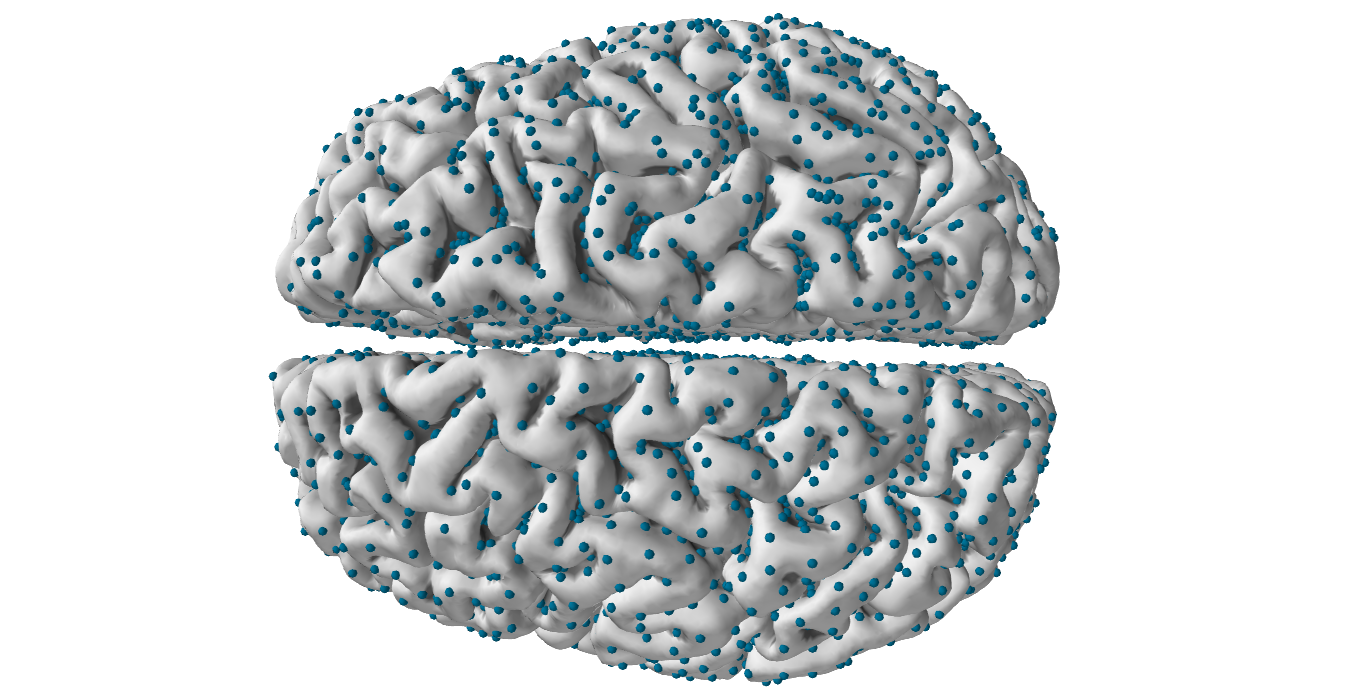
\includegraphics[scale=0.3]{../images/brain.png}
\caption{Пример сетки в пространстве источников,
          построенной на основе трехмерной анатомической модели}
\label{fig:src_space}
\end{figure}

\begin{equation}
    \mathbf{x}_k(t) = \mathbf{G} \cdot \mathbf{s}_k(t) + \mathbf{\omega}_k(t),
    \label{gm_ts}
\end{equation}
где $\mathbf{s}_k(t)$ --- $n$-мерный вектор-столбец активаций источников,
$\mathbf{x}_k(t)$ --- $m$-мерный вектор-столбец сигналов на сенсорах,
$t$ --- время, а $\mathbf{G}$ --- $m \times n$ матрица линейного отображения пространства источников в пространство сенсоров.
Индекс $k$ обозначает номер эпохи.
Применим к (\ref{gm_ts}) частотное преобразование. Существует много способов произвести
эту операцию, например, --- вейвлет-преобразование или узкополосная фильтрация
с последующим аналитическим представлением сигнала.
Мы не будем вдаваться в подробности теории частотно-временных преобразований;
для подробного математизированного изложения предмета см.
\cite{Oppenheim1998}, о  применении  частотно-временных преобразований к обработке
электрофизиологических данных можно прочитать в \cite{Freeman}.
Мы только упомянем, что вне зависимости от особенностей выбранного
метода образом частотно-временного преобразования матрицы $\mathbf{X}$ размера $m \times T$
будет комплексный тензор, каждый временной срез которого содержит в себе информацию
о фазовом и амплитудном спектре сигнала в каждый момент времени.
Чтобы упростить вывод, мы зафиксируем одну частоту имея в виду,
что дальнейшие выкладки справедливы и для остальных частот преобразования. В итоге мы можем записать:

\begin{equation}
    \hat{\mathbf{x}}_{k,f_i}(t) = \mathbf{G} \cdot \hat{\mathbf{s}}_{k,f_i}(t) + \hat{\mathbf{\omega}}_{k,f_i}(t),
    \label{gm_timefreq}
\end{equation}
где $\hat{\mathbf{x}}, \hat{\mathbf{s}}, \hat{\mathbf{\omega}}$ --- комплекснозначные образы $\mathbf{x}, \mathbf{s}, \mathbf{\omega}$ соответственно.
Для простоты далее будем опускать нижний индекс $f_i$:

\begin{equation}
    \hat{\mathbf{x}}_k(t) = \mathbf{G} \cdot \hat{\mathbf{s}}_k(t) + \hat{\mathbf{\omega}}_k(t)
    \label{gm_timefreq_no_fi}
\end{equation}

Теперь, если мы для каждой эпохи умножим $\hat{\mathbf{x}}_k(t)$ на его эрмитово сопряжение и усредним результат,
мы получим порождающую модель кросс-спектра на сенсорах:

\begin{gather}
           \langle{\hat{\mathbf{x     }}_k(t) \hat{\mathbf{x}}_k(t)^{\dag}} \rangle_{k=1}^K =
           \langle{(\mathbf{G} \cdot\hat{\mathbf{s}}_k(t) + \hat{\mathbf{\omega}}_k(t))
                                       (\mathbf{G} \cdot\hat{\mathbf{s}}_k(t) + \hat{\mathbf{\omega}}_k(t))^{\dag}}\rangle_{k=1}^K=\nonumber\\
= \mathbf{G}  \cdot \langle{\hat{\mathbf{s     }}_k(t) \hat{\mathbf{s     }}_k(t)^{\dag}} \rangle_{k=1}^K \cdot \mathbf{G}^T +
   \mathbf{G} \cdot \langle{\hat{\mathbf{s     }}_k(t) \hat{\mathbf{\omega}}_k(t)^{\dag}} \rangle_{k=1}^K + \nonumber\\
        +  \langle{\hat{\mathbf{\omega}}_k(t) \hat{\mathbf{s     }}_k(t)^{\dag}} \rangle_{k=1}^K \cdot \mathbf{G}^T +
           \langle{\hat{\mathbf{\omega}}_k(t) \hat{\mathbf{\omega}}_k(t)^{\dag}} \rangle_{k=1}^K,
    \label{gm_cp_ini}
\end{gather}
\\
где оператор $\langle \cdot \rangle_{k=1}^K$ означает усреднение по эпохам.

Так как шум предполагается белым, а сигнал на сенсорах $\hat{\mathbf{s}}_k$ и шум $\hat{\mathbf{\omega}}_k$ взаимно независимыми,
можем заметить, что второй и третий члены уравнения (\ref{gm_cp_ini}) равны нулю, когда число эпох достаточно велико.
Также отметим, что
$\hat{\mathbf{x     }}_k(t) \hat{\mathbf{x     }}_k(t)^{\dag}$,
$\hat{\mathbf{s     }}_k(t) \hat{\mathbf{s     }}_k(t)^{\dag}$ и
$\hat{\mathbf{\omega}}_k(t) \hat{\mathbf{\omega}}_k(t)^{\dag}$
представляют собой внешние произведения комплексно-значных векторов на свои комплексные сопряжения,
и следовательно являются эрмитовыми матрицами, что означает,
что значения, находящиеся на диагоналях этих матриц, принадлежат к области вещественных чисел.
Это свойство, очевидно, сохраняется и после усреднения.
Более того, раз элементы векторов являются комплексными числами, они могут быть представлены в виде
$\hat{\xi}(t) = r(t)\cdot e^{i\phi(t)}$, где $\phi(t)$ соответствует мгновенной фазе сигнала,
а $r(t)$ амплитуде. Следовательно,
$\langle \hat{\xi}_p \hat{\xi}_q^* \rangle = \langle r_p r_q e^{i\Delta\phi} \rangle$ или,
если для иллюстрации мы примем, что амплитуды и фазы независимы
(справедливость последнего является предметом разногласий для электрофизиологических данных \cite{Lachaux1999}, \cite{imcoh}),
мы получим, что
$\langle \hat{\xi}_p \hat{\xi}_q^* \rangle = \langle r_p r_q \rangle \langle e^{i\Delta\phi} \rangle$.

Из последнего соотношения можно сделать несколько выводов.
Во-первых, элементы матрицы кросс-спектра представляют собой степень стабильности
разности фаз $\Delta\phi$ по эпохам.
Так, если разность фаз была достаточно равномерно распределена по всему возможному
интервалу принимаемых значений, то среднее $\langle e^{i\Delta\phi} \rangle$
будет приблизительно равно нулю.
С другой стороны, если разность фаз сохраняется от эпохи к эпохе,
результирующий коэффициент будет отличен от нуля,
что соответствует случаю установления коннективности между сигналами.
Во-вторых, если разность фаз мала,
элементы взаимного спектра могут быть близки к ненулевому вещественному числу.

Введем следующее обозначение для матрицы кросс-спектральной плотности:

\begin{equation}
    \Cp{v} \stackrel{def}{=} \langle{\hat{\mathbf{v}}_k(t) \hat{\mathbf{v}}_k(t)^{\dag}}\rangle_{k=1}^K, \\
    \label{cp_def}
\end{equation}
Используя определение (\ref{cp_def}) и опуская нулевые члены, (\ref{gm_cp_ini})
перепишется в виде
\begin{equation}
    \Cp{x}(t) = \mathbf{G} \Cp{s}(t) \mathbf{G}^T + \Cp{\omega}(t)
    \label{gm_cp_matr}
\end{equation}

Теперь рассмотрим более детально диагональ матрицы $\Cp{s}$.
Как уже было сказано, элементы главной диагонали этой матрицы являются вещественными числами
и они представляют собой значения мощностей сигналов пространства источников,
имеющих частоту $f_i$. В структуре порождающей модели отражен тот факт,
что после отображения оператором из пространства источников в пространство сенсоров
с помощью оператора $\mathbf{G}$ эти мощностные члены будут смешаны с истинной коннективностью,
и так как исходная система уравнений была сильно недоопределена (условие $n >> m$),
разделить сигналы не представляется возможным.
Математически, этим и объясняется эффект протечки сигнала.

Чтобы внести дополнительную ясность, представим себе ситуацию,
когда синхронизация между источниками полностью отсутствует,
но при этом некоторые участки мозга активны.
В такой постановке все элементы матрицы $\Cp{s}$, лежащие вне главной диагонали,
будут равны нулю, но для $\Cp{x}$ это выполняться не будет.
Пары сенсоров, расположенные близко к активным участкам мозга,
будут иметь большие кросс-спектральные коэффициенты,
что приведет к ложному обнаружению коннективности между источниками.

В ранее упомянутом методе ImCoh (в настоящее время, вероятно,
наиболее часто используемом для измерения коннективности)
предлагается рассматривать только мнимые части уравнения (\ref{gm_cp_matr}),
что уберегает нас от негативного эффекта протечки сигнала,
но при этом мы также теряем действительную часть <<хорошего>> сигнала, несущую
информацию о фазовой синхронизации.

\subsection{Проекция}

Для более полного использования информации о фазовой синхронизации, содержащейся в кросс-спектре
мы предлагаем другой подход к устранению эффекта протечки сигнала.
Распишем  произведение матриц $\mathbf{G} \Cp{s} \mathbf{G}^T$ в правой части уравнения (\ref{gm_cp_matr}):

\begin{gather}
    \Cp{x}(t) = \sum\limits_{p=1}^n\sum\limits_{q=1}^n\mathbf{g}_p\mathbf{g}_q^T c_{pq}^{\mathbf{ss}}(t) + \Cp{\omega}(t),
    \label{cp_rhs_expanded}
\end{gather}
где $\mathbf{g}_p$ --- столбец матрицы $\mathbf{G}$, который называют \emph{топографией} источника $p$,
поскольку он определяет, каким образом сигнал, поступающий от источника $p$, будет виден на сенсорах.
Можно заметить, что кросс-спектр на уровне сенсоров представляет собой взвешенную сумму внешних произведений топографий,
взятую с коэффициентами, являющимися элементами кросс-спектра из пространства источников.

\section{Произведение Кронекера}
Векторизуем уравнение (\ref{cp_rhs_expanded}):

\begin{gather}
    vec(\Cp{x}(t)) = \sum\limits_{p=1}^n\sum\limits_{q=1}^n vec(\mathbf{g}_p\mathbf{g}_q^T) c_{pq}^{\mathbf{ss}}(t) + vec(\Cp{\omega}(t))
    \label{cp_rhs_vec}
\end{gather}

Для упрощения записи будем использовать понятие произведения Кронекера.
Произведением Кронекера матриц $A$ и $B$, имеющих размеры $p\times q$ и $r\times s$ соответственно, называется матрица вида

\begin{equation}
    \mathbf{A} \otimes \mathbf{B} \stackrel{def}{=}
    \begin{bmatrix}
        a_{11} \mathbf{B} & a_{12} \mathbf{B} & \dots & a_{1n} \mathbf{B} \\
        a_{21} \mathbf{B} & a_{22} \mathbf{B} & \dots & a_{2n} \mathbf{B} \\
        \vdots            & \vdots            & \dots & \vdots            \\
        a_{m1} \mathbf{B} & a_{m2} \mathbf{B} & \dots & a_{mn} \mathbf{B}
        \label{kron_def}
     \end{bmatrix}
\end{equation}

Произведение Кронекера является билинейной ассоциативной операцией:

\begin{gather}
     \mathbf{A} \otimes (\mathbf{B} + \mathbf{C}) = \mathbf{A} \otimes \mathbf{B} + \mathbf{A} \otimes \mathbf{C} \\
    (\mathbf{A} + \mathbf{B}) \otimes \mathbf{C} = \mathbf{A} \otimes \mathbf{C} + \mathbf{B} \otimes \mathbf{C} \\
    \alpha(\mathbf{A} \otimes \mathbf{B}) = (\alpha\mathbf{A}) \otimes \mathbf{B} = \mathbf{A} \otimes (\alpha\mathbf{B}) \\
    \mathbf{A} \otimes(\mathbf{B} \otimes \mathbf{C}) =
   (\mathbf{A} \otimes \mathbf{B})\otimes \mathbf{C} =
    \mathbf{A} \otimes \mathbf{B} \otimes \mathbf{C}
\end{gather}

Заметим также, что произведение Кронекера не является симметричным: $\mathbf{A} \otimes \mathbf{B} \neq \mathbf{B} \otimes \mathbf{A}$.
Приведем другие полезные соотношения:

\begin{gather}
    (\mathbf{A} \otimes \mathbf{B})^T = \mathbf{A}^T \otimes \mathbf{B}^T \\
    (\mathbf{A} \otimes \mathbf{B}) (\mathbf{C} \otimes \mathbf{D}) = (\mathbf{A} \mathbf{B}) \otimes (\mathbf{C} \mathbf{D})
\end{gather}

Существует особо интересное для нас свойство произведения Кронекера, связывающее его с процедурой векторизации.
Для матриц $\mathbf{A}$, $\mathbf{B}$, $\mathbf{C}$ справедливо (доказательство см. в [10]):

\begin{equation}
    vec(\mathbf{A} \mathbf{B} \mathbf{C}) = (\mathbf{C}^T \otimes \mathbf{A}) vec(\mathbf{C})
\end{equation}

Отметим, что в нашем случае приведенное выражение принимает самую простую форму:

\begin{gather}
    vec[\mathbf{g}_p \mathbf{g}_q^T] = vec\left[
        \begin{pmatrix}
            g_p^1 \\
            \vdots \\
            g_p^m
        \end{pmatrix}
    \cdot 1 \cdot
    \begin{pmatrix}
        g_q^1 & \dots & g_q^m
    \end{pmatrix}
    \right] = %\nonumber \\
    \begin{pmatrix}
        g_q^1 \\
        \vdots \\
        g_q^m
    \end{pmatrix}
    \otimes
    \begin{pmatrix}
        g_p^1 \\
        \vdots \\
        g_p^m
    \end{pmatrix}
    \cdot
    vec(1) =
    \mathbf{g}_q \otimes \mathbf{g}_p,
\end{gather}

где $\mathbf{g}_q \otimes \mathbf{g}_p$ представляет собой вектор-столбец размера $m^2 \times 1$.
Перепишем выражение (\ref{cp_rhs_vec}), используя новые обозначения:

\begin{equation}
    vec(\Cp{x}(t)) = \sum\limits_{p=1}^n\sum\limits_{q=1}^n \mathbf{g}_q\otimes \mathbf{g}_p \cdot c_{pq}^{\mathbf{ss}}(t) + vec(\Cp{\omega}(t))
    \label{cp_rhs_kron}
\end{equation}
Теперь можно видеть, что векторизованный кросс-спектр на уровне сенсоров представлен линейной
комбинацией векторов $\mathbf{g}_q \otimes \mathbf{g}_p$ в $m^2$-мерном векторном пространстве.
Назовем эти векторы \emph{2-топографиями}.
Нам уже известно, что эффект протечки сигнала, от которого необходимо избавиться,
обусловлен 2-топографиями особого вида $\mathbf{g}_p \otimes \mathbf{g}_p$ (всего $n$ векторов),
конкретный вид которых нам задан через оператор $\mathbf{G}$.
Следовательно, мы можем спроецировать выражение (\ref{cp_rhs_kron}) ортогонально линейному пространству,
натянутому на 2-топографии источников протечки сигнала.

\subsection{Построение оператора проецирования}
Прежде чем мы начнем построение оператора ортогональной проекции от подпространства протечки сигнала,
необходимо понять, как соотносится подпространство протечки сигнала с линейными оболочками
2-топографий действительной и мнимой частей порождающей модели кросс-спектра на сенсорах.

Во-первых, выделим в уравнении (\ref{cp_rhs_kron}) действительную и мнимую части.
Заметим, что так как матрица $\Cp{s}$ является эрмитовой,
$c^{\mathbf{ss}}_{pq} = \overline{c^{\mathbf{ss}}_{qp}}$ (верхняя черта обозначает комплексное сопряжение):

\begin{gather}
                      \sum\limits_{p=1}^n\sum\limits_{q=1}^n \mathbf{g}_q\otimes \mathbf{g}_p \cdot c_{pq}^{\mathbf{ss}}(t) =
             Re\left(\sum\limits_{p,q=1}^{n,n} \mathbf{g}_q\otimes \mathbf{g}_p \cdot c_{pq}^{\mathbf{ss}}(t)\right) +
     i \cdot Im\left(\sum\limits_{p,q=1}^{n,n} \mathbf{g}_q\otimes \mathbf{g}_p \cdot c_{pq}^{\mathbf{ss}}(t)\right) = \nonumber \\
           = \sum\limits_{p\leq q}^{n,n} (\mathbf{g}_q\otimes \mathbf{g}_p + \mathbf{g}_p\otimes \mathbf{g}_q)
                                                                                    Re\left(c_{pq}^{\mathbf{ss}}(t)\right) +
     i \cdot \sum\limits_{p<q}^{n,n} (\mathbf{g}_q\otimes \mathbf{g}_p - \mathbf{g}_p\otimes \mathbf{g}_q)
                                                                                    Im\left(c_{pq}^{\mathbf{ss}}(t)\right)
    \label{cp_re_im}
\end{gather}

Отметим изменения в индексах суммирования.

Для удобства обозначим линейное пространство, натянутое на 2-топографии, ответственные за протечку сигнала, как
$S_{SL}$, а линейную оболочку 2-топографий мнимой части --- $S_{Im}$.

Из уравнения (\ref{cp_re_im}) видно, что 2-топографии действительной и мнимой частей устроены по-разному,
а именно, --- векторы $\mathbf{g}_q \otimes \mathbf{g}_p + \mathbf{g}_p \otimes \mathbf{g}_q$ являются симметричными,
тогда как 2-топографии мнимых частей $\mathbf{g}_q \otimes \mathbf{g}_p - \mathbf{g}_p \otimes \mathbf{g}_q$
антисимметричны по индексам $p, q$.
Нас интересует, как это структурное отличие проявляется во взаимосвязи подпространств $S_{Re}$ и $S_{Im}$ с
подпространством протечки сигнала $S_{VC}$.
Покажем, что  2-топографии мнимой части ортогональны векторам, на которые натянуто подпространство объемной проводимости:
\begin{gather}
    (\mathbf{g}_s \otimes \mathbf{g}_s)^T(\mathbf{g}_q \otimes \mathbf{g}_p - \mathbf{g}_p \otimes \mathbf{g}_q) =
        (\mathbf{g}_s^T \otimes \mathbf{g}_s^T)(\mathbf{g}_q \otimes \mathbf{g}_p) -
        (\mathbf{g}_s^T \otimes \mathbf{g}_s^T)(\mathbf{g}_p \otimes \mathbf{g}_q) = \nonumber \\
       =(\mathbf{g}_s^T \mathbf{g}_q \otimes \mathbf{g}_s^T \mathbf{g}_p -
         \mathbf{g}_s^T \mathbf{g}_p \otimes \mathbf{g}_s^T \mathbf{g}_q) \stackrel{*}{=}
        (\mathbf{g}_s^T \mathbf{g}_p \mathbf{g}_s^T \mathbf{g}_q -
         \mathbf{g}_s^T \mathbf{g}_p \mathbf{g}_s^T \mathbf{g}_q) = 0
         \label{vc_ort_im}
\end{gather}

Равенство $*$ сохраняется, так как $\mathbf{g}^T_s \mathbf{g}_q$ и $\mathbf{g}_s^T \mathbf{g}_p$ являются скалярными величинами,
и мы можем опустить операцию ``$\otimes$'' и поменять местами множители.
Из (\ref{vc_ort_im}) можно видеть,
что подпространство объемной проводимости ортогонально мнимой части подпространства.
Для действительной части такое соотношение не сохраняется:
\begin{gather}
    (\mathbf{g}_s \otimes \mathbf{g}_s)^T(\mathbf{g}_q \otimes \mathbf{g}_p + \mathbf{g}_p \otimes \mathbf{g}_q) =
        (\mathbf{g}_s^T \otimes \mathbf{g}_s^T)(\mathbf{g}_q \otimes \mathbf{g}_p) +
        (\mathbf{g}_s^T \otimes \mathbf{g}_s^T)(\mathbf{g}_p \otimes \mathbf{g}_q) = \nonumber \\
       =(\mathbf{g}_s^T \mathbf{g}_q \otimes \mathbf{g}_s^T \mathbf{g}_p +
         \mathbf{g}_s^T \mathbf{g}_p \otimes \mathbf{g}_s^T \mathbf{g}_q) =
        2\langle\mathbf{g}_s, \mathbf{g}_p\rangle \langle\mathbf{g}_s, \mathbf{g}_q\rangle
         \label{vc_ort_re}
\end{gather}

После проведенных операций легко увидеть, что проекция ортогонально подпространству протечки сигнала
оказывает влияние на подпространство действительной части кросс-спектра на источниках.
Следовательно, нужно добиться того, чтобы протечка сигнала была удалена из данных
насколько это возможно с учетом минимального воздействия на подпространство
действительной части кросс-спектра (см.рис.~\ref{fig:subspaces}).
Для достижения этой цели необходимо уменьшить размерность подпространства
объемной проводимости неким оптимальным способом.

\begin{figure}[htbp]
\centering
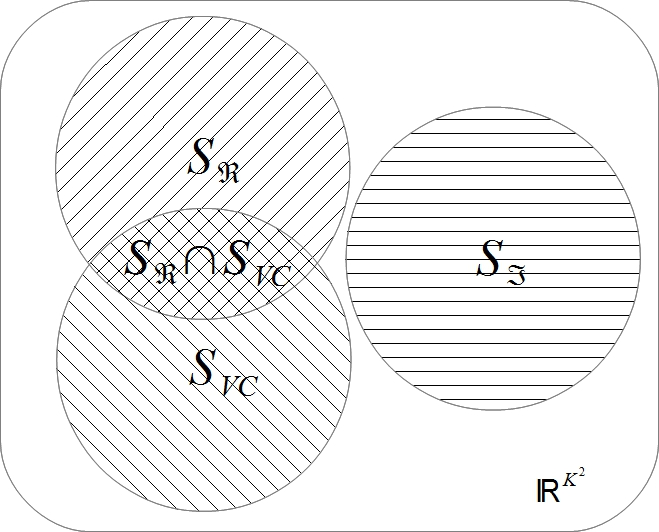
\includegraphics[width=12cm]{./images/SetsReImVC.jpg}
\caption{Взаимосвязь подпространств для кросс-спектра на уровне сенсоров}
\medskip
\small
Подпространство протечки сигнала $S_{SL}$ и подпространство действительной части кросс-спектра $S_{\Re}$
имеют непустое пересечение. Кроме того, оба этих подпространства ортогональны подпространству мнимой
части кросс-спектра $S_{\Im}$.
Пересечение $S_{SL}$ с $S_{\Re}$ содержит вклад как от протечки сигнала,
так и от истинно взаимодействующих источников, расположенных близко друг к другу и характеризующихся малой разностью фаз.
\label{fig:subspaces}
\end{figure}%
Имея в виду все вышеперечисленное, вернемся к построению проектора.
Рассмотрим матрицу, составленную из вектор-столбцов, образующих подпространство протечки сигнала:

\begin{equation}
    \mathbf{F} =
    \begin{bmatrix}
        |                                 & |                                 &       & |                                 \\
        \mathbf{g}_1 \otimes \mathbf{g}_1 & \mathbf{g}_2 \otimes \mathbf{g}_2 & \dots & \mathbf{g}_n \otimes \mathbf{g}_n \\
        |                                 & |                                 &       & |
    \end{bmatrix}
\end{equation}

Произведем сингулярное разложение матрицы $\mathbf{F}$ \cite{Golub1996}.

\begin{equation}
    \mathbf{F} = \mathbf{USV}^T
    =
    \begin{bmatrix}
        |            & |            &        & |       \\
        \mathbf{u}_1 & \mathbf{u}_2 & \dots  & \mathbf{u}_{m^2} \\
        |            & |            &        & |
    \end{bmatrix}
    % S
    % \begin{pmatrix}
    %   \lambda_1 & 0         & \dots   & 0             & 0 & \dots & 0 \\
    %   0         & \lambda_2 & \dots   & \vdots        & 0 & \dots & 0 \\
    %   \vdots    &           & \ddots  & 0             & 0 & \dots & 0 \\
    %   0         & \dots     & \dots   & \lambda_{m^2} & 0 & \dots & 0
    % \end{pmatrix}
    \begin{pmatrix}
        \lambda_1 & 0         & \dots    \\
        0         & \lambda_2 & \dots    \\
        \vdots    &           & \ddots
    \end{pmatrix}
    % Diag(\lambda_1, \dots, \lambda_{m^2})
    \begin{bmatrix}
        - & \mathbf{v}_1 & - \\
        - & \mathbf{v}_2 & - \\
          & \dots        &   \\
        - & \mathbf{v}_n & -
    \end{bmatrix}
\end{equation}
\\
В соответствии со свойствами сингулярного разложения, первые $r$ колонок матрицы $\mathbf{U}$
образуют ортонормальный базис $r$-мерного линейного пространства, являющегося лучшим $r$-мерным приближением $n$-мерного
подпространства протечки сигнала. Используем эти $r$ векторов для построения проектора с уменьшенным рангом:

\begin{gather}
    \mathbf{U}_r =
    \begin{bmatrix}
        |            & |            &        & |       \\
        \mathbf{u}_1 & \mathbf{u}_2 & \dots  & \mathbf{u}_r \\
        |            & |            &        & |
    \end{bmatrix};\\
    \mathbf{P}_r = \mathbf{I} - \mathbf{U}_r \mathbf{U}_r^T
 \end{gather}
Итак, мы построили оператор проекции ортогонально подпространству протечки сигнала $\mathbf{P}_r$
с сокращенным рангом $r$.
Умножение уравнения (\ref{cp_rhs_kron}) на этот оператор приводит к тому, что  из порождающей
модели кросс-спектра на уровне сенсоров частично удаляются члены ответственные за эффект протечки сигнала;
параметр $r$ при этом определяет баланс между желаемым уровнем очистки от протечки сигнала и
воздействием проектора на действительную часть кросс-спектра.

Окончательно, выражение для кросс-спектра на уровне сенсоров после проекции от протечки сигнала
запишется в виде:

\begin{equation}
    vec(\Cp{x})^\perp = \mathbf{P}_r vec(\Cp{x}) =  \sum\limits_{p=1}^n\sum\limits_{q=1}^n \mathbf{P}_r \mathbf{g}_q\otimes \mathbf{g}_p \cdot c_{pq}^{\mathbf{ss}}(t) + \mathbf{P}_r vec(\Cp{\omega}(t))
    \label{cp_final}
\end{equation}

Элементы полученного таким образом векторизованного кросс-спектра $vec(\Cp{x})^\perp$ теперь могут быть
использованы для оценки коннективностей как на уровне сенсоров, так и в источниках.

\subsection{Модели со свободной ориентацией диполя}
С точки зрения анатомии каждая топография прямой модели $\mathbf{G}$
представляет собой распределение электромагнитного поля,
порождаемого так называемыми первичными токами, то есть токами,
текущими через апикальные дендриты кортикальных пирамидальных нейронов.
Так как апикальные дендриты расположены перпендикулярно к кортикальной мантии,
первичные токи по отношению к кортикальной мантии также имеют нормальную ориентацию.
Следовательно, точность прямой модели напрямую зависит от точности оценки вектора нормали
к поверхности коры, а значит и от количества точек, используемых для аппроксимации поверхности коры.
Вместе с тем, хотя современное моделирование с использованием метода магнитно-резонансной
томографии позволяет получать весьма детальную реконструкцию мозга с размером аппроксимирующих сеток
порядка нескольких сотен тысяч узлов, использование столь подробных сеток приводит к значительному
ухудшению производительности алгоритмов, работающих в пространстве источников, вследствие высоких затрат
по памяти и вычислительному времени при работе с большими массивами данных.

По этой причине использование разреженных сеток со сравнительно небольшим числом узлов стало
общепринятой практикой. Как уже отмечалось выше, недостаток такого подхода состоит в том, что
при прореживании сетки эффективная ориентация локальной нормали к коре становится неопределенной.

Неопределенность появляется из-за того, что после разрежения размер области на коре, соответствующей отдельно
взятому узлу сетки, возрастает, и так как каждая такая область характеризуется в общем случае
переменной кривизной, эффективная ориентация токового диполя, находящегося внутри отдельно взятой области аппроксимации,
будет зависеть от того, в какой именно части области находился диполь в тот или иной момент записи.

Частично справиться с этим эффектом позволяют модели, со \emph{свободной ориентацей диполя},
в которых эффективная ориентация становится дополнительным параметром, который необходимо оценить из данных~\cite{Lin2006}.

Для учета свободной ориентации следует представить топографию в точке $p$ коры в виде линейной
комбинации трех ортогональных друг к другу векторов топографии, размещенных в одной точке:
\begin{equation}
    \mathbf{g}_p = \mathbf{g}_p^x \xi + \mathbf{g}_p^y \eta + \mathbf{g}_p^z \zeta = [\mathbf{g}_p^x, \mathbf{g}_p^y, \mathbf{g}_p^z] \left(
    \begin{array}{ccc}
        \xi \\
        \eta \\
        \zeta
    \end{array}
    \right)
    \label{loose_or}
\end{equation}

В случае МЭГ измерений, так как магнитное поле от токового диполя с радиальной ориентацией вне сферического проводника равно нулю,
введенная тройка векторов может быть заменена парой диполей в плоскости, перпендикулярной радиальному направлению для каждого узла.
Следовательно, уравнение (\ref{loose_or}) перепишется для МЭГ в виде

\begin{equation}
    \mathbf{g}_p = \mathbf{g}_p^x \xi + \mathbf{g}_p^y \eta = [\mathbf{g}_p^x, \mathbf{g}_p^y] \left(
    \begin{array}{ccc}
        \xi \\
        \eta
    \end{array}
    \right)
    \label{loose_or_meg}
\end{equation}

Соответственно изменятся выражения и для 2-топографий протечки сигнала:

\begin{gather}
    \mathbf{g}_p \otimes \mathbf{g}_p = (\mathbf{g}_p^x \xi
                                      + \mathbf{g}_p^y \eta) \otimes (\mathbf{g}_p^x \xi
                                      + \mathbf{g}_p^y \eta) = \nonumber \\
                                      = \mathbf{g}_p^x \otimes \mathbf{g}_p^x \xi^2
                                      + \mathbf{g}_p^x \otimes \mathbf{g}_p^y \xi \eta
                                      + \mathbf{g}_p^y\otimes  \mathbf{g}_p^x \eta \xi
                                      + \mathbf{g}_p^y \otimes \mathbf{g}_p^y \eta^2 = \nonumber \\
                                      = [\mathbf{g}_p^x \otimes \mathbf{g}_p^x,
                                         \mathbf{g}_p^x \otimes \mathbf{g}_p^y
                                      + \mathbf{g}_p^y \otimes \mathbf{g}_p^x,
                                        \mathbf{g}_p^y \otimes \mathbf{g}_p^y]
\left( \begin{array}{ccc}
\xi^2 \\
\xi \eta \\
\eta^2
\end{array}
\right)
\end{gather}

Можно заметить, что 2-топографии объемной проводимости теперь принадлежат линейной оболочке трех векторов,
а именно --- $\mathbf{g}_p^x \otimes \mathbf{g}_p^x$, $\mathbf{g}_p^x \otimes \mathbf{g}_p^y + \mathbf{g}_p^y \otimes \mathbf{g}_p^x$ и $\mathbf{g}_p^y \otimes \mathbf{g}_p^y$.
Разумеется, представленная таким образом 2-топография протечки сигнала зависит только от параметра $\theta_p$ --- угла
между эффективной ориентацией топографии $\mathbf{g}_p$ и ее $х$-компоненты --- через $\xi = sin(\theta_p)$ и $\eta=cos(\theta_p)$:

\begin{equation*}
    \mathbf{g}_p \otimes \mathbf{g}_p =[\mathbf{g}_p^x \otimes \mathbf{g}_p^x, \mathbf{g}_p^x \otimes \mathbf{g}_p^y + \mathbf{g}_p^y \otimes \mathbf{g}_p^x, \mathbf{g}_p^y \otimes \mathbf{g}_p^y]
    \left( \begin{array}{ccc}
    cos(\theta_p)^2 \\
    cos(\theta_p) sin(\theta_p) \\
    sin(\theta_p)^2
    \end{array}
    \right)
\end{equation*}
Но это однопараметрическое семейство векторов не может быть эффективно сведено к линейному векторному
пространству с размерностью меньше 3 для построения соответствующего проектора,
а значит мы должны добавить все три 2-топографии источника $p$ в матрицу $F$:

\begin{equation}
    \mathbf{F} =
    \begin{bmatrix}
        \mathbf{g}_1^x \otimes \mathbf{g}_1^x, &
        \mathbf{g}_1^x \otimes \mathbf{g}_1^y + \mathbf{g}_1^y \otimes \mathbf{g}_1^x, &
        \mathbf{g}_2^x \otimes \mathbf{g}_2^x, &
        \dots, & \mathbf{g}_n^y \otimes \mathbf{g}_n^y \\
    \end{bmatrix}
\end{equation}

%\newpage
%========================================================================================================

\section{Ссылки} \label{sect1_2}
Сошлёмся на библиографию.
Одна ссылка: \cite[с.~54]{Sokolov}\cite[с.~36]{Gaidaenko}.
Две ссылки: \cite{Sokolov,Gaidaenko}.
Много ссылок: %\cite[с.~54]{Lermontov,Management,Borozda} % такой «фокус» вызывает biblatex warning относительно опции sortcites, потому что неясно, к какому источнику относится уточнение о страницах, а bibtex об этой проблеме даже не предупреждает
\cite{Lermontov,Management,Borozda,Marketing,Constitution,FamilyCode,Gost.7.0.53,Razumovski,Lagkueva,Pokrovski,Sirotko,Lukina,Methodology,Encyclopedia,Nasirova,Berestova,Kriger}.
И~ещё немного ссылок:
\cite{Article,Book,Booklet,Conference,Inbook,Incollection,Manual,Mastersthesis,Misc,Phdthesis,Proceedings,Techreport,Unpublished}.
\cite{medvedev2006jelektronnye, CEAT:CEAT581, doi:10.1080/01932691.2010.513279,Gosele1999161,Li2007StressAnalysis, Shoji199895,test:eisner-sample,AB_patent_Pomerantz_1968,iofis_patent1960}

%Попытка реализовать несколько ссылок на конкретные страницы для стандартной реализации:[\citenum{Sokolov}, с.~54; \citenum{Gaidaenko}, с.~36].

%Несколько источников мультицитата (только в biblatex)
%\cites[vii--x, 5, 7]{Sokolov}[v"--~x, 25, 526]{Gaidaenko} поехали дальше

Ссылки на собственные работы:~\cite{vakbib1, confbib1}

Сошлёмся на приложения: Приложение \ref{AppendixA}, Приложение \ref{AppendixB2}.

Сошлёмся на формулу: формула \eqref{eq:equation1}.

Сошлёмся на изображение: рисунок \ref{img:knuth}.

%\newpage
%============================================================================================================================

\section{Формулы} \label{sect1_3}

Благодаря пакету \textit{icomma}, \LaTeX~одинаково хорошо воспринимает в качестве десятичного разделителя и запятую ($3,1415$), и точку ($3.1415$).

\subsection{Ненумерованные одиночные формулы} \label{subsect1_3_1}

Вот так может выглядеть формула, которую необходимо вставить в строку по тексту: $x \approx \sin x$ при $x \to 0$.

А вот так выглядит ненумерованая отдельностоящая формула c подстрочными и надстрочными индексами:
\[
(x_1+x_2)^2 = x_1^2 + 2 x_1 x_2 + x_2^2
\]

При использовании дробей формулы могут получаться очень высокие:
\[
  \frac{1}{\sqrt{2}+
  \displaystyle\frac{1}{\sqrt{2}+
  \displaystyle\frac{1}{\sqrt{2}+\cdots}}}
\]

В формулах можно использовать греческие буквы:
\[
\alpha\beta\gamma\delta\epsilon\varepsilon\zeta\eta\theta\vartheta\iota\kappa\lambda\\mu\nu\xi\pi\varpi\rho\varrho\sigma\varsigma\tau\upsilon\phi\varphi\chi\psi\omega\Gamma\Delta\Theta\Lambda\Xi\Pi\Sigma\Upsilon\Phi\Psi\Omega
\]

\def\slantfrac#1#2{ \hspace{3pt}\!^{#1}\!\!\hspace{1pt}/
  \hspace{2pt}\!\!_{#2}\!\hspace{3pt}
} %Макрос для красивых дробей в строчку (например, 1/2)
Для красивых дробей (например, в индексах) можно добавить макрос
\verb+\slantfrac+ и писать $\slantfrac{1}{2}$ вместо $1/2$.
%\newpage
%============================================================================================================================

\subsection{Ненумерованные многострочные формулы} \label{subsect1_3_2}

Вот так можно написать две формулы, не нумеруя их, чтобы знаки равно были строго друг под другом:
\begin{align}
  f_W & =  \min \left( 1, \max \left( 0, \frac{W_{soil} / W_{max}}{W_{crit}} \right)  \right), \nonumber \\
  f_T & =  \min \left( 1, \max \left( 0, \frac{T_s / T_{melt}}{T_{crit}} \right)  \right), \nonumber
\end{align}

Выровнять систему ещё и по переменной $ x $ можно, используя окружение \verb|alignedat| из пакета \verb|amsmath|. Вот так:
\[
    |x| = \left\{
    \begin{alignedat}{2}
        &&x, \quad &\text{eсли } x\geqslant 0 \\
        &-&x, \quad & \text{eсли } x<0
    \end{alignedat}
    \right.
\]
Здесь первый амперсанд (в исходном \LaTeX\ описании формулы) означает выравнивание по~левому краю,
второй "--- по~$ x $, а~третий "--- по~слову <<если>>. Команда \verb|\quad| делает большой горизонтальный пробел.

Ещё вариант:
\[
    |x|=
    \begin{cases}
    \phantom{-}x, \text{если } x \geqslant 0 \\
    -x, \text{если } x<0
    \end{cases}
\]

Кроме того, для  нумерованых формул \verb|alignedat|  делает вертикальное
выравнивание номера формулы по центру формулы. Например,  выравнивание компонент вектора:
\begin{equation}
 \label{eq:2p3}
 \begin{alignedat}{2}
{\mathbf{N}}_{o1n}^{(j)} = \,{\sin} \phi\,n\!\left(n+1\right)
         {\sin}\theta\,
         \pi_n\!\left({\cos} \theta\right)
         \frac{
               z_n^{(j)}\!\left( \rho \right)
              }{\rho}\,
           &{\boldsymbol{\hat{\mathrm e}}}_{r}\,+   \\
+\,
{\sin} \phi\,
         \tau_n\!\left({\cos} \theta\right)
         \frac{
            \left[\rho z_n^{(j)}\!\left( \rho \right)\right]'
              }{\rho}\,
            &{\boldsymbol{\hat{\mathrm e}}}_{\theta}\,+   \\
+\,
{\cos} \phi\,
         \pi_n\!\left({\cos} \theta\right)
         \frac{
            \left[\rho z_n^{(j)}\!\left( \rho \right)\right]'
              }{\rho}\,
            &{\boldsymbol{\hat{\mathrm e}}}_{\phi}\:.
\end{alignedat}
\end{equation}

Ещё об отступах. Иногда для лучшей <<читаемости>> формул полезно
немного исправить стандартные интервалы \LaTeX\ с учётом логической
структуры самой формулы. Например в формуле~\ref{eq:2p3} добавлен
небольшой отступ \verb+\,+ между основными сомножителями, ниже
результат применения всех вариантов отступа:
\begin{align*}
\backslash! &\quad f(x) = x^2\! +3x\! +2 \\
  \mbox{по-умолчанию} &\quad f(x) = x^2+3x+2 \\
\backslash, &\quad f(x) = x^2\, +3x\, +2 \\
\backslash{:} &\quad f(x) = x^2\: +3x\: +2 \\
\backslash; &\quad f(x) = x^2\; +3x\; +2 \\
\backslash \mbox{space} &\quad f(x) = x^2\ +3x\ +2 \\
\backslash \mbox{quad} &\quad f(x) = x^2\quad +3x\quad +2 \\
\backslash \mbox{qquad} &\quad f(x) = x^2\qquad +3x\qquad +2
\end{align*}


Можно использовать разные математические алфавиты:
\begin{align}
\mathcal{ABCDEFGHIJKLMNOPQRSTUVWXYZ} \nonumber \\
\mathfrak{ABCDEFGHIJKLMNOPQRSTUVWXYZ} \nonumber \\
\mathbb{ABCDEFGHIJKLMNOPQRSTUVWXYZ} \nonumber
\end{align}

Посмотрим на систему уравнений на примере аттрактора Лоренца:

\[
\left\{
  \begin{array}{rl}
    \dot x = & \sigma (y-x) \\
    \dot y = & x (r - z) - y \\
    \dot z = & xy - bz
  \end{array}
\right.
\]

А для вёрстки матриц удобно использовать многоточия:
\[
\left(
  \begin{array}{ccc}
    a_{11} & \ldots & a_{1n} \\
    \vdots & \ddots & \vdots \\
    a_{n1} & \ldots & a_{nn} \\
  \end{array}
\right)
\]


%\newpage
%============================================================================================================================
\subsection{Нумерованные формулы} \label{subsect1_3_3}

А вот так пишется нумерованая формула:
\begin{equation}
  \label{eq:equation1}
  e = \lim_{n \to \infty} \left( 1+\frac{1}{n} \right) ^n
\end{equation}

Нумерованых формул может быть несколько:
\begin{equation}
  \label{eq:equation2}
  \lim_{n \to \infty} \sum_{k=1}^n \frac{1}{k^2} = \frac{\pi^2}{6}
\end{equation}

Впоследствии на формулы (\ref{eq:equation1}) и (\ref{eq:equation2}) можно ссылаться.

Сделать так, чтобы номер формулы стоял напротив средней строки, можно, используя окружение \verb|multlined| (пакет \verb|mathtools|) вместо \verb|multline| внутри окружения \verb|equation|. Вот так:
\begin{equation} % \tag{S} % tag - вписывает свой текст
  \label{eq:equation3}
    \begin{multlined}
        1+ 2+3+4+5+6+7+\dots + \\
        + 50+51+52+53+54+55+56+57 + \dots + \\
        + 96+97+98+99+100=5050
    \end{multlined}
\end{equation}

Используя команду \verb|\labelcref| из пакета \verb|cleveref|, можно
красиво ссылаться сразу на несколько формул
(\labelcref{eq:equation1,eq:equation3,eq:equation2}), даже перепутав
порядок ссылок \verb|(\labelcref{eq:equation1,eq:equation3,eq:equation2})|.

           % Глава 1
\chapter{Решение обратной задачи в пространстве матриц кросс-спектральной плотности} \label{chapt2}

% План.
% Методы решения обратной задачи для МЭГ/ЭЭГ.
% Сканирующий подход. Нахождение ориентации диполя.
% MUSIC, RAP-MUSIC, бимформеры. Сканирующие методы решения обратной задачи для анализа коннективностей.
% Алгоритм DICS. Модификация DICS для оценки imcoh в пр-ве источников. Wedge MUSIC.
% Методы глолбальной оптимизации.
% Оценка активностей при помощи псевдообратной матрицы.
% Априорная информация о структуре решения. MNE, MinimumCurrent, mxNormMNE.
% Адаптация MxNormMNE к решению обратной задачи для поиска синхронностей.
% Техники ускорения расчета и оптимизации вычислительных ресурсов.
% Active set и связь с MUSIC.
% Критерий останова алгоритма.
% Сокращение размерности пр-ва сенсоров.

\section{Введение}

В предыдущей главе нами была получена система уравнений, связывающая коэффициенты матрицы
кросс-спектральной плотности мощности в пространстве источников с аналогичными коэффициентами в
пространстве сенсоров. Хотя это уравнение и является линейными относительно неизвестных
величин $c_{ij}^{ss}$, процедура нахождения решения, которое адекватно описывало бы
поведение реальных систем, осложнено тем фактом, что рассматриваемая система уравнений
существенно недоопределена, а следовательно для нее существует бесконечное количество решений,
далеко не все из которых осуществимы для реальных систем взаимодействующих нейронных ансамблей.

Вообще, система уравнений \ref{eq:cp_final_re_im} для фиксированных ориентаций диполей
по своей структуре ничем кроме шумового слагаемого не отличается от систем \ref{eq:BV_generative_matrix}.
Системы уравнений \ref{eq:BV_generative_matrix} на неизвестные величины $\mathcal{Q}$ также является
линейным и недоопределенными. Некоторые отличия возникают лишь при рассмотрении свободно ориентированных диполей.

Задачу оценки величин, положений и ориентаций токовых диполей $\mathcal{Q}$
на основании измерений $\mathcal{B}, \mathcal{V}$ в электрофизиологии принятно называть \emph{обратной задачей} МЭГ/ЭЭГ.
Как и в случае оценки кросс-спектральных коэффициентов, решение обратной задачи МЭГ/ЭЭГ не единственно.
Для выбора какого-либо одного решения $\mathcal{Q}$ по коре применяют различные эвристики,
ограничивающие выбор из бесконечного множества возможных вариантов.
Как правило, получающееся решение отвечает тому или иному критерию оптимальности в соответствии с используемой эвристикой,
при условии, что предположения модели выполняются.
Во введении к этой главе мы рассмотрим основные методы решения обратной задачи для поиска
активных токовых диполей на коре, а затем перейдем к рассмотрению методик для оценки
кросс-спектральных коэффициентов с учетом свободной ориентации.

Все существующие методики решения обратной задачи МЭГ/ЭЭГ можно условно разделить на два класса.
К первому классу относятся алгоритмы, основанные на методах оптимальной фильтрации.
Суть этого подхода состоит в том, что для фиксированной точки внутри объема мозга ставится задача нахождения
пространственного фильтра, оптимизирующего определенную характеристику сигнала,
восстанавливаемого при помози этого фильтра.
В качестве такой характеристики может выступать, например, отношение сигнал/шум,
или же мы можем руководствоваться критерием минимизации протечки сигнала от других источников в точку,
в которой мы хотим восстановить активность.
Здесь важно отметить, что конкретный вид решения, полученного в результате оптимизации выбранного
функционала качества будет зависить также от предполагаемой пространственной структуры шума.

Отметим, что структура восстановленной после применения совокупности найденных фильтров
активации на коре при таком подходе, вообще говоря, субоптимальна с точки зрения объяснения сигнала,
измеренного сенсорами (так как мы оптимизировали другой функционал качества).
Проблема недоопределенности системы уравнений при этом в некотором смысле остается за скобками,
так как для каждой точки коры решение восстанавливается индивидуально ---
без учета вклада в решение активаций, восстановленных в других точках коры.
Таким образом, для первого класса алгоритмов решения обратной задачи найденное решение
является оптимальным в локальном, но не в глобальном смысле.

Задача отыскания активаций, наилучшим образом объясняющих измерения, (т.е. оптимальных в глобальном смысле)
ставится для вторго класса алгоритмов решения обратной задачи.
При этом, как уже было отмечено выше, в силу недоопределенности системы линейных уравнений,
связывающих активации на коре с сигналом на сенсорах, существует бесконечное множество
конфигураций источников, идеально объясняющих померенный сигнал.
Тем не менее, среди таких решений в силу зашумленности измерений а также неточностей
при построении прямой модели реальное распределение активаций в выделенных точках коры
не содержится, так эти <<идеальные>> с точки зрения объяснения измерений решения объясняют в том числе и
шумовую компоненту, которая зачастую оказывается больше или сравнима по амплитуде с истинной активацией.

Итак, при решении обратной задачи методами глобальной оптимизации существует две проблемы:
бесконечное множество возможных решений и зашумленность измерений. Чтобы справиться с первой проблемой,
для выбора из бесконечного множества решений пользуются критерием минимальности нормы решения.
Иными словами, среди всех возможных конфигураций первичных токов в объеме (или на поверхности коры) мозга
в качестве решения выбирается такая конфигурация, норма которой минимальна среди всех возможных.
Выбор нормы при этом определяет структуру решения.
Наиболее популярными вариантами являются $L_2$- и $L_1$-нормы.
В случае, если проблему зашумленности данных мы оставляем без внимания, решение, соответствующее
минимуму $L_2$-нормы, получается применением оператора,
соответствующего псевдообратной матрице матрицы прямой модели.



\subsection{Сканирующие алгоритмы} \label{sect_dics}
Сущестувует множество различных подходов к решению обратной задачи МЭГ/ЭЭГ, основанных
на принципиально различных идеях.
Тем не менее, задача каждой из возможных методик состоит в отыскании
линейного обратного оператора, подействовав которым на вектор значений сигнала на сенсорах
в какой-либо момент времени мы получим распределение активности по всей коре или в какой-то ее части.
При этом, полученное решение должно отвечать критерию оптимальности в том или ином смысле.

Мы начнем рассмотрение существующих методик решения обратной задачи с класса алгоритмов, которые
можно условно назвать \emph{сканирующими}. Смысл названия кроется в том,
           % Глава 2
% \chapter{Анализ свойств метода оценки синхронизации с нулевым фазовым сдвигом.}~\label{chapt3}
В этой главе мы исследуем свойства методов, основанных на проекции от протечки сигнала,
а также сравним результаты их работы с методами, являющимися на данный
момент стандартом в области исследований функциональной коннективности.

Начнем с исследования свойств базовой процедуры, описанной в разделе~\ref{sec:psiicos}.
\section{Исследование воспроизводимости решения для метода PSIICOS.}\label{sec:bootstrap}

Для проверки стабильности решений мы использовали процедуру бутстрэпа, аналогичную
описанной в~\cite{Darvas2005}.
Мы генерировали $B$ различных кросс-спектральных временных рядов (CT), полученных
усредненем по эпохам, индексы которых берутся как сочетания с повторениями, набранные
с равными вероятностями из полного набора индексов.

Затем на каждой итерации бутстрэпа небольшое
число пар $m$, соответствующих сетям с наибольшими
значениями кросс-спектральных коэффициентов, полученными в результате применения
алгоритма PSIICOS, группировались в несколько кластеров в соответствии с процедурой
попарной пространственной кластеризации (Pairwise Spatial Clustering,~\cite{Zalesky2012}).

Для каждого полученного кластера мы рассчитывали среднюю сеть. Для этого мы усредняли
координаты начал и концов сетей в кластере, предварительно ориентируя их таким
образом, чтобы концы были направлены в одну полуплоскость.
Средние сети, полученных на каждом шаге бутстрэпа, сохранялись.

Для количественной оценки пространственного разброса полученных таким образом средних сетей
мы определяли расстояние между парой сетей как минимум по двум возможным ориентациям
сетей от суммы евклидовых расстояний между их концами.

В соответствии с определенной таким образом функцией расстояния мы определяли индекс
воспроизводимости $\eta$ как единицу, деленную на среднее по всем $B$ средним сетям расстояние
от сети до ближайшего соседа.

\section{Симуляции методом Монте-Карло.}\label{sec:monte_carlo_simulation}
Чтобы сравнить предложенный алгоритм с другими методами, оценивающими коннективность
в пространстве источников, мы сконструировали ряд реалистичных симуляций.

Для симуляций использовали поверхность коры реального испытуемого,
реконструированную по МРТ-снимкам при помощи пакета программ Freesurfer.
Для аппроксимации этой поверхности трехмерной вычислительной сеткой мы
использовали 15000 узлов. Для этой поверхности мы рассчитали матрицу прямой модели
высокого разрешения $\matr{G}^{HR}$, в которой на каждую точку коры приходится
две топографии, соответствующие модели со свободной ориентацией диполя для МЭГ
в случае сферической симметрии. Эти топографии мы рассчитывали при помощи метода главных
компонент для $M \times 3$ прямой модели для отдельно взятой точки, выкидывая
компоненту с наименьшим собственным числом.

Мы симулировали 100 повторений (эпох) эксперимента, в котором за стимулом следовал
всплеск индуцированной активности на частоте 10 Гц. Индуцированная активность
симулировалась как пары синусоид, не привязанные по фазе к стимулу, но с неслучайной
разностью фаз по отношению друг к другу. Их разность фаз $\delta\phi$ выбиралась
для каждой эпохи случайно из равномерного распределения на отрезке $[-\pi/4, \pi/4]$.

Шум мозга мы моделировали как $Q=1000$ кортикальных источников, активность которых
никак не связана со стимулом. Положения на коре этих источников
выбирались для каждой эпохи независимо и случайно.

Для моделирования их временных профилей активации мы фильтровали реализации гауссовского
случайного процесса полосовым БИХ-фильтром пятого порядка в полосах частот,
соответствующих тета (4--7 Гц), альфа (8--12 Гц), бета (15--30 Гц) и гамма (30--50, 50--70 Гц)
активности. Относительные вклады этих полос частот мы взвешивали таким образом, чтобы
итоговая спектральная плотность мощности имела вид $1/f$, соответствующий реалистичному
спектру данных МЭГ. Далее общий вклад шума мозга в итоговый сигнал взвешивался,
чтобы соответствовать типичным соотношениям сигнал-шум, наблюдаемым в реальных
записях.

Для отображения шумовых источнков на сенсоры умножали каждый срез полученных временных
профилей на соответствующие столбцы матрицы $\matr{G}^{HR}$ и складывали результаты.

ОСШ в симуляционных данных мы определяли как отношение фробениусовских
норм матрицы данных и матрицы шума, отфильтрованных в целевой полосе (8--12 Гц).

Для вычисления матрицы кросс-спектральной плотности на сенсорах, соответствующей целевой полосе,
мы проводили следующую процедуру.
Мы фильтровали симулированный сигнал на каждом сенсоре в диапазоне (8--12 Гц) и
вычисляли аналитический сигнал.
Затем для каждого временного среза мы брали внешние произведения с сопряжением
комплекснозначного вектора аналитических сигналов на сенсорах и усредняли их по эпохам.

Чтобы наши симуляции были больше приближены к реальным условиям, когда настоящие источники
не всегда точно ложатся на узлы вычислительной сетки, мы использовали сетку с высоким
разрешением (15000 узлов) только для симуляции данных. Для оценки
коннективности по симуляционным данным мы использовали в 10 раз более разреженную сетку,
насчитывающую 1503 узла.

В качестве метрик качества мы использовали кривые Receiver Operating Characteristics (ROC)
и Precision-Recall (PR). Метрика Precision-Recall лучше работает в ситуации, когда
число истинно положительных мало по сравнению с общим количеством вариантов.
ROC-кривая, или график \emph{чувствительность~--- 1 - специфчность} в этом случае информативна
только для очень высоких значений специфичности.

Для каждой реализации метода Монте-Карло мы считали ROC-кривую и затем
усредняли кривые по ансамблю из 1000 реализаций. Сравнения проводились для двух различных
значений ОСШ: 1 и 0.2. 

Так как целевой характеристикой предложенного метода является одинаковое качество
решений для произвольных фазовых задержек между связанными источниками, мы сравнивали
поведение методов для двух различных фазовых задержек $\delta\phi=\pi/2-\pi/20$ и
$\delta\phi=\pi/20$ радиан. Также мы исследовали поведение нашего метода на
равномерной сетке средних значений фазового сдвига.

Для первого теста мы моделировали одну пару взаимодействующих источников. Для каждой эпохи
узлы этой сети мы располагали в двух случайно выбранных точках на сетке с высоким разрешением.
Для оценки изменяемой временной активности таких сетей на каждой эпохе мы умножали временной
профиль активации на временное окно, соответствующее активации в течение первой половины
каждой эпохи. % TODO: add ref to picture with window.

На каждой итерации процедуры Монте-Карло мы симулировали данные из 100 эпох с фиксированной
пространственной конфигурацией целевых источников и изменяющейся от эпохи к эпохе конфигурацией
источников шума мозга. Для локализации сетей мы использовали всю протяженность эпохи
чтобы смоделировать ситуацию, когда мы не знаем точно, на каком временном промежутке
сеть активна.

 \begin{figure}[!ht]
 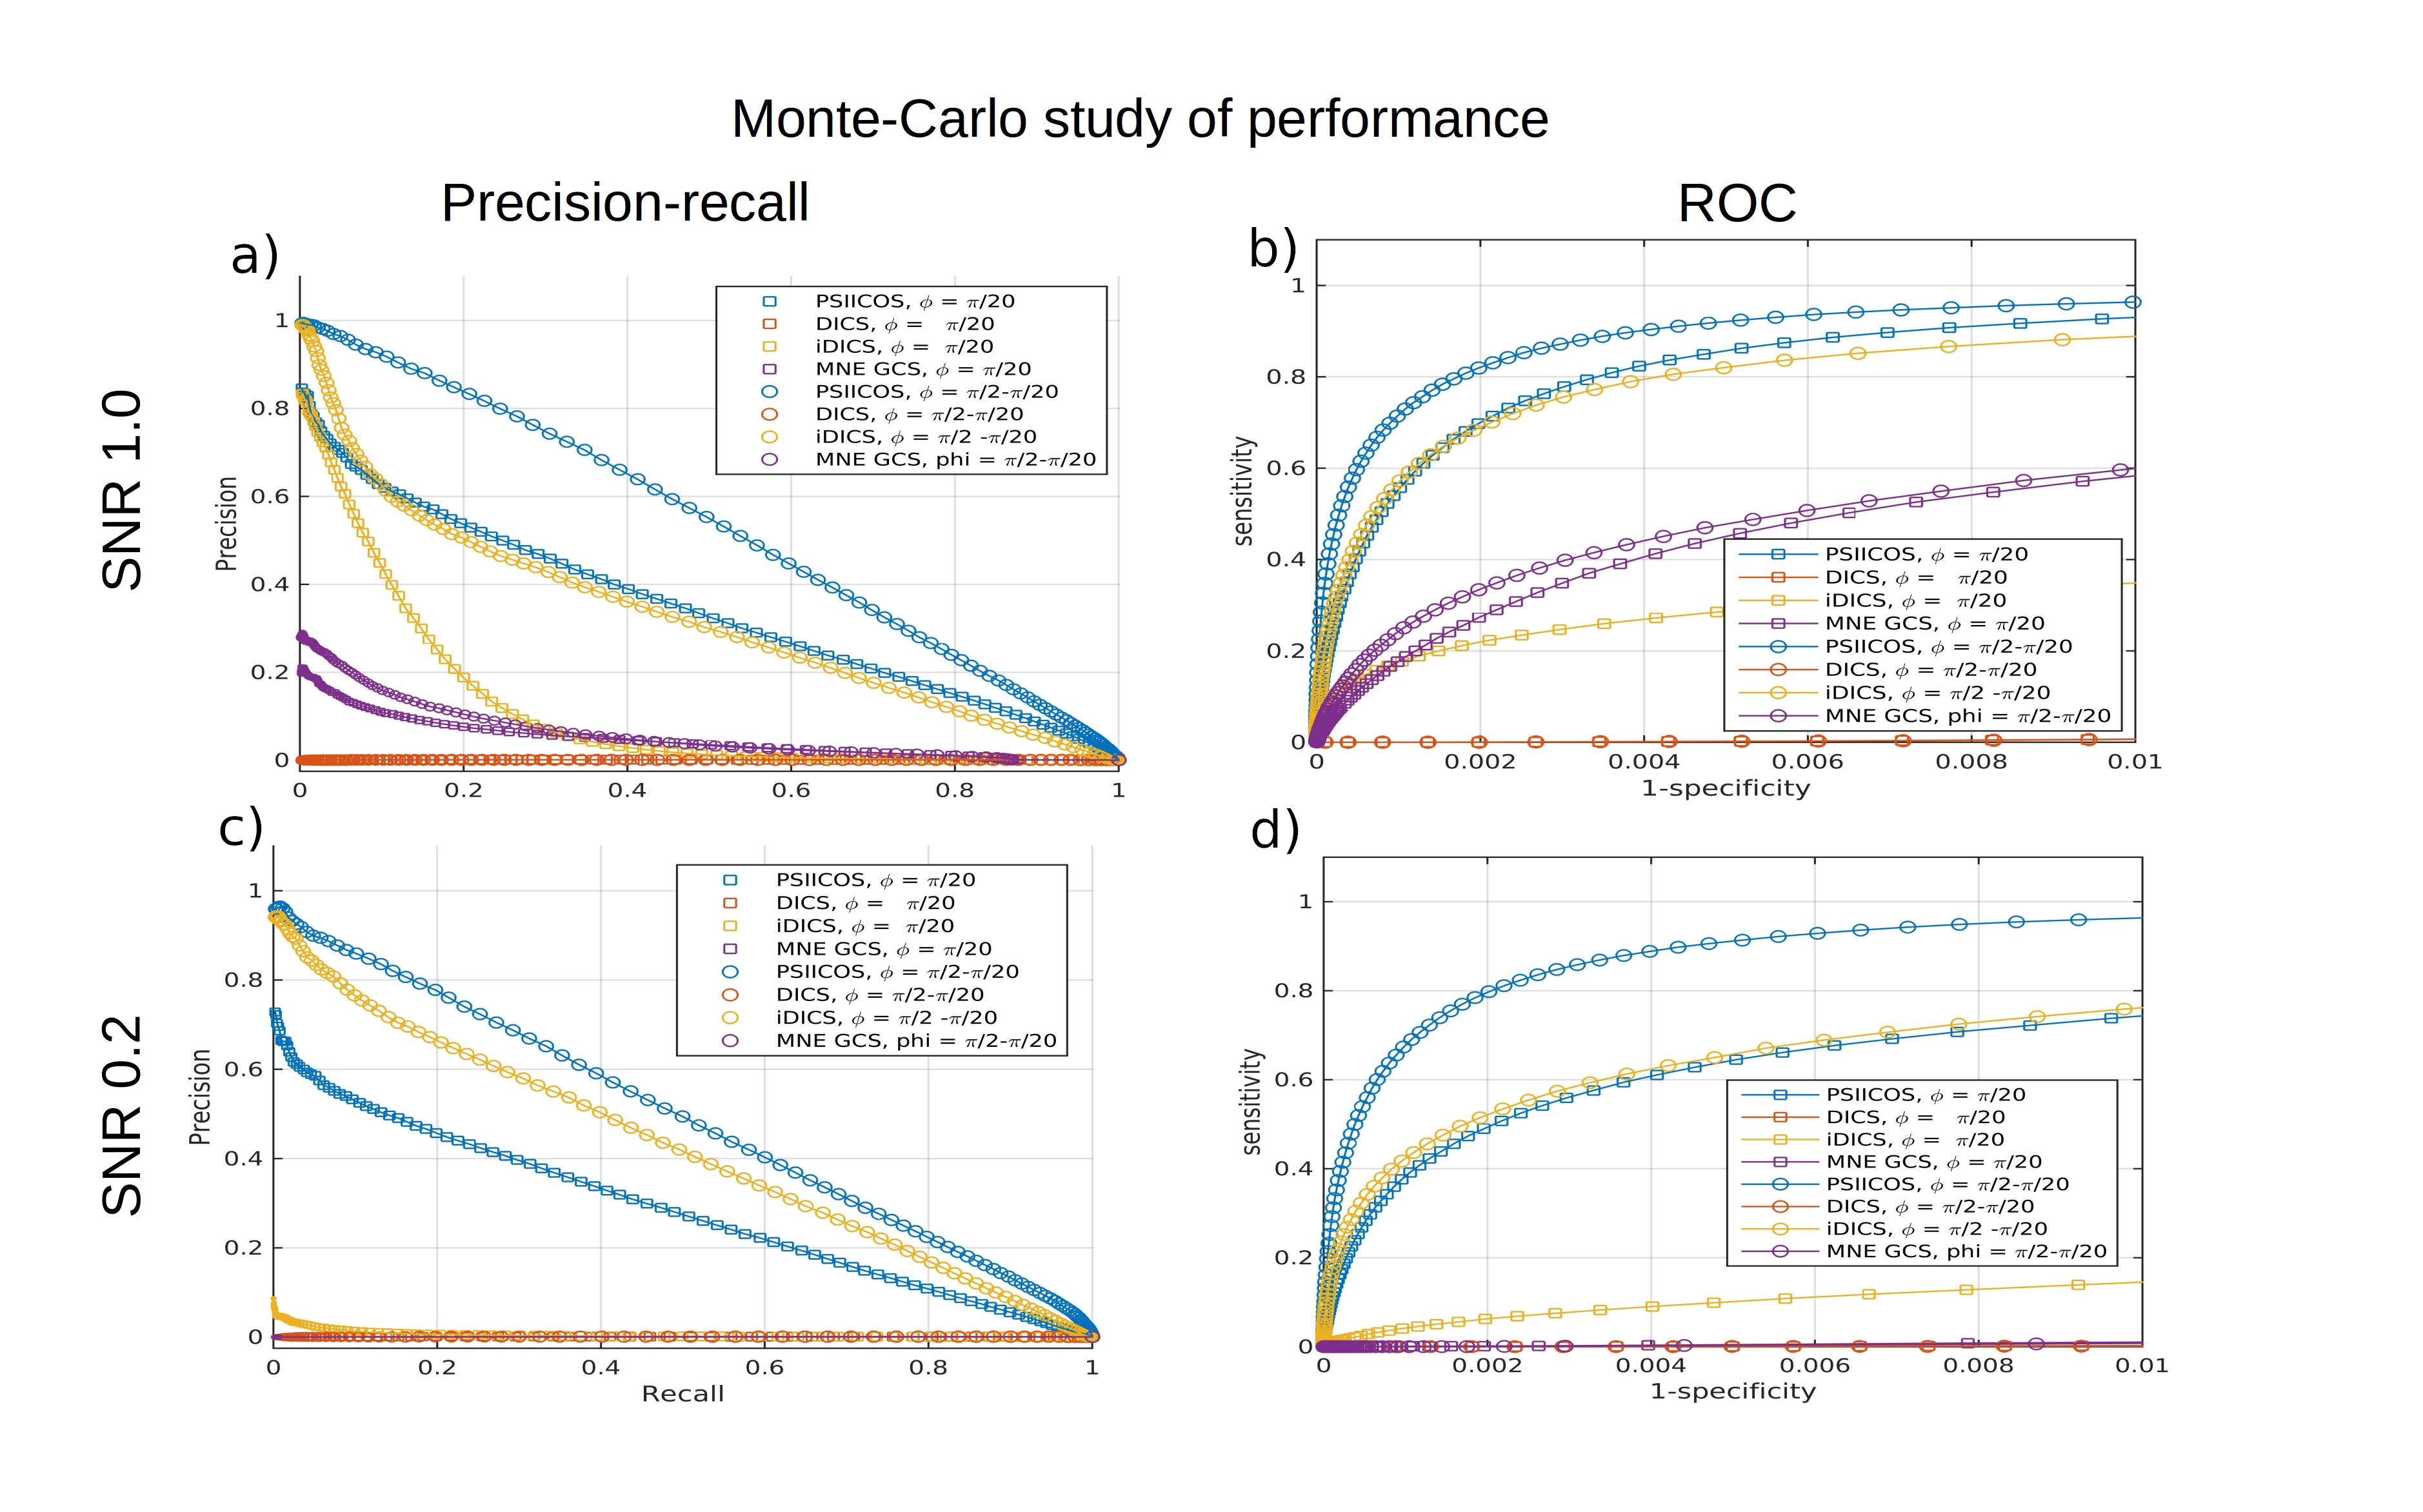
\includegraphics[width=1\textwidth]{../images/psiicos_paper/Figure4_hr_labelled_pans.jpg}
 \caption{Сравнение Precision-Recall (панели (a), (c))  и ROC- (панели (b), (d)) кривых
     в задаче локализации сетей для методов PSIICOS, DICS, iDICS и GCS MNE для
     двух значений ОСШ на основе 1000 Монте-Карло итераций.}\label{fig:04} %Figure 4
\end{figure}%

На графике~\ref{fig:04} видно, что для каждого из условий симуляции качество решений
алгоритма PSIICOS стабильно превосходит другие методы и позволяет получать решения хорошего
качества независимо от величины фазовой задержки.

По графику ROC-кривой для средней разницы фаз $\delta\phi=\pi/2 - \pi/20$ видно, что
показатели iDICS сравнимы с показателями PSIICOS.\@Однако для $\delta\phi = \pi/20$ iDICS
не способен адекватно распознавать сети в силу значительного снижения ОСШ, вызванного
тем, что сети с близкой к нулю фазовой задержкой дают очень маленький вклад во
мнимую часть кросс-спектра.

Метод MNE GCS ведет себя лучше, чем DICS для высоких значений ОСШ. Для низкого ОСШ
оба метода показывают плохие результаты. В то же время метод PSIICOS демонстрирует
адекватное качество решения для обоих значений ОСШ.

В случае низкого ОСШ большая разница в качестве решения PSIICOS между двумя
значениями фазовых задержек вероятно объясняется наличием в итерациях
Монте-Карло сетей с пространственно близкими узлами. Это приводит к тому, что
действительная часть членов, соответствующих истинному взаимодействию,
значительно искажается проекцией. Вместе с тем, остальные методы при таких
условиях для практически перестают работать в случае близких к нулю фазовых задержек.

\section{Симуляции с тремя сетями, перекрывающимися во времени.}\label{sec:three_ntw}
Для второго теста мы симулировали данные с тремя одновременно активными сетями, пространственная
и временная структура активации которых изображены на~\ref{fig:02}.
Главная сложность в этом тесте заключалась в том, чтобы разделить эти три сети в условиях
перекрывающихся окон временной активации.

\begin{figure}[htbp]
    \begin{subfigure}[t]{0.5\textwidth}
        \centering
        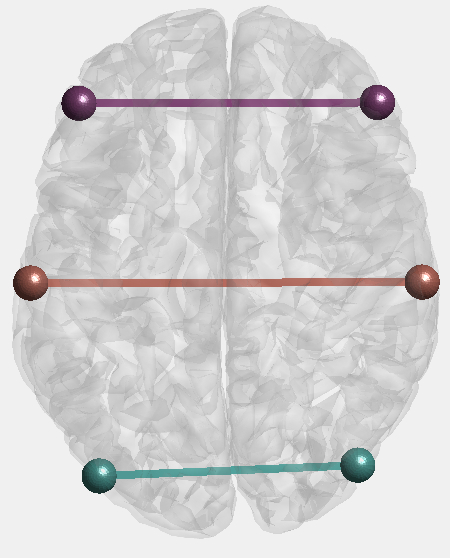
\includegraphics[angle = 90, height = 6cm]{../images/psiicos_paper/Figure2a_hr.jpg}\label{fig:2a}
        \caption{}
    \end{subfigure}
    \begin{subfigure}[t]{0.5\textwidth}
        \centering
        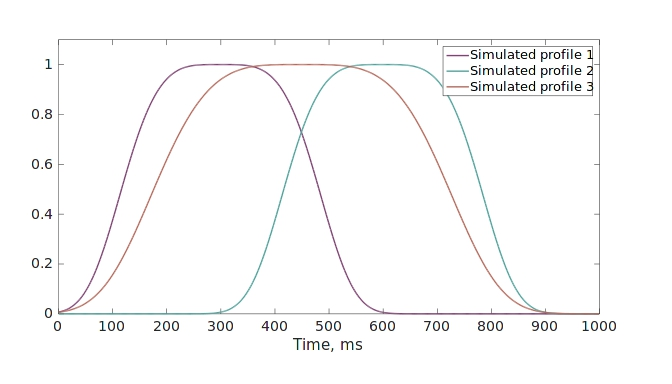
\includegraphics[width=1\textwidth]{../images/psiicos_paper/Figure2b_hr.jpg}\label{fig:2b}
        \caption{}
    \end{subfigure}
    \caption{Три симулированные пары взаимодействующих источников.}\label{02}
        (а)~--- пространственное распределение симулированных источников,
        (б)~--- временные профили активации для каждой из трех сетей.
\end{figure}


Для этих тестов мы сравнивали PSIICOS с тремя другими методами детекции
синхронных источников. Первым из этих методов был метод DICS
(см.~\ref{subsec:DICS},~\cite{Gross2001}).  При этом мы восстанавливали
элементы кросс-спектра на источниках, не нормируя их на мощность, чтобы
корректно сравнить результаты с PSIICOS.\@

Чтобы исключить влияние протечки сигнала, мы также использовали
модифицированную версию алгоритма DICS, в которой используется только мнимая
часть кросс-спектра (iDICS, см. разд.~\ref{subsec:iDICS}). Алгоритм iDICS был
вторым из набора методов, с которыми мы сравнивали PSIICOS.\@

В качестве третьего метода мы взяли алгоритм GCS~\ref{subsec:GCS}.  Как и в
оригинальной статье~\cite{Wens2015}, для построения обратного оператора мы
использовали метод MNE~\ref{subsubsec:MNE} и использовали известную матрицу
ковариации шума мозга. Алгоритму PSIICOS эта информация не нужна и поэтому не
использовалась.

На графике~\ref{fig:05} изображена пространственная структура решения для
симуляционных данных в пространстве источников. На графике отображены 0.1\% сетей
с максимальными значениями статистики, оцененной методом PSIICOS и другими тремя
алгоритмами. Как видно из графика, алгоритм PSIICOS сохраняет адекватное качество решения
для всего спектра тестируемых условий.

\begin{figure}[!ht]
 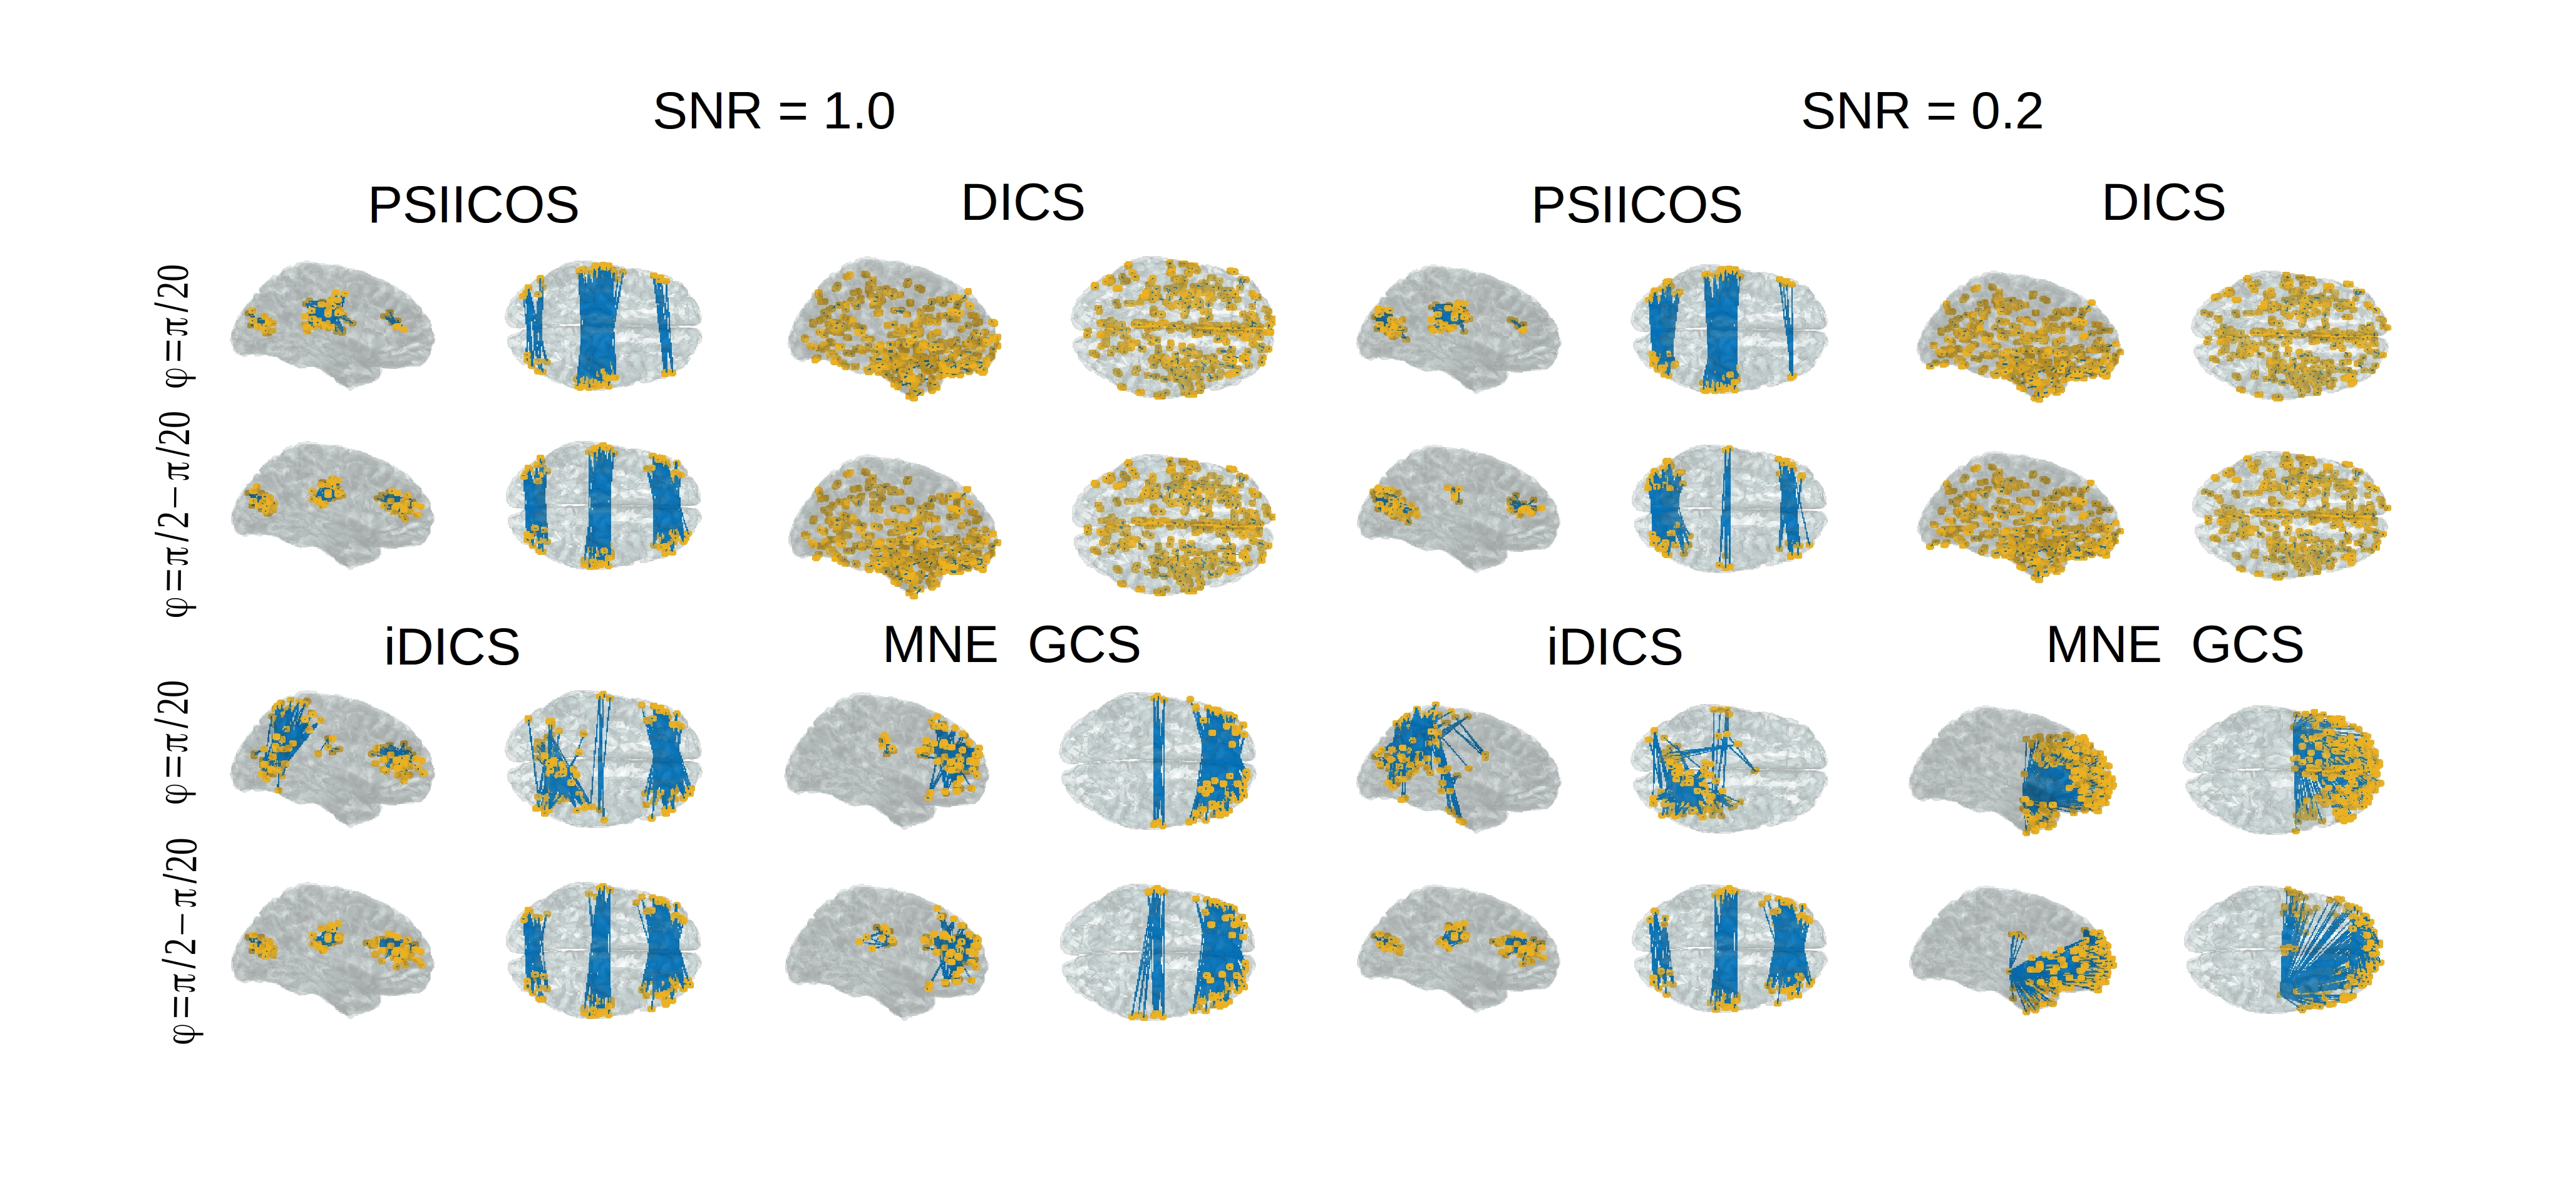
\includegraphics[width=1\textwidth]{../images/psiicos_paper/Figure5_hr.jpg}
 \caption{Пространственное распределение сетевых источников для симуляционных данных.}\label{fig:05} %Figure 5
     На графике изображены 0.1\% сетей с наибольшим значением
     статистики. Из графиков видно, что только алгоритм PSIICOS сохраняет
     качество решения для всего диапазона изучаемых значений.
     Метод iDICS ведет себя практически также хорошо, как и PSIICOS,
     для фазовых сдвигов, близких к $\pi/2$, что согласуется с нашими предыдущими
     результатами. Метод MNE GCS для высоких значений ОСШ достаточно надежно определяет
     две фронтальные сети для каждого значения фазового сдвига, но полностью перестает
     работать для низких значений ОСШ и близких к нулю фазовых задержек. Для задержек,
     близких к $\pi/2$, при низком ОСШ этот метод находит только среднюю сеть
     (для нее индивидуальное ОСШ выше всего) а также порождает большое количество
     ложноположительных срабатываний.
\end{figure}%

Как и для симуляций в разделе~\ref{sec:monte_carlo_simulation}, метод iDICS показывает себя
практически так же хорошо, как и PSIICOS для значений фазовой задержки, близких к $\pi/2$.
Метод MNE GCS для случая высокого ОСШ достаточно надежно определяет две фронтальные сети для
обоих значений фазовой задержки, но полностью перестает работать для низкого ОСШ и
околонулевой разности фаз. Для случая фазовой задержки, близкой к $\pi/2$, и низкого ОСШ
MNE GCS обнаруживает только среднюю сеть (сеть с наибольшим индивидуальным ОСШ) и
порождает большое количество ложно-положительных сетей.

Умножая временной ряд кросс-спектра на сенсорах на среднюю топографию
полученных кластеров, можем восстановить временную активность сетей.
На~\ref{fig:06} изображены временные окна, в течение которых каждая пара
взаимодействующих источников была активна.  Для построения этого графика мы
испольльзовали спроецированный от протечки сигнала временной ряд кросс-спектра,
к которому мы применяли наиболее простую процедуру оценки источников ---
фильтр, максимизирующий SNR в заданной точке~\ref{subsubsec:max_snr_filter}, с
той разницей, что здесь все операции проводились в пространстве 2-топографий с
размерностью $M^2$.

\begin{figure}[!ht]
    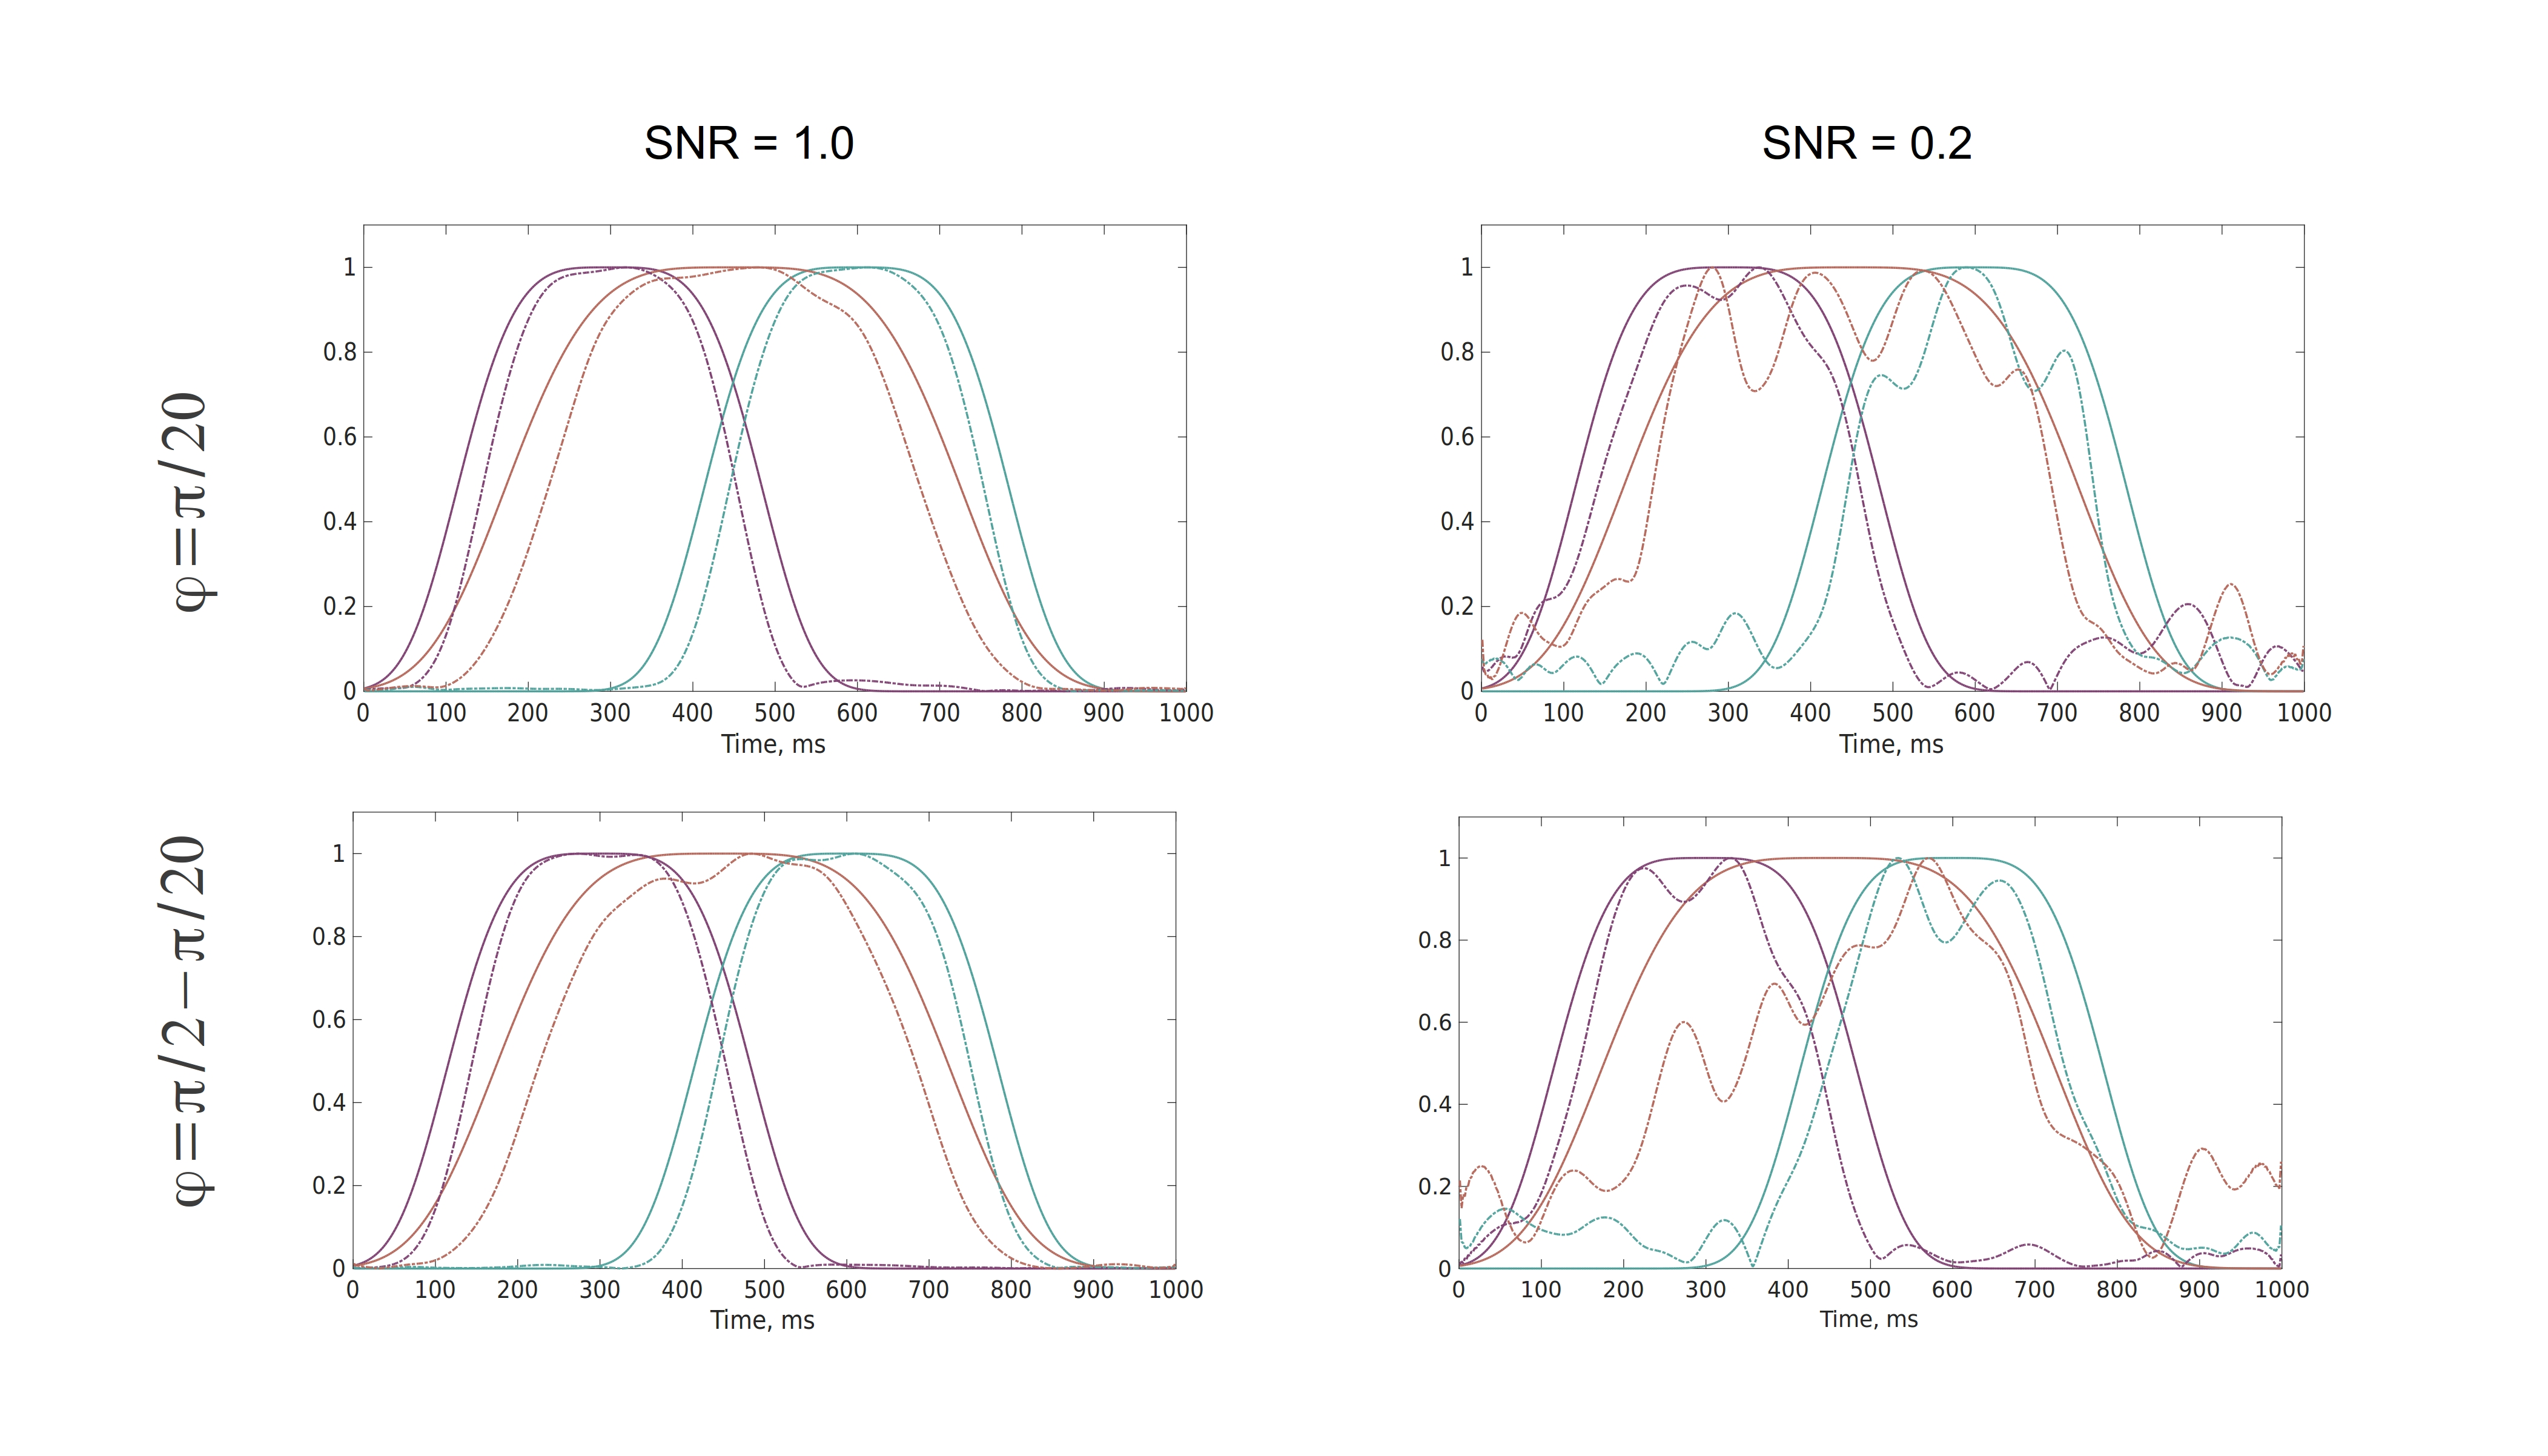
\includegraphics[width=1\textwidth]{../images/psiicos_paper/Figure6_hr.jpg}
    \caption{Временные профили активации симулированных сетей, восстанновленные при помощи PSIICOS, для двух
        значений фазового сдвига и двух значений ОСШ.}\label{fig:06} %Figure 6
        Непрерывные линии отображают истинные симулированные профили, а
        пунктир~--- восстановленные алгоритмом PSIICOS.\@
\end{figure}%

Далее, для системного сравнения четырех рассматриваемых методов на графике~\ref{fig:07}
мы модифицированные кривые Precision-Recall, на которых размером маркера мы отобразили
количество истинных сетей, обнаруженных алгоритмом. На левой части рисунка изображен
полный график Precision-Recall; на панелях (b) и (d) показаны данные в диапазоне 0--0.15.

\begin{figure}[!ht]
 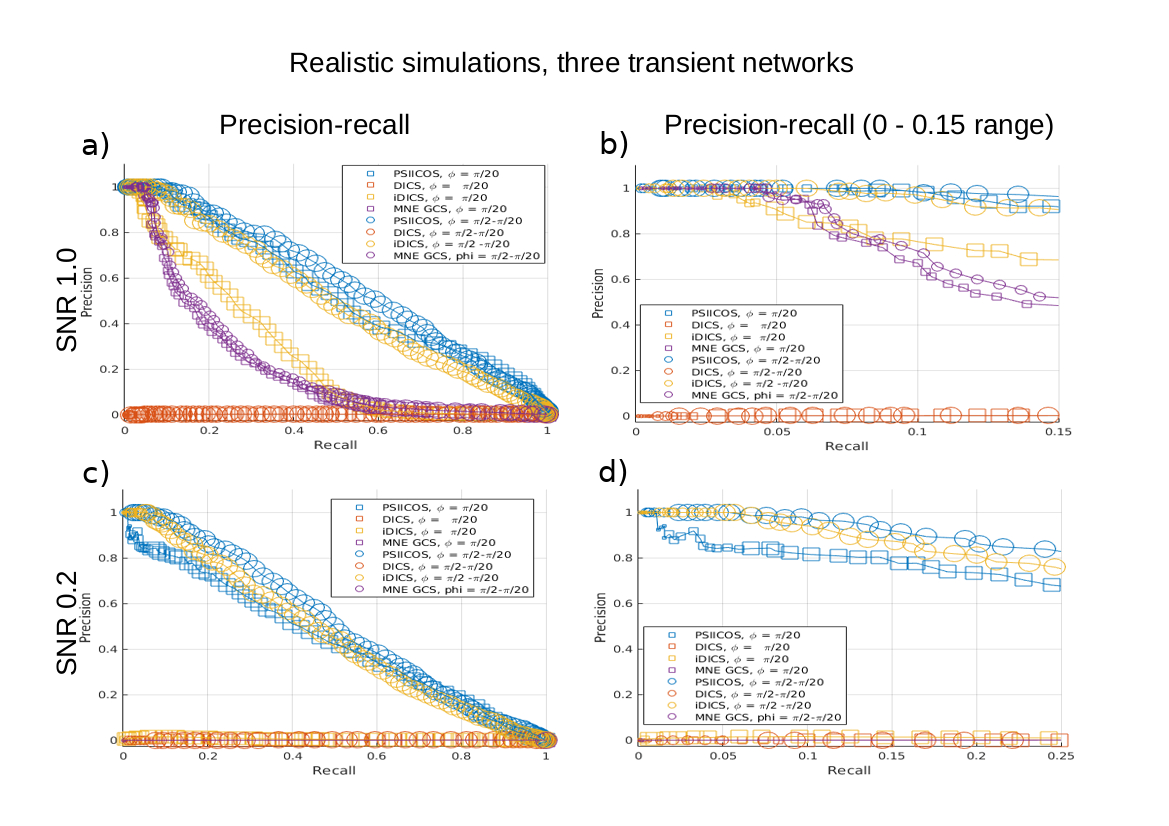
\includegraphics[width=\textwidth]{../images/psiicos_paper/Figure7_hr.jpg}
 \caption{Сравнение PSIICOS с остальными методами в задаче обнаружения трёх
 одновременно активных сетей.}\label{fig:07} %Figure 7
 На рисунках (a), (c) изображены кривые Precision-Recall для всего диапазона
 возможных значений; на рисунках (b), (d) изображены те же кривые, но для
 диапазона значений 0--0.15.
\end{figure}%

Структура этих графиков подтверждает выводы, основанные на визуальном анализе
пространственного распределения обнаруженных сетей (см. рис.~\ref{fig:05}).

Использованные до сих пор метрики оценивают качество решения независимо от порога,
что не годится для оценки качества работы алгоритма на реальных данных.
Для применения к реальным данным мы предлагаем использовать процедуру бутстрэпа,
описанную в разделе~\ref{sec:bootstrap}, чтобы оценить стабильность
получаемых решений и использовать ее в качестве метрики качества.
График~\ref{fig:08} иллюстрирует результаты процедуры
бутстрэпа в применении к реалистичным симуляционным данным.

\begin{figure}[!ht]
 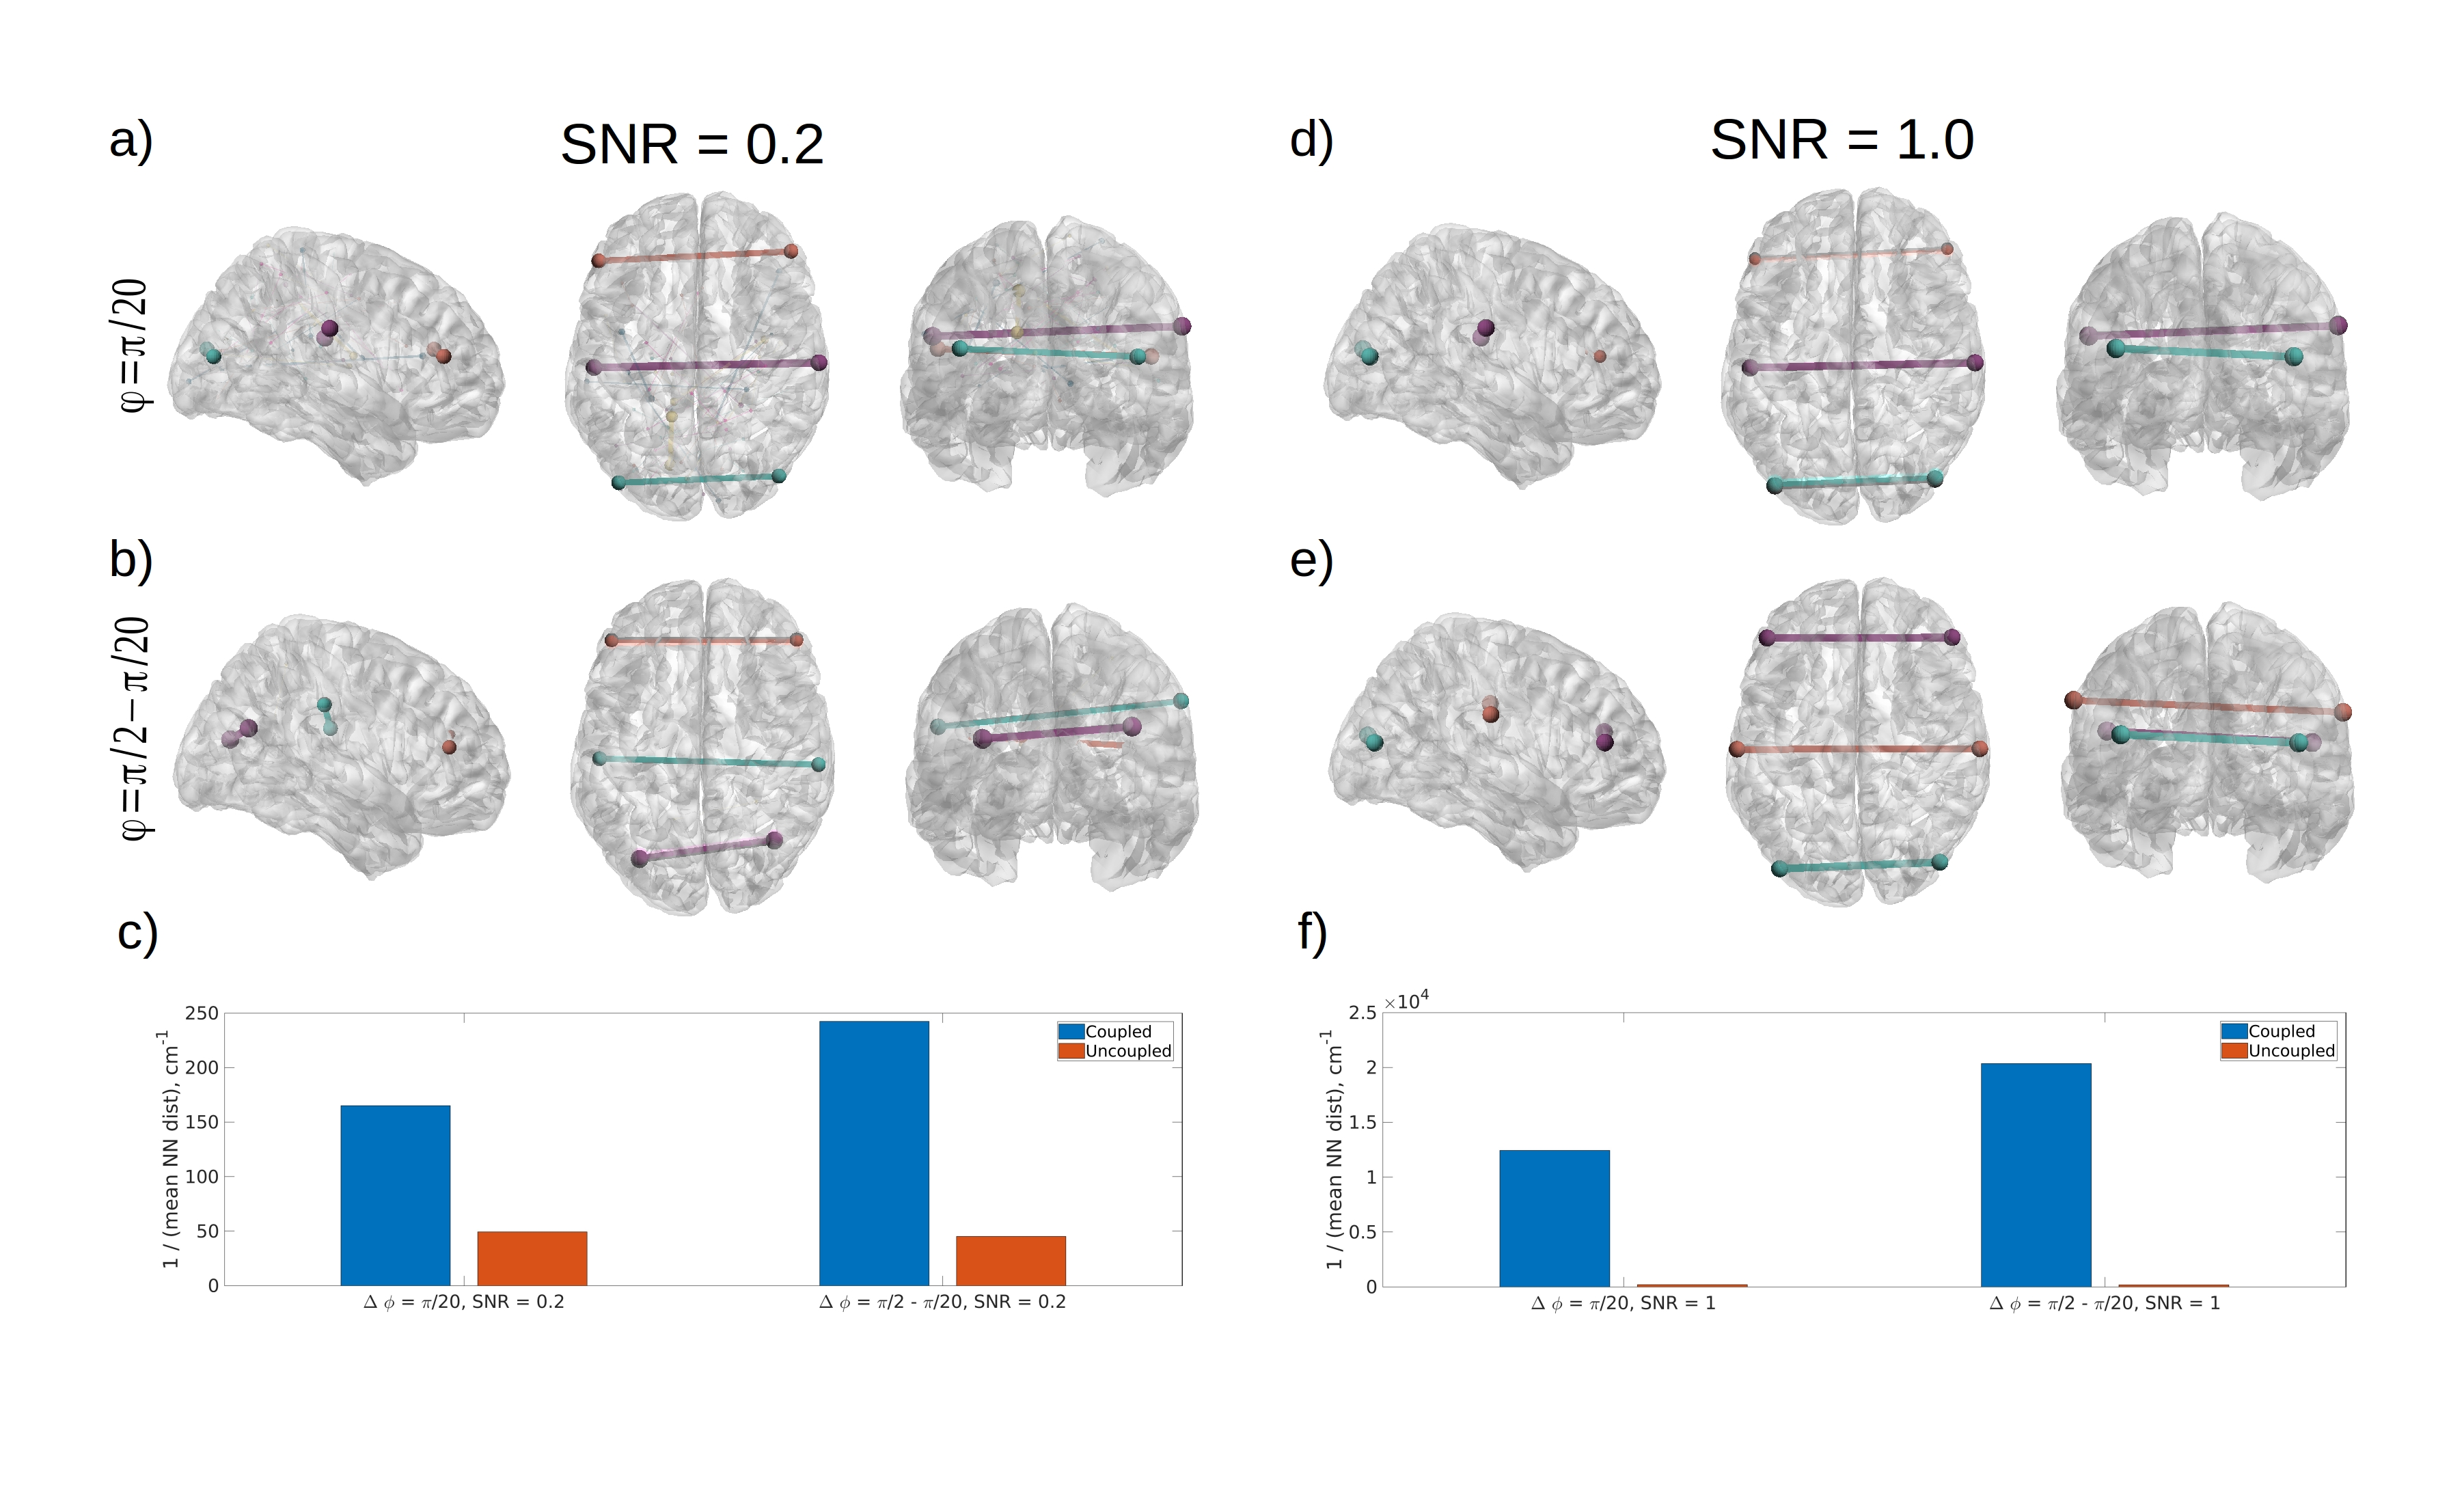
\includegraphics[width=\textwidth]{../images/psiicos_paper/Figure8_hr.jpg}
 \caption{Исследование стабильности метода PSIICOS при помощи процедуры бутстрэпа для
 двух значений фазового сдвига и двух ОСШ.}\label{fig:08}
 (a), (b), (d), (f)~--- стабильные сети отображены в виде отрезков, концы которых
 соответствуют взаимодействующим областям коры. Насыщенность цвета отрезка
 и его концов прямо пропорциональна коэффициенту воспроизводимости $\eta$,
 оцененному при помощи процедуры бутстрэпа. Отрезки, концы которых
 оказывались ближе 1 см друг к другу, мы рисовали одним цветом.
 На графиках (c) и (d) изображен индекс воспроизводимости $\eta$ для
 двух средних фазовых сдвигов, полученных в результате описанной процедуры
 бутстрэпа для двух различных значений ОСШ (ОСШ=0.2 и ОСШ=1 соответственно).
\end{figure}% Figure 8


Наши симуляции показывают, что предложенный подход позволяет достичь лучшего
качества решений при поиске взаимодействующих источников как при околонулевых,
так и при близких к $\pi/2$ фазовых сдвигах. Более того, алгоритм PSIICOS
позволяет обнаруживать сети для всего спектра возможных фазовых задержек. Чтобы
дополнительно проиллюстровать это качество, мы применили предложенный метод к
симуляционным данным с тремя сетями на равномерной сетке фазовых задержек в
диапазоне от 0 до $\pi/2$. Этот анализ мы провели для двух значений ОСШ и
сравнили три различных подхода: использование только мнимой части (iDICS),
использование только спроецированной действительной части и использование
полной кросс-спектральной матрицы (PSIICOS). На графике~\ref{fig:09}
изображена метрика качества решения в каждом из случаев для различных фазовых
сдвигов.  В качестве метрики мы использовали площадь под кривой
Precision-Recall. Для значений фазы, близких к $\pi/2$, информация о взаимодействующих
источниках содержится в основном во мнимой части кросс-спектра, что легко
заметить из графика~\ref{fig:09}, где использование только мнимой части позволяет достичь
высокого качества решения для близких к $\pi/2$ фазовых сдвигов. Для реалистичного
значения ОСШ=0.1 качество решения резко ухудшается как только значение фазового сдвига
покидает окрестность точки $\pi/2$.

\begin{figure}[!ht]
 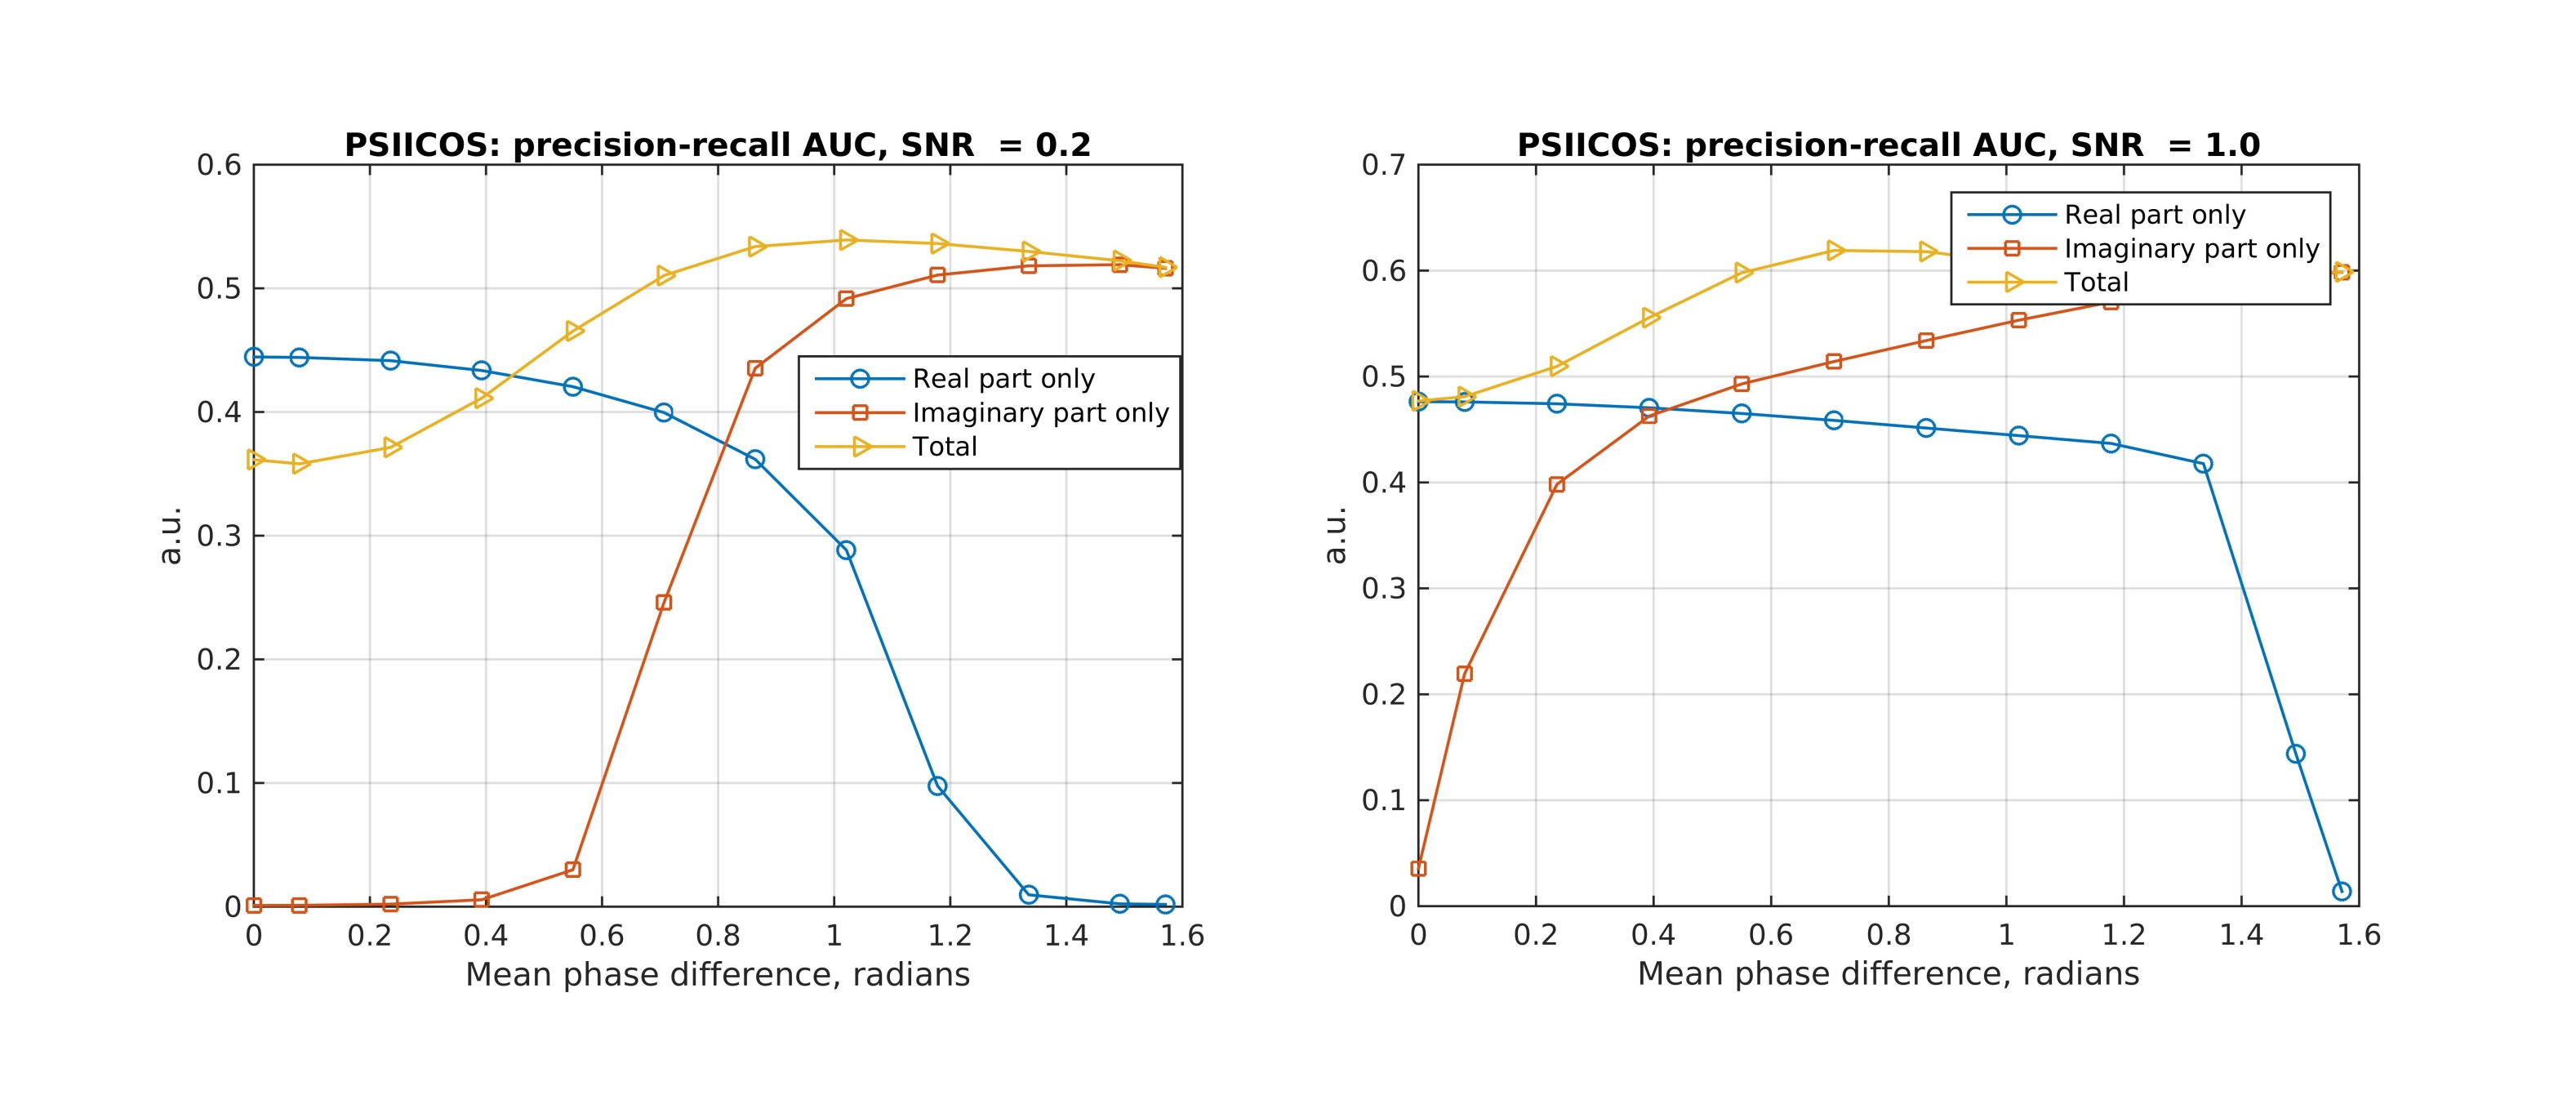
\includegraphics[width=1\textwidth]{../images/psiicos_paper/Figure9_hr.jpg}
 \caption{Качество решений алгоритма PSIICOS как функция средней фазовой задержки}\label{fig:09}
     (a)~--- для низкого значения ОСШ и (b)~--- для высокого.
     Для близких к $\pi/2$ средних значений фазового сдвига информация
     о взаимодействии источников содержится в основном во мнимой части кросс-спектра.
     Поэтому использование только мнимой части (что эквивалентно iDICS) позволяет
     достигать высокого качества решения; качество решения при этом затухает
     с уменьшением фазового сдвига. С другой стороны, для близких к нулю
     значений фазовой задержки информация о взаимодействии содержится в основном
     в действительной части кросс-спектра. Действительная часть загрязнена
     протечкой сигнала, которая может быть удалена при помощи PSIICOS-проекции.
     После этого очищенная действительная часть используется для обнаружения
     сетей с близкими к нулю фазовыми задержками (синие кривые). Одновременное
     использование действительной и мнимой компоненты позволяет добиться равномерного
     качества решений по всему диапазону средних фазовых сдвигов (оранжевая кривая).
\end{figure}% Figure 9

С другой стороны, для близких к нулю сдвигов информация о коннективности содержится
в основном в действительной части. Действительная часть загрязнена протечкой сигнала, которую
мы эффективно удаляем PSIICOS-проекцией. Далее спроецированная действительная часть
может быть использована для обнаружения сетей с близкими к нулю значениями фазового
сдвига. Предложенный метод PSIICOS позволяет использовать очищенную действительную
и мнимую части совместно для достижения равномерного по фазовым сдвигам качества решения.

\section{Сравнение на реальных данных.}\label{sec:validation_on_real_data}
Так как главной целью данного
исследования является изложение новой методологической базы для оценки
коннективности и валидации результатов при помощи симуляций, важно
проиллюстрировать поведение метода на МЭГ данных из реального эксперимента.
Тем не менее, полный групповой анализ и систематическое сравнение с другими
методами лежит за пределами этого в большей степени методологического исследования.
Поэтому нашей задачей было продемонстрировать, как наш метод может быть использован на
реальных данных и оценить его устойчивость.
Необходимо понимать, что оценка работы метода на
реальных данных не способна предоставить критерий качества работы алгоритма, так как
мы не знаем истинной картины взаимодействия участков коры. В то же время мы можем
продемонстрировать методику возможного использования нашего алгоритма и оценить
его усточивость к изменчивой структуре данных методом бутстрэпа.

Мы применили предложенный метод для анализа реальных МЭГ-данных, полученных для
исследования воображаемых вращений в статье~\cite{DeLange2008}. Часть данных
для одного испытуемого была выложена в свободный доступ в ходе соревнования по
анализу данных на конференции Biomag 2010.

В эксперименте испытуемый определял латеральность изображенной на экране кисти
руки нажатием на одну из двух соответствующих кнопок.  Изображения рук были
повернуты к наблюдателю на некторый угол, и для ответа испытуемый должен был
мысленно их повернуть. Авторы статьи исследовали электрическую активность коры
при осуществлении воображаемых вращений.

Данные содержали 800 эпох с рандомизированными углами поворота и
латеральностями. Эти 800 эпох были разделены на 5 блоков. Каждая эпоха включала
следующую последовательность событий: фиксационный крест (3 сек. предъявления),
изображение руки (предъявление до момента ответа испытуемого), фиксационный
крест (0.5 сек.), окрашенный в красный или зеленый цвет в зависимости от
правильности ответа испытуемого. В среднем испытуемые проводили в МЭГ-сканнере
70 минут.

В ходе эксперимента мозговая активность регистрировалась МЭГ-устройством
системы VSM/CTF Systems, включающим 151 аксиальный градиометр. Аналоговый
сигнал был отфильтрован  фильтром нижних частот с частотой среза 300 Гц и
сэмплирован на частоте 1200 Гц. После удаления артефактных сегментов для
анализа осталось 259 эпох, соответствующих изображениям левой руки. Их
длительность лежала в пределах от 1.52 сек до 2.08 сек. Мы выровняли эпохи
таким образом, чтобы начало каждой эпохи соответствовало моменту 0.5 сек до
предъявления изображения. Для анализа мы брали 1 секунду после предъявления
стимула.

Для анализа мы использовали следующие полосы частот: тета (4--8 Гц), альфа
(8--12 Гц), бета (16--24 Гц), нижняя гамма (30--60 Гц), верхняя гамма (65--85
Гц).

На первом шаге мы применяли полосовой КИХ-фильтр с нулевой фазой для отделения
целевой полосы частот. Далее мы усредняли по эпохам внешние произведения
временных рядов с примененным преобразованием в аналитический сигнал. Таким
образом мы получали временной ряд кросс-спектра в виде трехмерного массива,
который после векторизации задавался матрицей $M^2 \times T$, где $M=151$~---
количество сенсоров в установке. Далее мы применяли к временному ряду
кросс-спектра PSIICOS-проекцию с рангом $R=150$, который мы определяли исходя
из соображений, изложенных в разделе~\ref{sec:subspaces_attenuation}. Мы
проводили анализ и с другими значениями параметра $R$ в диапазоне от 100 до
250, и в этих пределах ранг проекции не оказывал значительного влияния на
решение.

Далее мы отдельно анализировали действительную и мнимую части векторизованного
временного ряда кросс-спектра. Вместо простого усреднения вдоль временной оси
для восстановления пространственной структуры мы вычисляли SVD-разложение
действительной и мнимой части спроецированного кросс-спектрального временного
ряда. Далее мы проводили поиск сетей-источников для первых двух левых
собственных векторов мнимой и действительной части на подробной сетке из 15000
узлов.

Для проверки стабильности получаемых решений мы использовали процедуру
бутстрэпа, описанную в разделе~\ref{sec:bootstrap} для $m=30$ и $B=100$ и
отрисовывали индекс воспроизводимости $\eta$.  Мы отображали полученные сети
только в рамках стабильных, воспроизводимых на бутстрэпе пучков сетей. Сети,
которые отстояли друг от друга на расстояние меньше 1см, мы рисовали одним
цветом.  Также для каждой воспроизводимой компоненты мы рисовали временной
профиль активации как правый собственный вектор временного ряда кросс-спектра.

% \section{Результаты.}\label{results}



На графике~\ref{fig:10} мы отобразили результаты частотно-специфичного
анализа воспроизводимости решения. На графике изображена величина, обратная к
расстоянию до ближайшей сети, сгруппированая по 5 полосам частот для
действительной и мнимой частей. Как видно из графика, сети, обнаруженные с
использованием действительной части кросс-спектра, оказываются более
воспроизводимыми, чем сети, обнаруженные по мнимой части. Наиболее воспроизводимые
сети по действительной части, находятся в бета и обоих гамма-диапазонах.
Воспроизводимые сети по мнимой части кросс-спектра принадлежат полосам частот
альфа, бета и верхняя гамма. Важно отметить, что хотя сети по действительной части
в целом характеризуются большей воспроизводимостью, это оказывается не так для
полосы частот альфа.

\begin{figure}[h!tpb]
 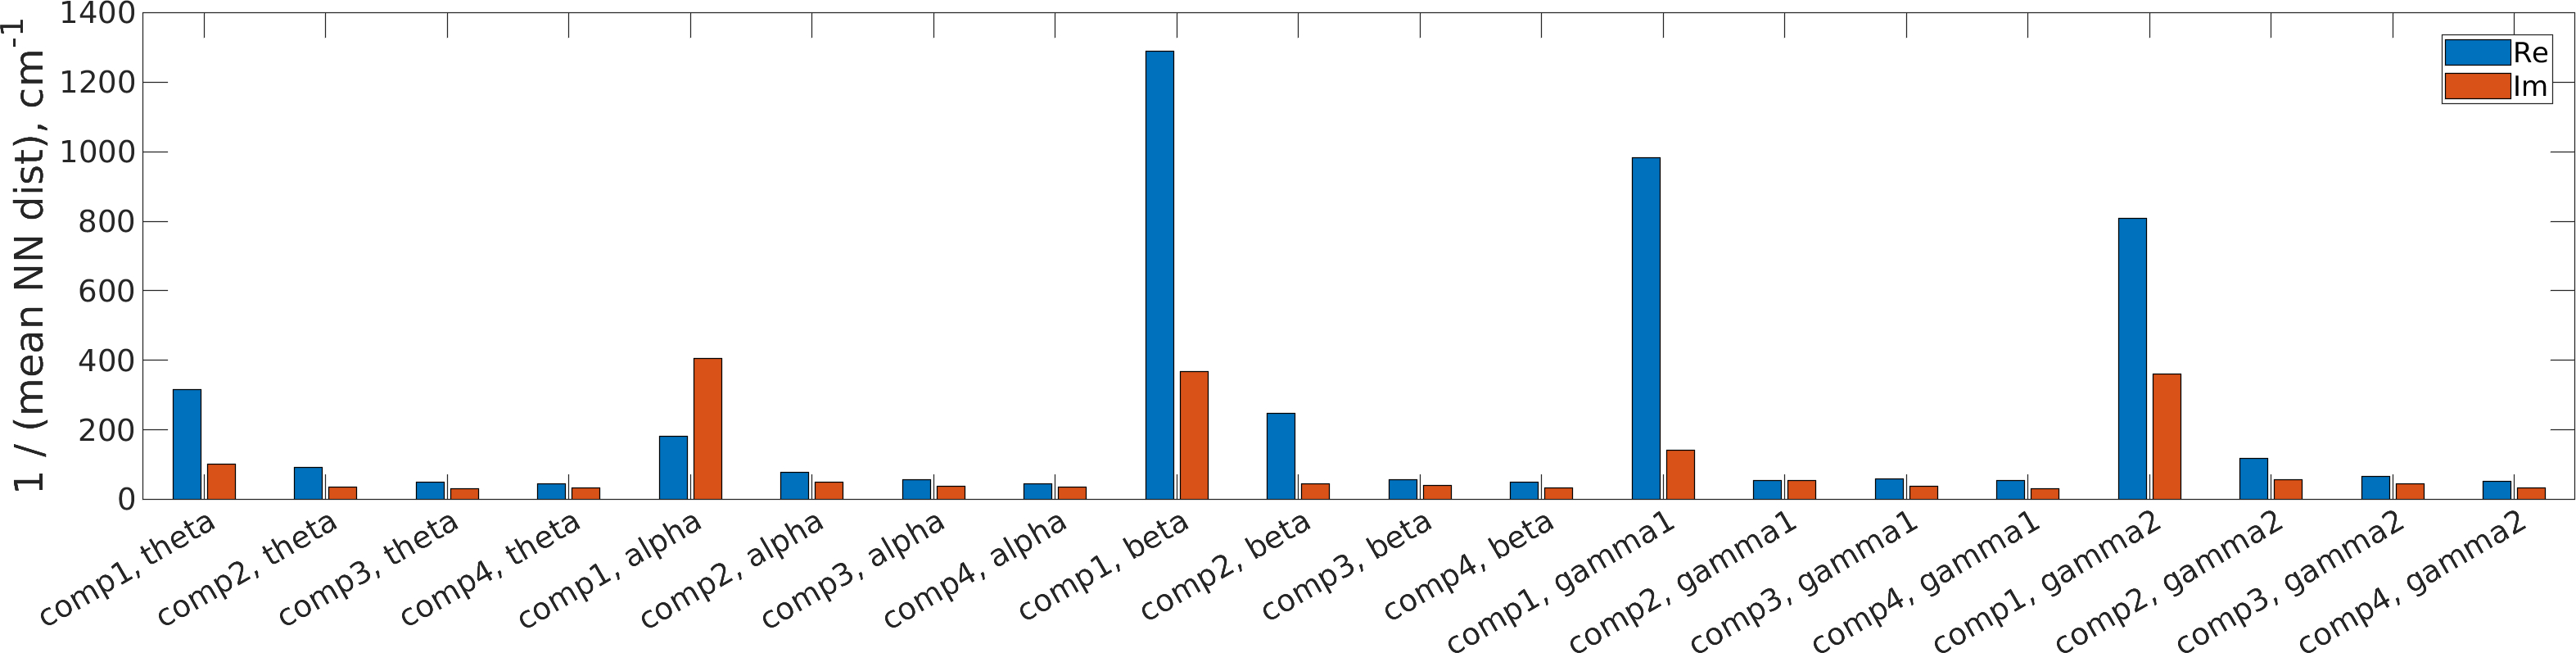
\includegraphics[width=1\textwidth]{../images/psiicos_paper/Figure10_hr.jpg}
 \caption{Полосы частот с наиболее воспроизводимыми сетями, определенными при помощи
 процедуры бутстрэпа.}\label{fig:10}
 Бутстрэп проводился последовательным выбором подмножества эпох, на котором
 вычислялся кросс-спектр, к которому затем применялась PSIICOS-проекция.
 Столбики на графике отображают индекс воспроизводимости, который вычислялся
 как обратное к среднему расстоянию до ближайшего соседа для каждой отдельной
 сети, найденной по мнимой и действительной спроецированной части кросс-спектра для четырех
 наиболее значимых главных компонент. Результаты для действительной части представлены
 синим цветом, а для мнимой~--- желтым.
 \end{figure} %Figure 10

 На графиках~\ref{fig:11},~\ref{fig:12},~\ref{fig:13} изображена пространственная
структура обнаруженных сетей для этих частотных диапазонов. Сети, узлы которых
оказывались ближе 1 сантиметра друг к другу, мы рисовали одним цветом. Перекрывающиеся сети
мы рисовали с увеличинным размером маркера и увеличенной толщиной линии. Прозрачность
линии мы меняли в зависимости от плотности сетей в кластере с учетом перекрытий.
Также для каждой воспроизводимой компоненты мы рисовали профиль ее временной активации
как правый собственный вектор сингулярного разложения соответствующей части временного
ряда кросс-спектра.

\begin{figure}
\centering
\text{Тета- (3--6 Гц) и альфа- (8--12 Гц) диапазоны}

 \begin{subfigure}[b]{0.4\textwidth}
 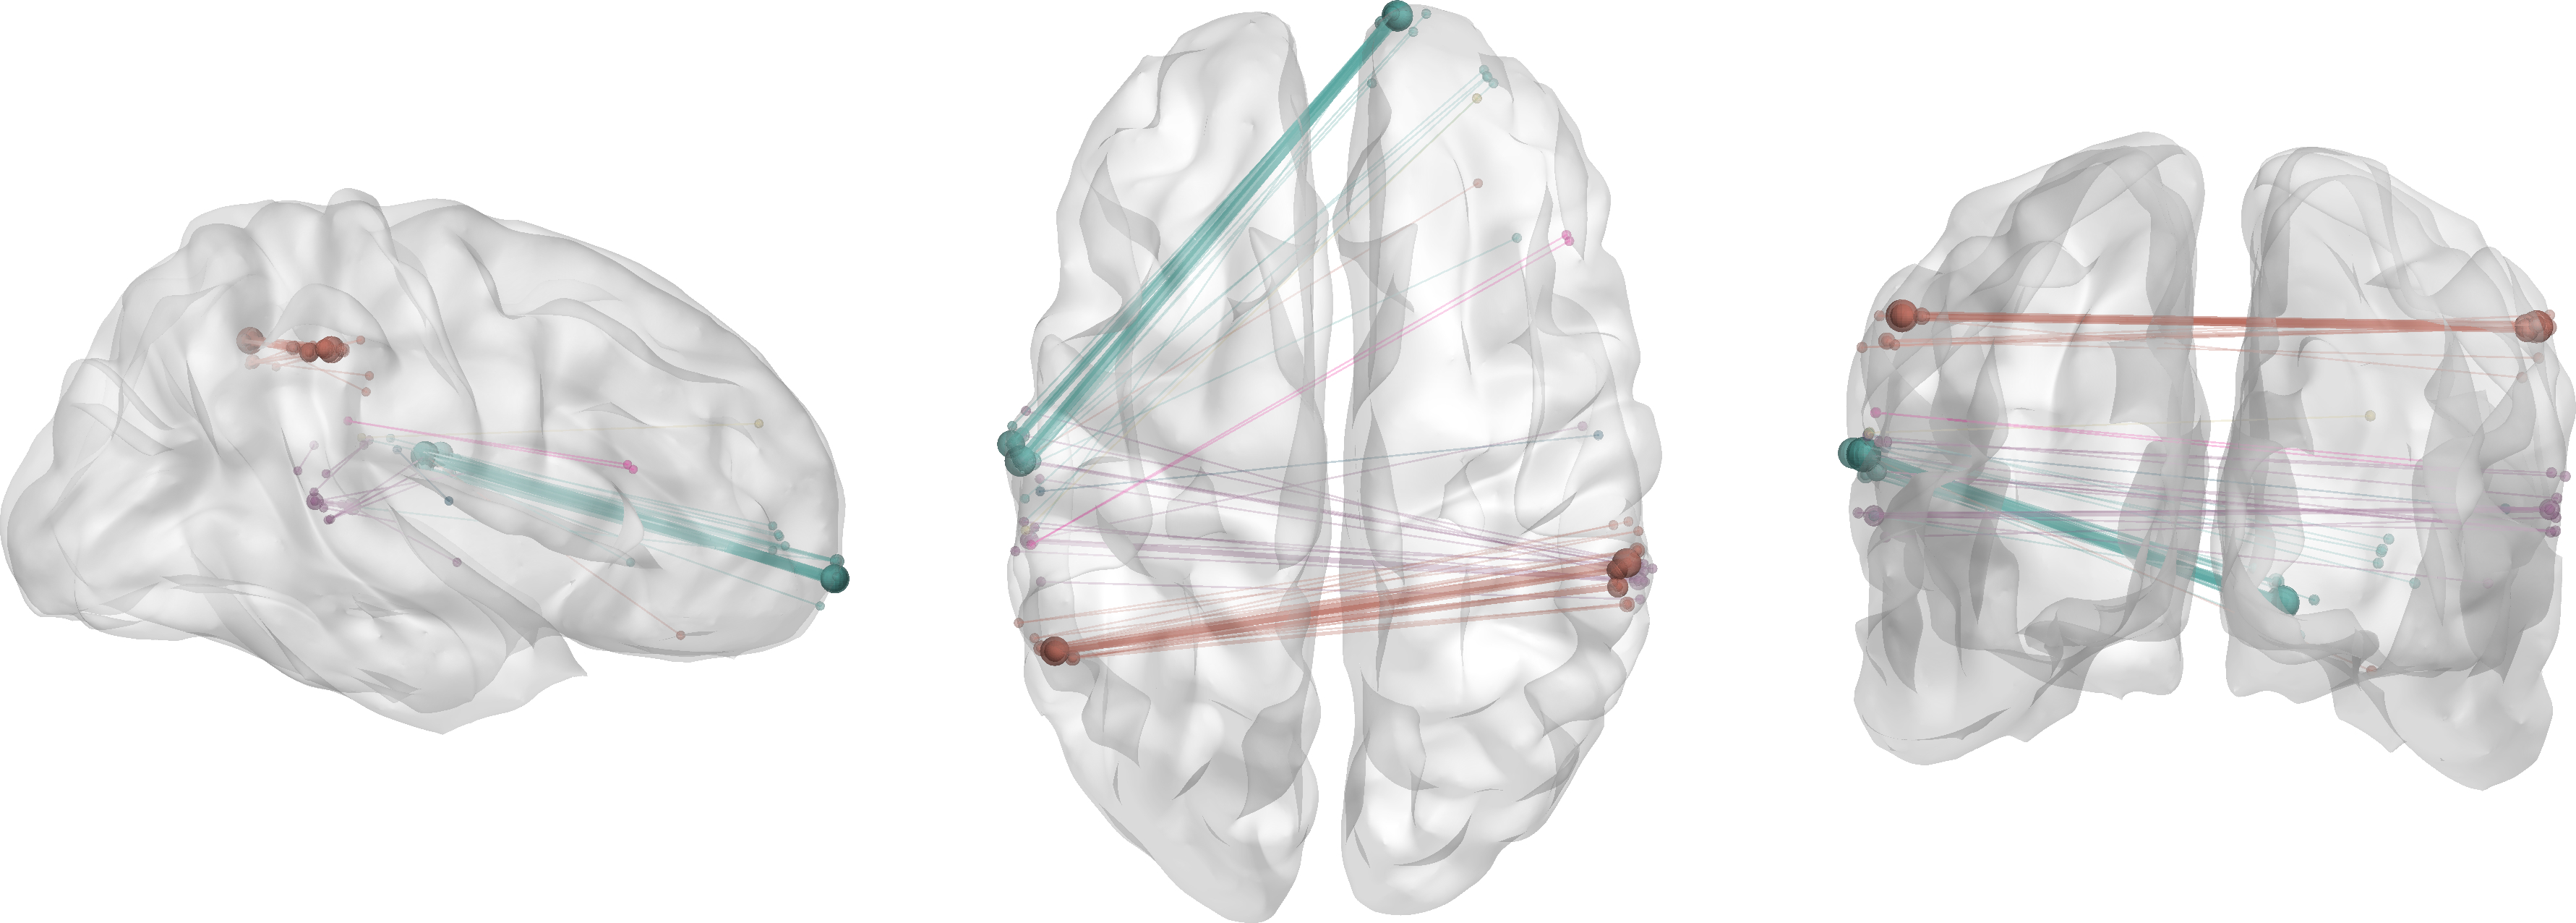
\includegraphics[width=\textwidth]{../images/psiicos_paper/Figure11_a1.jpg}
 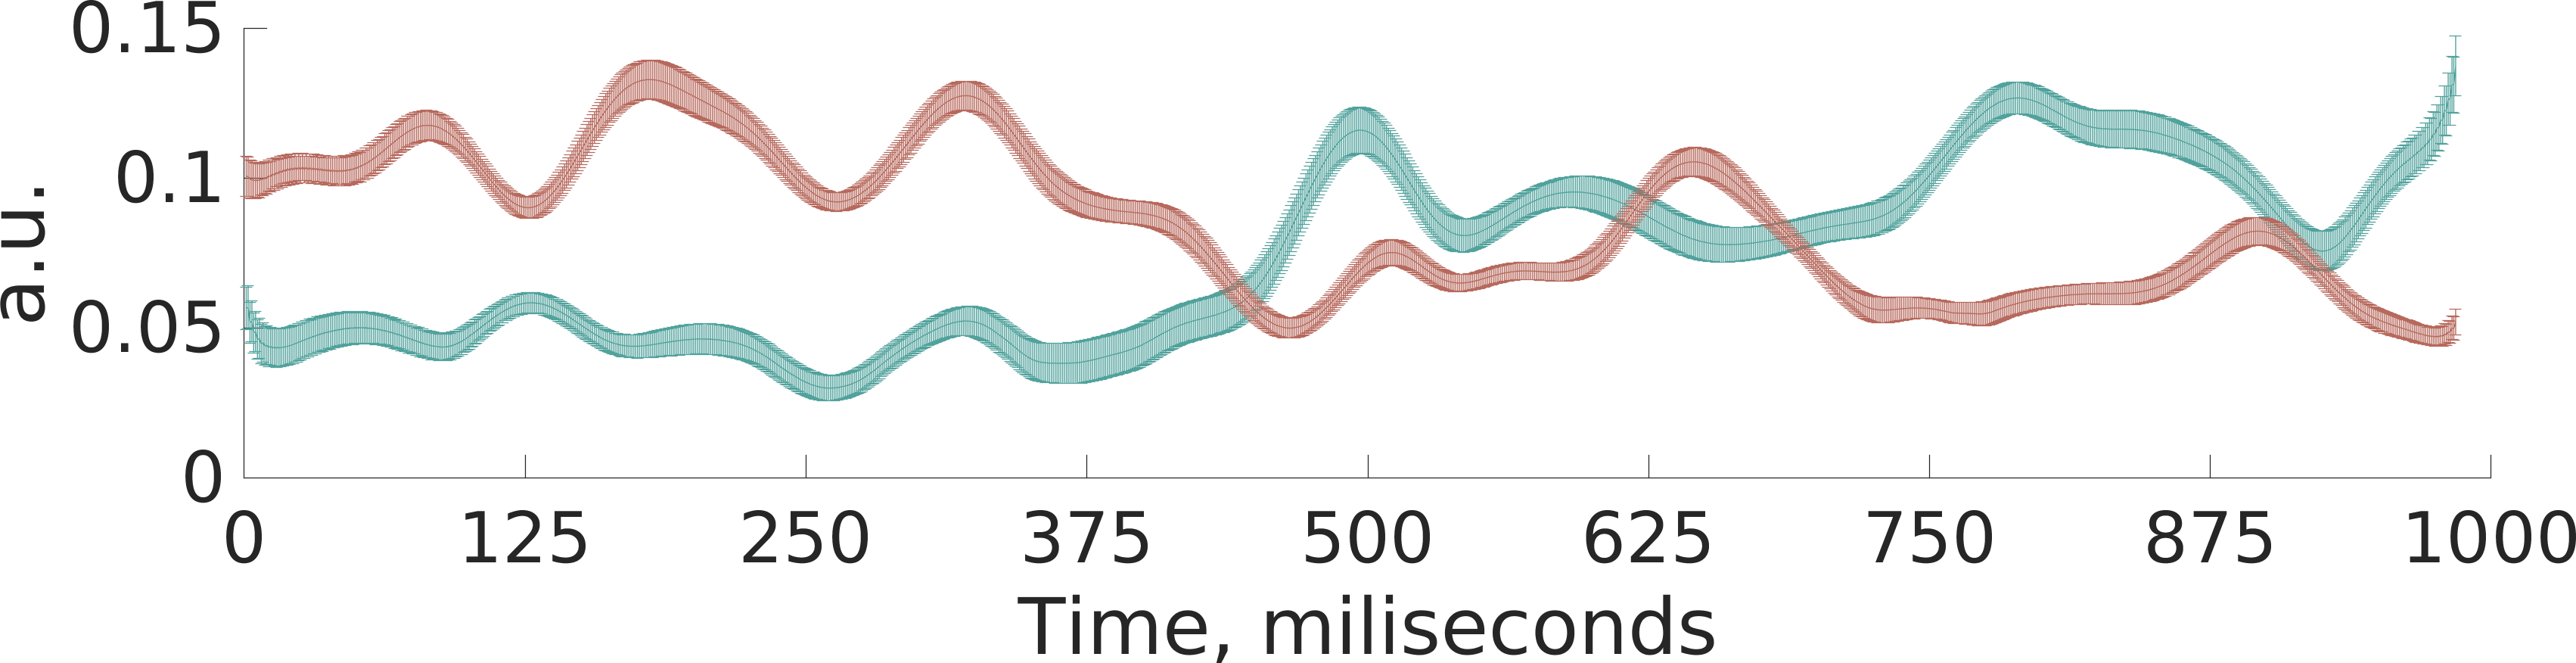
\includegraphics[width=\textwidth]{../images/psiicos_paper/Figure11_a2.jpg}
 \caption{Тета-диапазон, Re, сеть 1}\label{fig:11a}
 \end{subfigure}
 \hspace{1cm}
 \begin{subfigure}[b]{0.4\textwidth}
 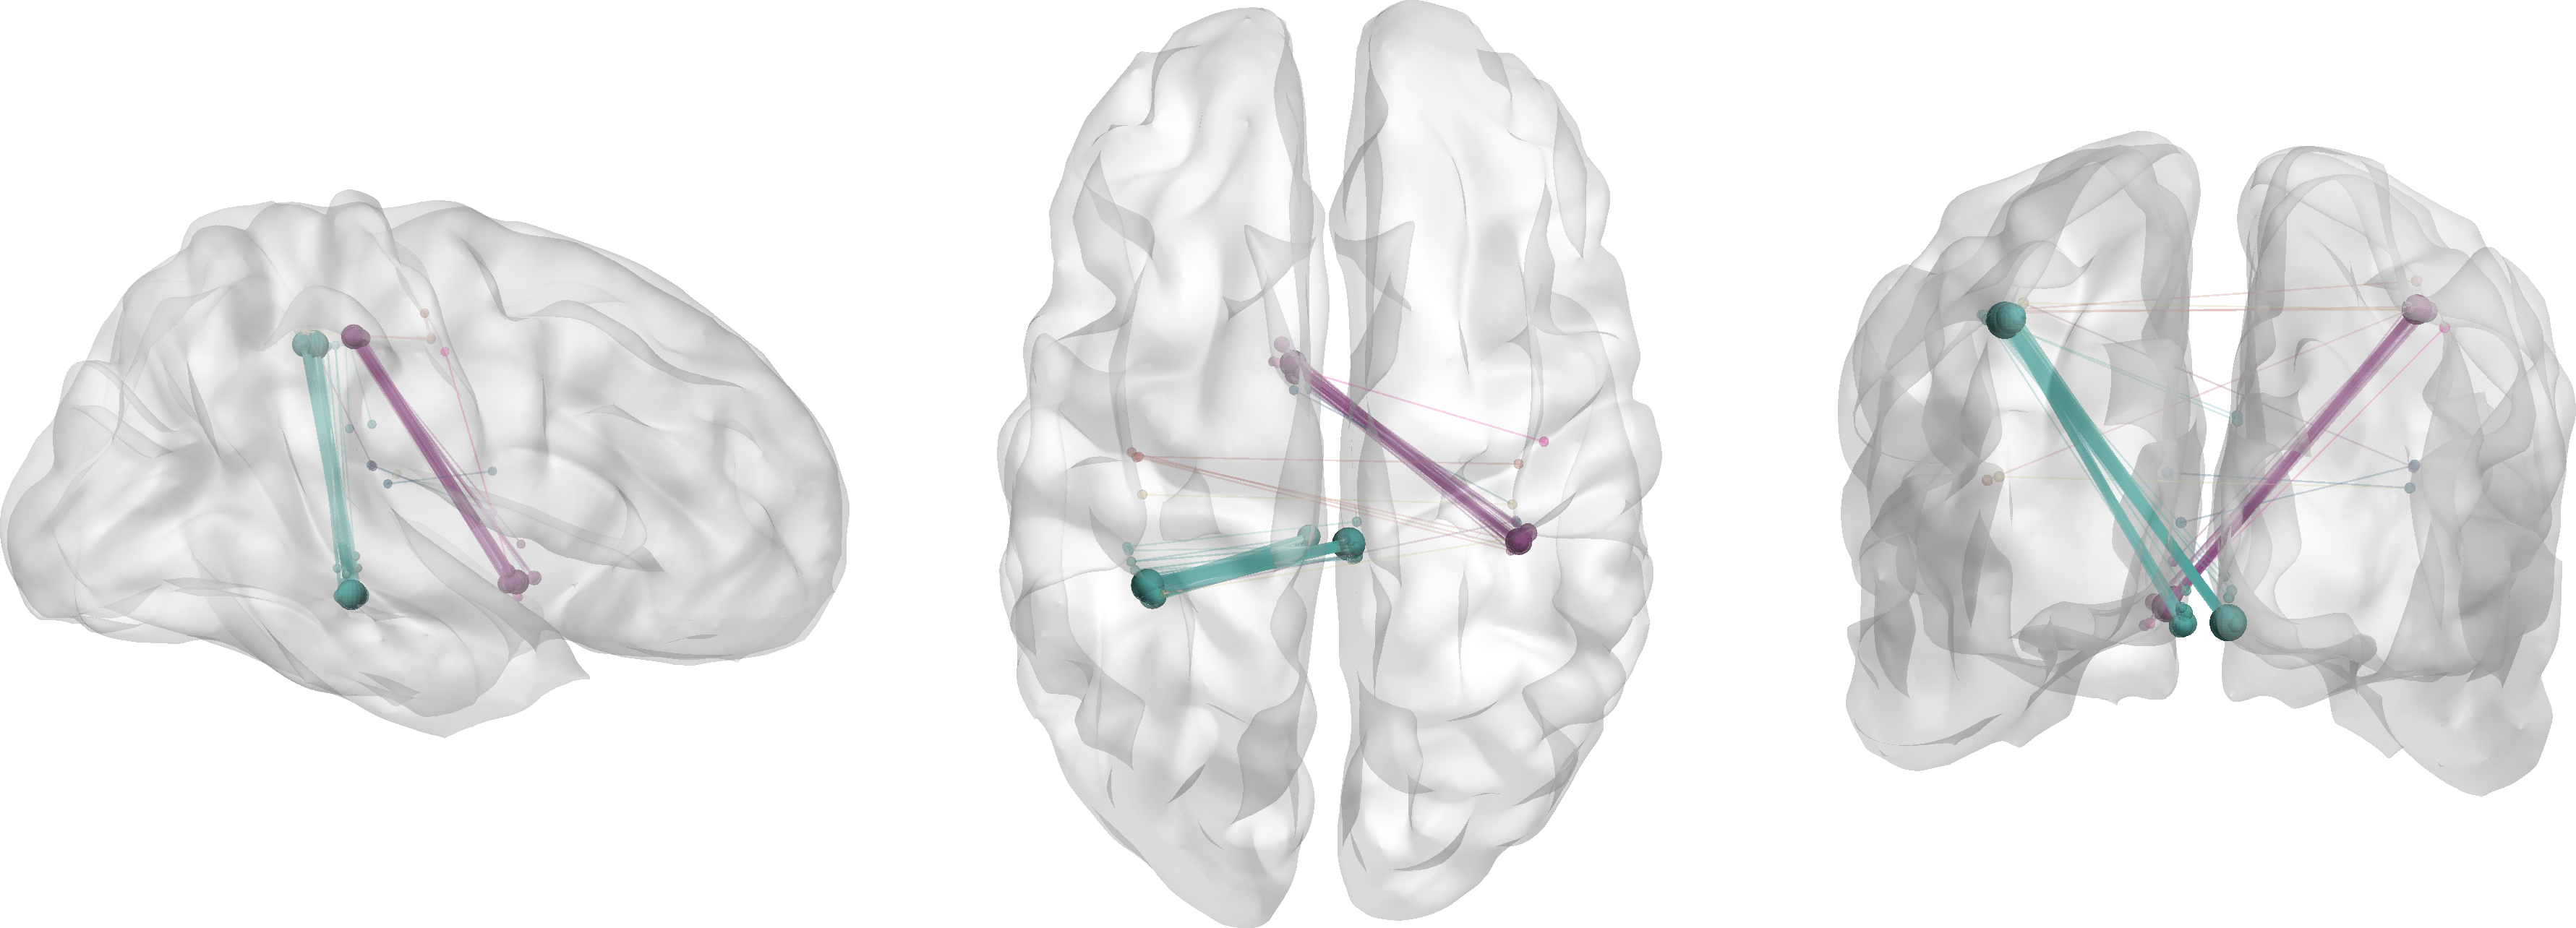
\includegraphics[width=\textwidth]{../images/psiicos_paper/Figure11_b1.jpg}
 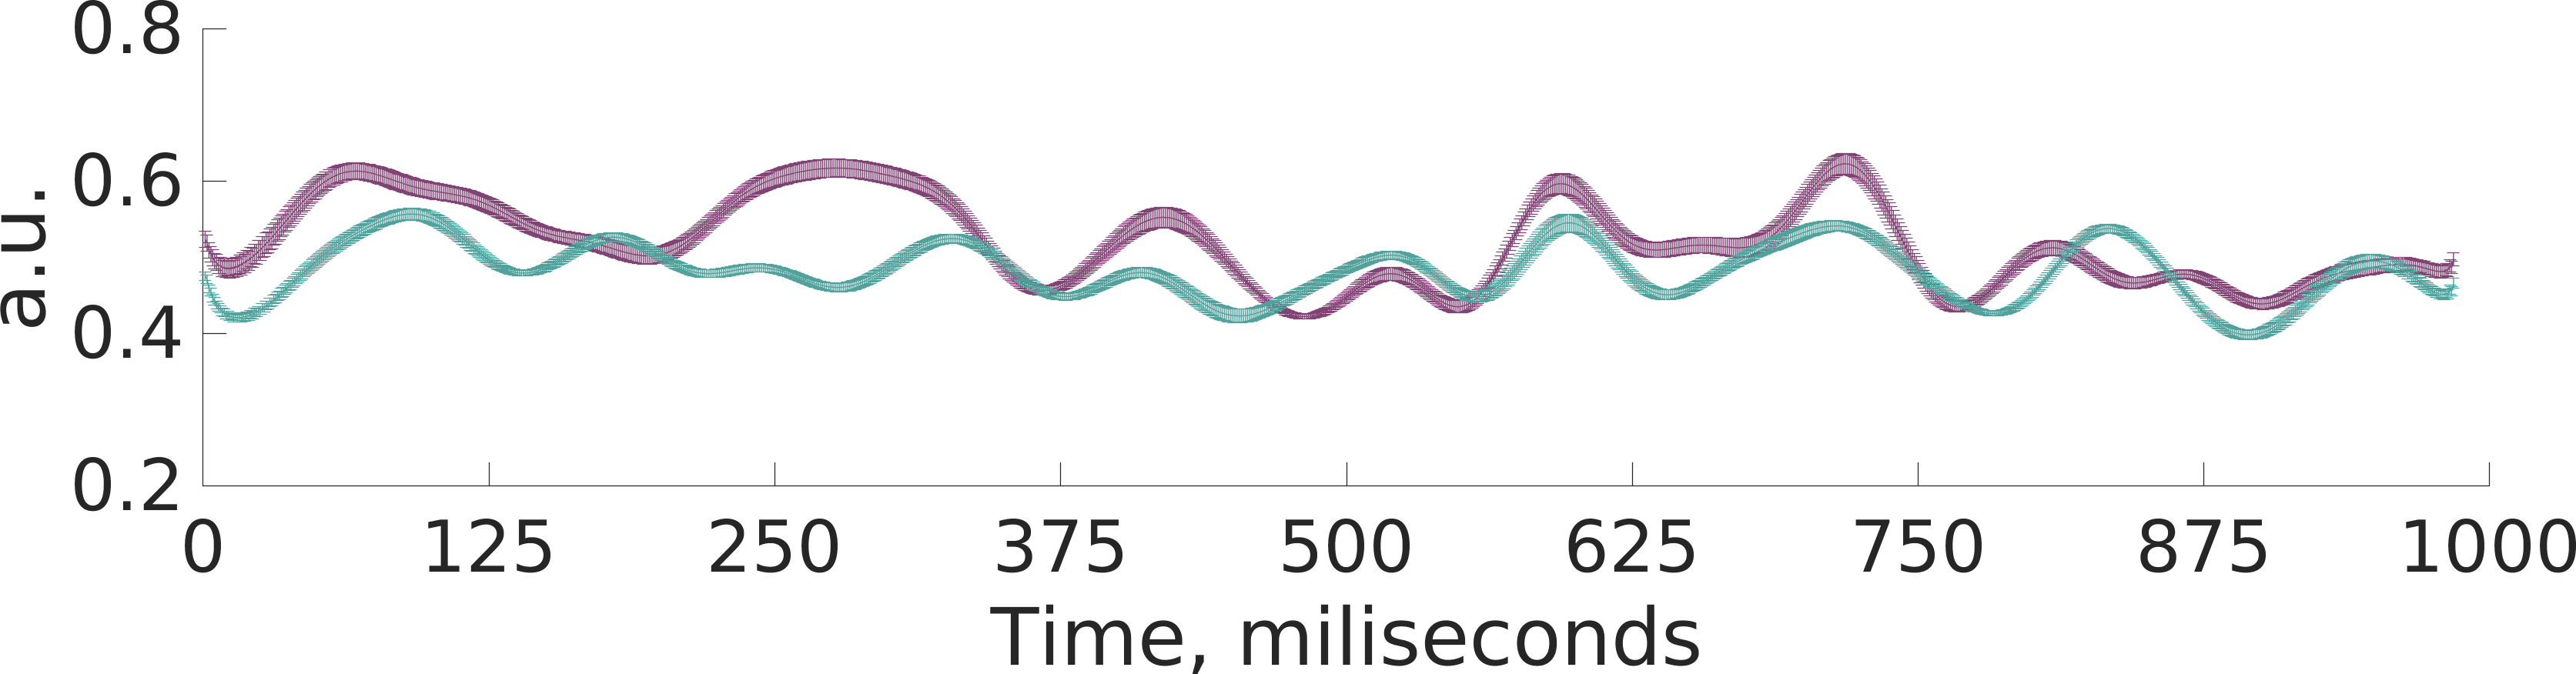
\includegraphics[width=\textwidth]{../images/psiicos_paper/Figure11_b2.jpg}
 \caption{Альфа-диапазон, Im, сеть 1}\label{fig:11b}
 \end{subfigure}
 \caption{Пространственная структура и временная динамика наиболее воспроизводимых сетей в диапазонах частот тета (3--6 Гц) и альфа (8--12 Гц)}\label{fig:11}
\end{figure} % figure 11

Анализ действительной части кросс-спектра показывает наличие следующих сетей с преимущественно
малыми фазовыми задержками. В тета-диапазоне (рис.~\ref{fig:11}) мы видим сети,
соединяющие правую орбито-фронтальную кору, вовлеченную в сенсорную интеграцию, с левым
билатеральным височно-теменным узлом, про который известно, что он активен при воображении
движения~(\cite{Hanakawa2008}). Также мы видим кросс-латеральную сеть, соединяющую два
теменных отдела.

В бета-диапазоне мы видим механистически правдоподобную кросс-латеральную связь
между вентральным зрительным путем и зоной репрезентации руки в моторной
области правого полушария. Дополнительно мы наблюдаем взаимодействие между
зонами представительства руки сенсомоторной области правого полушария и
соматосенсорной области левого, рис.~\ref{fig:12}, что частично
согласуется с наблюдениями, описанными в статье~\cite{Lamm2007} и соотносится
с профилями функциональной коннективности, описанными в  фМРТ-исследовании
воображаемых вращений~\cite{Striem-Amit2017}. Наконец, мы обнаружили взаимодействие
зоны представительства руки в моторной области правого полушария с височным полюсом
левого полушария в гамма-диапазоне, рис.~\ref{fig:13a}, а также с
орбито-фронтальной зоной левого полушария в верхнем гамма-диапазоне, рис.~\ref{fig:13b}.
Правдоподобность этих наблюдений подкреплена предполагаемой
ролью височного полюса левого полушария, в которую входит ``\ldots визуальное различение
двумерных изображений и мнемоническая функция соотнесения и научения'' (\cite{Dupont2002}).

\begin{figure}
\centering
\text{Бета-диапазон (16--24 Гц)}

 \begin{subfigure}[b]{0.4\textwidth}
 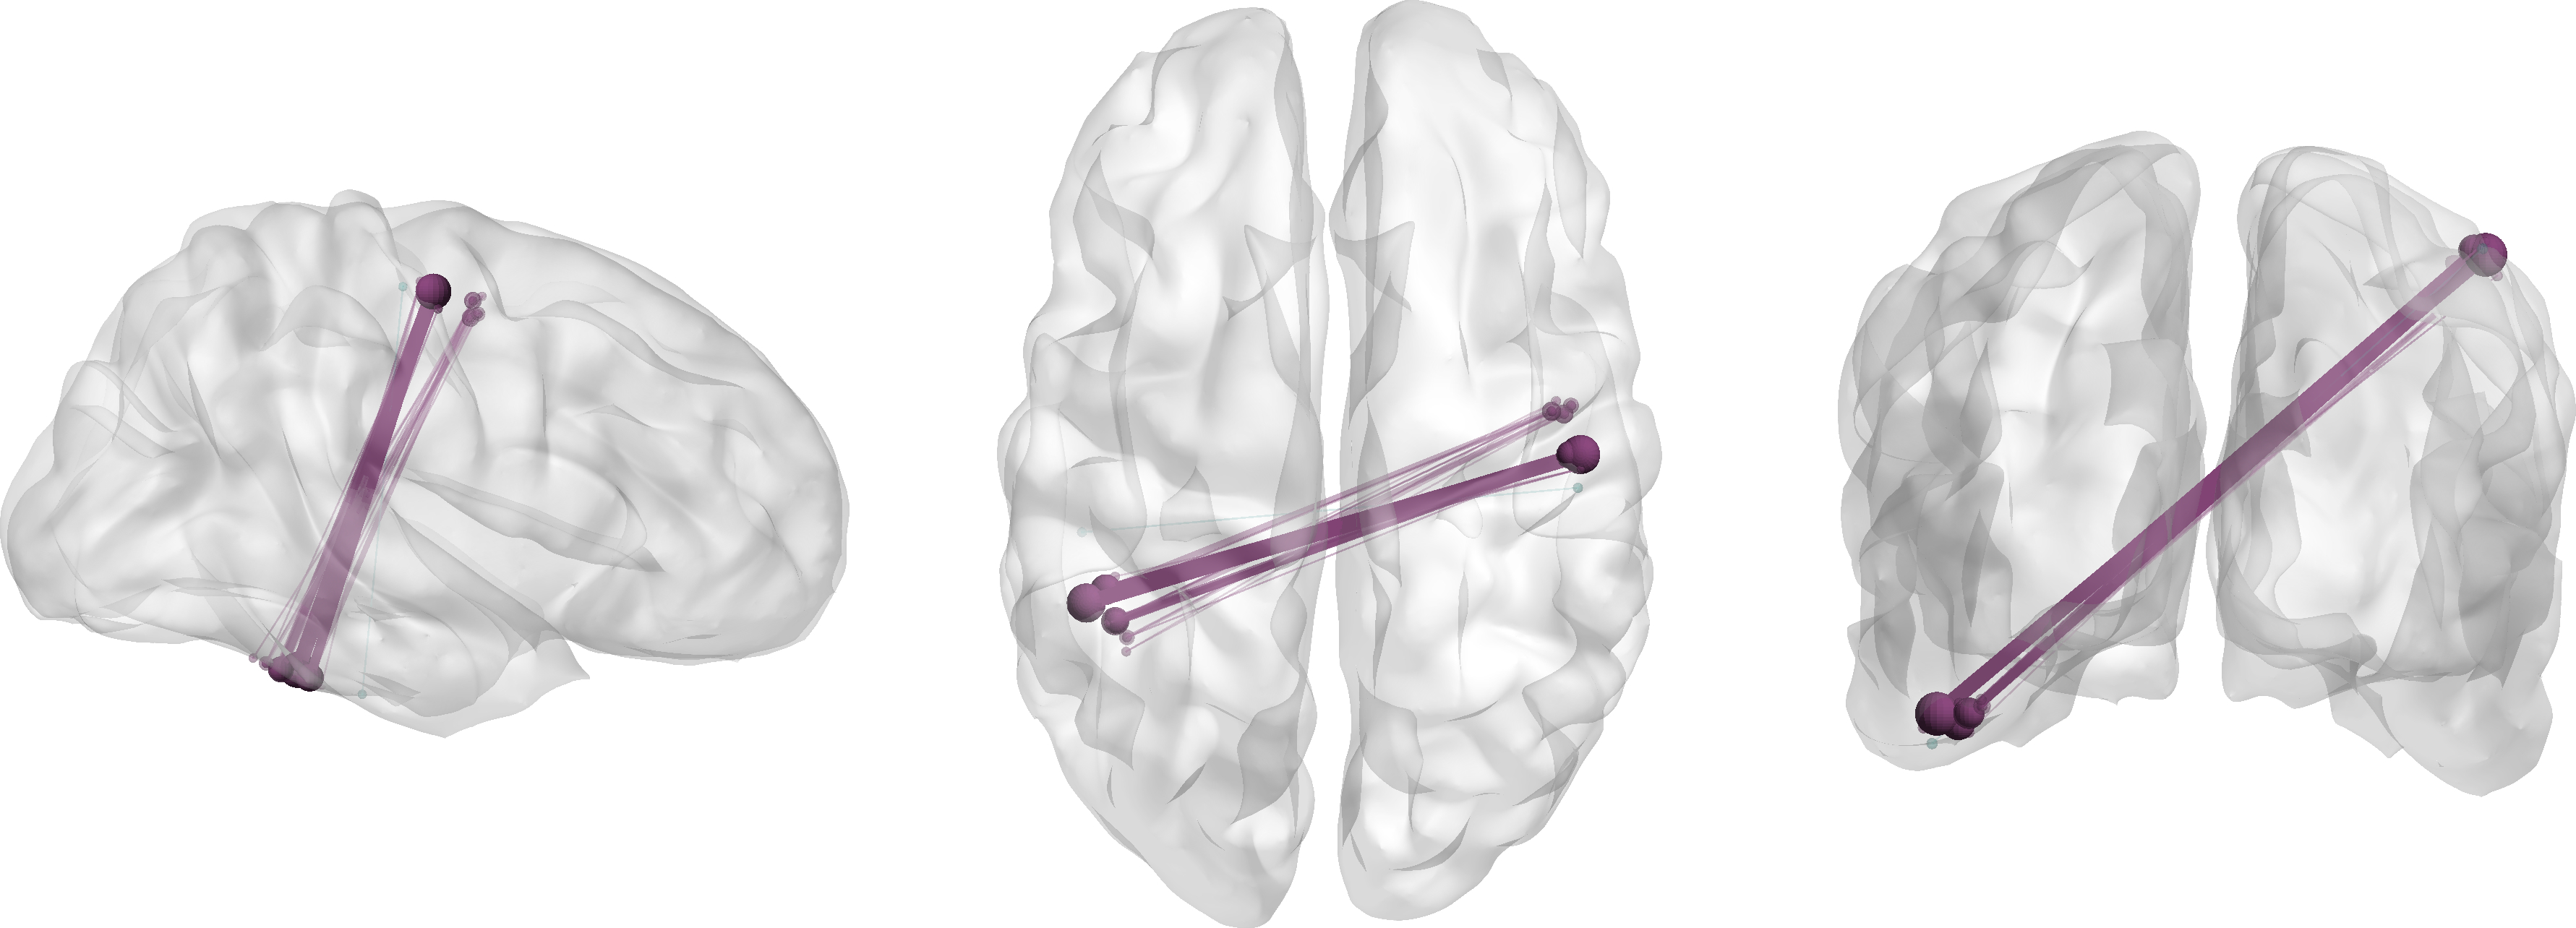
\includegraphics[width=\textwidth]{../images/psiicos_paper/Figure12_a1.jpg}
 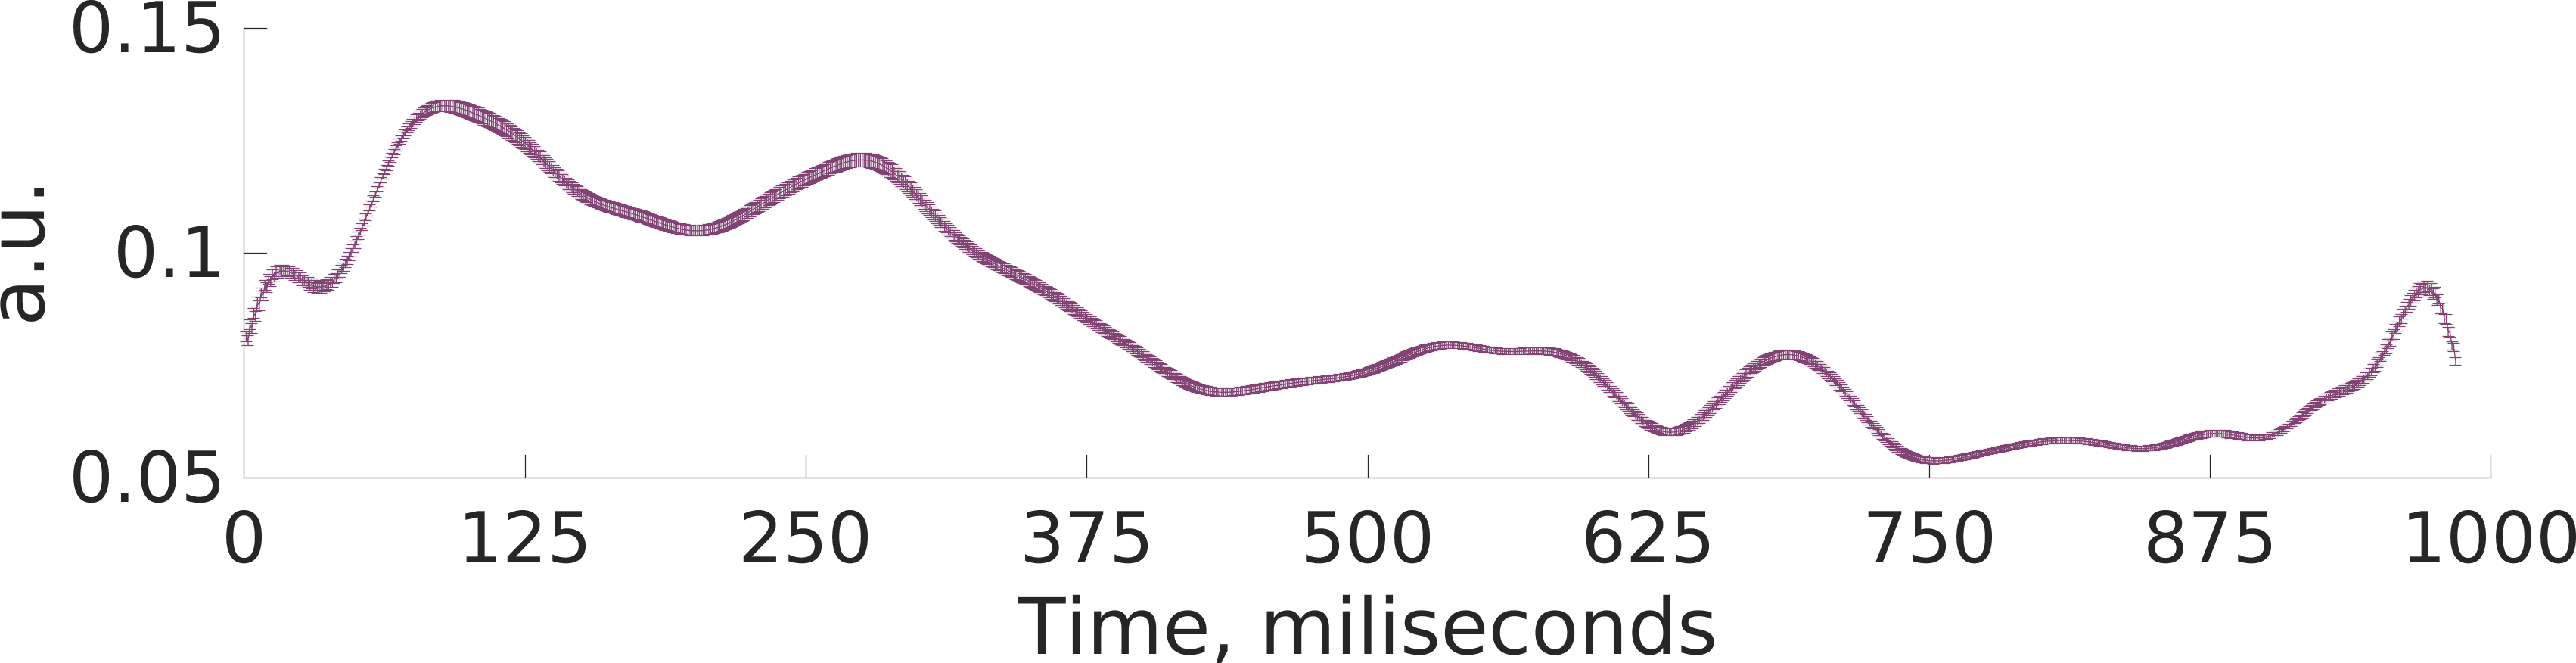
\includegraphics[width=\textwidth]{../images/psiicos_paper/Figure12_a2.jpg}
 \caption{Re, сеть 1}\label{fig:12a}
 \end{subfigure}
 \hspace{1cm}
 \begin{subfigure}[b]{0.4\textwidth}
 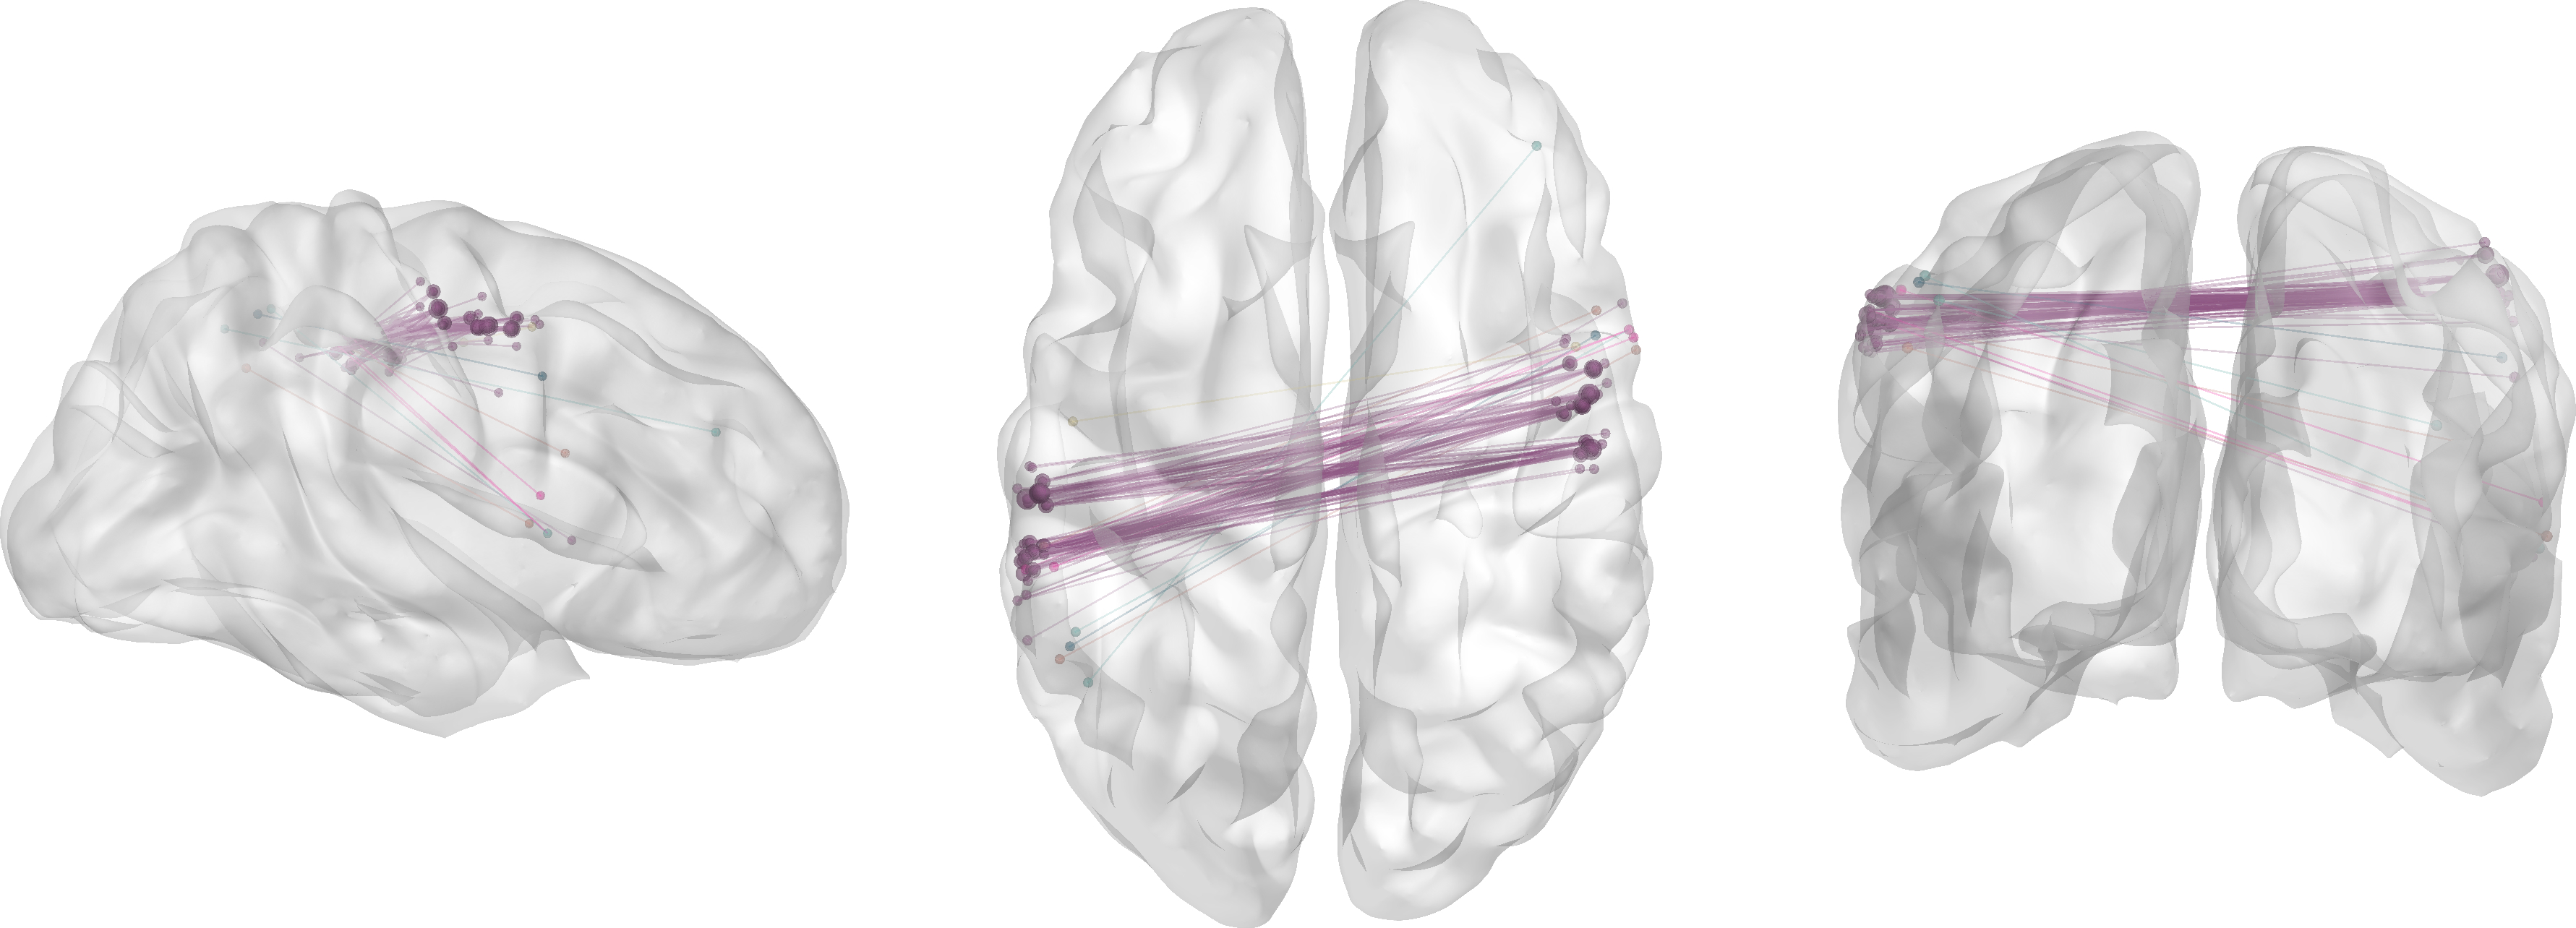
\includegraphics[width=\textwidth]{../images/psiicos_paper/Figure12_b1.jpg}
 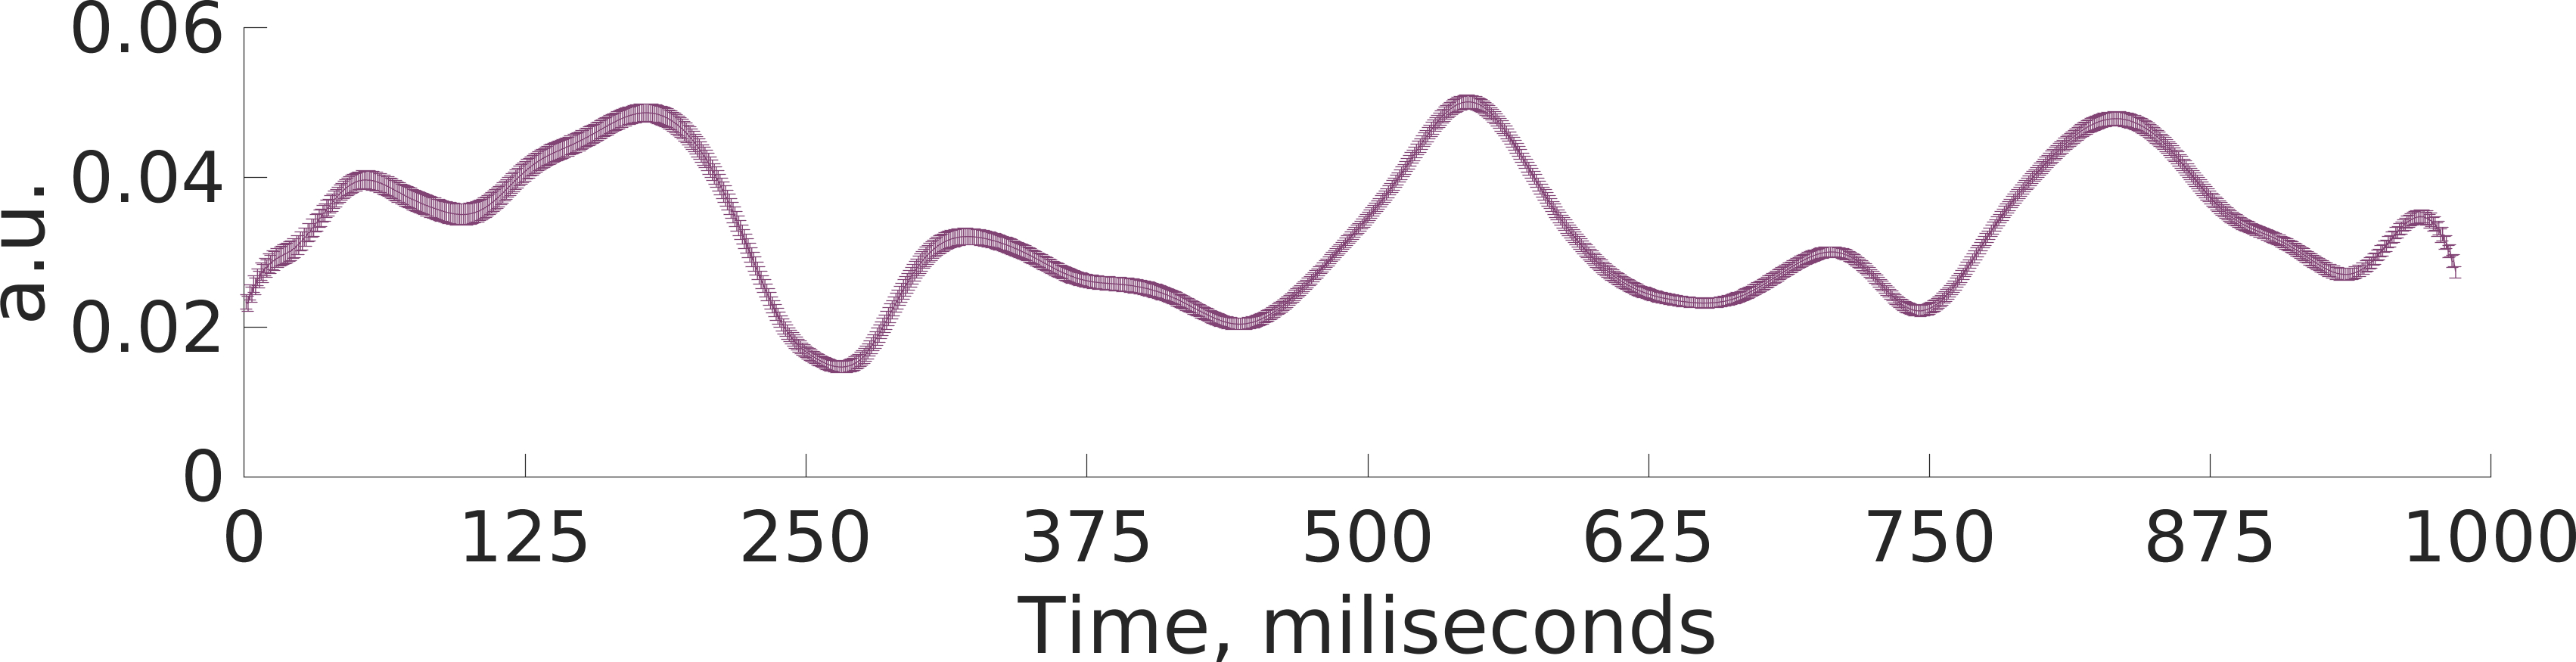
\includegraphics[width=\textwidth]{../images/psiicos_paper/Figure12_b2.jpg}
 \caption{Re, сеть 2}\label{fig:12b}
 \end{subfigure}
 \begin{subfigure}[b]{0.4\textwidth}
 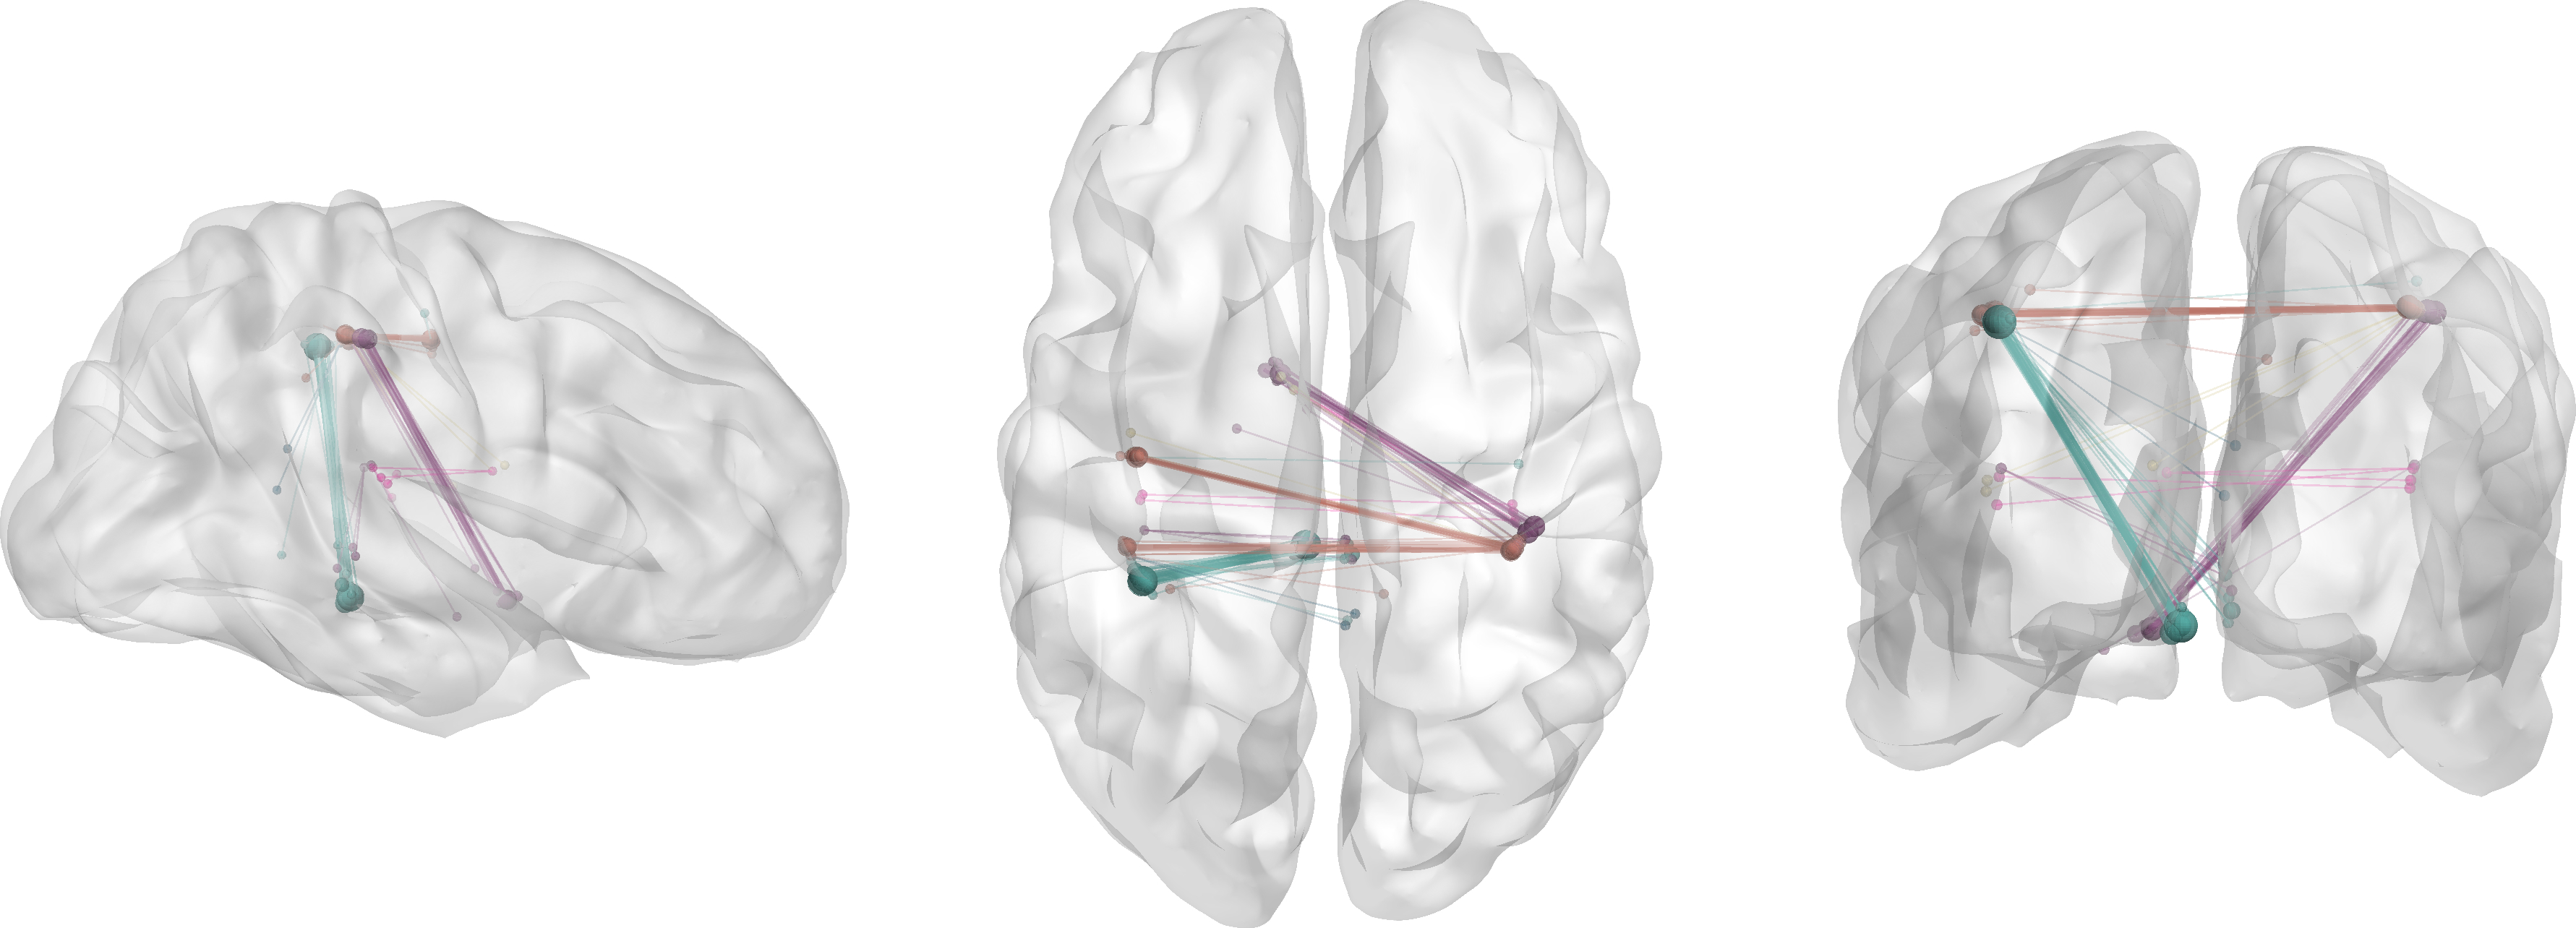
\includegraphics[width=\textwidth]{../images/psiicos_paper/Figure12_c1.jpg}
 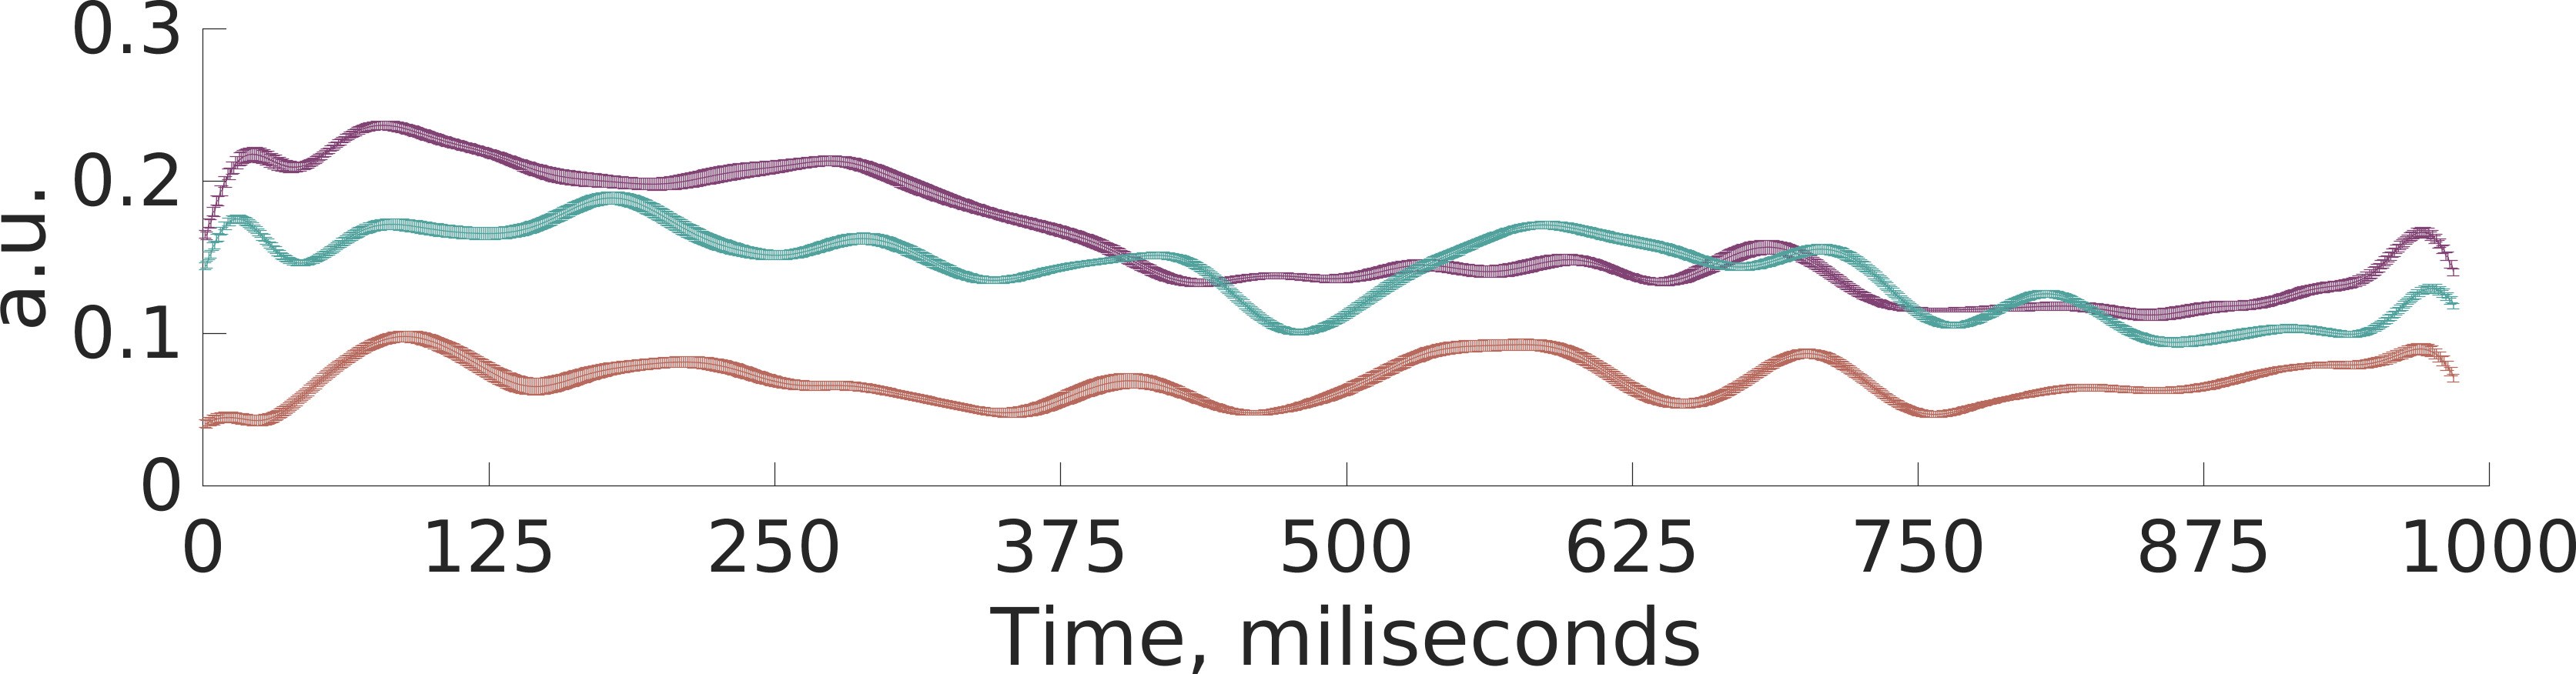
\includegraphics[width=\textwidth]{../images/psiicos_paper/Figure12_c2.jpg}

 \caption{Im, сеть 1}\label{fig:12c}
 \end{subfigure}
 \caption{Пространственная структура и временная динамика наиболее воспроизводимых сетей в бета-диапазоне (16--24 Гц)}\label{fig:12}
\end{figure} %figure 12

\begin{figure}
\centering
\text{Нижний (30--60 Гц) и верхний (65--85 Hz) гамма-диапазоны}

 \begin{subfigure}[b]{0.4\textwidth}
 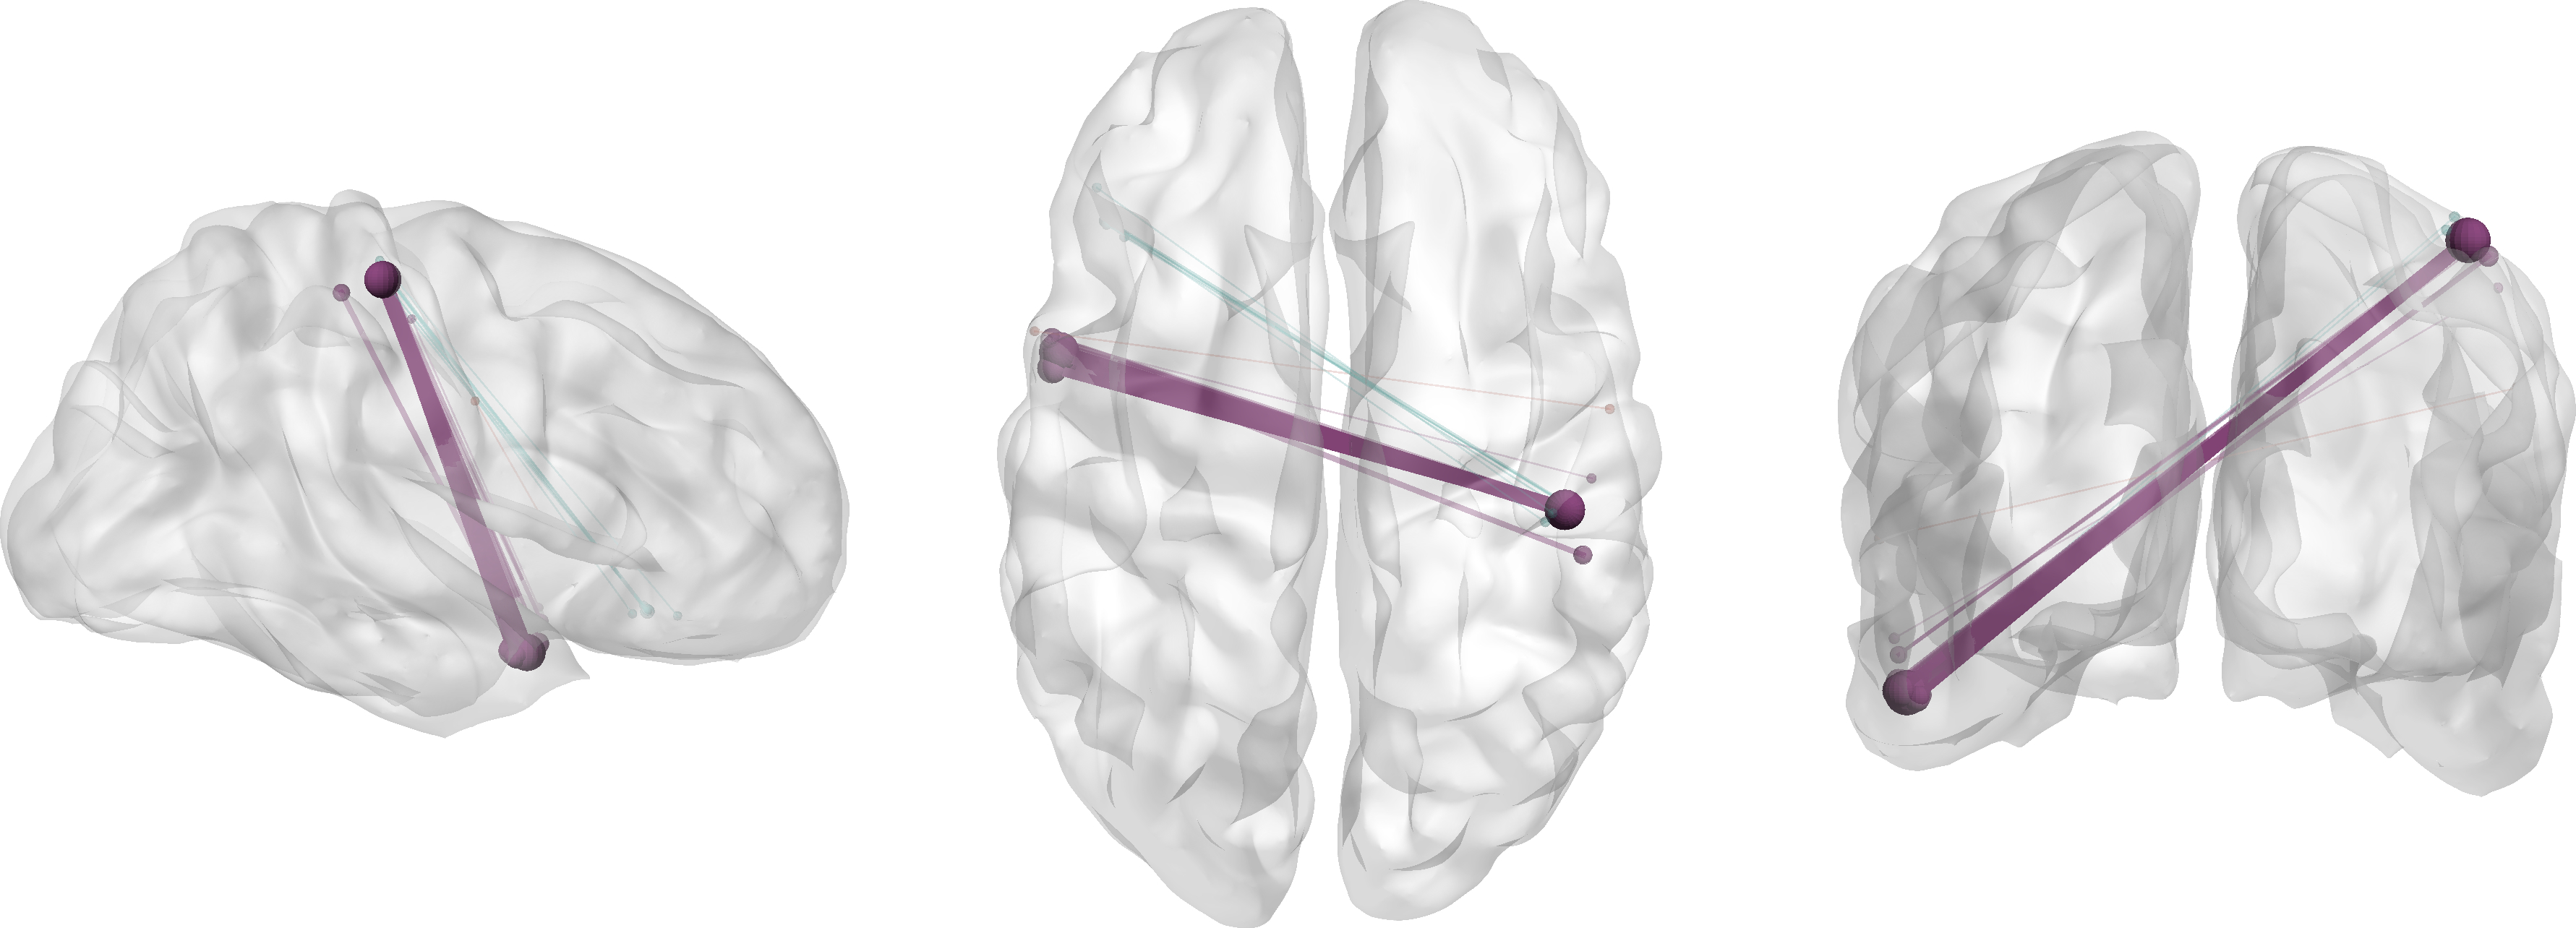
\includegraphics[width=\textwidth]{../images/psiicos_paper/Figure13_a1.jpg}
 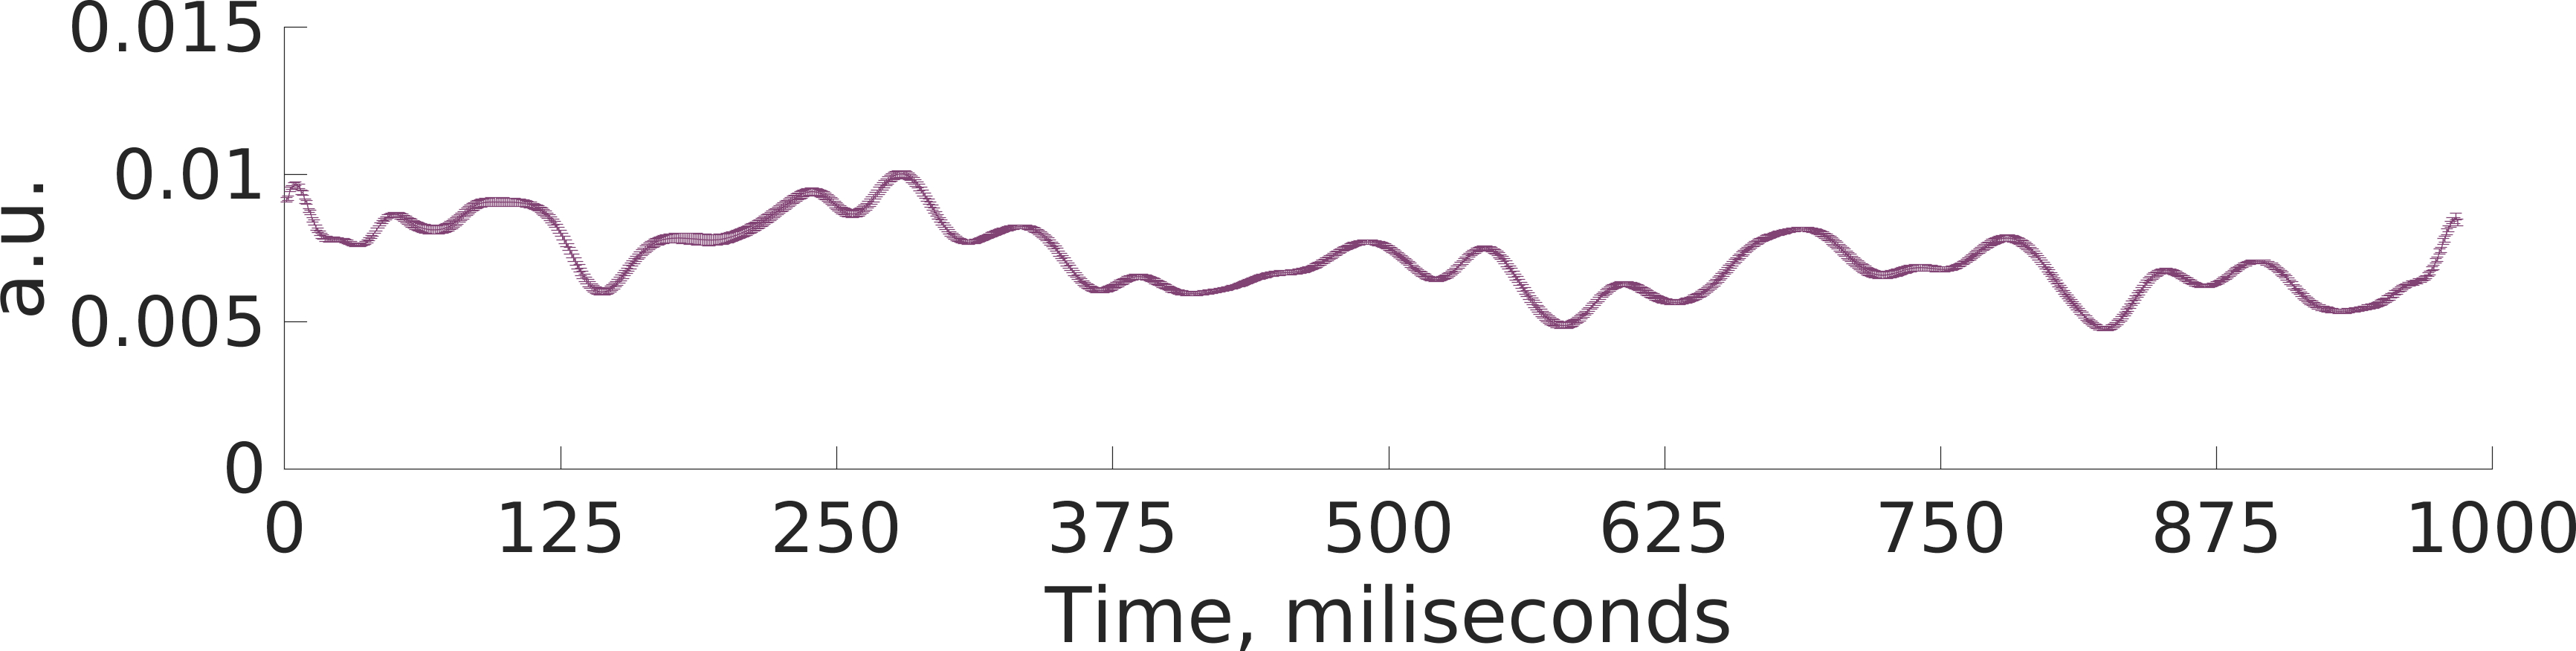
\includegraphics[width=\textwidth]{../images/psiicos_paper/Figure13_a2.jpg}
 \caption{Ниж. гамма-диапазон, Re, сеть 1}\label{fig:13a}
 \end{subfigure}
 \hspace{1cm}
 \begin{subfigure}[b]{0.4\textwidth}
 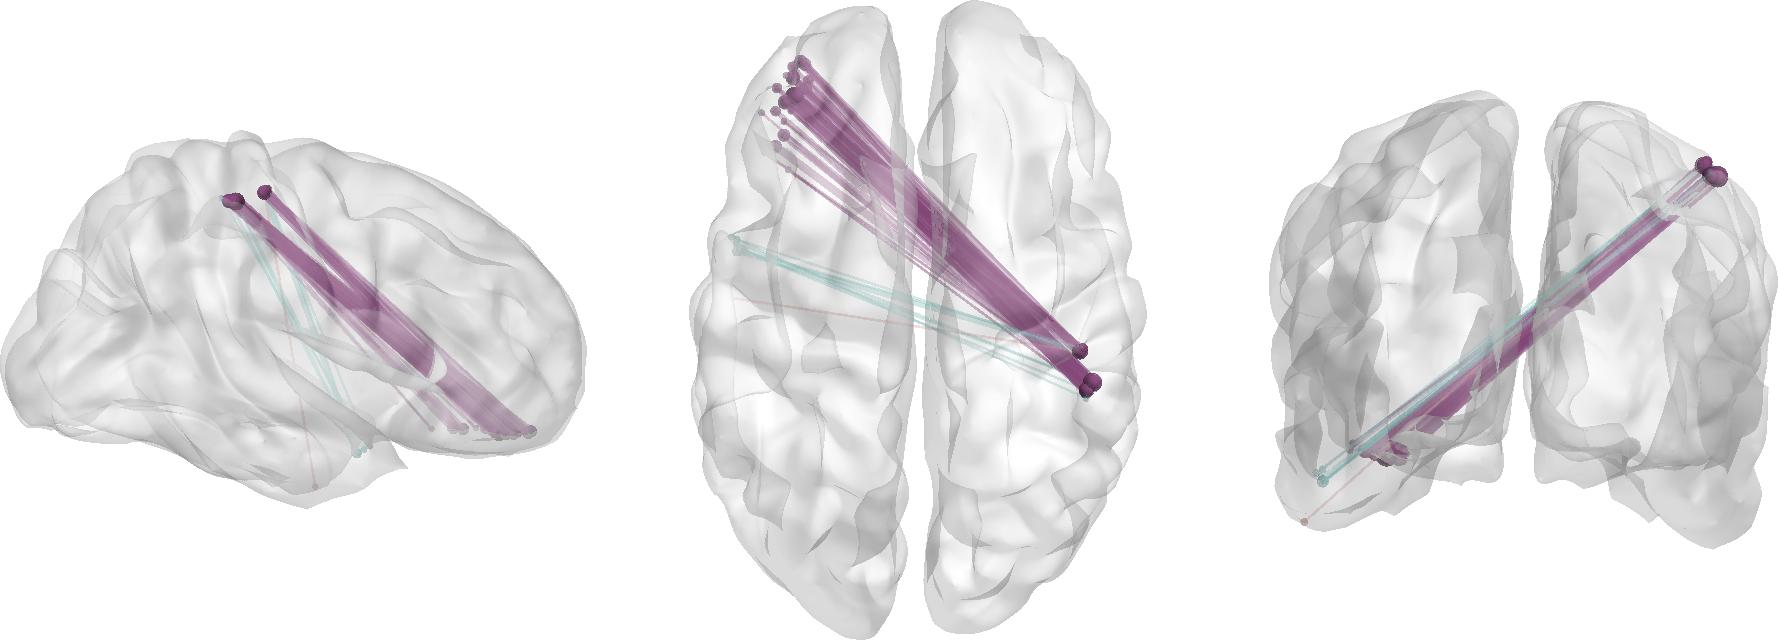
\includegraphics[width=\textwidth]{../images/psiicos_paper/Figure13_b1.jpg}
 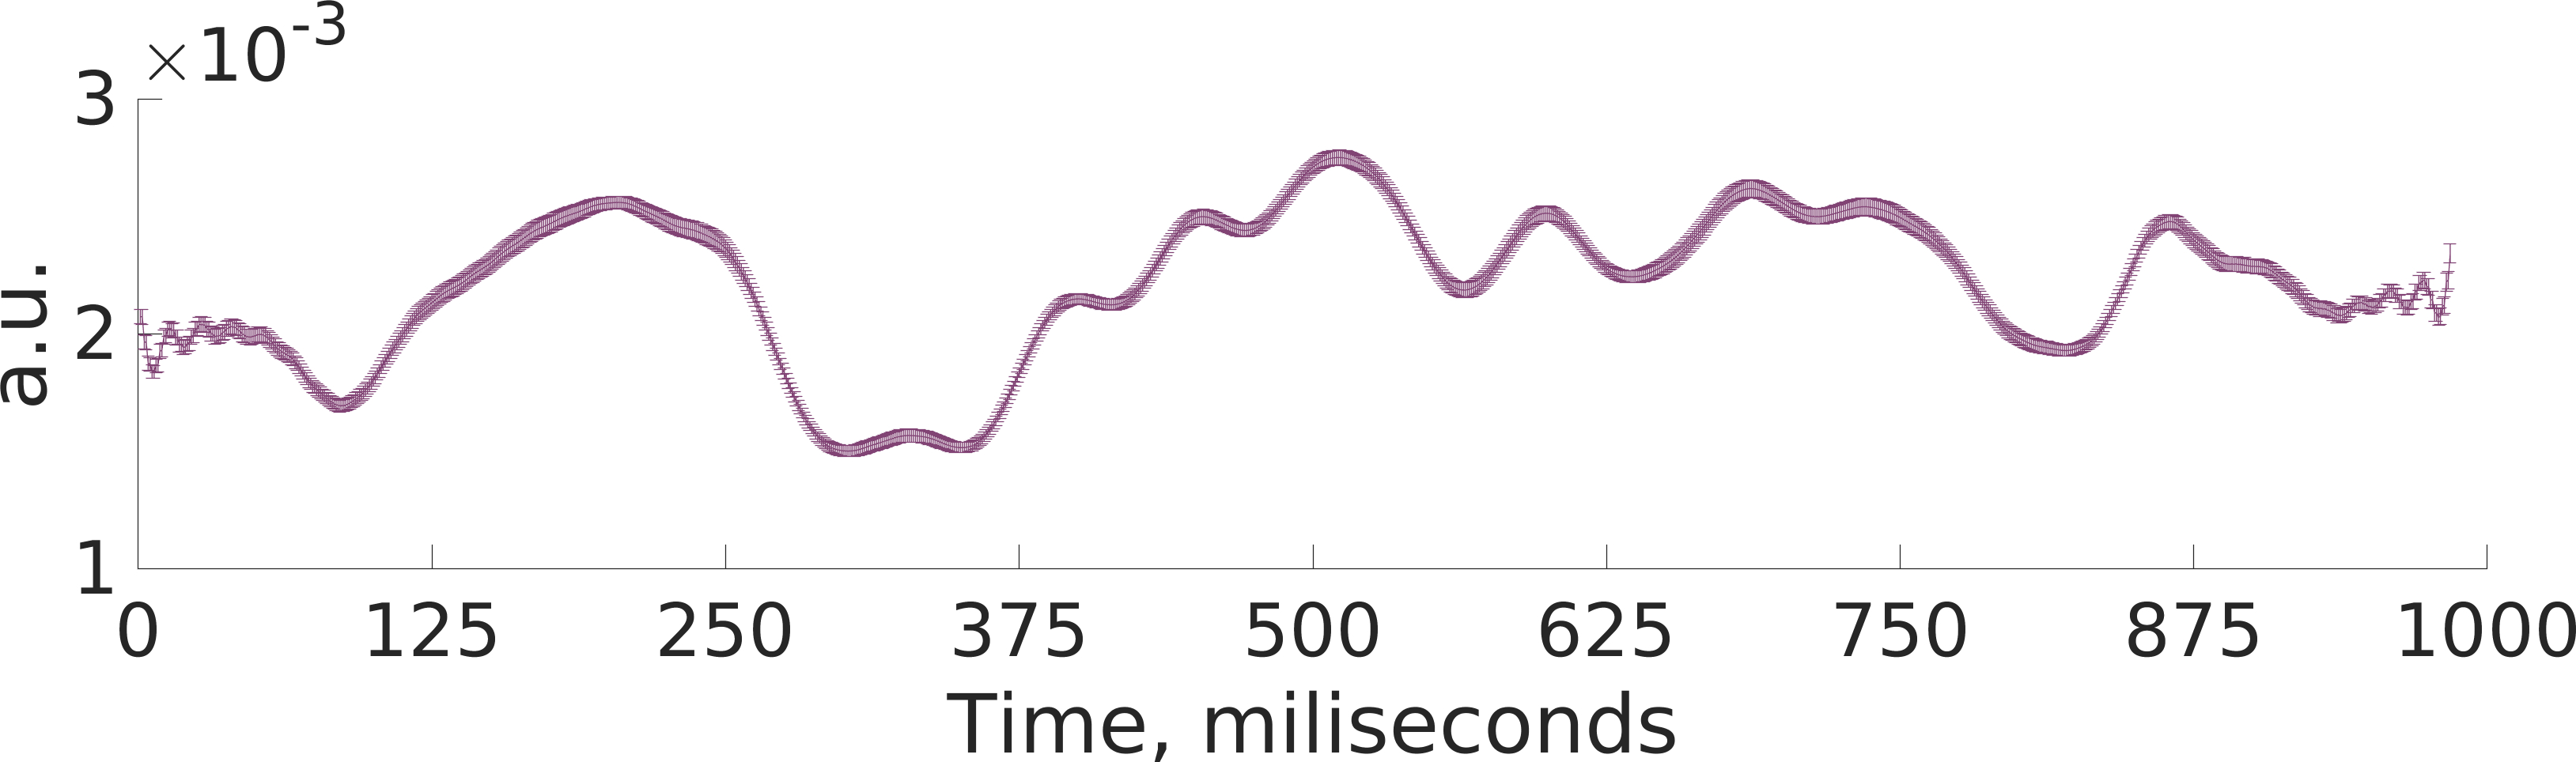
\includegraphics[width=\textwidth]{../images/psiicos_paper/Figure13_b2.jpg}
 \caption{Верх. гамма-диапазон, Re, сеть 1}\label{fig:13b}
 \end{subfigure}

 \begin{subfigure}[b]{0.4\textwidth}
 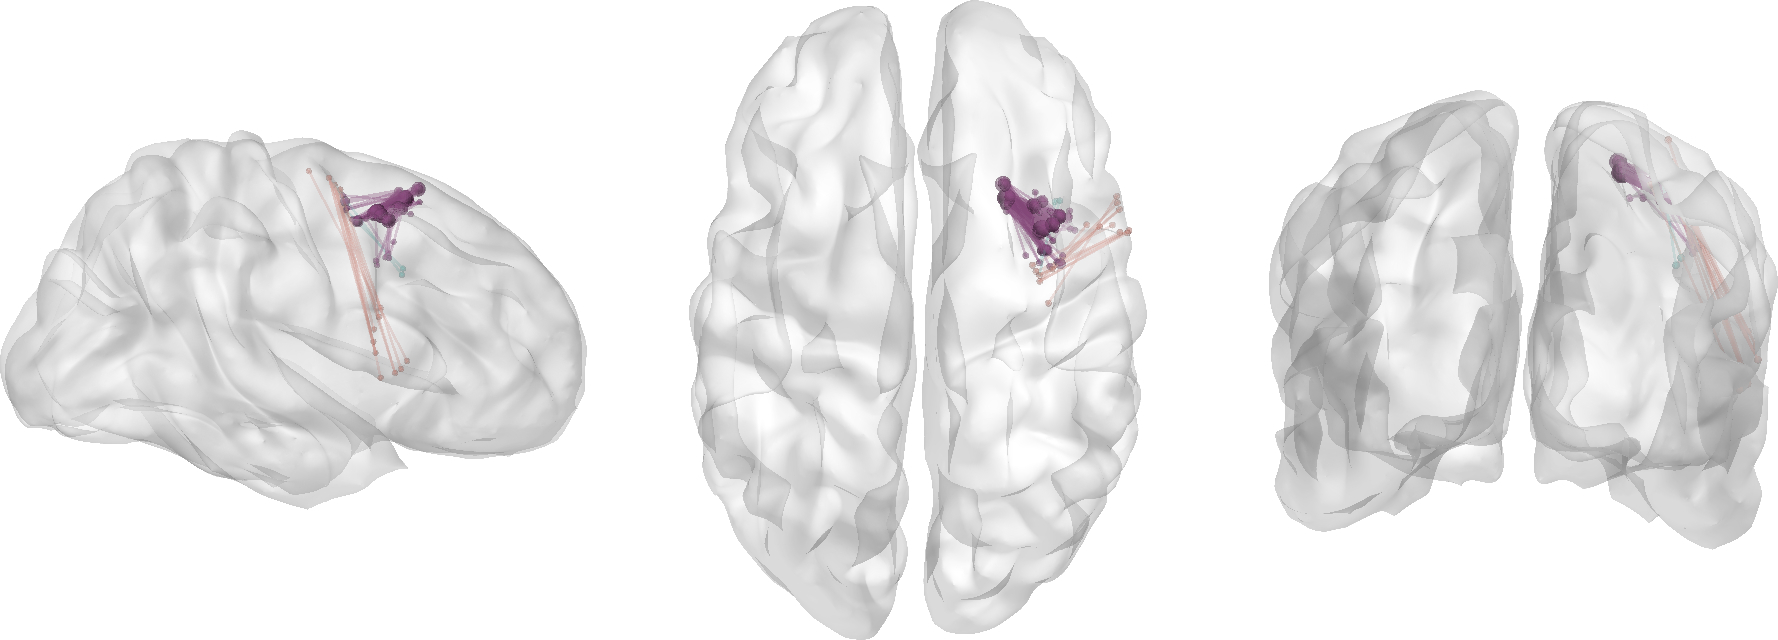
\includegraphics[width=\textwidth]{../images/psiicos_paper/Figure13_c1.jpg}
 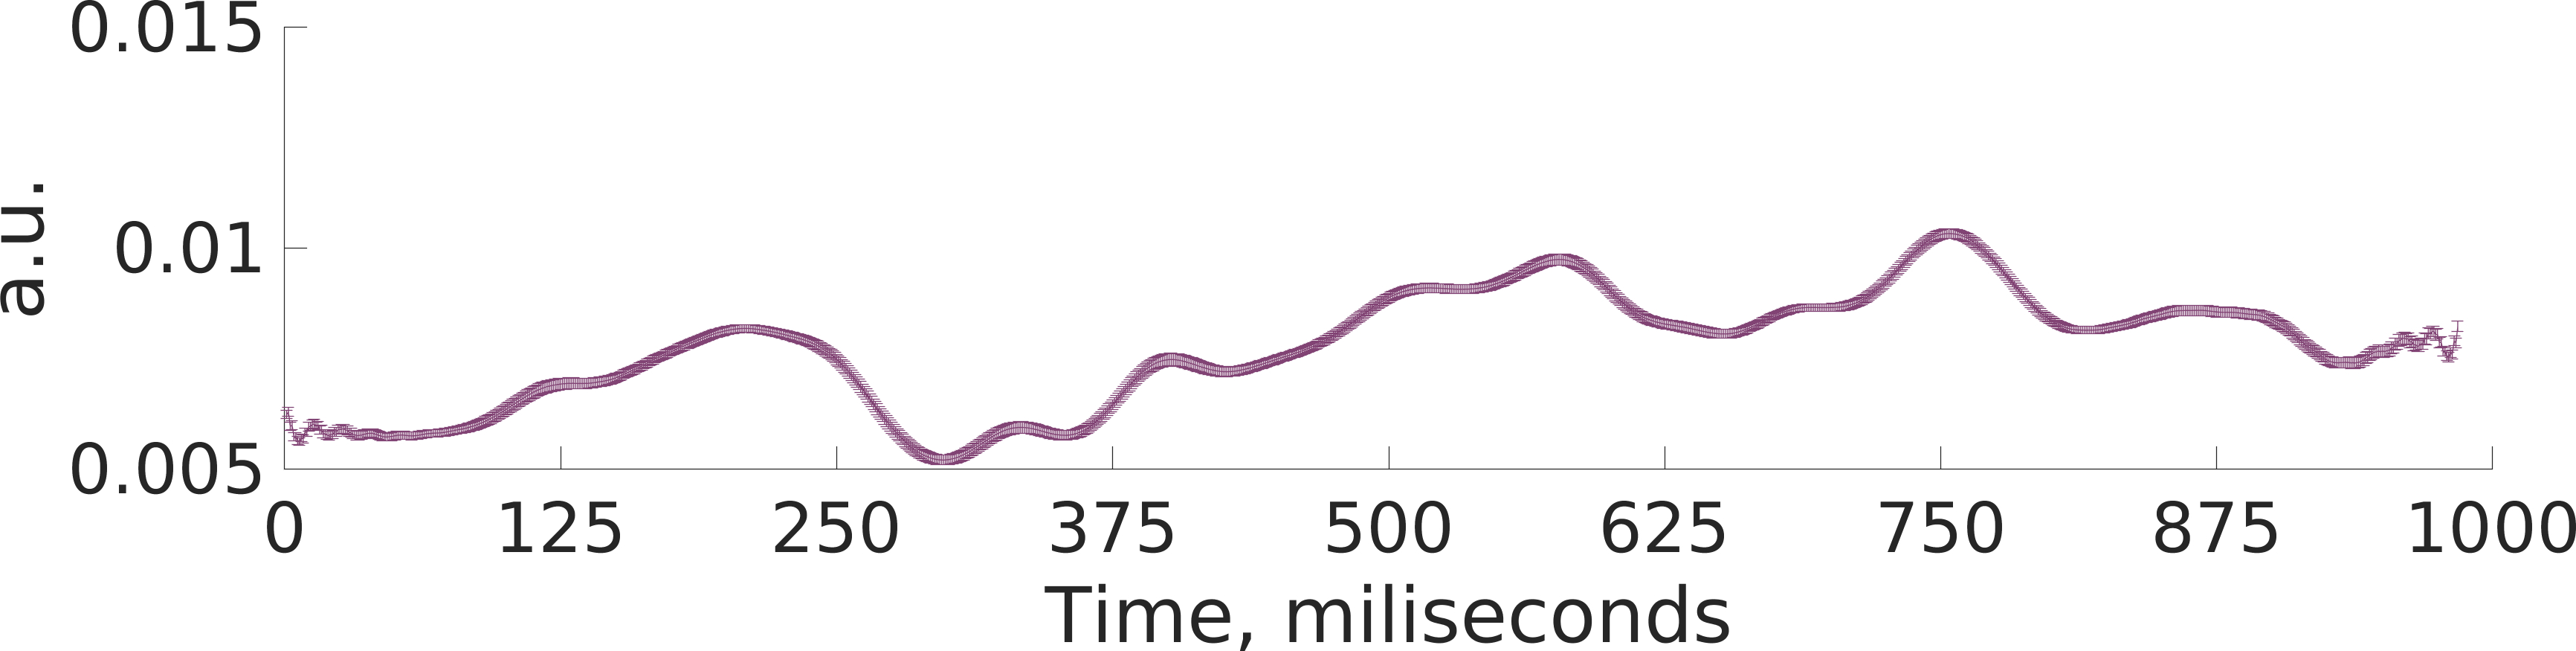
\includegraphics[width=\textwidth]{../images/psiicos_paper/Figure13_c2.jpg}
 \caption{Ниж. гамма-диапазон, Im, сеть 1}\label{fig:13c}
 \end{subfigure}
 \caption{Пространственная структура и временная динамика наиболее воспроизводимых сетей в нижнем (30--60 Гц) и верхнем (65--85 Гц) гамма-диапазонах}\label{fig:13}
\end{figure} % Figure 13

Сети, найденные по мнимой части кросс-спектра, включают связь в альфа-диапазоне
билатеральных сенсорных областей со срединной внутренней поверхностью
коры,~\ref{fig:11b}, а также кросс-латеральные связи между относящимися к руке
зонами сенсорной коры в бета-диапазоне,~\ref{fig:12c}.

Мы также сравнили результаты нашего анализа коннективности с
пространственно-специфичным распределением индуцированной мощности по
коре,~\ref{appendix:real_data_power}. Результаты этого сравнения показывают,
что все обнаруженные сети кроме одной билатеральной сети в бета-диапазоне не
демонстрируют ситуации, когда оба узла сети лежат в областях с высокой
мощностью. В то же время, сенсомоторная область правого полушария, будучи узлом
большинства найденных сетей, совпадает с областью наибольшей активации. Так как
правая мотосенсорная кора играет ключевую роль в исходном
исследовании~\cite{DeLange2008} и так как мы оценивали коннективность не для
одной точки с остальными частями коры, а всех точек со всеми, мы находим эти
результаты обнадеживающими.

\section{Действие проекции на компоненты кросс-спектра в пространстве источников.}\label{sec:subspaces_attenuation}

Из-за ортогональности 2-топографий действительной и мнимой частей операция
проекции никак не влияет на мнимую часть кросс-спектра. На действительную
часть, содержащую информацию о малых фазовых задержках, проекция напротив
оказывыает значительное влияние.  Удаляя часть, соответствующую протечке
сигнала, мы неизбежно удаляем и часть полезного сигнала. Качество работы
предложенного алгоритма подавления протечки сигнала в действительной части
кросс-спектра существенно зависит от следующих двух факторов:

\begin{itemize}
    \item PSIICOS-проекция должна максимально подавлять мощность компонент в
        подпространстве протечки сигнала и одновременно с этим минимально
        изменять мощность истинной действительной части когеренции.
    \item Как и для всех алгоритмов решения обратной задачи PSIICOS-проекция
        существенно зависит от точности прямой модели. Неизбежная погрешность
        при ее построении~\cite{Mosher1999} оказывает соответствующее влияние
        на качество решений предложенного метода. Вместе с тем, ошибки прямой
        модели в разумных пределах должны вызывать лишь незначительное
        ухудшение качества решения.
\end{itemize}

Степень выполнения этих условий зависит от феноменологических характеристик
массива сенсоров, а также от магнитных топографий имеющихся мозговых
источников. В этом разделе мы опишем результаты численного моделирования,
направленного на изучение этой проблемы.

Подавление мощности в подпространстве действительной части кросс-спектра
очевидным образом проявляется наиболее сильно для источников с кореллированными
топографиями.  Для исследования зависимости подавления от коэффициента
корреляции между топографиями взаимодействующих источников для каждой пары
индексов $i, j$ мы вычисляли нормы до и после проекции для 2-топографий вида
$\vec{g}_i \otimes \vec{g}_i + \vec{g}_j \otimes \vec{g}_j$,
$\vec{g}_j\otimes\vec{g}_i + \vec{g}_i\otimes\vec{g}_j$ а также
$\vec{g}_j\otimes\vec{g}_i - \vec{g}_i\otimes\vec{g}_j$, соответствующие
подпространствам $S^{SL}, S^{\Im}, S^{\Re}$. Результаты представлены на графике~\ref{fig:02}.

\begin{figure}[!ht]
 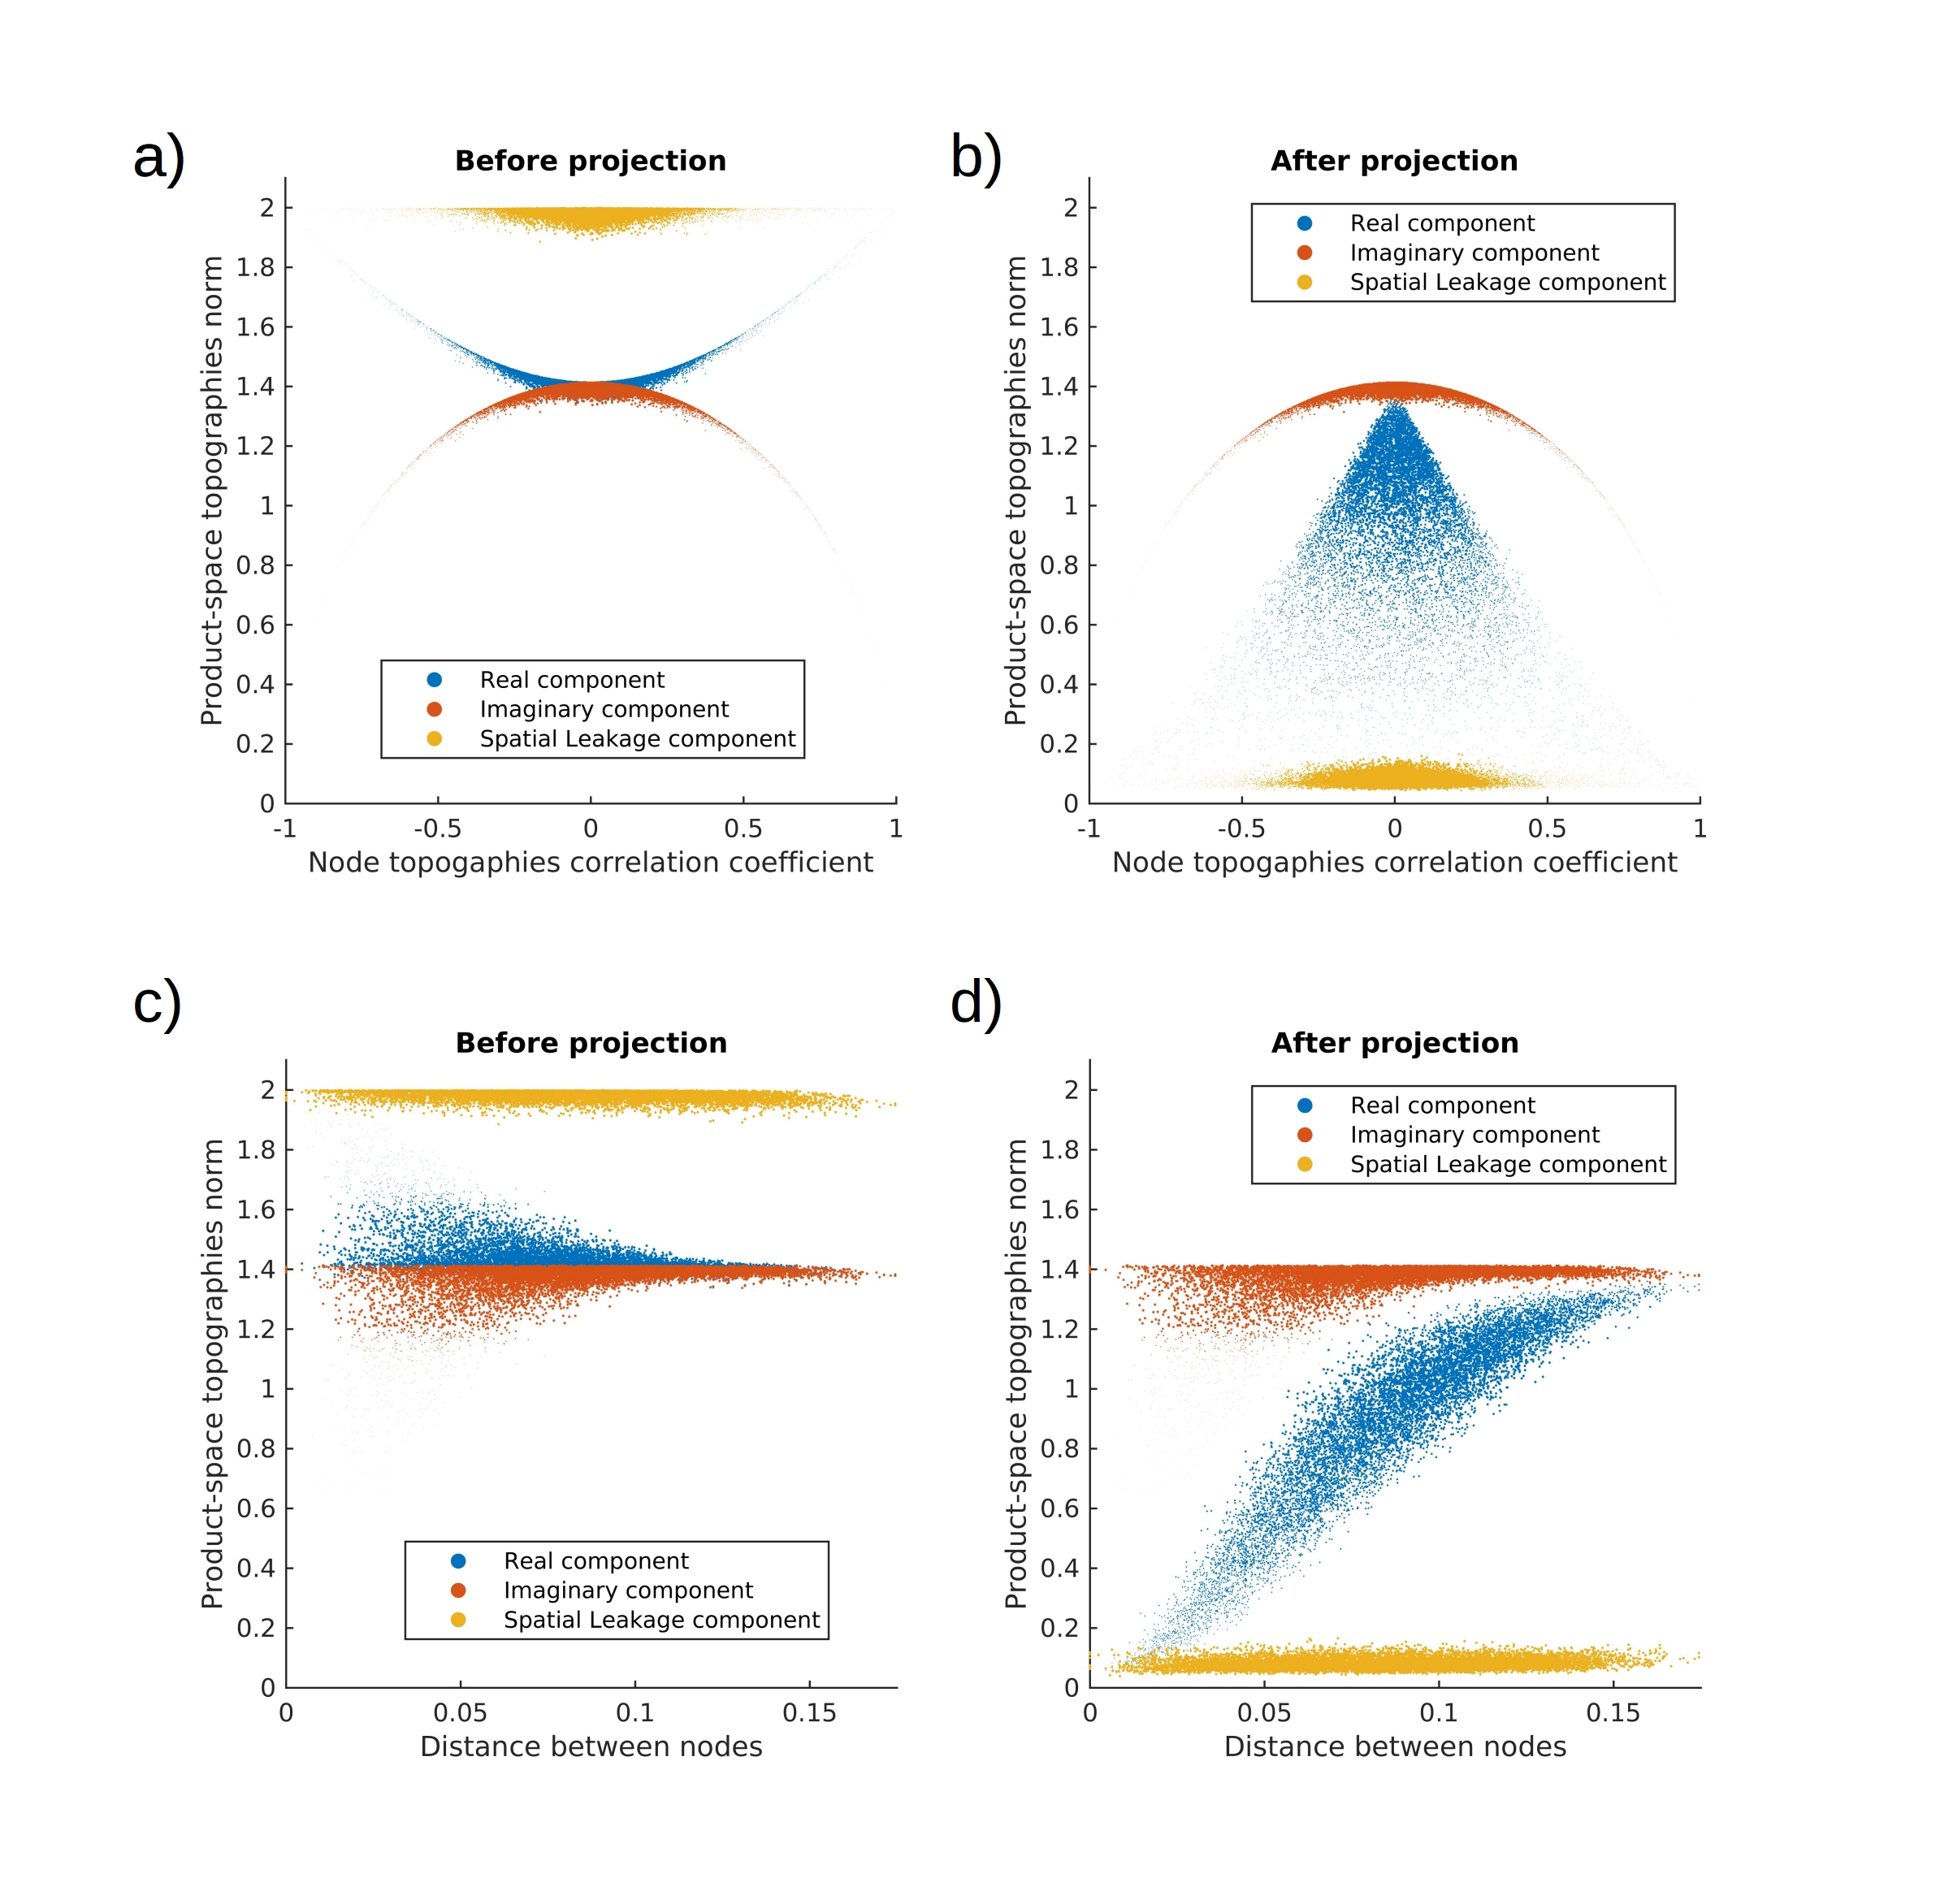
\includegraphics[width=1\textwidth]{../images/psiicos_paper/Figure3abcd_hr}
 \caption{Нормы 2-топографий для трех подпространств кросс-спектра до и после проекци
     в зависимости от коэффициента корреляции топографий взаимодействующих
     узлов на коре (графики (a) и (b)), а также от расстояния между
     этими узлами (графики (c) и (d)).}\label{fig:02} % Figure 3 in the text
     До проекции (графики (a), (c)) в кросс-спектр на уровне сенсоров наибольший вклад дает мощностная
     компонента (обозначена желтым цветом). После проекции (графики (b), (d))
     вклад мощностной компоненты уменьшается в среднем в 25 раз. Вместе с
     тем наблюдается неизбежное, но значительно меньшее ослабление
     2-топографий действительной части, соответствующих истинной коннективности.
     В среднем они ослабляются в 1.6 раз.
\end{figure}

Для каждой сети с узлами в точках $i$ и $j$ на коре соответствует три точки
разных цветов на графике: красная, синяя и желтая. Градации синего цвета мы
использовали для кодировки информации о величине нормы 2-топографии
действительной части $\vec{g}_j\otimes\vec{g}_i + \vec{g}_i\otimes\vec{g}_j$.
Градации красного цвета использовались для 2-топографий мнимой части, и
желтого~--- для топографий протечки сигнала.  Положение каждой цветной точки
вдоль оси $x$ для подграфиков (a), (b) определялось величной коэффициента
корреляции топографий $\vec{g}_i$ и $\vec{g}_j$.  Кроме того, мы отобразили те
же самые данные на втором графике, где вместо корреляции по оси $x$
использовалось расстояние между узлами сети $i, j$. Насыщенность цвета точек
отражает плотность точек в соответствующей области графика.

\section{Выбор ранга проекции}\label{subsec:rank_impact}

Мы изучили зависимость коэффициентов ослабления подпространствах протечки
сигнала, а также мнимой и действительной части в зависимости от ранга проекции.
На рисунке~\ref{fig:14} показано среднее затухание мощности в трех
подпространствах в зависимости от ранга проекции.

На практике для ускорения расчетов при обработке МЭГ-данных часто пользуются
методом главных компонент для сокращения размерности пространства сенсоров.
Различные кривые на графике показывают, каким образом ведет себя PSIICOS-проекция
для разных рангов при таком сокращении размерности.

Чтобы получить этот график, мы использовали симуляции Монте-Карло.
На каждой итерации мы случайным образом выбирали подмножество из 200 источников
и вычисляли все 2-топографии из трех подпространств $S_{SL}, S_{\Re}, S_{\Im}$.
Мы использовали источники с фиксированными ориентациями, ортогональными к поверхности коры.
Затем мы изменяли ранг проекции и вычисляли спроецированные версии 2-топографий этих сетей.
Для количественной оценки эффекта затухания мы рассчитывали среднее отношение
норм исходных и спроецированных 2-топографий для каждого значения ранга проекции.
Этот процесс мы повторили 100 раз и усреднили результат.

Из-за пересечения подпространств $S_{SL}$ и $S_{\Re}$ операция проецирования
стремится подавить мощность компоненты SL, что неизбежно приводит к подавлению
мощности в подпространстве $S_{\Re}$.  Чем меньше мощность в подпространстве
$S_{\Re}$ подавляется для фиксированного коэффициента подавления мощности в
$S_{SL}$, тем выше итоговое качество решения. Поэтому в дополнение к кривым
затухания для подпространств мы также нанесли логарифм отношения коэффициентов
ослабления, наблюдаемых для векторов в подпространстве $S_{\Re}$, к векторам в
подпространстве $S_{SL}$. Использование SVD-разложения при формировании
оператора проекции делает возможным значительно более быстрое уменьшение
мощности в подпространстве протечки сигнала $S_{SL}$, чем в подпространстве $
S_{\Re}$. Другими словами мы видим, что увеличение ранга проекции приводит к
все большему доминированию мощности в подпространстве $S_{\Re}$ по сравнению с
подпространством $S_{SL}$.

\begin{figure}[htbp]
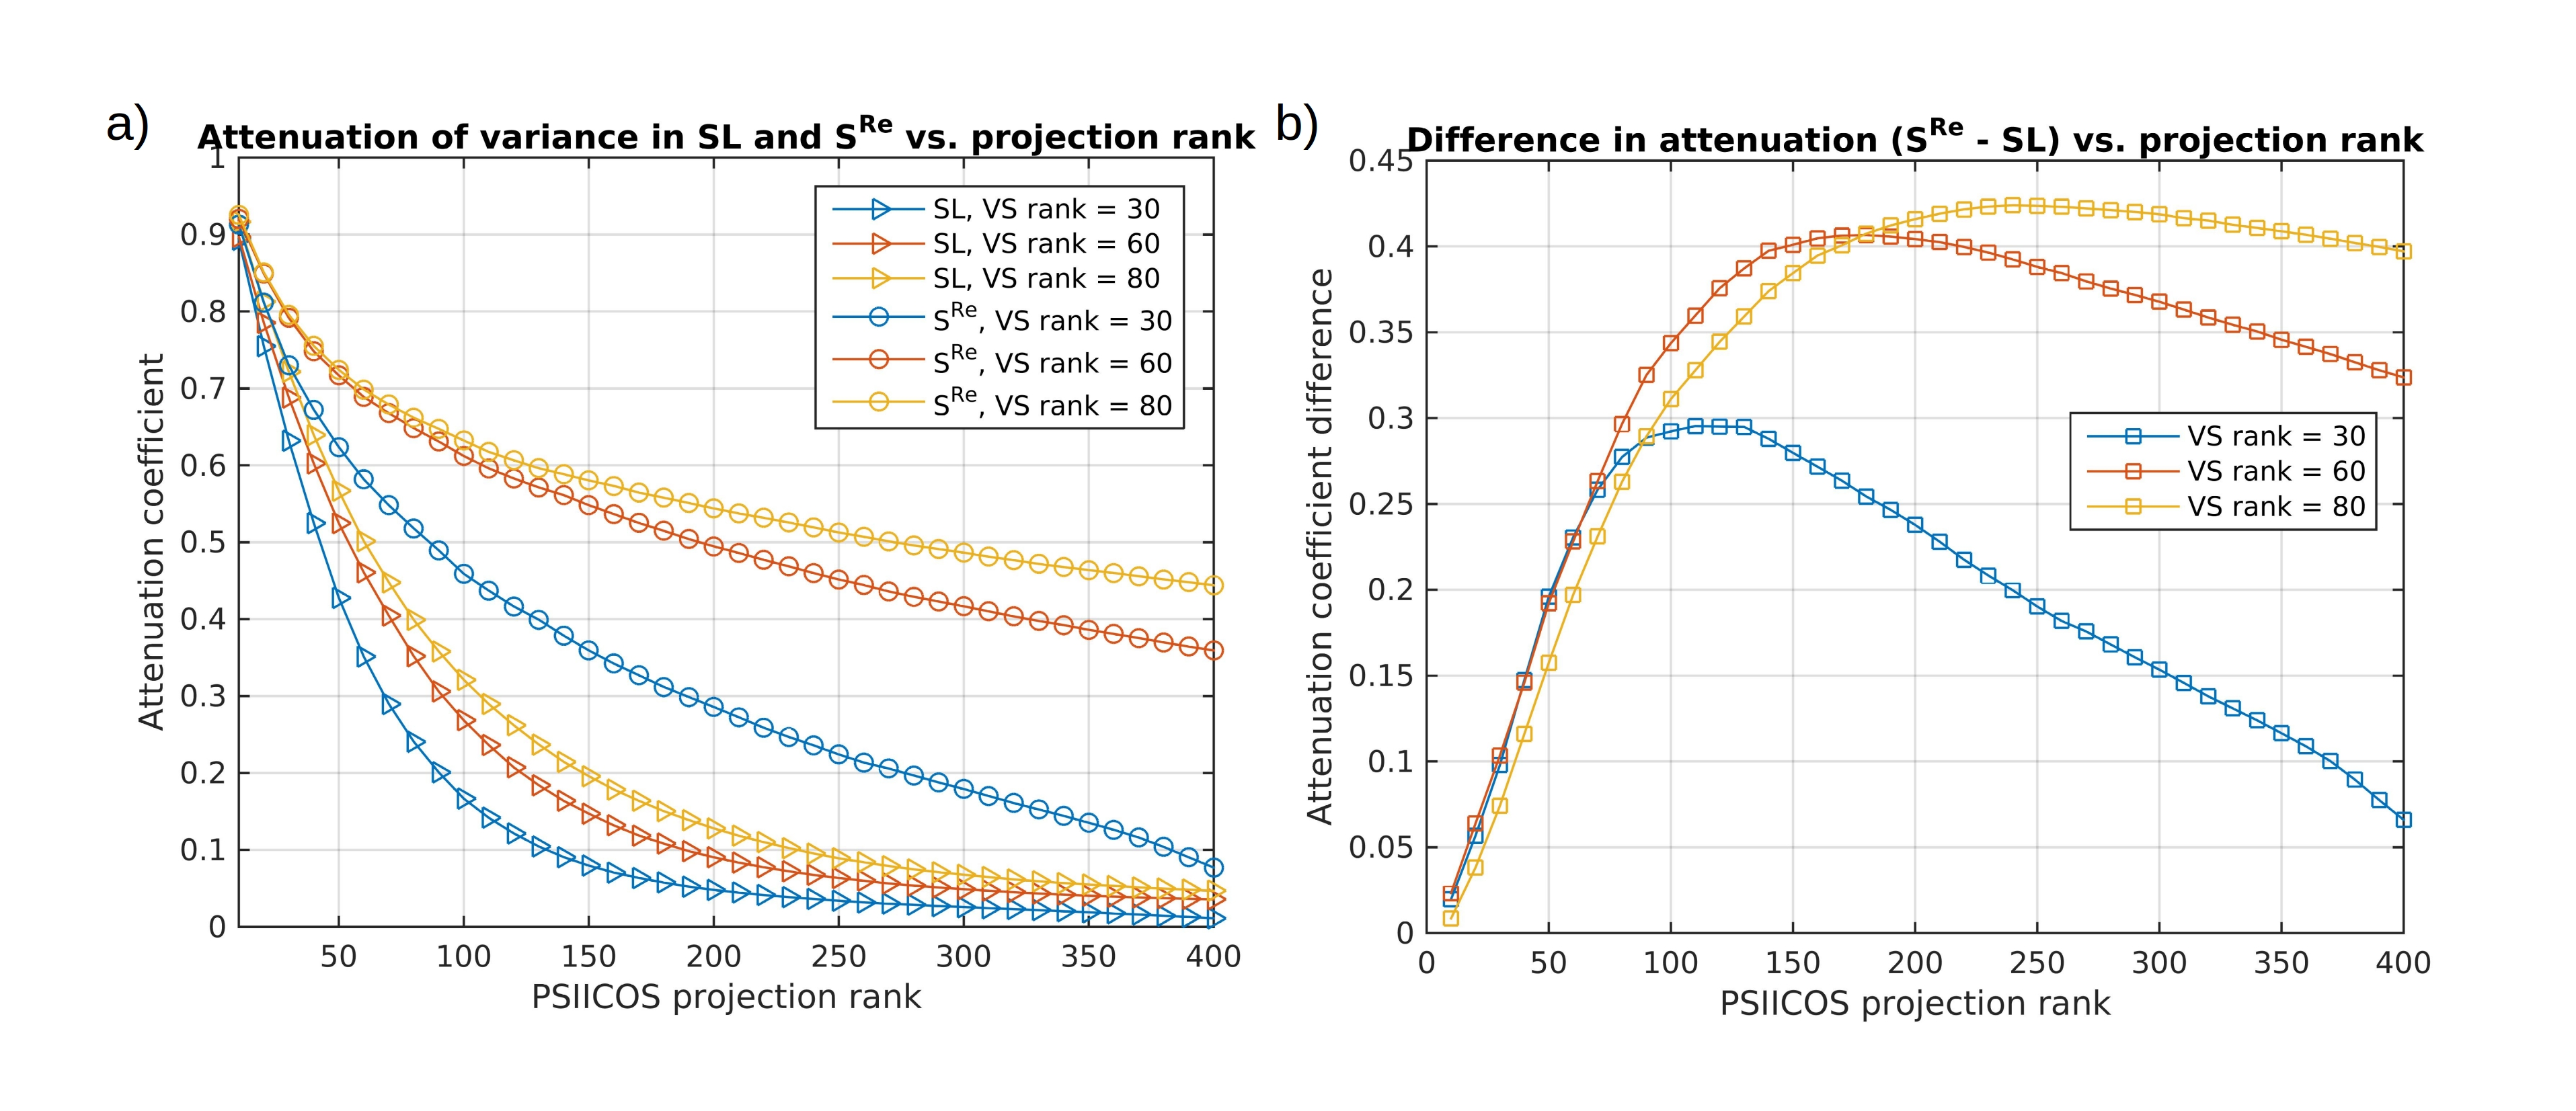
\includegraphics[width=\textwidth]{../images/psiicos_paper/Figure14_hr.jpg}
\caption{(a) Ослабление мощности в подпространствах $S_{SL}$ и $S_{Re}$ и (b)
    Разница в коэффициенте затухания для подпространств $S_{Re}$ и $S_{SL}$ как
    функции ранга проекции для трех различных размерностей пространства виртуальных
    сенсоров (VS).
}\label{fig:14}
    Эти кривые позволяют принять обоснованное решение
    относительно выбора ранга проекции.  Мы предлагаем выбирать такое значение ранга
    проекции PSIICOS, которое соответствует наибольшей разнице в затухании
    мощности.
\end{figure}

\section{Влияние неточностей прямой модели на качество решений}\label{sec:forward_model_errors_effect}

Описанная проекция строится на основании прямой модели, которая в реальных
условиях неизбежно содержит к неточностям.  В этом разделе мы изучили
эффективность предложенной операции проецирования при наличии структурированных
и неструктурированных ошибок в прямой модели.

В этом исследовании мы использовали две различные модели шума.  Первая модель
соответствовала пространственно неструктурированному шуму и была реализована
путем добавления масштабированного случайного шума к матрице прямой модели.

Чтобы получить матрицу реализации шума при оценке прямой модели, мы
сэмплировали данные из стандартного нормального распределения $N(0,1)$.  Далее
мы нормировали эти данные умножением элементов матрицы шума на квадратный корень
из среднего значения следа матрицы $\matr{G}\matr{G}^T$, где
$\matr{G}$~--- матрица прямой модели. Затем мы добавляли эту матрицу к
истинной прямой модели и корректировали количество шума с помощью
параметра $\alpha$.

Вторая модель соответствовала более реалистичному сценарию пространственно
структурированного искажения.  Для генерации пространственно структурированной
шумовой матрицы мы использовали модели головы, рассчитанные для $N=10$
испытуемых, и посчитали разницу между прямыми моделями для каждой пары
субъектов. Мы вычисляли матрицу структурированного шума как среднее из этих
попарных разниц. Затем мы нормировали полученную матрицу структурированного
шума и добавляли ее к истинной прямой модели. Как и в предыдущем случае, мы
регулировали количество шума с помощью параметра $\alpha$.

Потенциально неточности прямой модели могут привести к одновременному
уменьшению ослабления мощности подпространства протечки сигнала и уменьшению
мощности подпространства $S_{\Re}$.  Мы использовали симуляции Монте-Карло для
численного изучения этих эффектов.  На каждой итерации мы случайным образом
выбирали подмножество из 200 источников и рассчитывали средний коэффициент
ослабления для трех подпространств.  Мы сделали это как для случая
структурированного, так и для неструктурированного шума, а также для двух разных
значений ранга проекции (350 и 500). Результаты представлены на рисунке~\ref{fig:15}.

Мы можем видеть, что хотя неточности в прямой модели приводят к
ухудшению работы предлагаемого метода проекции, для типичных уровней
шума в прямой модели для MEG порядка 10 \% (\cite{Mosher1999}) мы имеем почти одинаковое значение
подавления мощности в подпространстве протечки сигнала и только около 20 \% дополнительного уменьшения мощности
в подпространстве $S_{\Re}$.

\begin{figure}[htbp]
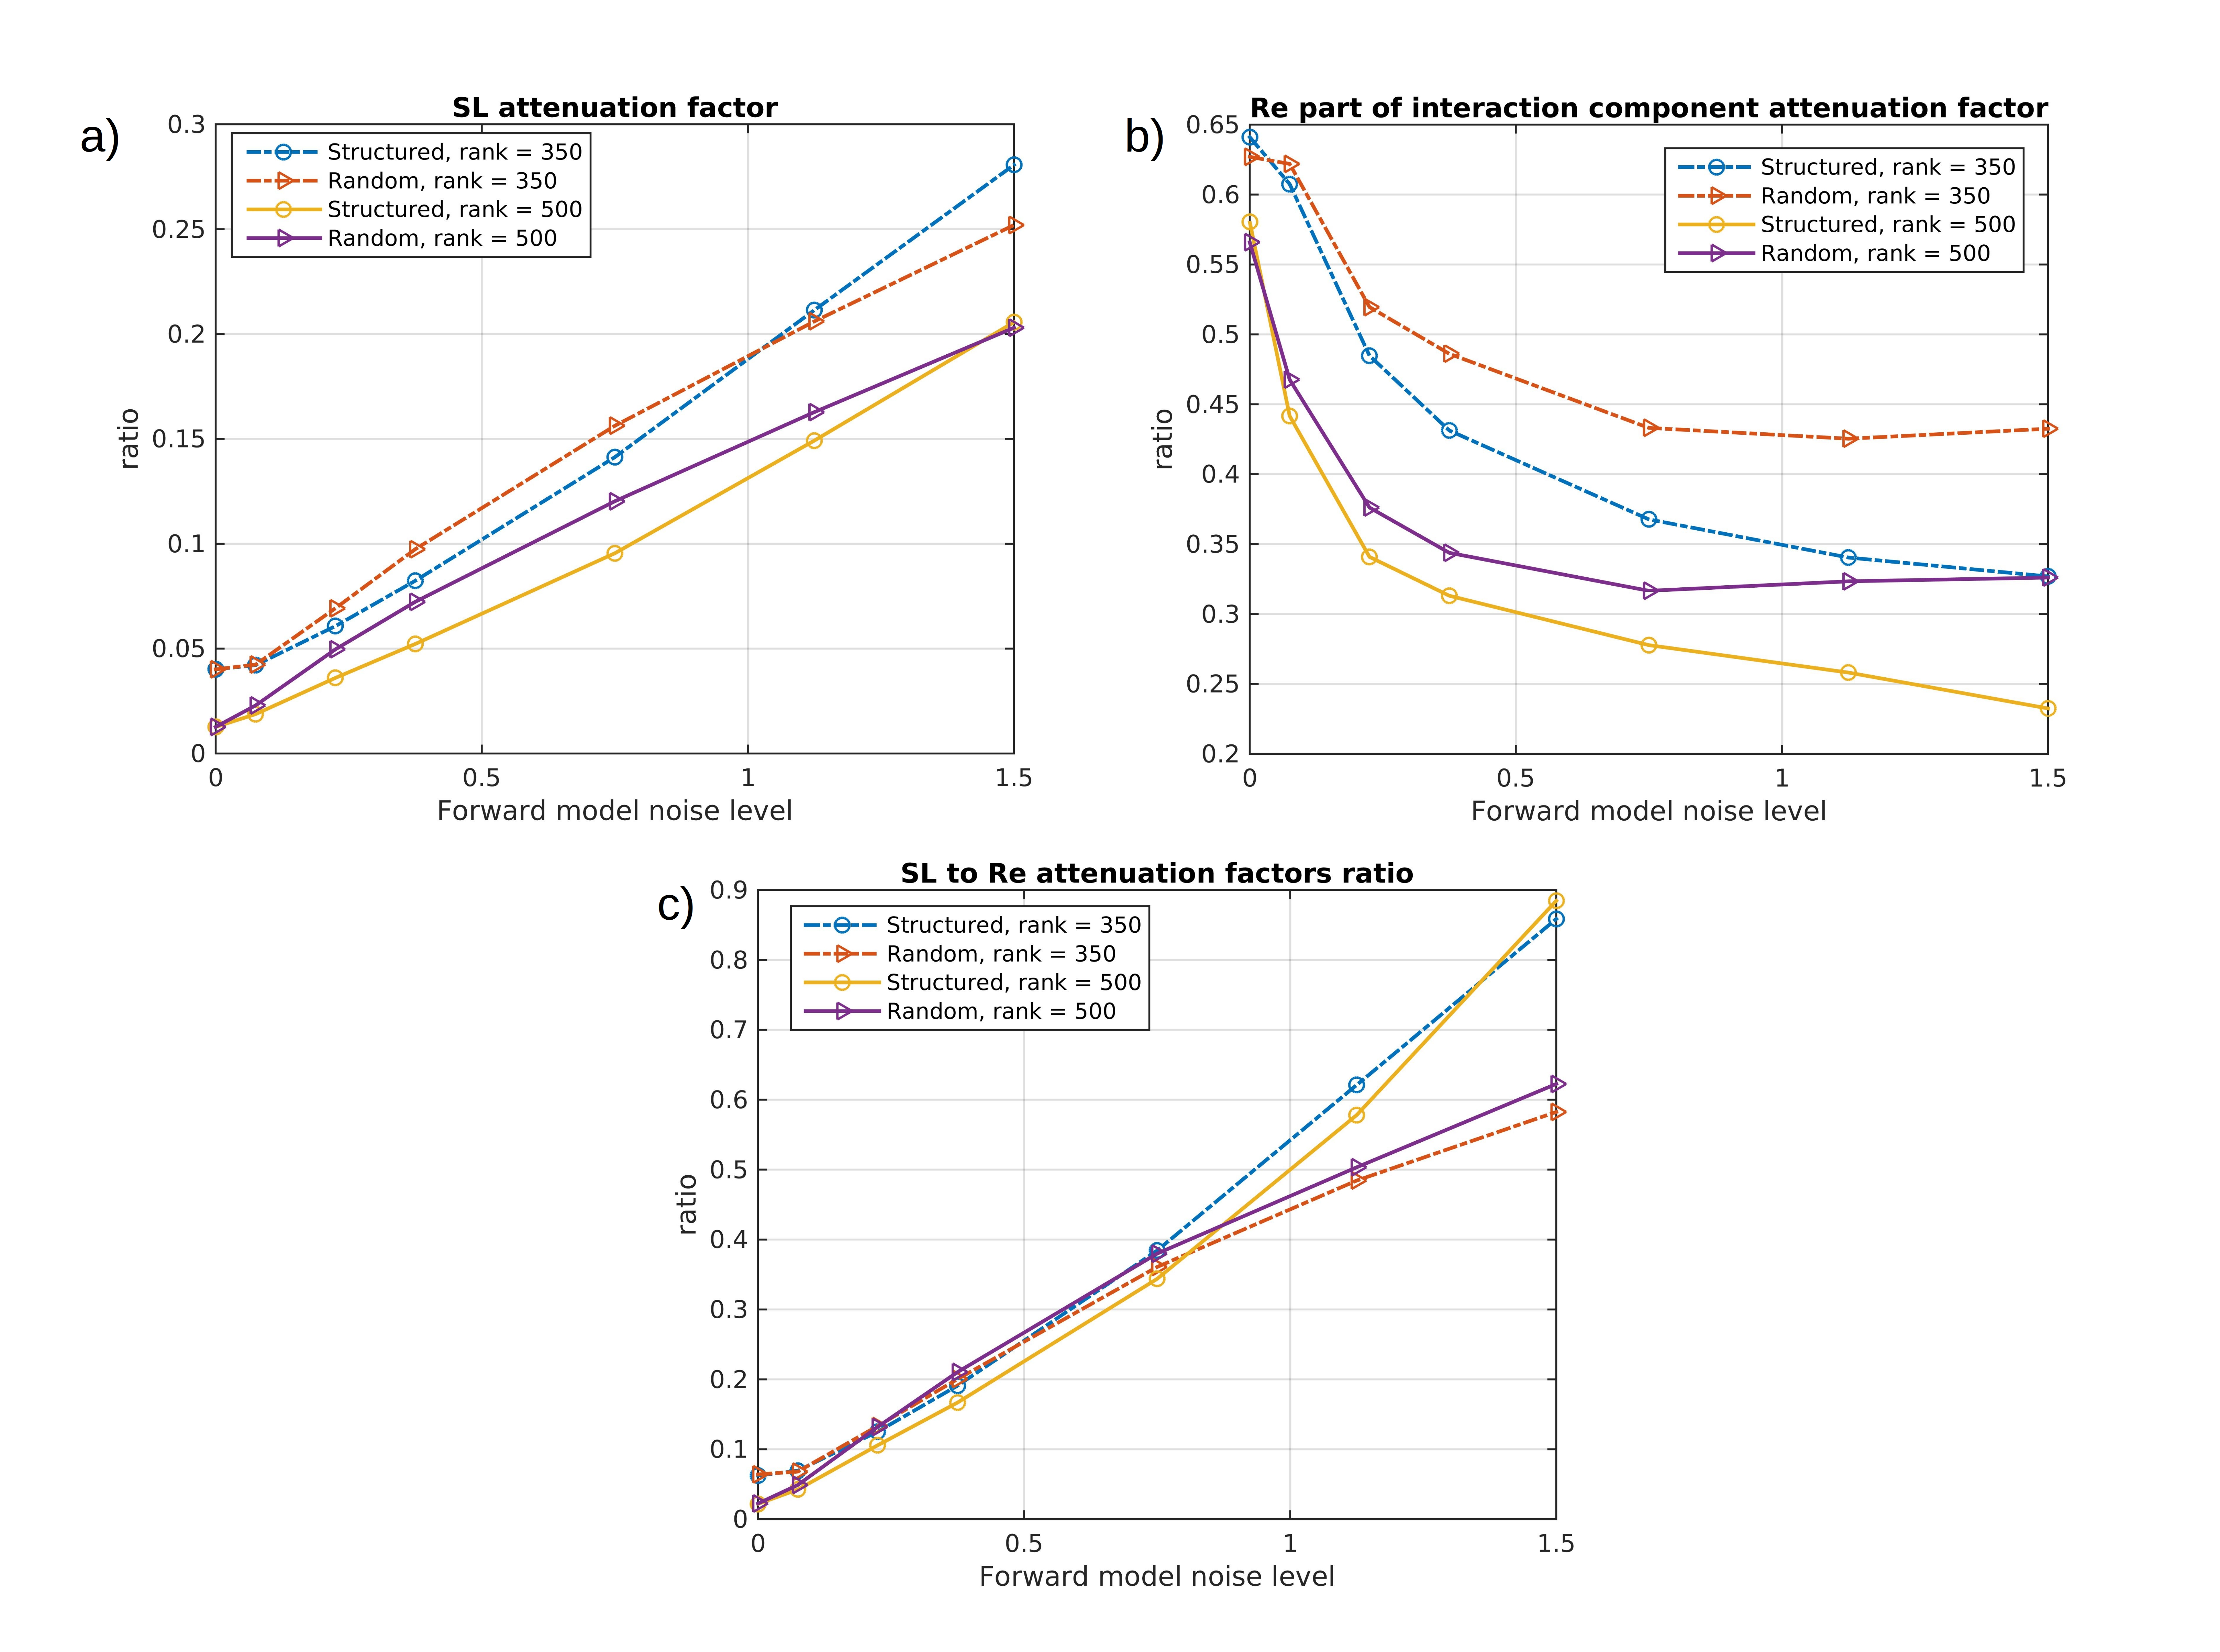
\includegraphics[width=1\textwidth]{../images/psiicos_paper/Figure15_hr.jpg}
\caption{Влияние шума в прямой модели на качество проекции.}\label{fig:15} %Figure 15
  На панели (a) изображена зависимость коэффициента затухания от интенсивности шума $\alpha$.
  Панель (b) показвает коэффициент ослабления мощности в подпространстве $S_{\Re}$.
  На панели (с) нарисовано подавление мощности в подпространстве SL по сравнению с мощностью в $S_{\Re}$.
  Как видим, оно монотонно убывает с ростом интенсивности шума в прямой модели.
 \end{figure}

Из-за пересечения подпространств $S_{SL}$ и $S_{\Re} $ при попытке
подавить компоненту протечки сигнала, алгоритм также подавляет мощность в
подпространстве истинного взаимодействия $S_{\Re}$. Неточности в прямой модели
увеличивают нежелательное подавление мощности в подпространстве $S_{\Re} $ и уменьшают
эффективность подавления мощности в подпространтве протечки сигнала.
Такое ухудшение производительности с увеличением погрешности в прямой модели
можно охарактеризовать соотношением коэффициентов затухания 2-топографий в подпространствах $S_{SL}$ и $S_{\Re}$.
Когда это соотношение меньше единицы, мы можем сказать, что мощность в подпространстве $S_{SL}$
уменьшилась сильнее, чем мощность в подпространстве $ S_{\Re}$. Следовательно
чем меньше это соотношение, тем лучше производительность предлагаемой схемы.

На панели (c) рисунка~\ref{fig:15} мы отобразили соотношение коэффициентов ослабления мощности в подпространствах
$S_{SL}$ и $ S_{\Re}$. Как мы видим, значение этого отношения плавно меняется с
ростом интенсивности шума в прямой модели и остается низким для уровня шума 10 \%.

На основании представленных численных результатов мы можем заключить, что метод
является достаточно надежным для типичных уровней шума в прямой модели и может
использоваться в реальных условиях.  Однако, как и во многих других методах,
использующих прямую модель (например,~\ref{subsec:DICS}), усилия, направленные на
получение более точных прямых моделей способны принести ощутимую отдачу и ими
не следует пренебрегать.



\section{Сравнение стратегий нормализации весов фильтра для метода PSIICOS.}
Как мы уже отмечали в разделе~\ref{subsec:psiicos_normalization_and_spatial_bias},
базовая процедура оценки кросс-спектральных коэффициентов (см.
раздел~\ref{sec:psiicos}) в пространстве источников дает пространственно смещенную оценку.
В разделе~\ref{subsec:psiicos_normalization_and_spatial_bias} мы предложили модификацию
метода, основанную на другой нормализации весов фильтров по аналогии с методом sLORETA,~\cite{Pascual-Marqui2002}.
В этом разделе мы сравнили качество работы базового алгоритма PSIICOS и модифицированного метода
с теоретически пространственно несмещенной оценкой, который мы будем называть PSIICOS Unbiased.

Для сравнения как и ранее мы использовали симуляции Монте-Карло,
описанные в разделе~\ref{sec:monte_carlo_simulation}, со случайно выбираемыми положениями узлов сети
для каждой итерации процедуры. Как и в предыдущих разделах, качество работы алгоритмов мы сравнивали
на основе ROC-кривых и кривых Precition-Reсall. В этом анализе мы ограничились 100 итерациями Монте-Карло.

Результаты этих симуляций для двух значений фазовой задержки (ОСШ=0.2 и ОСШ=1),
а также для трех значений фазового сдвига, $\phi = \pi/20, \phi = \pi/4$ и $\phi=\pi/2 - \pi/20$,
представлены на рис.~\ref{fig:psiicos_vs_unbiased_monte}.

\begin{figure}[htbp]
    \begin{subfigure}[t]{0.5\textwidth}
        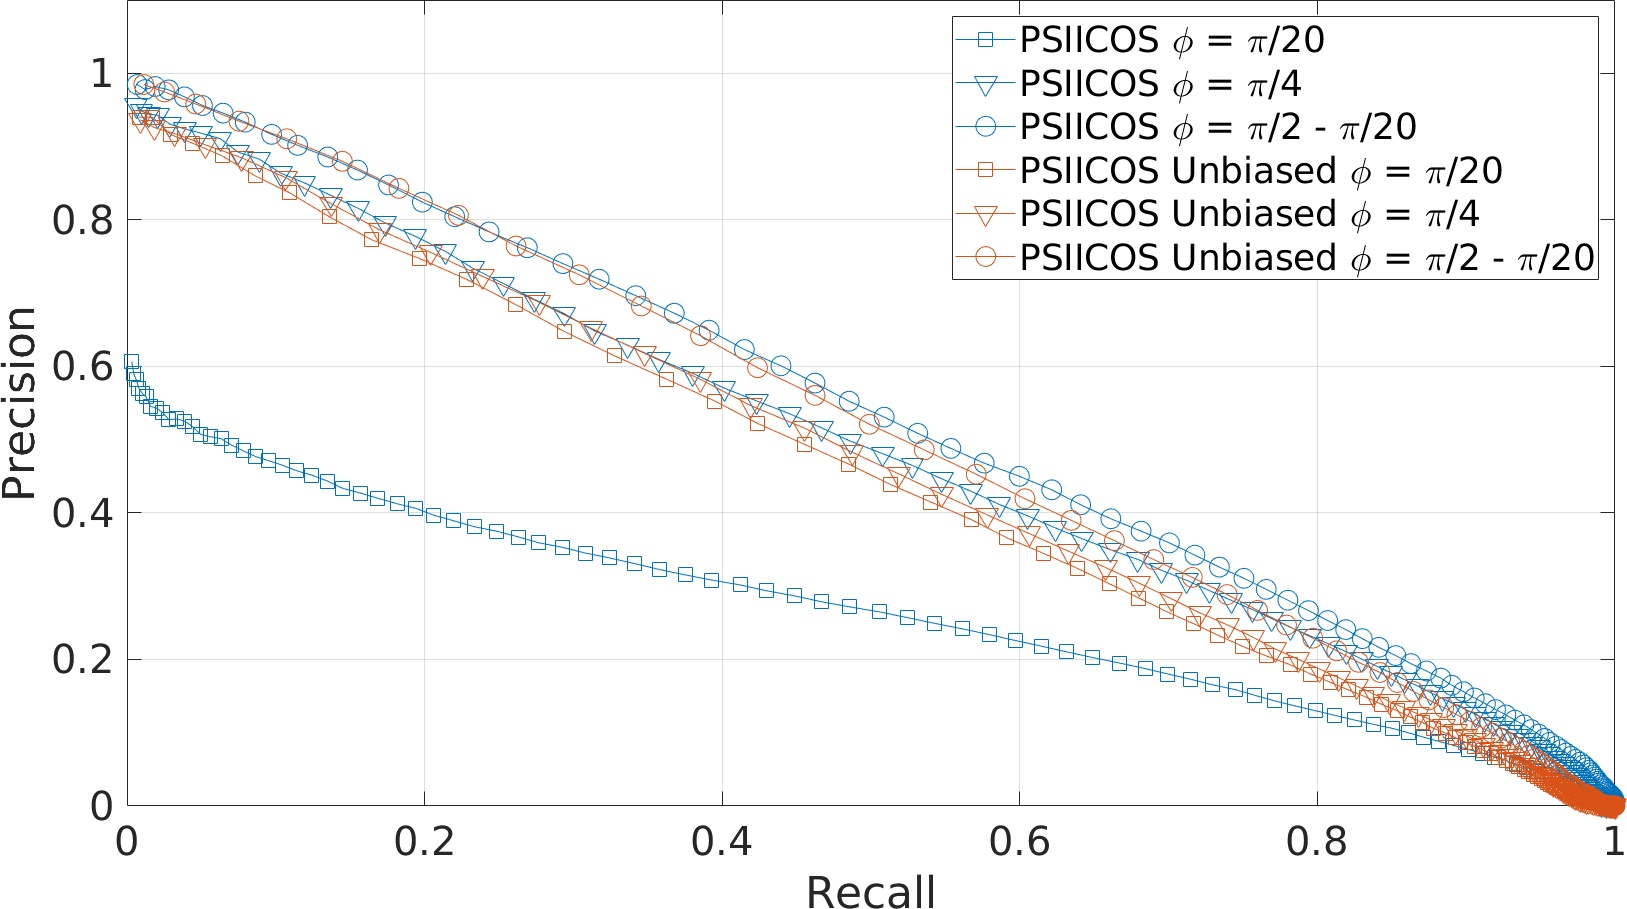
\includegraphics[width=1\textwidth]{../images/pre_rec_snr_1.jpg}
        \caption{Precition-Recall, ОСШ=1}\label{fig:psiicos_vs_unbiased_monte_a}
    \end{subfigure}
        \hspace{-1.5cm}
    \begin{subfigure}[t]{0.5\textwidth}
        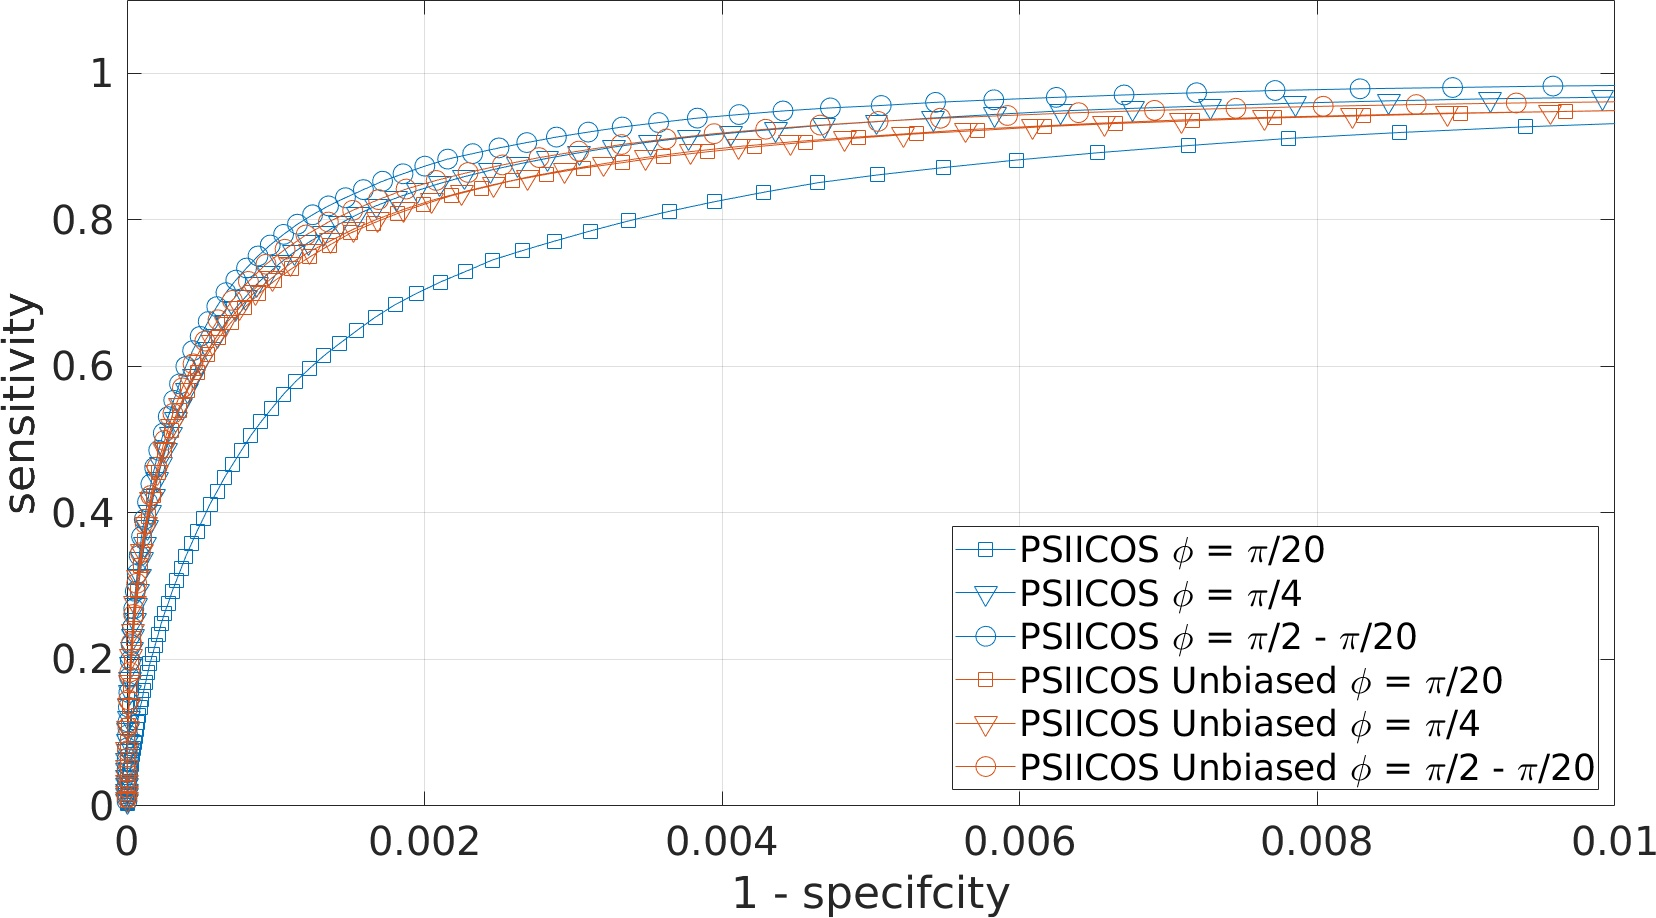
\includegraphics[width=1\textwidth]{../images/roc_snr_1.jpg}
        \caption{ROC, ОСШ=1}\label{fig:psiicos_vs_unbiased_monte_b}
    \end{subfigure}
    \hspace{-2cm}
    \begin{subfigure}[t]{0.5\textwidth}
        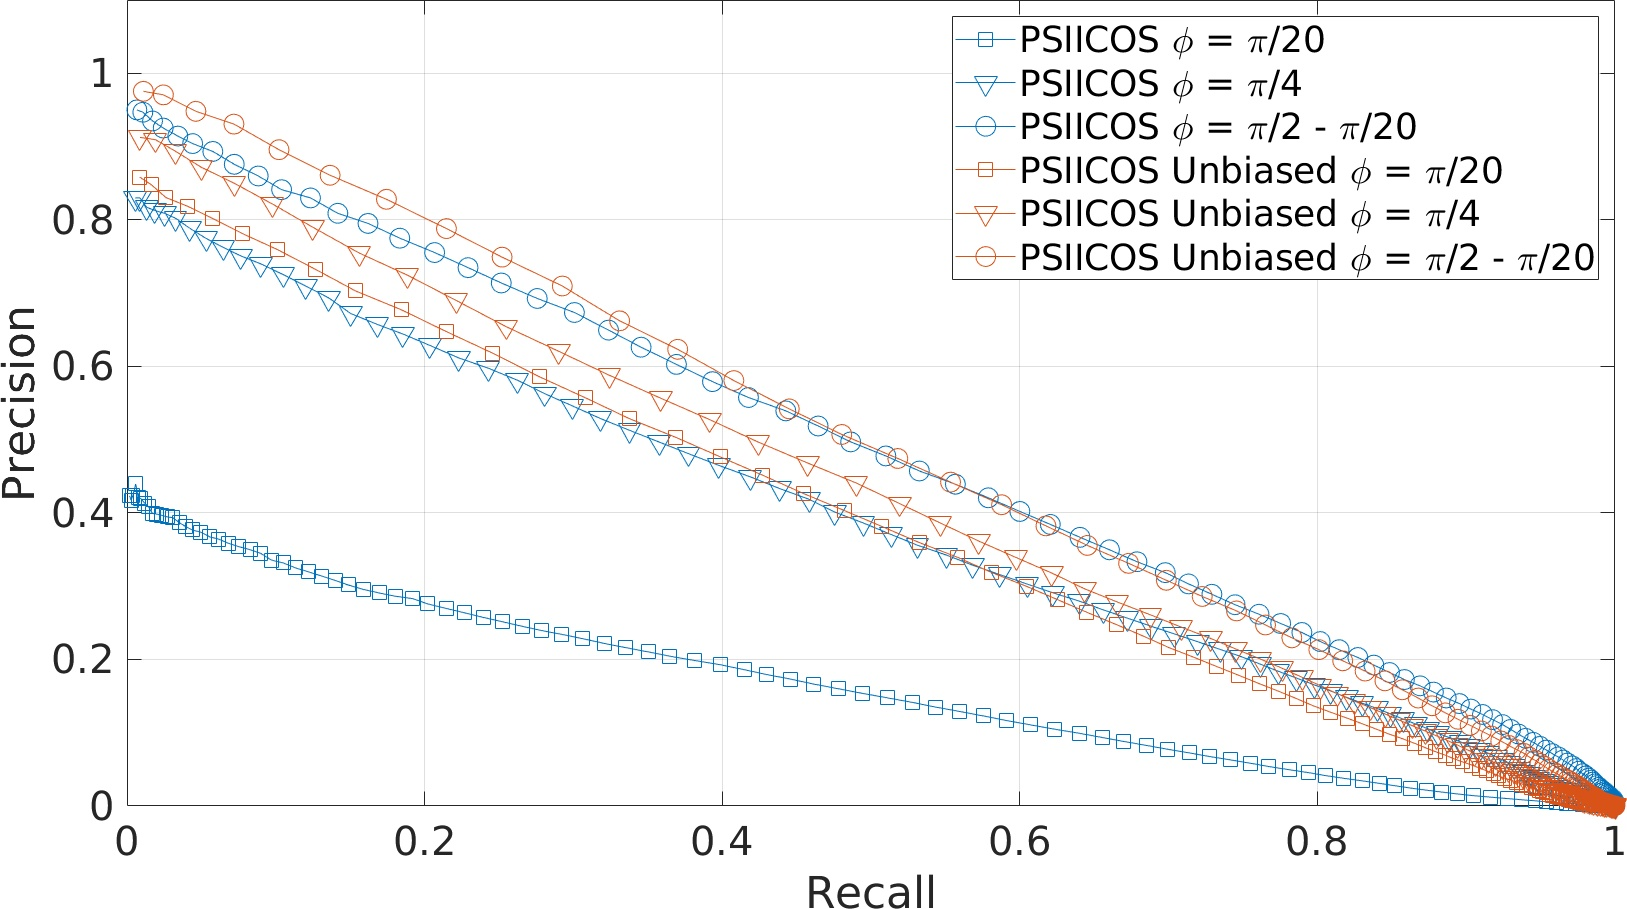
\includegraphics[width=0.99\textwidth]{../images/pre_rec_snr_02.jpg}
        \caption{Precition-Recall, ОСШ=0.2}\label{fig:psiicos_vs_unbiased_monte_c}
    \end{subfigure}
    \begin{subfigure}[t]{0.5\textwidth}
        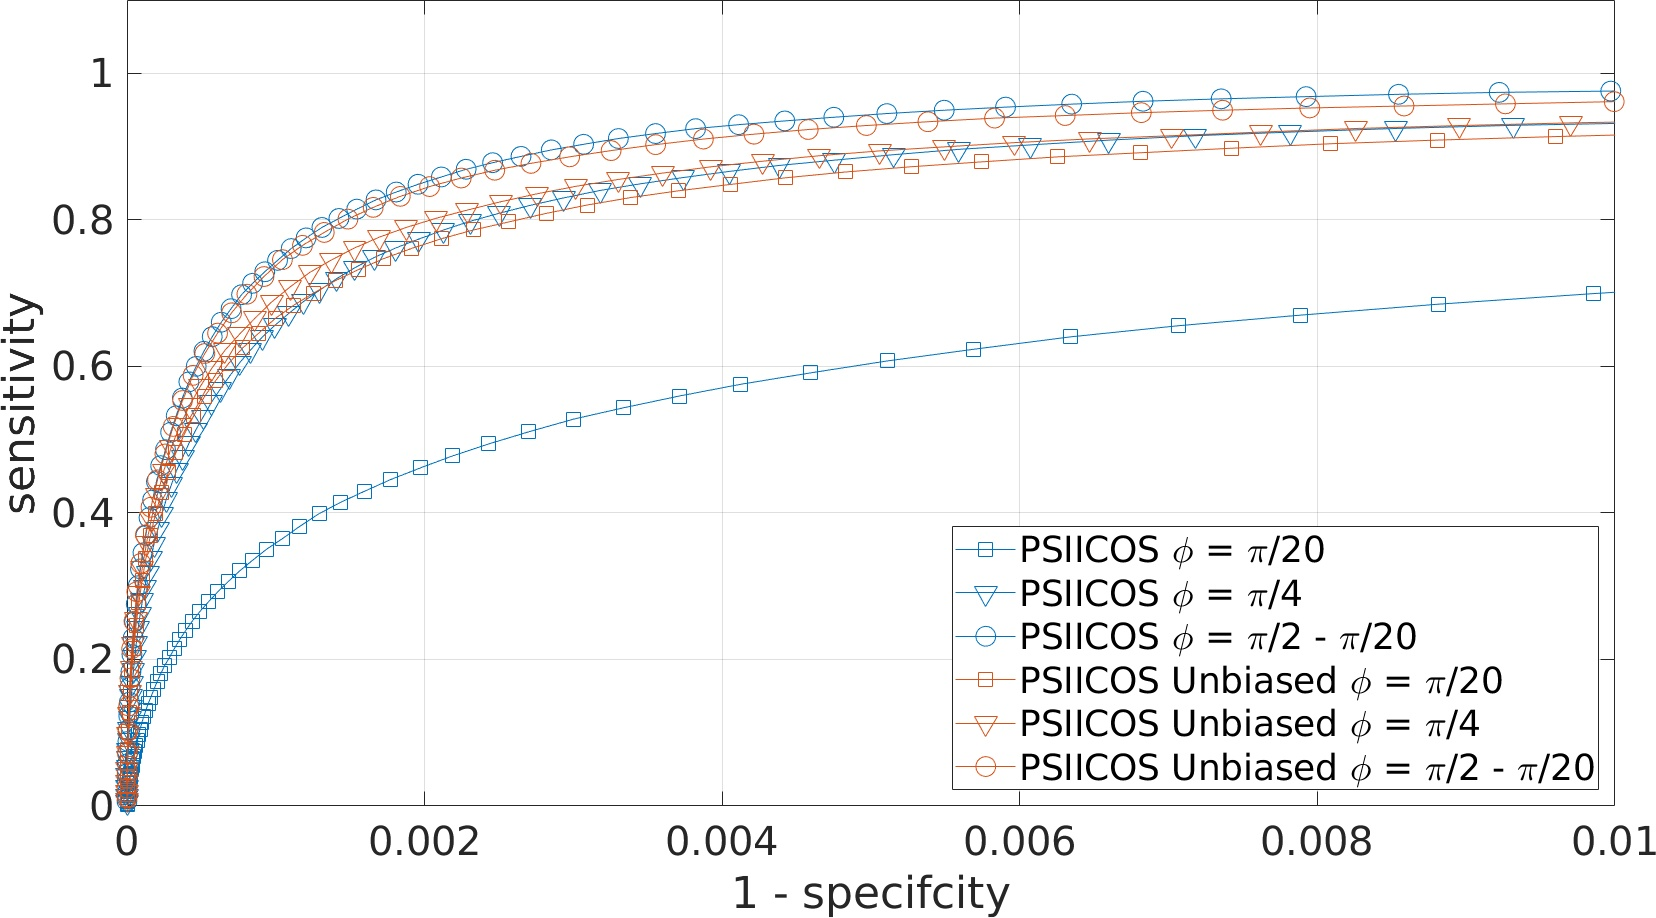
\includegraphics[width=0.99\linewidth]{../images/roc_snr_02.jpg}
        \caption{ROC, ОСШ=0.2}\label{fig:psiicos_vs_unbiased_monte_d}
    \end{subfigure}
    \caption{Сравнение методов PSIICOS и PSIICOS Unbiased в задаче детекции сетей со случайными
    положениями узлов для 100 итераций Монте-Карло.}\label{fig:psiicos_vs_unbiased_monte}
\end{figure}

Из графика~\ref{fig:psiicos_vs_unbiased_monte} видно, что для малых фазовых задержек
как в случае высокого, так и в случае низкого значения ОСШ, метод PSIICOS Unbiased
показывает значительно лучшие результаты. Для остальных значений фазового сдвига
качество решений обеих версий алгоритма приблизительно однаковое с небольшим
преимуществом метода PSIICOS Unbiased для низкого ОСШ.

Такое преимущество PSIICOS Unbiased для $\phi=\pi/20$ объясняется тем, что в методе
PSIICOS при нормализации мы не делали поправку на применение оператора проекции, который
не влияет на 2-топографии мнимой части, но может значительно уменьшать норму 2-топографий
действительной. В этой связи пространственная смещенность оценки методом PSIICOS должна
быть наиболее сильно представлена, когда фазовые задержки сетей близки к нулю, что и вызывает
снижение качества детекции для случая $\phi=\pi/20$.

На рисунке~\ref{fig:psiicos_vs_unbiased_case_3dbrain} представлен характерный пример, взятый с одной из итераций Монте-Карло (ОСШ=1 и $\phi=\pi/20$),
когда алгоритм PSIICOS показал плохие результаты
по сравнению с PSIICOS Unbiased. На графике хорошо виден эффект пространственной смещенности
метода PSIICOS для более глубокого источника в случае низкой фазовой задержки.
Похожая картина наблюдалась и в других отдельно взятых итерациях Монте-Карло, в которых
метод PSIICOS показывал плохое качество решения на индивидуальной кривой Precision-Recall.

\begin{figure}[htbp]
    \begin{subfigure}[t]{0.5\textwidth}
        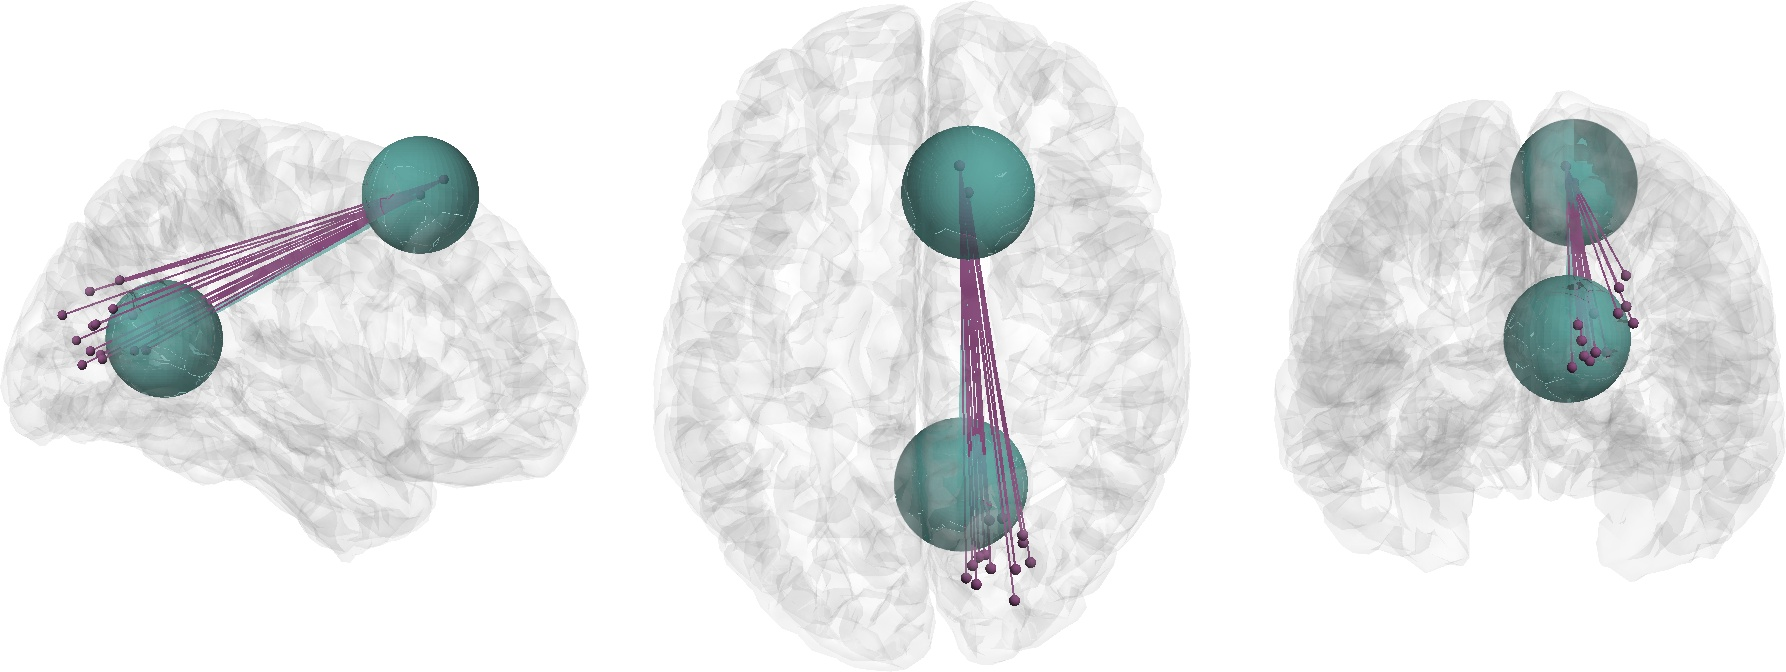
\includegraphics[width=0.99\textwidth]{../images/bias_brain_PSIICOS.jpg}
        \caption{PSIICOS}\label{fig:bias_brain_psiicos}
    \end{subfigure}
    \begin{subfigure}[t]{0.5\textwidth}
        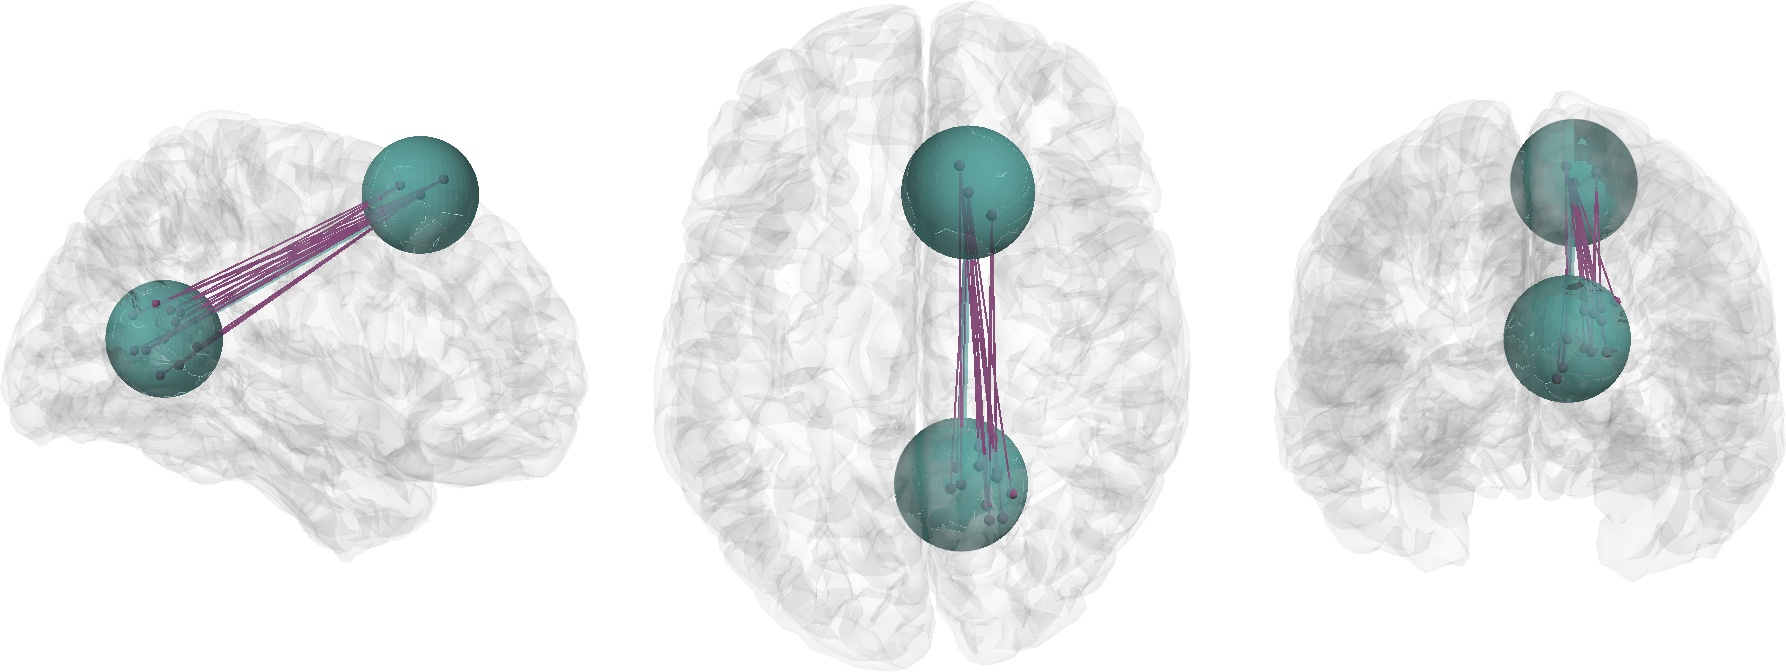
\includegraphics[width=0.99\textwidth]{../images/bias_brain_PSIICOS_Unbiased.jpg}
        \caption{PSIICOS Unbiased}\label{fig:bias_brain_psiicos_unbiased}
    \end{subfigure}
    \caption{Пример плохого решения для алгоритма PSIICOS по сравнению с
        PSIICOS Unbiased в задаче детекции сетей со случайными положениями
        узлов для одной из итераций Монте-Карло и фазового сдвига
        $\phi=\pi/20$.
    }\label{fig:psiicos_vs_unbiased_case_3dbrain}
    Фиолетовые отрезки (по 20 для каждого метода)~--- найденные сети; зелеными
    сферами отмечены зоны, внутри которых найденные сети относились к истинно
    положительным срабатываниям. Радиус каждой сферы равен 1.8 см.
\end{figure}

Далее мы сравнили качество работы двух версий алгоритма PSIICOS в задаче детекции трех
сетей с фиксированными положениями. Пространственная структура и временные профили активации
брались в соответствии с описанием в разделе~\ref{sec:three_ntw}. Как и для сетей со
случайными положениями узлов, мы симулировали сети для двух значений ОСШ и трех
значений фазового сдвига: ОСШ=0.2, ОСШ=1б $\phi=\pi/20, \phi=\pi/4, \phi=\pi/2 - \pi/20$.

Так как в этих симуляциях пространственная структура шума мозга случайна
(она задается как 1000 случайно разбросанных по коре генераторов, см.
раздел~\ref{sec:monte_carlo_simulation}), результаты в разных повторениях
этих симуляций несколько отличаются. Чтобы уменьшить влияние этой случайности,
мы усреднили итоговые кривые по 10 повторениям эксперимента.

\begin{figure}[htbp]
    \begin{subfigure}[t]{0.5\textwidth}
        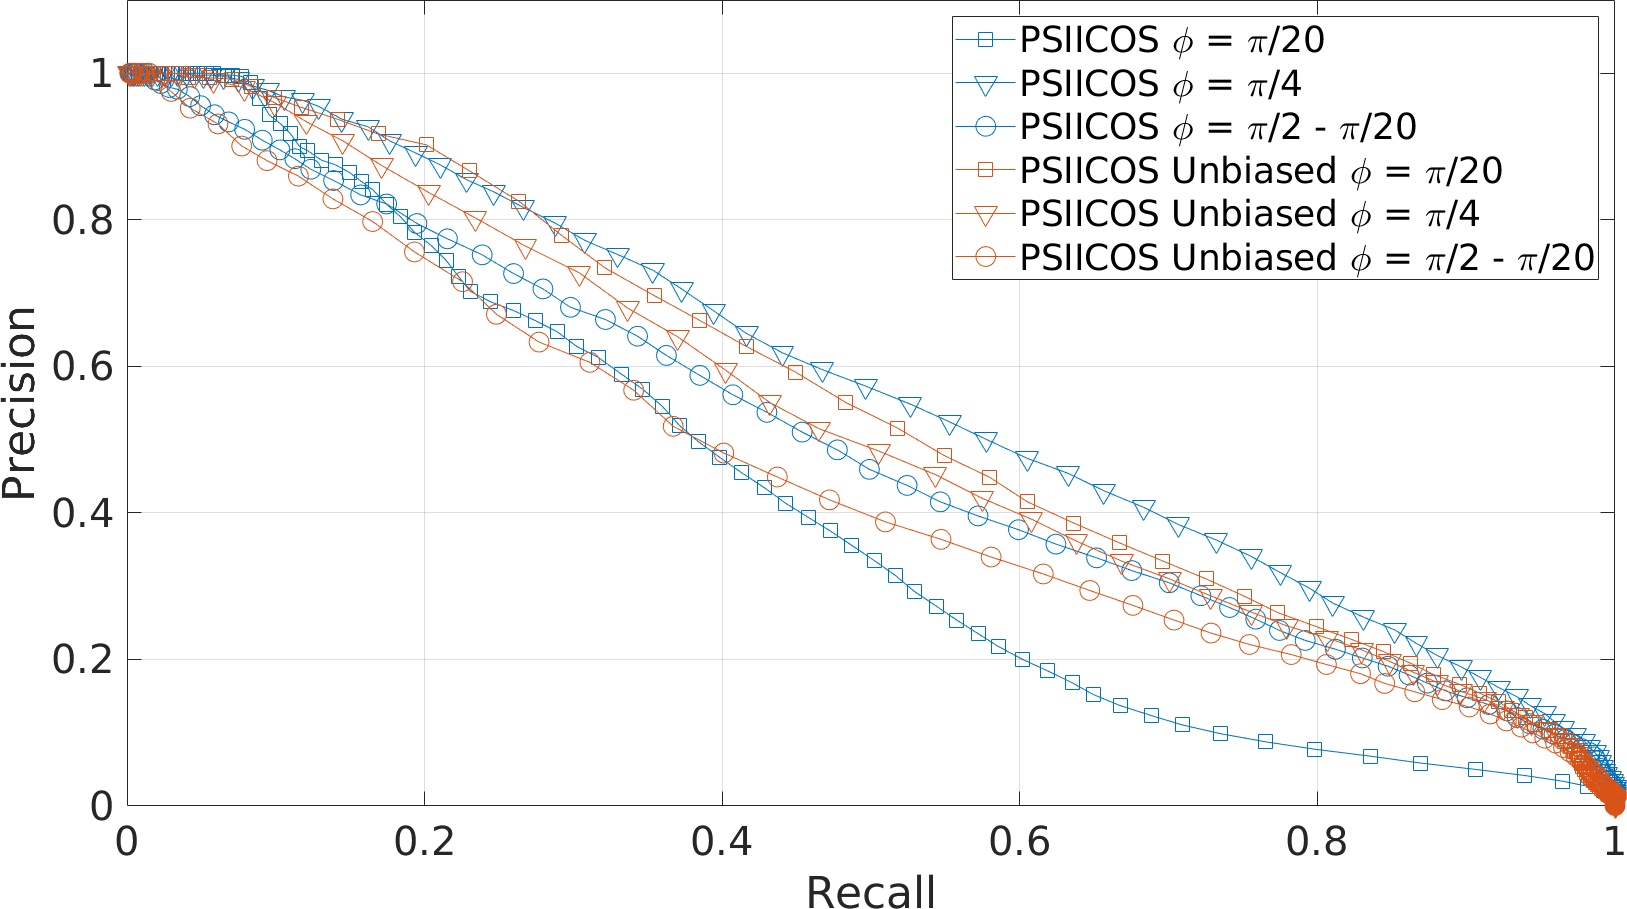
\includegraphics[width=0.99\textwidth]{../images/pre_rec_3_ntw_snr_1.jpg}
        \caption{Precition-Recall, ОСШ=1}\label{fig:psiicos_vs_unbiased_3_ntw_a}
    \end{subfigure}
    \begin{subfigure}[t]{0.5\textwidth}
        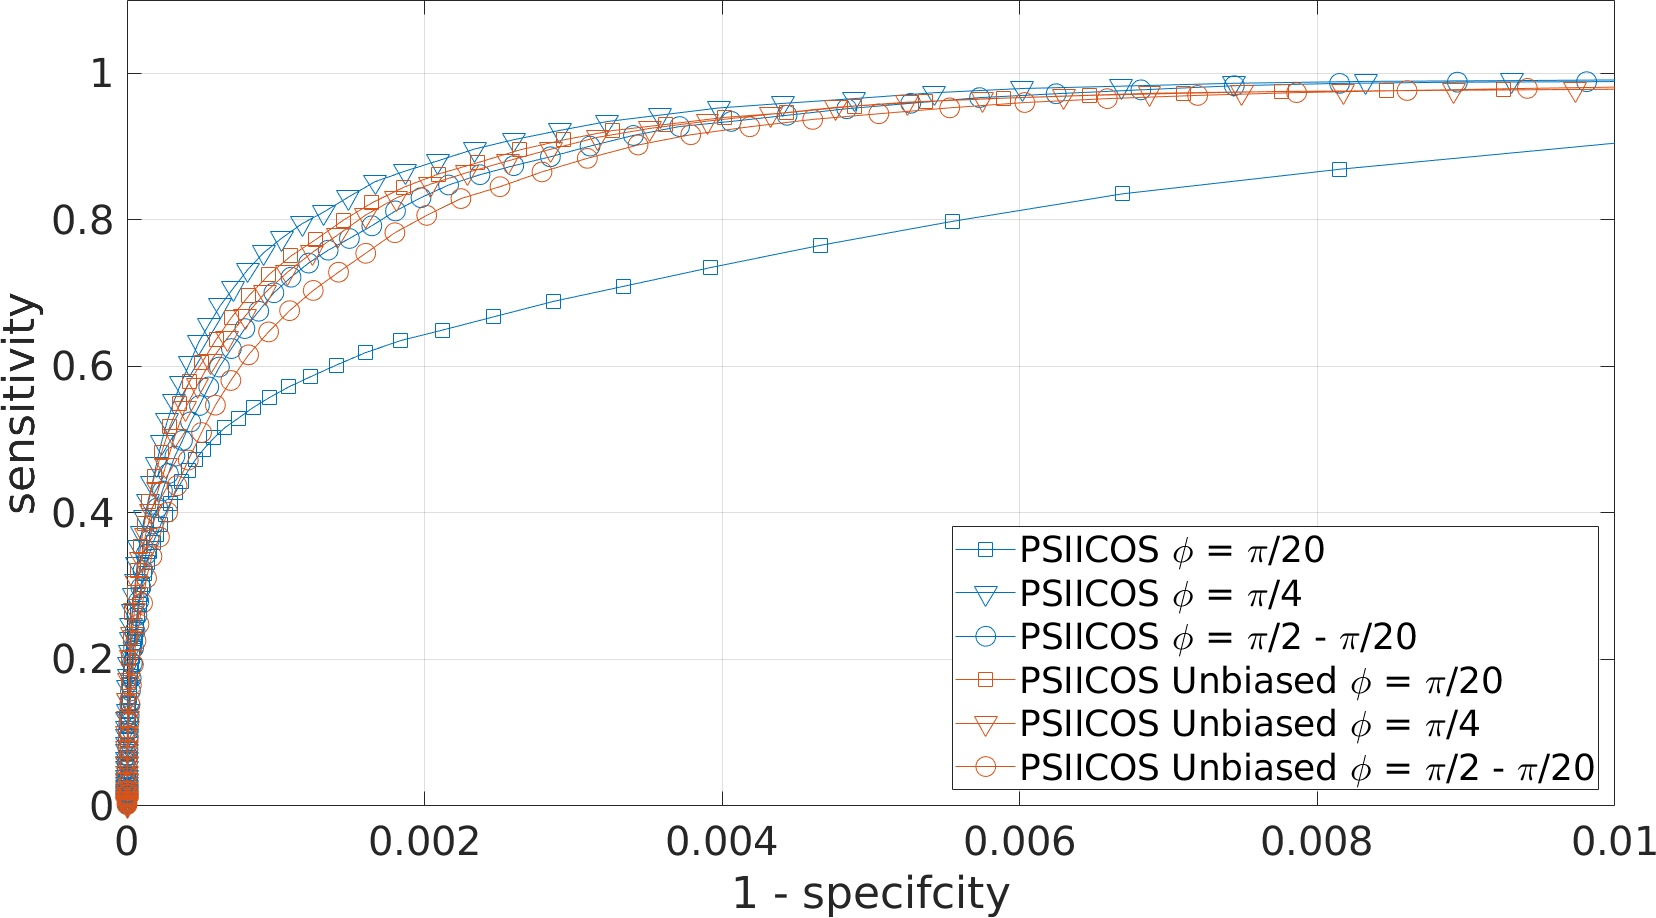
\includegraphics[width=0.99\textwidth]{../images/roc_3_ntw_snr_1.jpg}
        \caption{ROC, ОСШ=1}\label{fig:psiicos_vs_unbiased_3_ntw_b}
    \end{subfigure}
    \begin{subfigure}[t]{0.5\textwidth}
        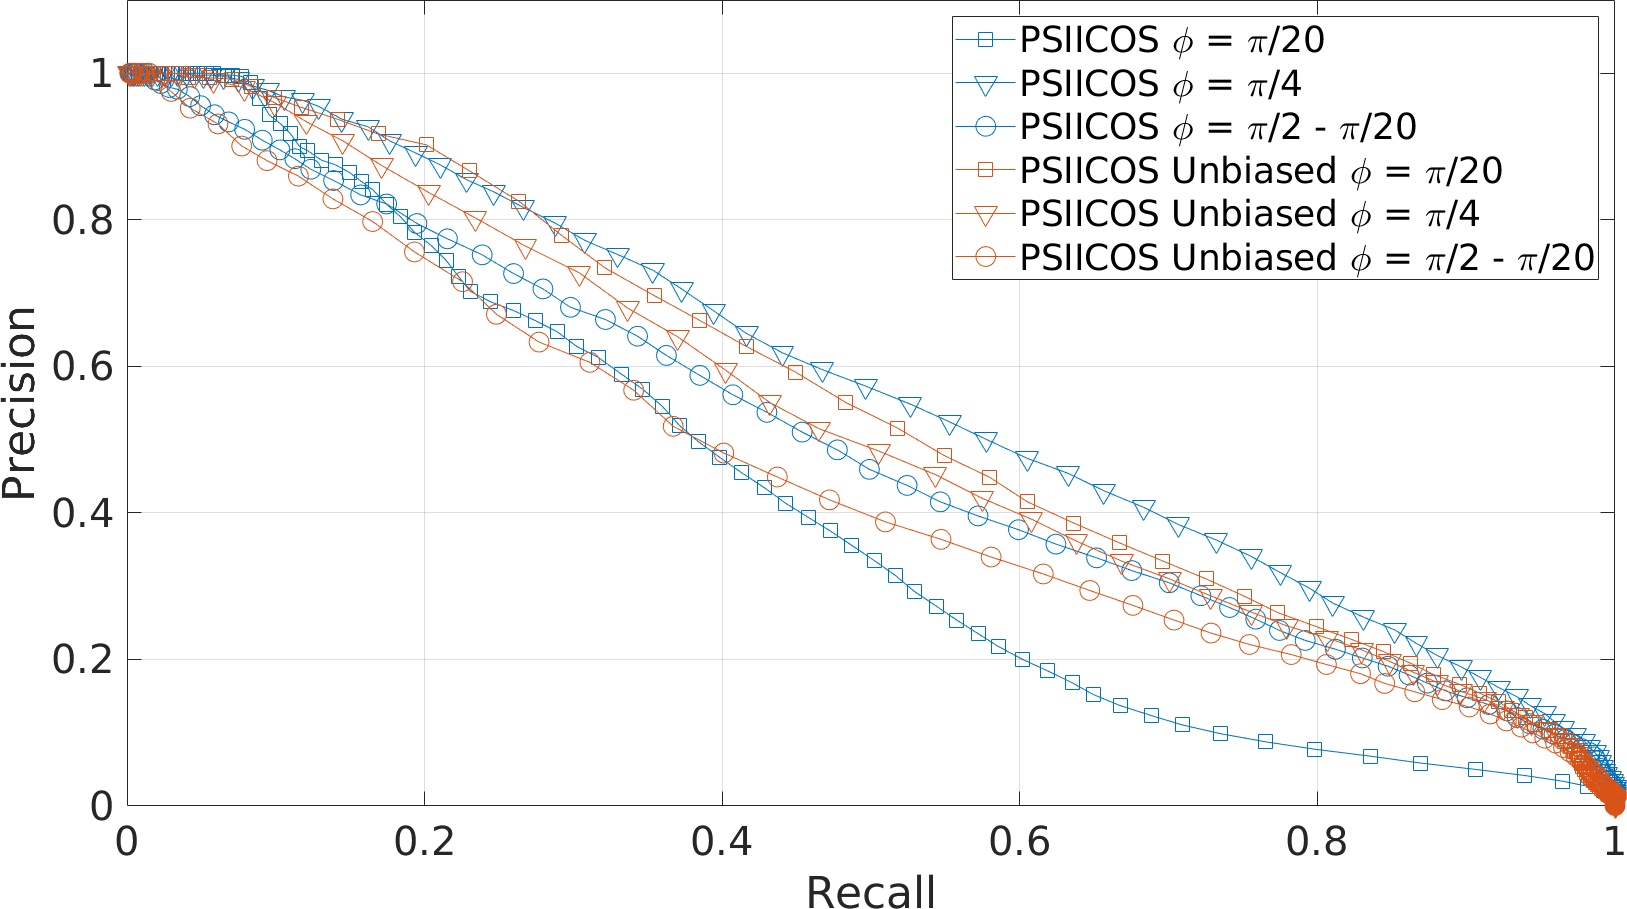
\includegraphics[width=0.99\textwidth]{../images/pre_rec_3_ntw_snr_1.jpg}
        \caption{Precition-Recall, ОСШ=0.2}\label{fig:psiicos_vs_unbiased_3_ntw_c}
    \end{subfigure}
    \begin{subfigure}[t]{0.5\textwidth}
        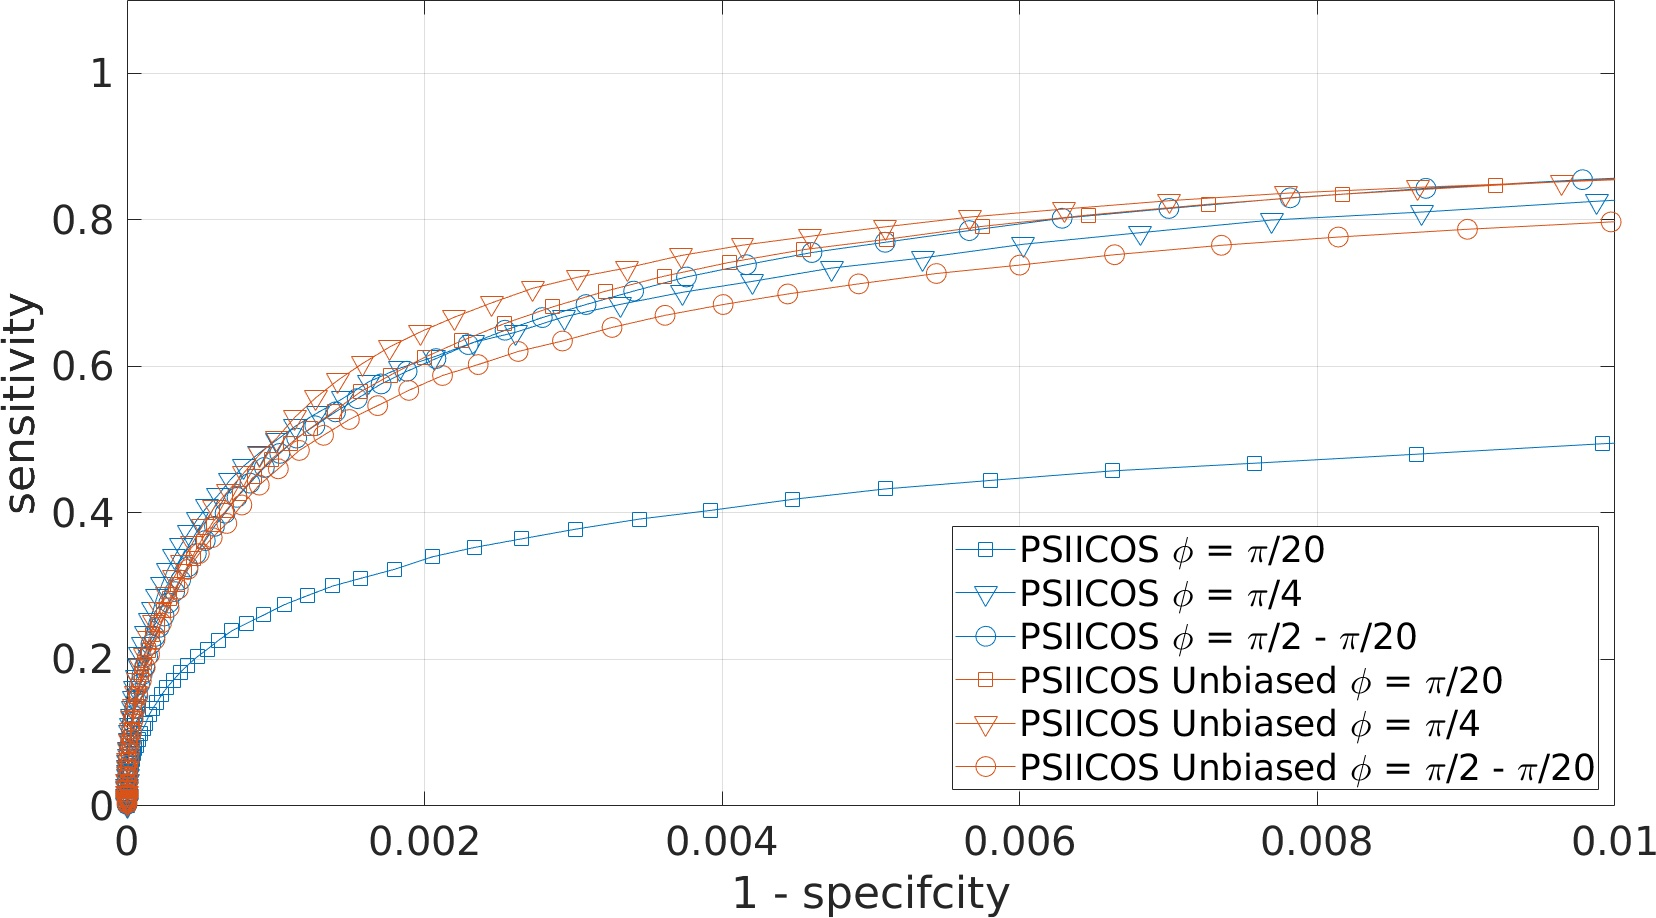
\includegraphics[width=0.99\linewidth]{../images/roc_3_ntw_snr_02.jpg}
        \caption{ROC, ОСШ=0.2}\label{fig:psiicos_vs_unbiased_3_ntw_d}
    \end{subfigure}
    \caption{Сравнение методов PSIICOS и PSIICOS Unbiased в задаче детекции трех сетей
        с фиксированными положениями источников и перекрывающимися временными профилями активации,
        усредненные по 10 повторениям.}\label{fig:psiicos_vs_unbiased_3_ntw}
\end{figure}

Результаты представлены на рис.~\ref{fig:psiicos_vs_unbiased_3_ntw}. Из этих графиков мы
вновь видим, что качество решений метода PSIICOS для малых фазовых задержек несколько проседает
по сравнению с PSIICOS Unbiased. При этом для фазовых сдвигов $\phi=\pi/4, \phi=\pi/2 - \pi/20$
качество решений PSIICOS по кривым оказывается несколько лучше, чем таковое для PSIICOS Unbiased.
Это объясняется способом построения соответствующих кривых и пространственной структурой сетей: метод
PSIICOS Unbiased для этой конкретной конфигурации склонен накапливать больше сетей вокруг одной из истинных
локаций, прежде чем переходить к остальным. Это приводит к выходу пучка отрезков за пределы
сферы, в которую должно попасть решение, что с точки зрения нашей процедуры является ложным срабатыванием,
но для реальных приложений не критично.

\section{Численное исследование метода нормализации кросс-спектральных коэффициентов в пространстве источников (PSIICOS Normalized).}\label{sec:psiicos_normalized_simulations}

В разделе~\ref{subsec:psiicos_normalized} мы обозначили проблему локализации методом PSIICOS,
которая заключается в том, что элементы кросс-спектра зависят не только от фазовой связности
источников, но и от их амплитуд, что не позволяет сделать однозначного вывода о наличии коннективности между парой источников.


\begin{figure}[htbp]
    \begin{subfigure}[t]{0.24\textwidth}
        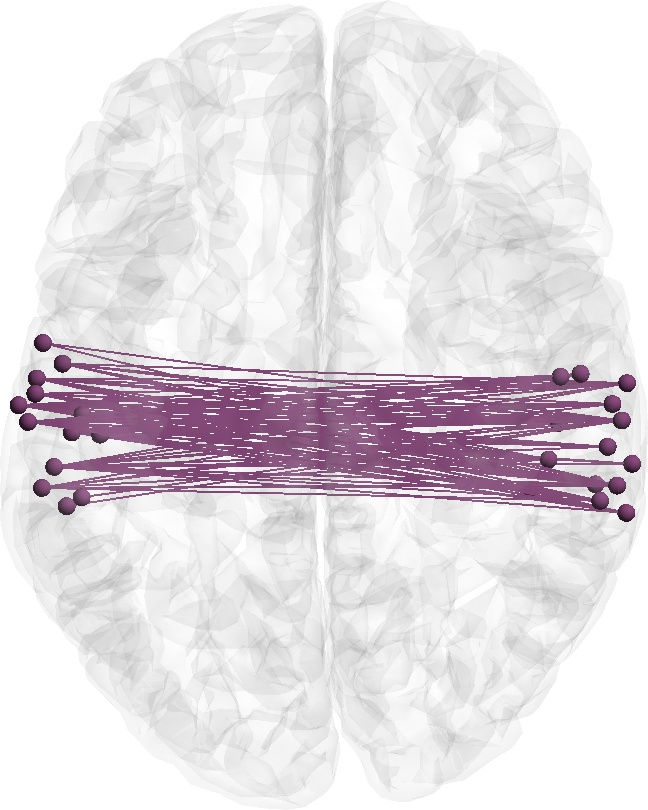
\includegraphics[width=0.99\textwidth]{../images/loreta_brain_jitter_01_snr_02_phase_lag_07854.jpg}
        \caption{$\alpha=0.1$, ОСШ=0.2}\label{fig:unbiased_1_ntw_a}
    \end{subfigure}
    \begin{subfigure}[t]{0.24\textwidth}
        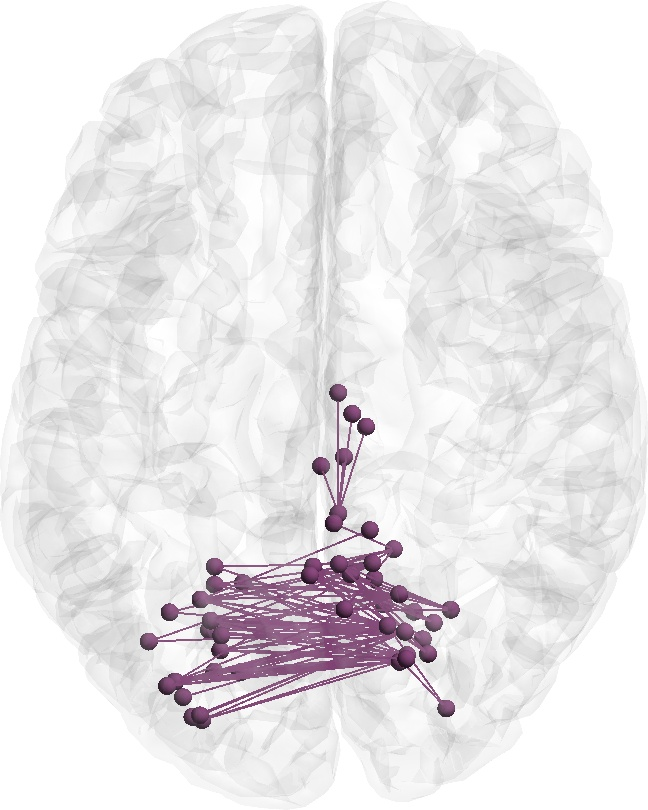
\includegraphics[width=0.99\linewidth]{../images/loreta_brain_jitter_2_snr_02_phase_lag_07854.jpg}
        \caption{$\alpha=2$, ОСШ=0.2}\label{fig:unbiased_1_ntw_b}
    \end{subfigure}
    \begin{subfigure}[t]{0.24\textwidth}
        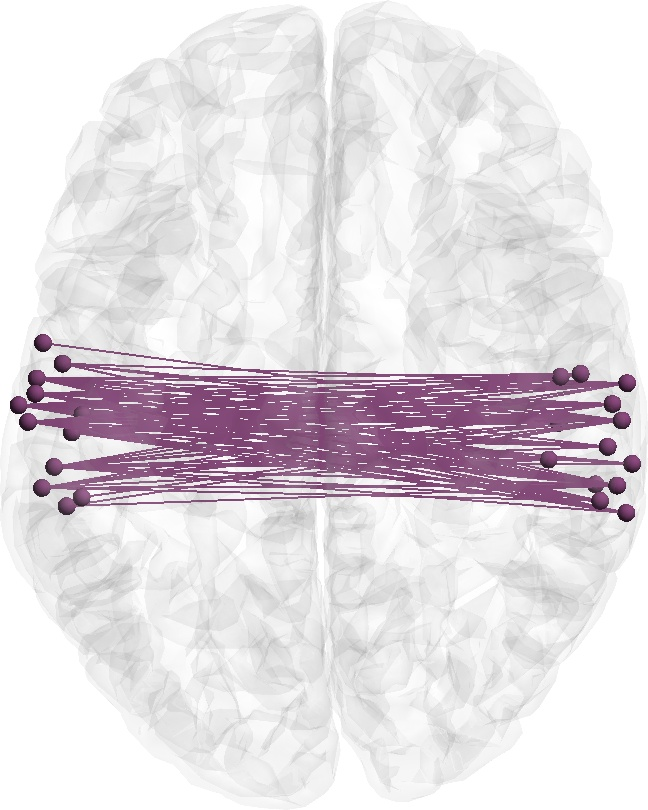
\includegraphics[width=0.99\textwidth]{../images/loreta_brain_jitter_01_snr_1_phase_lag_07854.jpg}
        \caption{$\alpha=0.1$, ОСШ=1}\label{fig:unbiased_1_ntw_c}
    \end{subfigure}
    \begin{subfigure}[t]{0.24\textwidth}
        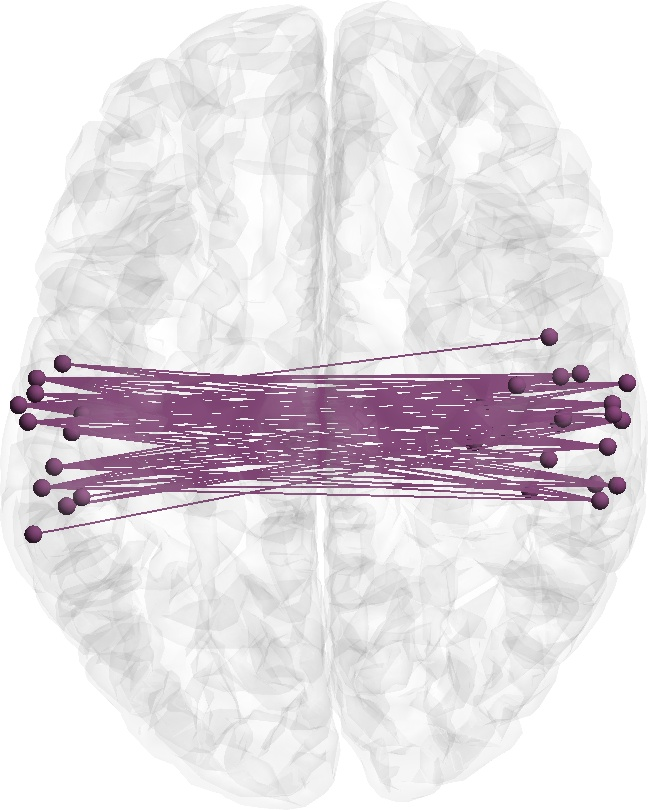
\includegraphics[width=0.99\linewidth]{../images/loreta_brain_jitter_2_snr_1_phase_lag_07854.jpg}
        \caption{$\alpha=2$, ОСШ=1}\label{fig:unbiased_1_ntw_d}
    \end{subfigure}
    \caption{Локализация сети с фиксированными положениями узлов методом PSIICOS Unbiased для 
    фазового сдвига $\phi=\pi/4$ для высокого и низкого ОСШ (0.2 и 1) в
    случае сильной связности ($\alpha=0.1$) и отсутствия связности ($\alpha=2$)}\label{fig:unbiased_breaks_in_high_snr}
\end{figure}

На рис.~\ref{fig:unbiased_breaks_in_high_snr} мы проиллюстрировали этот эффект.
Для построения этого графика мы использовали симуляции, аналогичные описанным в
разделе~\ref{sec:three_ntw}, но на этот раз мы ограничились только одной
центральной сетью. На рис.~\ref{fig:unbiased_breaks_in_high_snr} мы изобразили
100 самых мощных сетей, полученных алгоритмом PSIICOS Unbiased для низкого и
высокого значения ОСШ при низком и высоком значении разброса фазы сети, $\alpha$.
Параметр $\alpha$ при симуляциях регулировал величину случайной добавки к постоянной
разности фаз для каждой сети. Чем ближе к нулю значение $\alpha$, тем сильнее
фазовая связность. Значение $\alpha=2$ соответствует полному отсутствию связности.

Из рис.~\ref{fig:unbiased_breaks_in_high_snr} видно, что алгоритм корректно находит
сети в случае высокой фазовой связности ($\alpha=0.1$, панели~\ref{fig:unbiased_1_ntw_a},~\ref{fig:unbiased_1_ntw_c}), однако при отсутствии фазовой связности ситуация не столь хороша.
В этом случае при низком ОСШ (панель~\ref{fig:unbiased_1_ntw_b}) алгоритм находит
шумовые сети, но так как выдаваемые им значения для сетей ненормированные, мы не можем
отбросить эти сети по одному прогону алгоритма. Тем не менее, эту проблему можно
решить, используя процедуру бутстрэпа и считая индекс воспроизводимости: для шумовых сетей
он будет низким, а для настоящих~--- высоким.

Хуже обстоит дело в случае отсутствия фазовой связности и высокого значения ОСШ (панель~\ref{fig:unbiased_1_ntw_d}). В при таких параметрах алгоритм находит ошибочно находит центральную сеть
из-за того, что мощность ее узлов выделяется на фоне окружающего шума, а также из-за
коррелированности их временных профилей активации. В этом случае процедура бутстрапа
покажет воспроизводимую сеть, хотя в действительности фазовой связности нет.

В разделе~\ref{subsec:psiicos_normalized} мы предложили
модификацию метода PSIICOS, которая осуществляет нормализацию кросс-спектральных
коэффициентов с учетом наличия протечки сигнала. За счет нормализации мы можем справиться
с ложноположительными срабатываниями, аналогичными случаю~\ref{fig:unbiased_1_ntw_d}.

\begin{figure}[htbp]
    \begin{subfigure}[t]{0.5\textwidth}
        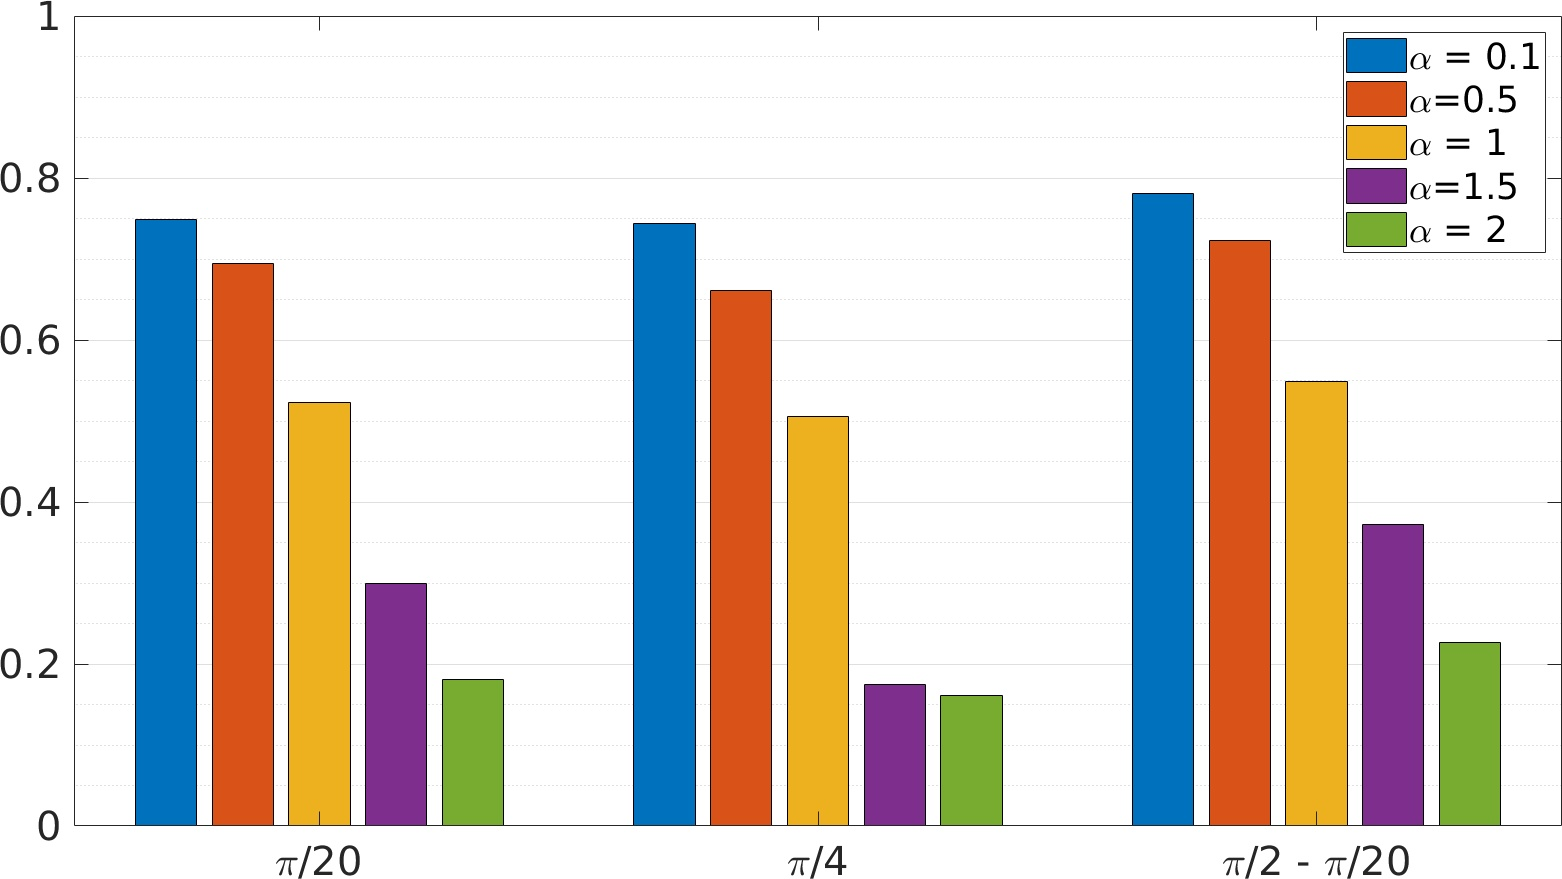
\includegraphics[width=0.99\textwidth]{../images/bars_snr_02.jpg}
        \caption{ОСШ=0.2}\label{fig:bars_a}
    \end{subfigure}
    \begin{subfigure}[t]{0.5\textwidth}
        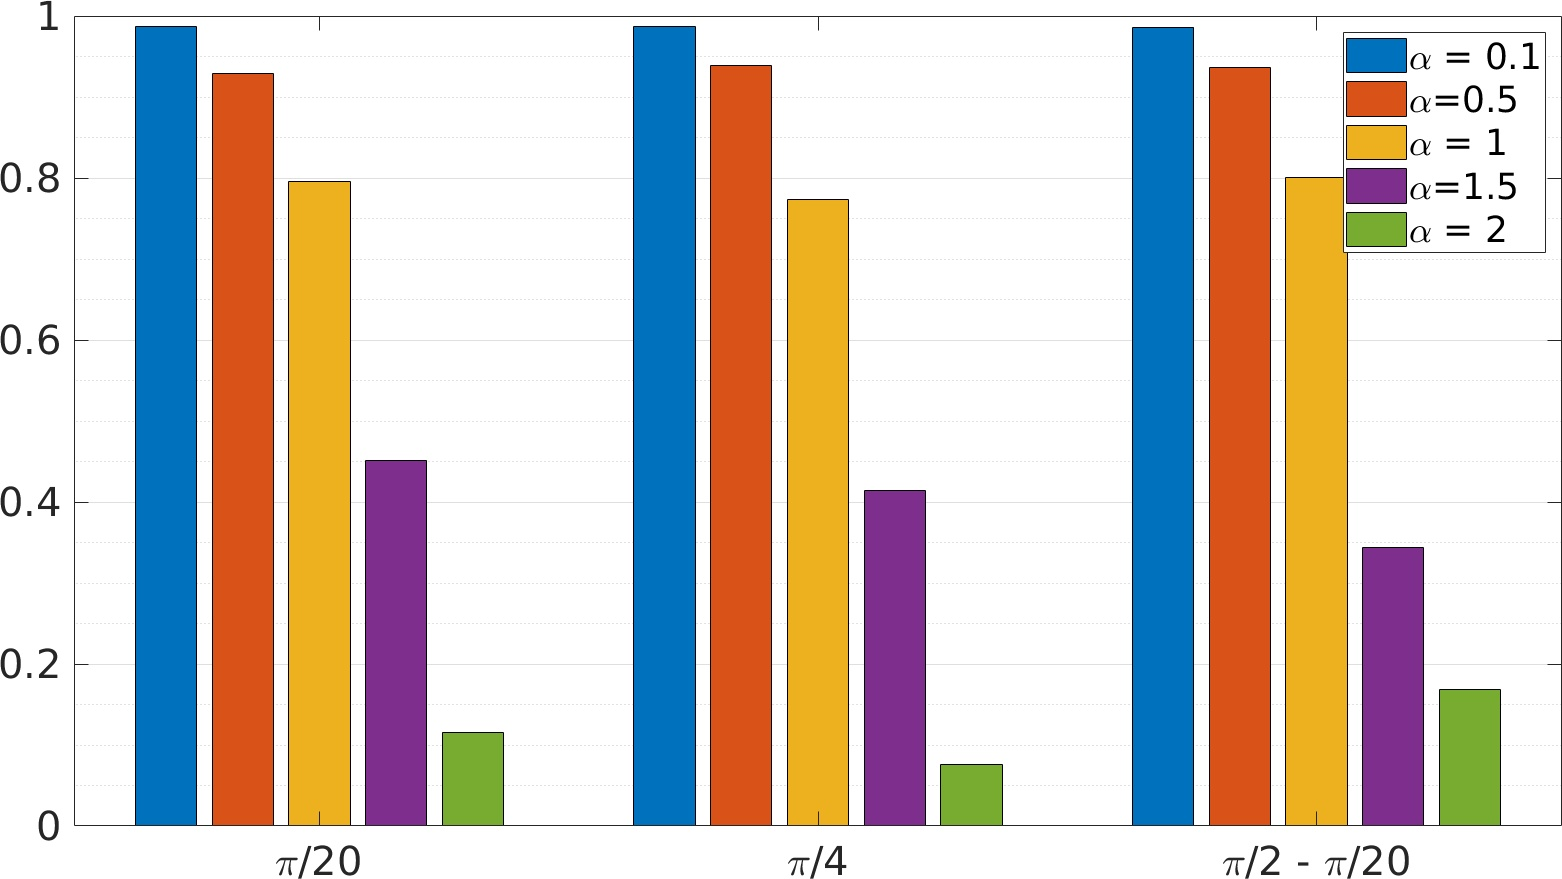
\includegraphics[width=0.99\linewidth]{../images/bars_snr_1.jpg}
        \caption{ОСШ=1}\label{fig:bars_b}
    \end{subfigure}
    \caption{Нормализованный индекс фазовой связности, полученный методом
    PSIICOS Normalized для одной симулированной сети в условиях высокого и низкого ОСШ
    в зависимости от индекса истинной фазовой связности $\alpha$ и значения
    фазовой задержки.}\label{fig:bars_normalized_index}
\end{figure}

Чтобы продемонстрировать это, мы симулировали данные для одной центральной сети
для набора индексов фазовой связности в диапазоне от 0.1 (сильная связность) до
2 (связность отсутствует) для низкого и высокого значения ОСШ (0.2 и 1 соответственно)
и для трех значений фазовых сдвигов ($\phi=\pi/20, \phi = \pi/4, \phi=\pi/2 - \pi/20$).
Для каждой комбинации параметров мы применяли метод PSIICOS Unbiased и отбирали
сети с максимальным абсолютным значением оцененного элемента кросс-спектра.
Для этой сети мы проводили нормализацию в соответствии с процедурой, описанной
в разд.~\ref{subsec:psiicos_normalized} и рисовали полученное значение на графике.
Результаты представлены на рис.~\ref{fig:bars_normalized_index}.

Из этого графика видно, что в случае, когда фазовая связность отсутствует
($\alpha=2$), полученные нормализованные значения не превосходят порога в 0.3.
При этом нормализованный индекс монотонно убывает с ростом параметра $\alpha$.

Вместе с тем отметим, что более высокое значение ОСШ позволяет получать более
высокие значения для нормализованного индекса для одинаковых значений $\alpha$
в случае, когда фазовая связность есть, оставляя индекс на том же уровне или
ниже, когда ее нет. Похожий эффект ослабления значений меры коннективности при
понижении ОСШ отмечали авторы метода wPLI,~\cite{wPLI}.

Индекс, полученный методом PSIICOS Normalized, теоретически может быть
использован и для локализации сетей, однако такая нормировка приводит к
появлениию пространственной смещенности оценки (рассуждения аналогичны изложенным
в разд.~\ref{subsec:psiicos_normalization_and_spatial_bias}), поэтому для
использования на практике разумнее сначала локализовать потенциальные сети
одним из методов (PSIICOS Unbiased или GO-PSIICOS) и затем использовать
PSIICOS Normalized для удаления ложноположительных срабатываний из-за мощности.

\section{Демонстрация работы метода GO-PSIICOS на симуляционных данных.}

В этом разделе мы продемонстрировали работу метода GO-PSIICOS, который решает
задачу поиска сетей методом глобальной оптимизации и обладает свойством разреженности
решений по пространству, что позволяет подавить ``призрачные взаимодействия'' в
решении.


\begin{figure}[htbp]
    \begin{subfigure}[t]{0.6\textwidth}
        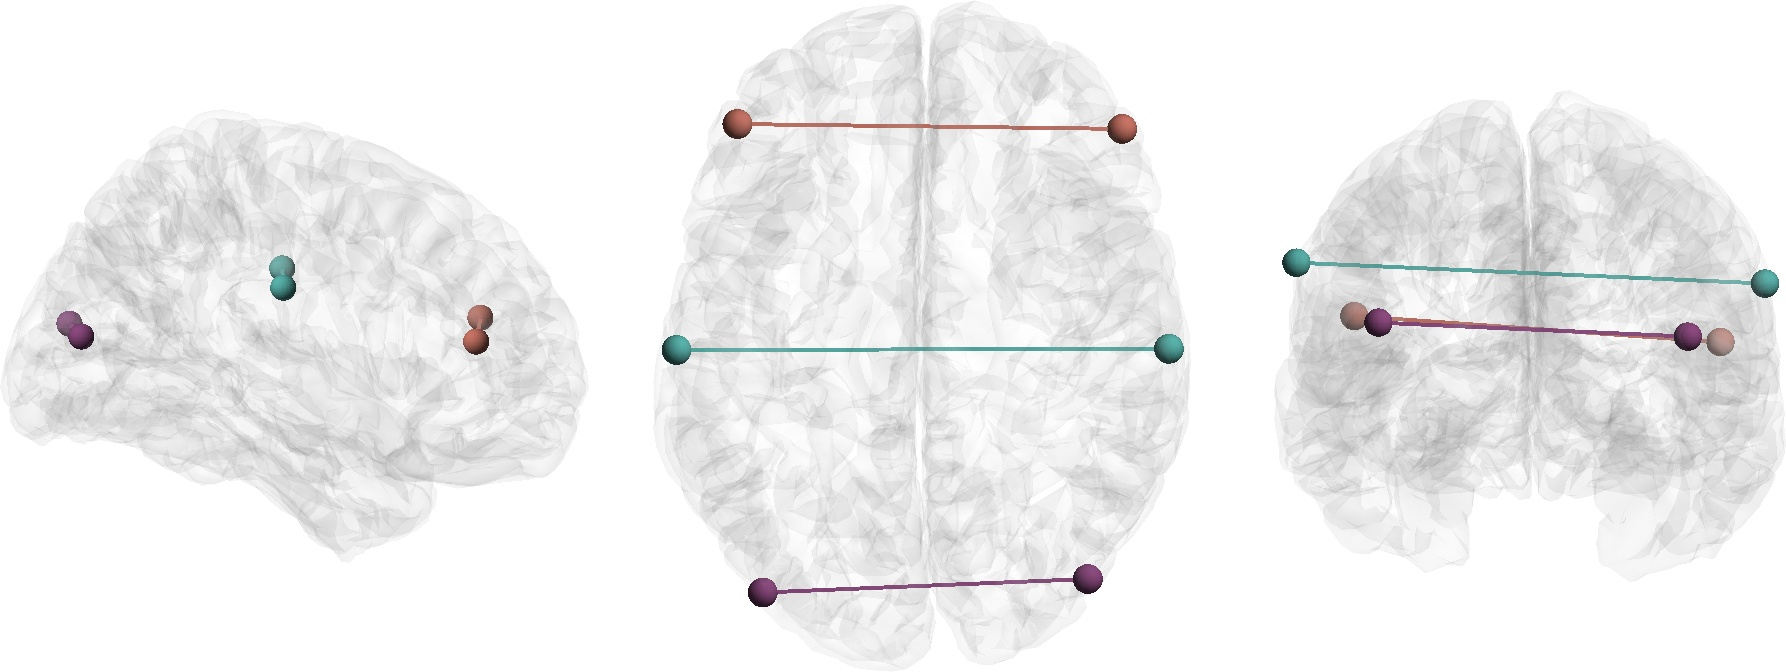
\includegraphics[width=0.99\textwidth]{../images/networks_gopsiicos.jpg}
        \caption{Восстановленные сети, $\phi=\pi/20$}\label{fig:gopsiicos_a}
    \end{subfigure}
    \begin{subfigure}[t]{0.4\textwidth}
        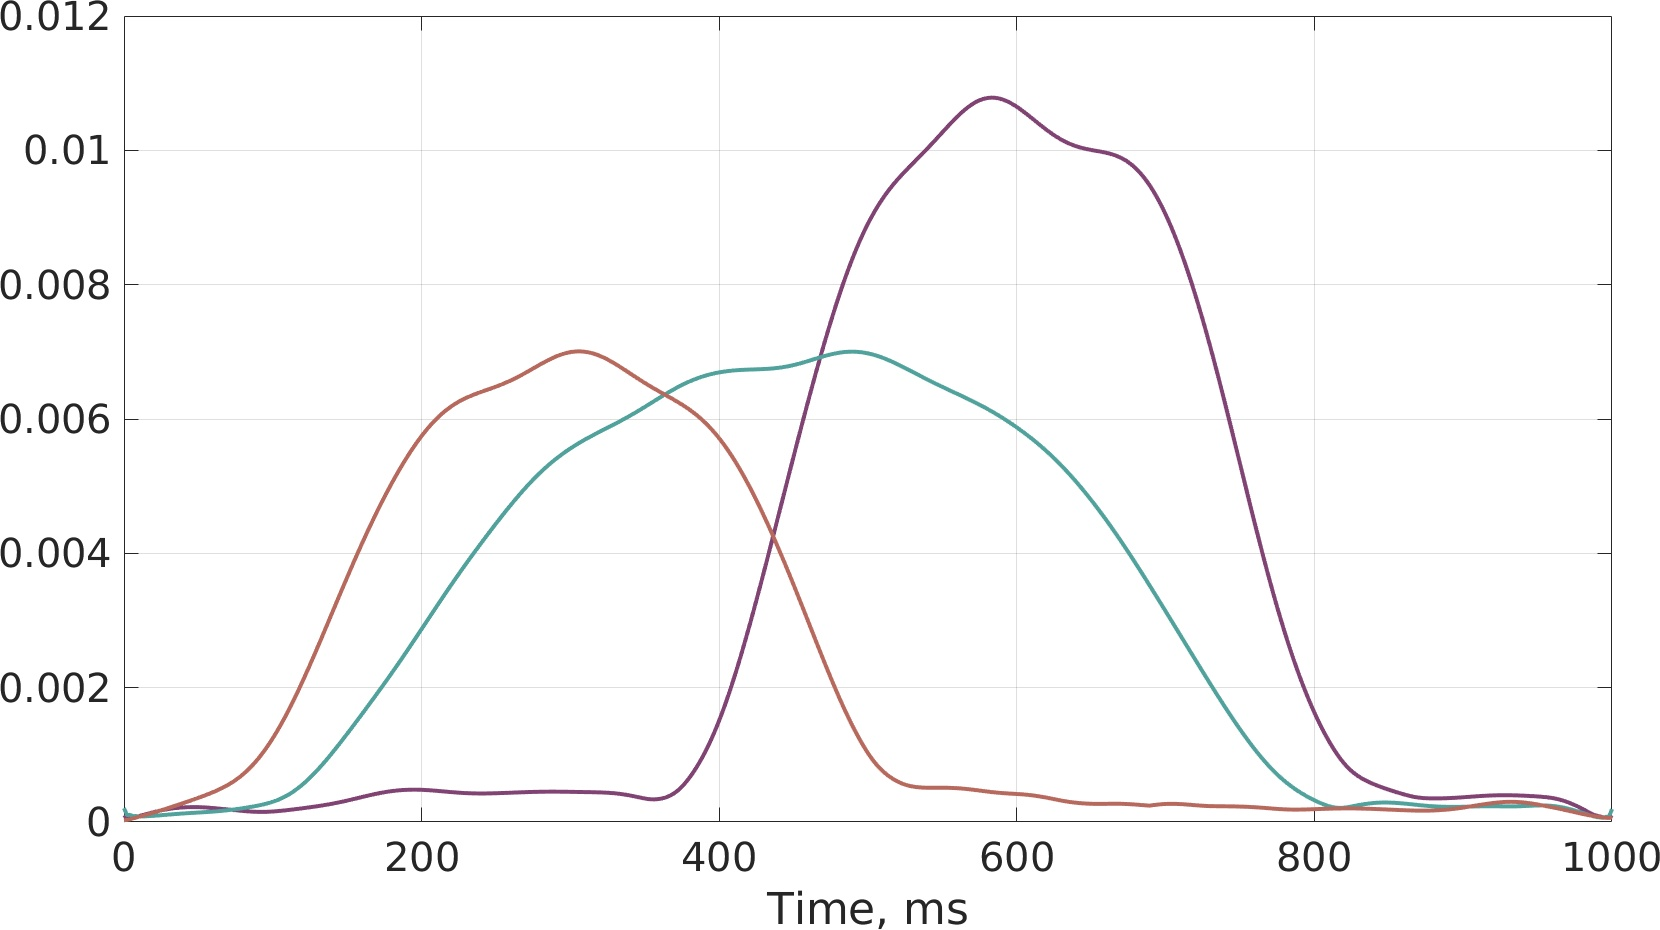
\includegraphics[width=0.99\linewidth]{../images/timeseries_gopsiicos.jpg}
        \caption{Восстановленные профили активации $\phi=\pi/20$}\label{fig:gopsiicos_b}
    \end{subfigure}
    \begin{subfigure}[t]{0.6\textwidth}
        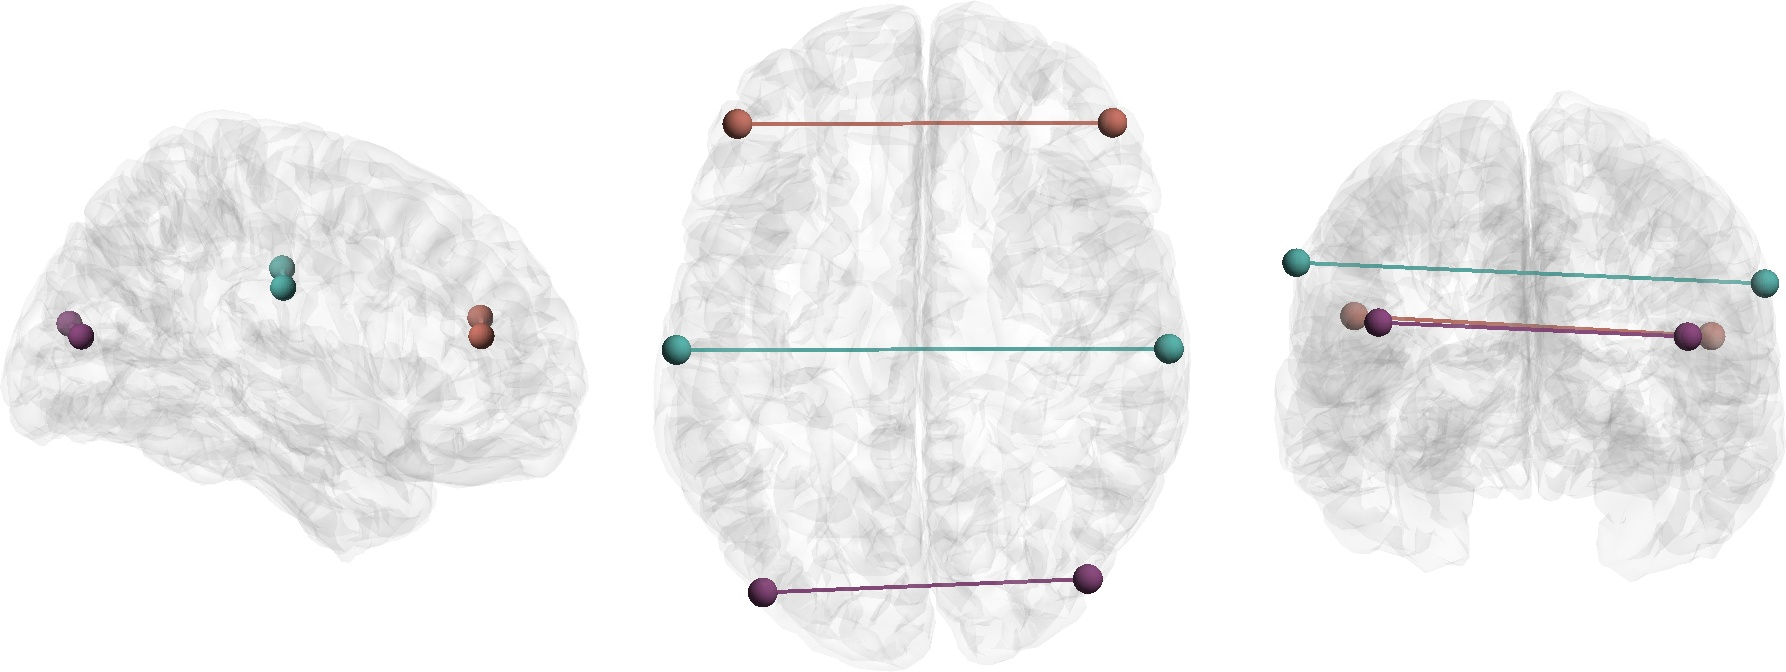
\includegraphics[width=0.99\textwidth]{../images/networks_gopsiicos_pi4.jpg}
        \caption{Восстановленные сети, $\phi=\pi/4$}\label{fig:gopsiicos_c}
    \end{subfigure}
    \begin{subfigure}[t]{0.4\textwidth}
        \includegraphics[width=0.99\linewidth]{../images/timeseries_gopsiicos_pi4.jpg}
        \caption{Восстановленные профили активации $\phi=\pi/4$}\label{fig:gopsiicos_d}
    \end{subfigure}
    \begin{subfigure}[t]{0.6\textwidth}
        \includegraphics[width=0.99\textwidth]{../images/networks_gopsiicos_pi2pi20.jpg}
        \caption{Восстановленные сети, $\phi=\pi/2-\pi/20$}\label{fig:gopsiicos_e}
    \end{subfigure}
    \begin{subfigure}[t]{0.4\textwidth}
        \includegraphics[width=0.99\linewidth]{../images/timeseries_gopsiicos_pi2pi20.jpg}
        \caption{Восстановленные профили активации $\phi=\pi/2-\pi/20$}\label{fig:gopsiicos_f}
    \end{subfigure}
    \caption{Применение метода GO-PSIICOS к задаче детекции трех сетей с перекрывающимися профилями активности для ОСШ=0.5 и фазовых сдвигов $\phi=\pi/20, \phi=\pi/4, \phi=\pi/2-\pi/20$.}\label{fig:gopsiicos}
    Цвета сетей на панели~\ref{fig:gopsiicos_a} соответствуют цветам восстановленных
    профилей на панели~\ref{fig:gopsiicos_b}.
\end{figure}

Для демонстрации работы метода мы использовали симуляции с тремя
сетями с перекрывающимися профилями активности, описанные в разд.~\ref{sec:three_ntw}.
Результаты работы метода для ОСШ=0.5 представлены на рис.~\ref{fig:gopsiicos}.

Как видно на графике, алгоритм справился с нахождением всех трех сетей и достаточно
точно восстановил их временные профили.
           % Глава 3
% \chapter*{Заключение}						% Заголовок
\addcontentsline{toc}{chapter}{Заключение}	% Добавляем его в оглавление

%% Согласно ГОСТ Р 7.0.11-2011:
%% 5.3.3 В заключении диссертации излагают итоги выполненного исследования, рекомендации, перспективы дальнейшей разработки темы.
%% 9.2.3 В заключении автореферата диссертации излагают итоги данного исследования, рекомендации и перспективы дальнейшей разработки темы.
%% Поэтому имеет смысл сделать эту часть общей и загрузить из одного файла в автореферат и в диссертацию:

Основные результаты работы заключаются в следующем.
%% Согласно ГОСТ Р 7.0.11-2011:
%% 5.3.3 В заключении диссертации излагают итоги выполненного исследования, рекомендации, перспективы дальнейшей разработки темы.
%% 9.2.3 В заключении автореферата диссертации излагают итоги данного исследования, рекомендации и перспективы дальнейшей разработки темы.

Мы описали новый метод обнаружения фазовой связности в выделенной полосе
частот, по неинвазивным данным МЭГ/ЭЭГ. Предложенный подход демонстрирует,
возможность выделять истинную линейную связь с нулевым сдвигом по фазе по
неинвазивными записям.  Это достигается за счет предложенной процедуры
проекции, работающей в пространстве сенсоров на кросс-спектральных матрицах и
позволяющей эффективно подавить вклад пространственной протечки сигнала в
действительную часть кросс-спектральной матрицы. Оказывается, что хотя
подпространство, модулируемое действительной частью исходного кросс-спектра и
подпространство, включающее мощность протечки сигнала перекрываются, достаточно
просто построить пространственный проектор, чтобы подавить большую часть
протечки сигнала.  (например, 95, см. рис. 3), и при этом сохранить
чувствительность к большинству источников с нулевой фазовой связью. Как
показано на примере численного моделирования, предлагаемая методика позволяет
сохранить чувствительность для всего диапазона значений фазового сдвига, см. рис. 9.

Используя реалистичное моделирование, мы исследовали предлагаемую методику
(PSIICOS) и сравненили ее эффективность с набором других методов, таких как
DICS, iDICS, а также методом геометрической коррекции (GCS). Метод PSIICOS
стабильно превосходил три референтных метода в обеих смоделированных конфигурациях:
как с тремя сетями с перекрывающимися профилями активности и фиксированными положениями
узлов, так и в случае симуляций Монте-Карло на широком диапазоне реалистичных
условий зашумленности, а также значений фазового сдвига.  Важно отметить, что
метод PSIICOS показал равномерное качество решений для всего диапазона средних
значений фазового сдвига.

В последние годы появилось большое количество методов обнаружения
функциональной связности.  Если бы мы имели доступ к истинным сигналам на коре,
отражающим активность каждого отдельного узла сети, то можно было бы
использовать функцию когерентности, отражающую линейную (с точки зрения теории
линейных стационарных систем) связь между сигналами.  Однако активность
корковых генераторов, измеренная неинвазивно, доступна только в виде смеси
сигналов активации из нескольких источников и, таким образом, прямое
использование сигнала сенсоров приводят к ошибочным результатам: эффект
протечки сигнала маскирует истинную функциональную связь. Для решения этой
проблемы (Nolte et al.(2004a)) предложил использовать мнимую часть
кросс-спектра в качестве статистики на уровне сенсоров, которая не чувствительна к
протечке сигнала.

Это вызвало появление ряда методов, например (Stam et al. (2007), Vinck et al.
(2011), Эвальд и др. (2014)), использующих мнимую часть кросс-спектра на уровне
сенсоров.  Хотя некоторые из них и дают преимущество перед методом imCoh, все
они не в способны обнаруживать сети с нулевой фазовой задержкой, так как мнимая
часть когеренции функционально независима от действительной части исходного
кросс-спектра в пространстве источников, который несет информацию об истинной
связности с нулевой разностью фаз. Для нулевых или близких к нулю средних
фазовых сдвигов ОСШ мнимой части кросс-спектра на уровне сенсоров недостаточно
для надежной детекции, см. рис. 9. В то же время, использование необработанной
действительной части кросс-спектра не представляется возможным из-за эффекта
пространственной протечки. Как мы показали в данной работе, использование
обратного оператора на базе LCMV для разделения данных сенсоров, как это
предлагается в методике DICS, не обеспечивает необходимой точности, а
последующее использование когерентности в пространстве
источников не позволяет получать решения удовлетворительного качества при
реалистичных значениях ОСШ.

Представленный здесь подход наиболее тесно связан со схемой геометрической
коррекции (GCS, Wens et al., 2015), первоначально введенной в применение для
анализа связи между огибающими сигналов в пространстве источников в качестве
альтернативы методам ортогонализации на основе временной структуры активации,
(Hipp et al., 2012), (Colclough et al., 2015). Подход GCS предполагает
использование топографии фиксированного узла в сочетании с фильтром на основе
обратного оператора для некоторого другого источника с которым меряется
связность фиксированного узла. Метод GCS устраняет эффект пространственной
протечки, связанный только с этим фиксированным источником.  В сравнении с этим
вместо использования топографии фиксированного источника и устранения эффекта
протечки сигнала только от него, подход PSIICOS работает в пространстве внешних
произведений топографий пар источников и предполагает создание проектора,
который учитывает вклад в протечку сигнала от всех возможных источников.
Использование сингулярного разложения позволяет построить эффективный оператор
проекции, позволяющий сконцентрировать наибольшее количество нежелательной
мощности протечки сигнала в подпространстве фиксированного ранга. Эта операция
проецирования применяется к матрице кросс-спектра в пространстве сенсоров.

Подобно GCS, PSIICOS позволяет визуализировать динамику отражающего картину
взаимодействий кросс-спектра в пространстве сенсоров и позволяет проводить анализ
в том числе не переходя в пространство источников (применение к анализу на уровне сенсоров
в данной работе не рассматривается). Например,
учитывая растущую значимость методов машинного обучения в анализе
нейрофизиологических данных, операция проекции, составляющая основу PSIICOS,
позволяет получать признаки, отражающие истинную связность в
относительно компактном пространстве сигналов на сенсорах. Проекция PSIICOS также
может быть применена к отдельным векторизованным внешним произведениям
данных на уровне сенсоров, а затем использована для обнаружения корковых участков со
значимыми корреляциями огибающих.

Как мы показали, подход с использованием порождающего уравнения позволяет
интерпретировать задачу оценки параметров порождающей модели кросс-спектра (c
ij) как стандартную недоопределенную проблему линейной регрессии,
распространенную в неинвазивных методах нейровизуализации.  Такой подход
позволяет получить четкий способ введения столь необходимой априорной
информации в задачу оценки связности. Эта информация может быть получена с
помощью диффузионной тензорной визуализации и представлена с использованием
вероятностного распределения, которое затем естественным образом используется в
рамках Байесовской парадигмы.
Менее специфичные, упрощенные априорные распределения, основанные на
пространственной разреженности, также могут быть использованы, и подход,
аналогичный описанному в (Strohmeier et al., 2016), основанный на смешанных
дробных нормах, может быть использован для построения
разреженных решателей, объясняющих наблюдаемый пространственный кросс-спектр на
уровне сенсоров активностью небольшого числа элементарных сетей в пространстве
источников.

Также, следуя по пути параметрического оценивания, можно PSIICOS позволяет применять
обобщения методов подгонки диполя, включая модифицированный алгоритм RAP-MUSIC, примененный к
матрице кросс-спектра с удаленной протечкой сигнала. Фактически, (Ewald et al. (2014)) описывает
использование MUSIC-подхода для анализа мнимой части кросс-спектра на
основе MUSIC-метрик, но, как уже отмечалось ранее, из-за использования только
мнимой части кросс-спектра, предлагаемый подход не чувствителен к сетям с
нулевыми фазовыми задержками. Кроме того, время вычисления для метода, описанного в
(Ewald et al. (2014)), велико, и авторы прибегают к двухэтапной процедуре,
чтобы избежать сканирования по $N^2$ парам источников.
Векторизованная форма кросс-спектра и соответствующее порождающее уравнение могут послужить основой
для разработки подхода RAP-MUSIC, при котором элементарные сети заменяют диполи
в исходных выкладках для этой методики (Мошер и Лихи (1999)). RAP-MUSIC
предполагает построение рекурсивных проекций от подпространства, образуемого
топографиями источников, обнаруженных на предыдущих итерациях. При применении к
векторизованному кросс-спектру для удаления обнаруженной элементарной сети,
состоящей из узлов А и В, такая проекция удалит только вклад конкретной
пары, а спроецированный кросс-спектр сохранит остальные сети, образованные источником А,
со всеми остальными источниками, за исключением узла В, а также сети, образованные источником В,
со всеми остальными источниками кроме А. Это означает, что при применении
подхода RAP-MUSIC к векторизованному кросс-спектру с удаленной протечкой сигнала мы можем
получить возможность исследовать сложные сети, состоящие более чем из одной
пары узлов. Отдельного изучения требует вопрос, решает ли эта процедура проблему, поднятую в работе
Mahjoory et al. (2017), что оценки, полученные методом бимформинга, и глобальные решения MNE
приводят к разным картинам распределения связности.

В текущей векторизованной реализации в среде MATLAB расчет проекционной матрицы
для модели пространства источников с 7000 узлами занимает менее одной секунды
расчетного времени и требует вычисления лишь одинажды для каждого испытуемого,
если предположить, что положения сенсоров фиксированы или что в данных была
сделана поправка на движения испытуемого (такая поправка возможна
использованием метода tSSS).  Векторизованная реализация сканирования по
пространству источников размером 7000 на 7000 узлов занимает полсекунды
вычислительного времени на современном ноутбуке.  Таким образом предложенный
подход является вычислительно эффективным и делает возможным проведение анализа
на основе симуляций Монте-Карло для исследования устойчивости наблюдаемых
сетей, аналогичного проведенному в данной работе.

Современные метрики взаимодействия в пространстве источников для MEG/EEG,
игнорирующие связь с нулевым сдвигом по фазе, приводят как к ложноположительным
Matias Palva и др. (2018), так и к ложноотрицательным срабатываниям. Хотя первая проблема была
решена недавно (например, Wang et al. (2018)), решение второй проблемы до сих
пор не было предложено. В этой работе мы приводим первую демонстрацию
возможности неинвазивного картирования истинной мгновенной линейной связности.
Учитывая убедительные доказательства существования такой малолатентной связи,
как это видно при инвазивных исследованиях на животных, мы полагаем, что
описанная здесь методика PSIICOS значительно расширит возможности современных
функциональных инструментов сетевого анализа.

% Strengths and limitations of PSIICOS framework

Предложенный здесь подход представляет собой новое решение для изучения
взаимодействий в данных МЭГ и может выборочно решать проблему пространственной
протечки даже в случае нулевой или близкой к нулю фазовой связности. Это
позволяет преодолеть ограничения, присущие методам, использующим мнимую часть
кросс-спектра или основанные на временной структуре данных ортогонализационные
подходы, которые по определению игнорируют нулевые фазовые взаимодействия (и
имеют слабую чувствительность к околонулевым фазовым сдвигам). Отметим, однако,
что PSIICOS требует статистической процедуры, основанной на бутстраппинге, и
что он не полностью застрахован от ложноположительных срабатываний при наличии
несвязанных источников с профилями мощности, которые значительно выше, чем у
взаимодействующих источников.

Основное внимание в данной работе мы уделяем новой проекционной схеме,
позволяющей существенно подавить вклад пространственной протечки в кросс-спектр на уровне сенсоров
и получить новое порождающее уравнение (9), позволяющее представить задачу
оценки фазовой связности как задачу оценки источника, но в пространстве пар
сигналов сенсоров. Для проведения необходимой валидации метода мы
выбрали максимально простую стратегию поиска источников для этого уравнения.
Даже при таком простом подходе к оценке наши результаты демонстрируют потенциально
более высокую производительность предлагаемой методики по сравнению с рядом
других релевантных методов и почти одинаковую чувствительность ко всему
диапазону средних значений разности фаз между временными рядами связанных
источников, включая нулевую и близкую к нулю фазовые задержки. Основываясь на
работе, описанной в работе Дарваса F (2005), мы также предложили процедуру
бутстрапа, которая может быть использована для проверки стабильности
наблюдаемого результата.

В случае наличия в данных истинной связности предлагаемая процедура бутстрапа 
имеет низкую вероятность генерации сети из пары активных, но функционально
не связанных источников, до тех пор, пока мощность этих источников
не будет существенно превышать мощность в узлах истинных сетей.
Если данные содержат несколько не связанных между собой функционально, но обладающих высокой мощностью
источников, предлагаемая процедура может привести к ложным срабатываниям. Кроме
того, учитывая описанный способ отбора сетей по верхним значениям метрики
сканирования $\rho$, мы, скорее всего, упустим некоторые истинные сети.

Лучшим способом решения обеих этих проблем является разработка эффективного
статистического теста, работающего на основе распределения для нулевой гипотезы.
Однако чтобы быть полезным, этот тест должен сохранять распределение мощности
в пространстве сенсоров, разрушая при этом нулевую и близкую к нулю
фазовую связность. Тесты, разработанные до сих пор для оценки линейной
синхронизации, в основном адаптированы к мерам, не чувствительным к мгновенной
связности. Более того, применение методов, основанных на рандомизации временных
рядов компонент ICA, не обеспечивает подходящего решения, когда необходимо
обнаружить связность с околонулевой фазовой задержкой. Для решения этих проблем необходим
подход, основанный на фазовой рандомизации источников,
которая бы уничтожала взаимные фазы, но сохраняла бы плавность фазового ответа
отдельных активаций. Однако, поскольку алгоритмы генерации суррогатных данных
соответствуют свойствам исходных данных в пространстве сенсоров (Хауфе и Эвальд 2016 г.),
то пользуясь такими методами может быть трудно отличить мгновенную корреляцию,
вызванную исключительно объемной проводимостью, от истинной связи с нулевой разностью фаз.
Поэтому необходимы более консолидированные усилия для создания надежной системы
статистического тестирования, адаптированной к методам анализа связи, таким как
описанная здесь.

Несмотря на эти ограничения, PSIICOS представляет собой первую попытку
обнаружить по данным МЭГ взаимодействие с нулевой и близкой к нулю фазовой
задержкой.  Насколько нам известно, задача оценки линейного взаимодействия на
основе MEG/EEG впервые представлена как многомерная регрессионная задача,
аналогичная той, которая встречается в классической обратной задаче для этого
типа данных. Такое рассмотрение открывает богатый спектр возможностей для
адаптации множества регуляризационных или параметрических методик,
разработанных в этой области, для решения проблемы оценки функциональной связи.

\begin{enumerate}
  \item Был проведен обзор исследований изменения функциональной коннективности
      мозга при различных паталогиях.
  \item Был разработан метод очистки данных ЭЭГ и МЭГ от протечки сигнала, на
      основе которого было разработано семейство алгоритмов оценки фазовой синхронности,
      позволяющих находить сети с близкими к нулю фазовыми задержками.
  \item Задача оценки фазовой синхронности в условиях протечки сигнала была
      сформулирована и решена как задача оптимальной фильтрации.
  \item Был предложен алгоритм, позволяющий обнаруживать сети с близкими
      к нулю фазовыми задержками, оптимальный в глобальном смысле и позволяющий
      справиться с проблемой ложноположительных срабатываний второго рода, вызванных
      протечкой сигнала.
  \item Было проведено численное исследование свойств предложенной
      проекции, показавшее, что разработанная методика позволяет
      подавить вклад подпространства протечки сигнала в оцененную
      на сенсорах матрицу кросс-спектральной плотности мощности.
  \item Численное исследование свойств метода проекции показало, что
      разработанная методика позволяет находить сети с близкими к нулю фазовыми задержками в условиях
      неинвазивных МЭГ измерений, которые характеризуются значительной протечкой
      сигнала между источниками.
  \item Сравнение с имеющимися на данный момент алгоритмами оценки коннективности
      по неинвазивным данным на основе симуляций показало значительное превосходство
      предложенной техники обнаружения сетей в условиях малых фазовых задержек.
  \item Применение метода очистки от протечки сигнала к реальным данным позволило
      обнаружить физиологически правдоподобные сети, которые невозможно обнаружить
      другими способами.
  \item Было проведенно численное исследование влияния значений ранга предложенной проекции
      на свойства алгоритма, которое позволило получить эвристику для выбора ранга.
  \item Численное исследование влияния неточностей прямой модели на качество решений
      предложенного алгоритма показало, что характерные для реальных записей
      диапазоны ошибок в оценке прямой модели слабо сказываются на качестве
      получаемых решений.
  \item Для выполнения поставленных задач был создан
      пакет утилит в среде MATLAB, в который входят средства генерации тестовых
      данных, визуализации пространственной и временной структуры сетей и наконец
      программные реализации разработанных и использованных для валидации алгоритмов.
  \item Наработки, полученные в ходе работы над данной диссертацией,
      были внедрены в пакеты программ Visbrain и Neuropycon, доступные для публичного
      использования.
\end{enumerate}

% И какая-нибудь заключающая фраза.

% Последний параграф может включать благодарности.  В заключение автор
% выражает благодарность и большую признательность научному руководителю
% Иванову~И.\:И. за поддержку, помощь, обсуждение результатов и научное
% руководство. Также автор благодарит Сидорова~А.\:А. и Петрова~Б.\:Б. за
% помощь в~работе с~образцами, Рабиновича~В.\:В. за предоставленные
% образцы и~обсуждение результатов, Занудятину~Г.\:Г. и авторов шаблона
% *Russian-Phd-LaTeX-Dissertation-Template* за помощь в оформлении
% диссертации. Автор также благодарит много разных людей и
% всех, кто сделал настоящую работу автора возможной.
      % Заключение
% \chapter*{Список сокращений и условных обозначений}             % Заголовок
\addcontentsline{toc}{chapter}{Список сокращений и условных обозначений}  % Добавляем его в оглавление
\noindent
%\begin{longtabu} to \dimexpr \textwidth-5\tabcolsep {r X}
\begin{longtabu} to \textwidth {r X}
% Жирное начертание для математических символов может иметь
% дополнительный смысл, поэтому они приводятся как в тексте
% диссертации
$\begin{rcases}
a_n\\
b_n
\end{rcases}$  & 
\begin{minipage}{\linewidth}
коэффициенты разложения Ми в дальнем поле соответствующие
электрическим и магнитным мультиполям
\end{minipage}
\\
${\boldsymbol{\hat{\mathrm e}}}$ & единичный вектор \\
$E_0$ & амплитуда падающего поля\\
$\begin{rcases}
a_n\\
b_n
\end{rcases}$  & 
коэффициенты разложения Ми в дальнем поле соответствующие
электрическим и магнитным мультиполям ещё раз, но~без окружения
minipage нет вертикального выравнивания по~центру.
\\
$j$ & тип функции Бесселя\\
$k$ & волновой вектор падающей волны\\

$\begin{rcases}
a_n\\
b_n
\end{rcases}$  & 
\begin{minipage}{\linewidth}
\vspace{0.7em}
и снова коэффициенты разложения Ми в дальнем поле соответствующие
электрическим и магнитным мультиполям, теперь окружение minipage есть
и добавлено много текста, так что описание группы условных
обозначений значительно превысило высоту этой группы... Для отбивки
пришлось добавить дополнительные отступы.
\vspace{0.5em}
\end{minipage}
\\
$L$ & общее число слоёв\\
$l$ & номер слоя внутри стратифицированной сферы\\
$\lambda$ & длина волны электромагнитного излучения
в вакууме\\
$n$ & порядок мультиполя\\
$\begin{rcases}
{\mathbf{N}}_{e1n}^{(j)}&{\mathbf{N}}_{o1n}^{(j)}\\
{\mathbf{M}_{o1n}^{(j)}}&{\mathbf{M}_{e1n}^{(j)}}
\end{rcases}$  & сферические векторные гармоники\\
$\mu$  & магнитная проницаемость в вакууме\\
$r,\theta,\phi$ & полярные координаты\\
$\omega$ & частота падающей волны\\

  \textbf{BEM} & boundary element method, метод граничных элементов\\
  \textbf{ЭЭГ} & электроэнцефалография\\
  \textbf{МЭГ} & магнитная электроэнцефалография\\
  \textbf{МРТ} & магнитнo-резонансная томография\\
  \textbf{фМРТ} & функциональная магнитнo-резонансная томография\\
  \textbf{КТ} & компьютерная томография\\
  \textbf{ДТВ} & диффузионно-тензорная визуализация\\
  \textbf{ПЭТ} & позитронно-эмиссионная томография\\
  \textbf{CTC} & communication through coherence; взаимодействие через когерентность\\
  \textbf{PLI} & phase lag index; индекс фазовой задержки\\
  \textbf{wPLI} & weighted phase lag index; взвешенный индекс фазовой задержки\\
  \textbf{ОСШ} & отношение сигнал / шум\\
  \textbf{GCS} & geometric correction scheme

\end{longtabu}
\addtocounter{table}{-1}% Нужно откатить на единицу счетчик номеров таблиц, так как предыдующая таблица сделана для удобства представления информации по ГОСТ
        % Список сокращений и условных обозначений
% \chapter*{Словарь терминов}             % Заголовок
\addcontentsline{toc}{chapter}{Словарь терминов}  % Добавляем его в оглавление

\textbf{TeX} "--- Cистема компьютерной вёрстки, разработанная американским профессором информатики Дональдом Кнутом

\textbf{Панграмма} "--- Короткий текст, использующий все или почти все буквы алфавита
      % Словарь терминов
% \clearpage                                  % В том числе гарантирует, что список литературы в оглавлении будет с правильным номером страницы
%\hypersetup{ urlcolor=black }               % Ссылки делаем чёрными
%\providecommand*{\BibDash}{}                % В стилях ugost2008 отключаем использование тире как разделителя 
\urlstyle{rm}                               % ссылки URL обычным шрифтом
\ifdefmacro{\microtypesetup}{\microtypesetup{protrusion=false}}{} % не рекомендуется применять пакет микротипографики к автоматически генерируемому списку литературы
\insertbibliofull                           % Подключаем Bib-базы
\ifdefmacro{\microtypesetup}{\microtypesetup{protrusion=true}}{}
\urlstyle{tt}                               % возвращаем установки шрифта ссылок URL
%\hypersetup{ urlcolor={urlcolor} }          % Восстанавливаем цвет ссылок
      % Список литературы
% \clearpage
\ifdefmacro{\microtypesetup}{\microtypesetup{protrusion=false}}{} % не рекомендуется применять пакет микротипографики к автоматически генерируемым спискам
\listoffigures  % Список изображений

%%% Список таблиц %%%
% (ГОСТ Р 7.0.11-2011, 5.3.10)
\clearpage
\listoftables   % Список таблиц
\ifdefmacro{\microtypesetup}{\microtypesetup{protrusion=true}}{}
\newpage           % Списки таблиц и изображений (иллюстративный материал)
% \appendix
%%% Оформление заголовков приложений ближе к ГОСТ:
\setlength{\midchapskip}{20pt}
\renewcommand*{\afterchapternum}{\par\nobreak\vskip \midchapskip}
\renewcommand\thechapter{\Asbuk{chapter}} % Чтобы приложения русскими буквами нумеровались
   % Предварительные настройки для правильного подключения Приложений
\chapter{Реализация алгоритма RAP-MUSIC на языке Python}\label{appendix:rap_music_code}

\begin{ListingEnv}[!h]
    \begin{lstlisting}[language=Python,label={rap_music_listing},caption={Алгоритм RAP-MUSIC}]
def RAP_MUSIC(X, G, threshold):
    """
    Параметры
    ---------
    X : матрица измерений
    G : матрица прямой модели для свободной ориентации
    threshold : порог корреляции подпространств

    Возвращает
    ----------
    active_dipole_indices : индексы найденных диполей

    """
    # инициализируем пустой список индексов активных диполей
    active_dipole_indices = []

    while True:
        # ищем корреляции подпространств для каждого источника
        C = MUSIC_scan(X, G)
        if max(C) < threshold:
            break
        k = argmax(C)
        active_dipole_indices.append(k) 
        # проецируем от диполей k-го источника
        X, G = project_away_from_k(X, G, k) 

    return active_dipole_indices
    \end{lstlisting}
\end{ListingEnv}

\chapter{Распределение индуцированной активности по коре в реальных данных}\label{appendix:real_data_power}

Чтобы подтвердить наши выводы и убедиться, что полученные сети не
полностью совпадают с областями коры с доминирующей активностью мы
представили здесь распределение индуцированной активности по коре для целевых частотных диапазонов,
см. рис.~\ref{fig:theta_alpha_pwr},~\ref{fig:beta_pwr},~\ref{fig:gamma_pwr}.
Эти распределения были получены при помощи пакатеа MNE-python в соответствии со следующей процедурой.

Во-первых, чтобы компенсировать разницу в продолжительности эпох из-за
вариабельности времени отклика, мы обрезали каждое испытание в [-0.5, 1.024] секундном
интервале, который соответствовал временному диапазону самой короткой эпохи.
Чтобы смягчить граничные эффекты фильтрации, мы
обратили во времени каждую эпоху и ``приклеили'' ее слев и справа к исходной.
Эти эпохи тройной длины были затем отфильтрованы
в пяти целевых частотных диапазонах КИХ-фильтром с нулевой фазой и переобрезаны
до временного интервала [0,1] секунд, где 0 соответствует моменту предъявления стимула в
исходной неинвертированной эпохе. Далее для пространства источников с 8194
узлами мы вычислили обратный оператор MNE со свободной ориентацией
(коэффициент свободной ориентации = 0,2) и взвешиванием по глубине (коэффициент = 0,6)
и применили его к отдельным испытаниям. Наконец, мы возвели значения для эпох на уровне источников в квадрат и усреднили по времени и по эпохам.
Полученные значения мы нанесли на графики.

\begin{figure}
      \begin{subfigure}[b]{0.5\textwidth}
        \includegraphics[width=\textwidth]{../images/psiicos_paper/Figure16a_hr.jpg}
        \caption{Тета-диапазон}\label{fig:theta_pwr}
      \end{subfigure}
      % \vspace{1cm}
      \begin{subfigure}[b]{0.5\textwidth}
        \includegraphics[width=0.99\textwidth]{../images/psiicos_paper/Figure16b_hr.jpg}
        \caption{Альфа-диапазон}\label{fig:alpha_pwr}
      \end{subfigure}
      \caption{Распределение индуцированной активности в тета (3--6 Гц) и альфа (8--12 Гц) диапазонах}\label{fig:theta_alpha_pwr}
\end{figure} %figure 16

\begin{figure}
    \begin{subfigure}[b]{1\textwidth}
    \includegraphics[width=\textwidth]{../images/psiicos_paper/Figure17_hr.jpg}
    \end{subfigure}
    \caption{Распределение индуцированной активности в бета-диапазоне (16--24 Гц)}\label{fig:beta_pwr}
\end{figure} %figure 17

\begin{figure}
    \begin{subfigure}[b]{0.5\textwidth}
        \includegraphics[width=\textwidth]{../images/psiicos_paper/Figure18a_hr.jpg}
        \caption{Нижний гамма-диапазон}\label{fig:lgama_pwr}
    \end{subfigure}
    % \vspace{1cm}
    \begin{subfigure}[b]{0.5\textwidth}
        \includegraphics[width=0.99\textwidth]{../images/psiicos_paper/Figure18b_hr.jpg}
        \caption{Верхний гамма-диапазон}\label{fig:gama_pwr}
    \end{subfigure}
    \caption{Распределение индуцированной активности в нижнем (30--60 Гц) и верхнем (65--85 Гц) гамма-диапазонах.}\label{fig:gamma_pwr}
\end{figure} %figure 18
        % Приложения

\end{document}
